\documentclass[11pt,a4paper]{article}
\usepackage[T1]{fontenc}
\usepackage[utf8]{inputenc}
\usepackage{lmodern,microtype}
\usepackage{alphalph}
\usepackage[margin=28mm]{geometry}
\usepackage{amsmath,amssymb,amsthm,mathtools}
\usepackage{booktabs,longtable,array,enumitem,fancyvrb}
\usepackage[numbers,sort&compress]{natbib}
\usepackage[hyphens]{url}
\usepackage{xurl}
\usepackage[hidelinks]{hyperref}
\usepackage{bookmark,placeins}
\usepackage{tikz}
\usetikzlibrary{arrows.meta,positioning}
\hypersetup{pdftitle={A fixed-target approach to the sharp iid Berry--Esseen inequality},
 pdfauthor={Bartosz Kołodziejek and Kacper Rodziewicz}}
\setlength{\emergencystretch}{2em}
\setcounter{tocdepth}{1}
\makeatletter
\renewcommand\paragraph{\@startsection{paragraph}{4}{\z@}%
  {2.5ex \@plus1ex \@minus.2ex}{0.8ex \@plus.2ex}%
  {\normalfont\normalsize\bfseries}}
\makeatother
\newcolumntype{P}[1]{>{\raggedright\arraybackslash}p{#1}}
\newtheorem{theorem}{Theorem}[section]
\newtheorem{lemma}[theorem]{Lemma}
\newtheorem{proposition}[theorem]{Proposition}
\newtheorem{corollary}[theorem]{Corollary}
\theoremstyle{definition}
\newtheorem{definition}[theorem]{Definition}
\newtheorem{assumption}[theorem]{Assumption}
\newtheorem{condition}[theorem]{Certificate condition}
\theoremstyle{remark}
\newtheorem{remark}[theorem]{Remark}
\newcommand{\E}{\mathbb E}
\newcommand{\Pp}{\mathbb P}
\newcommand{\R}{\mathbb R}
\newcommand{\N}{\mathbb N}
\newcommand{\CE}{C_{\mathrm E}}
\newcommand{\supp}{\operatorname{supp}}
\newcommand{\Var}{\operatorname{Var}}
\newcommand{\pos}[1]{(#1)_+}
\newcommand{\ind}{\mathbf 1}
\newcommand{\iid}{\mathrm{iid}}
\title{A fixed-target approach to the sharp iid\\
Berry--Esseen inequality\thanks{This paper was written with substantial
assistance from AI systems; see the end of Section~\ref{ms:discussion}.}}
\author{Bartosz Ko{\l}odziejek \and Kacper Rodziewicz}
\date{4 November 2026}
\begin{document}
\maketitle
\begin{abstract}
We prove the sharp iid Berry--Esseen inequality with constant
$\CE=(3+\sqrt{10})/(6\sqrt{2\pi})$ for every sample size.
The proof is computer-assisted: finite exact certificates establish
the numerical inequalities on complete parameter regions. The
normalized optimal constant is strictly below $\CE$ for $n\ge700$;
Esseen's skew-Bernoulli limit makes $\CE$ the sharp global constant.

The central idea is to measure distance from the extremal two-point
law by a nonnegative support-gap defect. Attainment and the contact
condition give a conservation identity relating this defect to an
explicit remainder. Successive bounds confine a possible extremizer,
and conditioning on the signs of its summands reduces the comparison
to binomial counts with centered conditional noise. Polynomial
majorants, a physical comparison at four summands and finite count
comparisons establish a sharp base through $42$.
A one-step smoothing estimate places a first strict failure
in the domain of either a finite or a uniform local comparison, both
of which exclude it. The proof keeps the same marginal throughout
these reductions, includes threshold atoms and closed parameter
boundaries, and separates the analytic reductions from certificate
construction and exact verification.
\end{abstract}
\begingroup\small
\makeatletter
\renewcommand{\l@section}{\@dottedtocline{1}{0em}{1.5em}}
\makeatother
\tableofcontents
\endgroup
\clearpage
\section{The problem, results, and proof strategy}\label{ms:introduction}
\subsection{The problem and the candidate constant}
Let $\mathcal P$ be the laws on $\R$ with mean zero, variance one and
finite third absolute moment $\rho(P)=\E|X|^3$. For independent copies
$X_1,\ldots,X_n$ of $P$, put $S_n=\sum_iX_i$ and
\[
 \Delta_n(P)=\sup_{H\in\R}|\Pp_P(S_n\le H)-\Phi(H/\sqrt n)|,
 \qquad C_n=\sup_{P\in\mathcal P}\frac{\sqrt n\,\Delta_n(P)}{\rho(P)}.
\]
Here $\Phi$ and $\phi$ are the standard normal distribution function
and density. The sharp-constant conjecture is
\begin{equation}\label{ms:conjecture}
 \sup_{n\ge1}C_n=\CE,
 \qquad \CE=\frac{3+\sqrt{10}}{6\sqrt{2\pi}}=0.409732\ldots.
\end{equation}
Throughout, $H$ is a threshold for the unnormalized sum $S_n$, and
a terminating decimal in an inequality denotes the corresponding exact
rational number. Affine standardization gives the equivalent result
for any mean and positive variance, with third absolute central moment
divided by the cube of the standard deviation.

Berry and Esseen established the classical order $n^{-1/2}$
\cite{Berry1941,Esseen1942,Esseen1945}. Esseen's lower bound
\cite{Esseen1956} explains the proposed constant. If
$p_*=(4-\sqrt{10})/2$, $q_*=1-p_*$ and
$X=(B-p_*)/\sqrt{p_*q_*}$ for $B\sim\operatorname{Bernoulli}(p_*)$,
the fixed-law lattice limit gives
\begin{equation}\label{ms:bernoulli-limit}
 \lim_{n\to\infty}\frac{\sqrt n\Delta_n(P)}{\rho(P)}
 =\frac{3+q_*-p_*}{6\sqrt{2\pi}(p_*^2+q_*^2)}=\CE.
\end{equation}
Indeed $p_*^2+q_*^2=10-3\sqrt{10}$ and
$(3+q_*-p_*)/(p_*^2+q_*^2)=3+\sqrt{10}$.
Every constant below $\CE$ therefore fails for a sufficiently large sum
of this one law. The upper conjecture is associated with Zolotarev
\cite{Zolotarev1966,Zolotarev1967}; Schulz proves the strict finite-index
bound for every nondegenerate Bernoulli law \cite{Schulz2016}.


\subsection{Results and their hypotheses}\label{ms:scope}
Theorem~\ref{short:global} proves $C_n\le\CE$ for every $n\ge1$,
with strict inequality for $n\ge700$. The Bernoulli limit above proves
that the global constant cannot be lowered. The proof uses three parts.
\begin{center}\small
\begin{tabular}{@{}P{.25\linewidth}P{.68\linewidth}@{}}
\toprule
Part & Conclusion and role \\
\midrule
Finite induction through $42$ &
The first four indices use polynomial majorants and a physical comparison.
For $5\le n\le42$, actual-index support and Fourier bounds acquire the
hypotheses of finite count comparisons. Each step uses sharp earlier
indices and retains one common marginal throughout. \\
First-failure comparison, Theorem~\ref{ext:bridge-composition} &
At a least index with $C_n>\CE$, a one-step smoothing estimate gives
$n(C_n-\CE)<0.3$, sharp deleted predecessors and zero predecessor loss.
A finite comparison excludes $43\le n\le48$; a uniform comparison
excludes every $n\ge49$. This proves the weak bound for all $n$. \\
Compact strict comparison, Theorem~\ref{short:acquired-exclusion} &
For $n\ge700$, a fixed-target maximizer with nonnegative excess would
have $nD\le32.20665378$ and $|H|\le1.83605680$. These bounds place
it in an explicit conditional-support region where the binomial
comparison is strict, including the zero-noise case. \\
\bottomrule
\end{tabular}
\end{center}
The small-index and localization calculations are computer-assisted.
Their proofs combine continuous analytic bounds, exact inequalities on
closed parameter regions, and checks that successive bounds concern
the same law. Appendix~\ref{revision:reproducibility} identifies the
inputs, complete executions and acceptance procedures. The published
structural and finite-binomial results used in the compact comparison
are stated at \eqref{v9:entry:structural} and
\eqref{short:count:binomial}, with their hypotheses and references.

There is no assumption of a sharp bound through $699$. The finite
induction stops at $42$; the first-failure argument supplies all later
indices at once. The separate compact comparison proves strictness
from $700$ onward. Nor is eventual two-point optimality asserted:
the proof bounds every possible extremal witness without replacing
an unrestricted law by a two-point law.

\subsection{Why the defect controls a maximizer}
At a fixed $n$, maximize the difference between the two sides of the
candidate inequality:
\begin{equation}\label{v9:intro:excess}
 a(P,H)=\sqrt n\{\Pp_P(S_n\le H)-\Phi(H/\sqrt n)\}-\CE\rho(P).
\end{equation}
Proposition~\ref{v9:core:attainment} proves attainment. Its first-order
condition bounds $y\mapsto\Pp(S_{n-1}\le H-y)$ by an explicit
piecewise cubic function that agrees with it on the closed support.
This contact condition allows us to use the geometry of that support.

Let $\tau(t)=\E[X\ind_{\{X\ge t\}}]$ be the zero-bias density and
$J=\sum_g\tau_g|g|^2$, where $g$ runs over bounded support gaps and
$\tau_g$ is the constant value of $\tau$ there. A lattice law of span
$h$ has $J\ge h$; if every successive gap has length $h$, then $J=h$.
Thus $J$ measures gap size with zero-bias weights. The inequality
\[
 \gamma+3J\le(3+\sqrt{10})\rho,\qquad \gamma=\E X^3,
\]
proved in Lemma~\ref{ms:physical-defect}, extends the moment--span
bound from lattice laws to arbitrary standardized laws. Its slack
\[
 D=(3+\sqrt{10})\rho-\gamma-3J
\]
is nonnegative and vanishes exactly at the positive-skew Bernoulli
law in \eqref{ms:bernoulli-limit}. The lattice consequence and its
reflection are proved in Corollary~\ref{opus:lattice-gap}.

Integrating the contact relation against $\tau$ in two ways gives the
conservation identity of Theorem~\ref{revision:contact-conservation}.
Since $\CE=(3+\sqrt{10})\phi(0)/6$, its two leading moment terms
combine into a multiple of $D$. Solving for the excess gives
\[
 a=\frac{\mathcal R_c-n\CE\rho(1-e)
             -n\phi(0)eD/6-n^{3/2}L}{n+H^2},
 \qquad e=\exp(-H^2/(2n)).
\]
Here $L\ge0$ is a weighted contribution from the law of $H-S_{n-1}$
inside the support gaps, and $\mathcal R_c$ is an explicitly defined
remainder. The three subtracted terms are nonnegative. A nonnegative
excess therefore requires $n\phi(0)eD/6\le\mathcal R_c$.
Once localization bounds both $\mathcal R_c$ and $|H|$, this bounds
$nD$. The uniform bounds come from Theorem~\ref{v9:entry:theorem},
not from a fixed-law asymptotic expansion.

The predecessor hypothesis supplies an upper bound for
$\Pp(S_{n-1}\le H-t)$ in the contact condition, which excludes remote
support points; see \eqref{v9:entry:contact}. This support argument is
used both in coarse localization and in the final two-ray estimate.
With $nD\le32.20665378$, the geometry at $n\ge700$ gives
$3/8<p<93/200$, inward support displacement below $1/250$ and
$\lambda<7/20$. Count conditioning then compares the law with a
binomial sum. One threshold count controls noise up to $1/100$;
five neighboring counts control the remaining interval. Both
comparisons keep all probabilities entering from other counts.

\begin{figure}[ht]
\centering
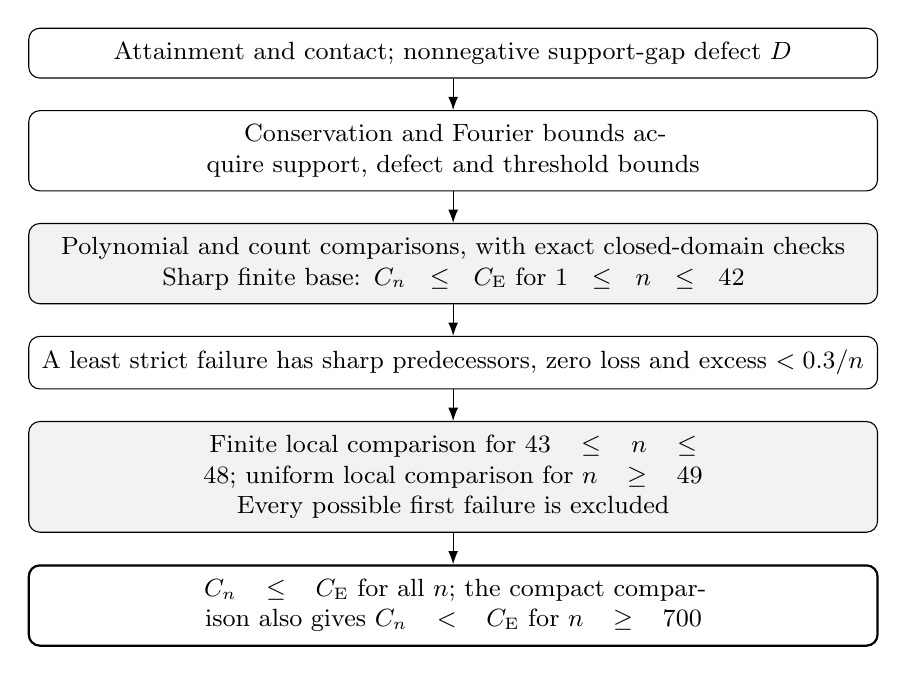
\begin{tikzpicture}[node distance=4mm,>=Latex,
 box/.style={draw,rounded corners,align=center,text width=.86\linewidth,
 inner sep=5pt,font=\small}]
\node[box] (contact) {Attainment and contact; nonnegative support-gap defect $D$};
\node[box,below=of contact] (identity) {Conservation and Fourier bounds acquire support, defect and threshold bounds};
\node[box,fill=gray!10,below=of identity] (finite) {Polynomial and count comparisons, with exact closed-domain checks\\
Sharp finite base: $C_n\le\CE$ for $1\le n\le42$};
\node[box,below=of finite] (failure) {A least strict failure has sharp predecessors, zero loss and excess $<0.3/n$};
\node[box,fill=gray!10,below=of failure] (local) {Finite local comparison for $43\le n\le48$; uniform local comparison for $n\ge49$\\
Every possible first failure is excluded};
\node[box,line width=.8pt,below=of local] (global) {$C_n\le\CE$ for all $n$; the compact comparison also gives $C_n<\CE$ for $n\ge700$};
\draw[->] (contact)--(identity);
\draw[->] (identity)--(finite);
\draw[->] (finite)--(failure);
\draw[->] (failure)--(local);
\draw[->] (local)--(global);
\end{tikzpicture}
\caption{The proof's main dependencies. The shaded comparisons combine
analytic inequalities with complete exact finite checks. The uniform
comparison is proved for every index in its range; it is not an
extrapolation from the finite calculation.}
\end{figure}

\FloatBarrier
\subsection{What the certificates prove}
A certificate is finite exact data for a specified mathematical inequality,
together with rules for checking those data. Here the claim is always about
an entire region of possible laws or parameters. It is not a claim about
only the distributions or points tried during a numerical search.

The proof uses three forms of certificate. For the first few indices,
rational polynomial coefficients majorize the closed sum event on a whole
support product; independence expresses the expectation through moments of
one common marginal. For localization and Fourier bounds, rational boxes
cover the complete admissible parameter region. A box is either excluded
by a necessary inequality or assigned bounds valid everywhere on it.
For the count comparisons, a finite tree subdivides the acquired probability,
phase and noise region until each terminal cell has a strict score bound
or a proved contradiction. The checker verifies the initial domains,
every subdivision and all terminal inequalities, including shared
boundaries. Thus every possible witness is accounted for.

Finding these data and verifying them are separate tasks. A search can
choose polynomial coefficients, subdivisions, prices or refinement passes.
It may use floating-point calculations to suggest those choices. Acceptance
uses the resulting exact rational data and checks every claimed inequality;
a successful search or a saved success message has no independent authority.
Some of the present candidates are supplied objects whose complete
acceptance is repeated. Other tables are constructed and then recomputed.
The reproduction record distinguishes these cases. Where the constructor
and acceptor share numerical routines, this is described as exact replay,
not as an independent implementation of the same calculation.

Acceptance uses integer and rational arithmetic. Roots, exponentials,
trigonometric functions and Gaussian probabilities are enclosed by rational
bounds with explicit analytic remainders. The main checking programs use
Python integers; the three-summand Bernstein checker uses C++ with
Boost's arbitrary-precision integers. No floating-point approximation is
accepted as an exact sign test. The trusted implementation includes the
checking programs, their arithmetic libraries and their execution environment;
this is a computer-assisted proof, not a proof-assistant formalization.

A passed certificate still needs its mathematical hypotheses. For example,
a count certificate can establish a bound for every law in a prescribed
support and moment region, while a separate localization argument proves
that the same hypothetical maximizing law lies in that region. The
resource-to-count checks verify this implication without changing the
index, the marginal, or the discrepancy orientation. Continuous arguments
such as attainment, contact, Fourier inversion and the least-failure
induction are proved in the text; they do not follow from an arithmetic
success flag.

The appendices give the inequalities implemented by the checkers and the
rules for their domain coverage. Appendix~\ref{revision:reproducibility}
maps the full argument to its numerical families and explains the source
package, commands and execution records. An independent verification needs these derivations,
the exact inputs, the complete acceptors and the checks matching each
output to the next theorem's hypotheses. Hashes identify the files used;
they do not prove the inequalities.

Subdivision and rigorous enclosure have established precedents in
computer-assisted proofs \cite{SolovyevHales2013}. Numerical optimization
also appears in Berry--Esseen estimates \cite[Section~2]{Shevtsova2011}.
The custom JSON files organize this proof's exact data; their format is
not a standard theorem-proving language. The mathematical justification
comes from the inequalities, complete coverage and correct implementation
of the checking rules.

\subsection{Related work}
Fourier and structural moment inequalities progressively improved the
universal upper bound \cite{vanBeek1972,Prawitz1972,Tyurin2010,
Shevtsova2011,Shevtsova2013}. We use Shevtsova's structural inequality
explicitly in localization. Recent manuscripts report smaller upper
constants \cite{xiao2026berryesseen,lin2026berryesseen}, and He and Cheng
report eventual sharpness beyond a uniform, very large threshold
\cite{hecheng2026eventually}. Work on independent arrays and extremizers
addresses the related non-iid problem \cite{BellIndependent2026,
BellExtremizers2026}. These recent reported results are not used in
our proof. An earlier AI-assisted working draft is on Hexagon
\cite{rodziewiczkolodziejek2026momentdefects}.

\subsection{Organization and notation}\label{ms:guide}\label{ms:notation}
Section~\ref{v9:core:section} gives attainment, contact and reflection.
The next two sections develop the defect and the conservation identity.
These are the shared analytic tools. The remaining argument has two routes.
The compact route in Sections~\ref{v9:entry:section}--\ref{short:count:section}
gives strict exclusion at $n\ge700$ from a sharp predecessor.
The extension supplies a finite induction and a different local comparison
that applies at a first strict failure below that threshold as well.

For the logic of the extension, read the one-step estimate in
Section~\ref{ext:smoothing} and the first-failure argument in
Section~\ref{ext:bridge} before the numerical tables. Their conclusion
requires a sharp base through $42$ and two local exclusions.
Section~\ref{ext:starting-cases} treats the first four indices;
Sections~\ref{ext:finite-counts}--\ref{ext:floor40} describe the finite
induction through $42$. Section~\ref{ext:local-engine} explains the two
local exclusions. The continuous estimates and full numerical interfaces
are in the appendices. The assembly criteria state the numerical premises
explicitly, so each can be matched to its reproduction record.

Two optimization problems are used. The finite induction maximizes the
ratio, with attained score $C=C_n$. The compact tail argument maximizes
the excess above the fixed coefficient $c=\CE$. Both give contact,
but their excesses and normalization differ; Corollary~\ref{ext:ratio-attainment}
records the precise relation. Neither route changes the marginal law
while acquiring its successive bounds.

The following table distinguishes the three scales used in the proof.
Gap-specific parameters are introduced after the existence of a central
gap has been established.
\begin{center}\small
\begin{tabular}{@{}P{.27\linewidth}P{.66\linewidth}@{}}
\toprule
Symbol & Meaning and scale \\
\midrule
$H$, $H/\sqrt n$ & Threshold for the original sum; its normal-standardized value. \\
$B_0=\ind_{\{X>0\}}$, $p,q$ & Sign class and its probabilities for the original marginal. \\
$m$, $\ell=m/(pq)$ & $m=\E X_+=\E X_-$; distance between conditional means. \\
$W$, $\theta=\E W^2$ & $W=X-\E(X\mid B_0)$; conditional noise in original units. \\
$U=W/\ell$, $s=\E U^2$, $\lambda=ns$ & Noise in count units; marginal and total noise variances. \\
$t=np+H\sqrt{pq+s}=k+u$ & Count threshold, integer anchor, and phase. \\
$a_0,a_1$, $d=a_0+a_1$ & Inward support displacements in count units. \\
$J$, $D$ & Weighted support-gap sum and defect of the original law. \\
\bottomrule
\end{tabular}
\end{center}
The exact normalization is proved in \eqref{ms:bernoulli-coordinates}.
It identifies the count-coordinate law with the original $X$ and leaves
$H$ as its raw sum threshold. The signed moments are
$\gamma=\E X^3$ and $\beta=\E[X|X|]$.

\section{Fixed-target extremizers and contact}
\label{v9:core:section}

We maximize the difference between the two sides of the desired
inequality. Its sign detects failure of the target bound, while the
coefficient of the third absolute moment is fixed in advance.
Throughout, sums have
independent identically distributed summands with mean zero, variance one
and finite third absolute moment $\rho$. Fix $n\ge2$, $c>0$, and a real
raw sum threshold $H$. Set
\begin{gather*}
 z=H/\sqrt n,\quad F=\Pp(S_n\le H),\quad
 a=\sqrt n\{F-\Phi(z)\}-c\rho,\\
 \phi_z=\phi(z),\quad\beta=\E[X|X|],\quad\gamma=\E X^3.
\end{gather*}
In particular $a$ is not divided by $\rho$.

\subsection{Attainment, contamination and the entire closed support}

\begin{proposition}\label{v9:core:attainment}
For each fixed $n$ and $c>0$, the supremum of $a$ over these laws and
thresholds is attained, and the closed-CDF discrepancy at every attaining
pair is positive.
At every maximizing pair,
\begin{align}
 I(y)={}&n^{3/2}\{h(y)-F\}+ny\phi_z
       +\tfrac12H\phi_z(y^2-1)\notag\\
 &+\tfrac32c\rho(y^2-1)-c\{|y|^3-\rho-3y\beta\}\le0,
 \qquad h(y)=\Pp(S_{n-1}\le H-y),\label{v9:core:contact}
\end{align}
with equality on the whole closed support. That support is compact.
Neither statement assumes $a\ge0$ or $H\ge0$.
\end{proposition}
Equivalently, $\Delta=Q-h\ge0$ everywhere and $\Delta=0$ on the closed
support, where
\begin{equation}\label{v9:core:Q}
 Q(y)=F+\frac{H\phi_z+c\rho}{2n^{3/2}}
 -\frac{n\phi_z+3c\beta}{n^{3/2}}y
 -\frac{H\phi_z+3c\rho}{2n^{3/2}}y^2
 +\frac c{n^{3/2}}|y|^3.
\end{equation}

The contact condition is a first-order optimality condition: replacing one
summand by a fixed value $y$ gives the conditional probability $h(y)$.
After recentering and rescaling the perturbed law, the directional
change of the excess is nonpositive. Its average against $P$ is zero,
which forces equality on the closed support. The function $Q$ is
piecewise cubic because it contains $|y|^3$.

\begin{proof}
Write $a^*$ for the supremum. Since $\rho\ge1$ and the discrepancy is
at most one, $a^*\le\sqrt n-c$. Symmetric Bernoulli evaluated at $H=n$
gives $a^*\ge\sqrt n(1-\Phi(\sqrt n))-c>-c$.
For a maximizing sequence, $a_j\to a^*$ and
$c\rho_j\le\sqrt n-a_j$ give a common third-moment ceiling.
The discrepancies satisfy $\sqrt n(F_j-\Phi(H_j/\sqrt n))
=a_j+c\rho_j\ge a_j+c>\eta$ eventually for some $\eta>0$.
Chebyshev bounds the negative threshold tail by $n/H_j^2$;
the positive discrepancy is at most the normal tail, also at most
$n/H_j^2$. Thus $H_j$ is bounded.

Tightness gives a subsequence $P_j\Rightarrow P$, $H_j\to H$ and
$\rho_j\to b$. The common third-moment ceiling $M$ gives tail
bounds $\int_{|x|>K}x^2dP_j\le M/K$ and
$\int_{|x|>K}|x|dP_j\le M/K^2$. Bounded continuous truncations
therefore preserve mean and variance. Lower semicontinuity gives
$1\le\rho(P)\le b$. For fixed $n$, the sum laws converge weakly.
Applying the closed-set inequality first at $H+t$ and then letting
$t\downarrow0$ gives
$\limsup F_j(H_j)\le F_P(H)$, including an atom at $H$.
Consequently
\[
 a(P,H)\ge a^*+c\{b-\rho(P)\}\ge a^*.
\]
Maximality forces equality and $\rho(P)=b$. Thus third moments converge along this maximizing sequence. The discrepancy remains positive since $a^*+c\rho\ge a^*+c>0$.

The contact inequality is a first-variation condition. To obtain it,
contaminate the raw marginal by
$(1-\epsilon)P+\epsilon\delta_y$. Its mean is $\epsilon y$,
variance $v_\epsilon=1+\epsilon(y^2-1)-\epsilon^2y^2$, and centered
third absolute moment has derivative $|y|^3-\rho-3y\beta$ at zero.
The last assertion follows by dominated differentiation of
$|x-\epsilon y|^3$, with bound $3|y|(|x|+|y|)^2$.
Evaluate the standardized law at the standardized image of the fixed
raw event $S_n\le H$. The raw event probability is a polynomial in
$\epsilon$, with derivative $n(h(y)-F)$ even at an atom collision.
The normal argument is
$(H-n\epsilon y)/\sqrt{nv_\epsilon}$, whose derivative is
$-\sqrt n y-H(y^2-1)/(2\sqrt n)$.
The one-sided derivative of the excess is exactly \eqref{v9:core:contact};
maximality makes it nonpositive.

Its integral against $P$ is zero. All terms are integrable.
The closed-event map $h$ is upper semicontinuous; at an atom it takes
the larger one-sided value. Thus $I$ is upper semicontinuous. Strict
negativity at a closed-support point would hold with a uniform negative
margin on a neighborhood of positive $P$-mass, contradicting its zero
integral. Finally $I(y)\le-c|y|^3+C_2y^2+C_1|y|+C_0$ for constants
depending on this pair. It is strictly negative on both sufficiently
distant rays, proving compact support.
\end{proof}

\subsection{Reflection, equality, and the first unresolved index}
\label{v9:core:reflection}
The sign of the attained maximum detects failure of the strict bound $C_n<c$,
including equality. If $C_n$ denotes the supremum of the normalized
absolute discrepancy, reflection gives, including an atom at $H$,
\[
 \Pp(-S_n\le-H)-\Phi(-z)
 =\Phi(z)-\Pp(S_n<H)\ge\Phi(z)-F.
\]
Thus each negative closed-CDF error is bounded by a positive closed-CDF
error of the reflected law; equality at an atom is not assumed.
Consequently $C_n$ is also the supremum of positive
closed scores $r$. Since $a=\rho(r-c)$, $C_n<c$ gives
$a^*\le C_n-c<0$, and $C_n>c$ gives $a^*>0$. If $C_n=c$, choose
$r_j\uparrow c$ with $r_j\ge c/2$. Then
$\rho_j\le2\sqrt n/c$, so $\rho_j(r_j-c)\to0$ and $a^*=0$.
Hence $C_n\ge c$ supplies an attained pair with $a\ge0$.

\begin{corollary}[Ratio extremizers from fixed-target attainment]
\label{ext:ratio-attainment}
For every $n\ge2$, the constant $C_n$ is attained as a positive
closed-CDF score by a compactly supported standardized law and a raw
threshold $H$. This pair maximizes the fixed-target excess at $c=C_n$,
with maximum zero. In particular, it satisfies
\eqref{v9:core:contact} with $c=C_n$.
\end{corollary}
\begin{proof}
The inequality $\rho\ge1$ gives $C_n\le\sqrt n$. Symmetric Bernoulli
at $H=n$ gives $C_n\ge\sqrt n\{1-\Phi(\sqrt n)\}>0$.
Set $c=C_n$ in the preceding argument. Every excess is nonpositive,
and scores $r_j\uparrow C_n$ with $r_j\ge C_n/2$ satisfy
$\rho_j\le2\sqrt n/C_n$, so their excesses tend to zero.
Proposition~\ref{v9:core:attainment} attains this zero maximum.
At an attaining pair, $\rho(r-C_n)=0$ and $\rho>0$, hence $r=C_n$.
The same proposition gives compact support and contact.
\end{proof}

This corollary provides the extremizers used by the finite-index
arguments. Their target coefficient is the unknown extremal ratio
$C_n$, whereas the large-index argument fixes the coefficient at $\CE$.
The contact expressions agree after the normalization
$I_{\mathrm{fixed}}=\rho I_{\mathrm{ratio}}$ at $c=C_n$.
An extremizer of the ratio need not maximize the excess at $\CE$:
its excess there is $\rho(C_n-\CE)$. Each estimate below specifies
which of these two optimization problems it uses.

\begin{corollary}[First failure of a strict bound]\label{v9:core:first-failure}
Assume a genuine finite base $C_j\le c$ for $1\le j<N$. If a strict
bound $C_n<c$ fails at any index $n\ge N$, there is a least such index,
an attained fixed-target pair with $a\ge0$, and predecessor bounds
$C_j\le c$ for every $j<n$. The bounds are strict for $N\le j<n$.
\end{corollary}
\begin{proof}
The nonempty set of failing indices at least $N$ has a least member.
The preceding equivalence supplies its maximizing pair. Indices below
$N$ use the finite base; the other earlier indices use minimality.
\end{proof}
Thus an argument excluding every such pair for $n\ge N$ would give
strict bounds above the finite base, including exclusion of equality.
The subsequent entry argument uses only $C_{n-1}\le c$; it does not
use an upper bound for the actual score $c+a/\rho$. The finite base
and the eventual exclusion remain separate obligations.

\subsection{Two elementary moment domains}\label{ms:moment-domain}

These two inequalities restrict the signed moments in terms of $\rho$.
They hold for every standardized law with finite third moment, including
laws of unbounded support.

\begin{theorem}[Signed and absolute third moments]\label{ms:sharp-third}
If $\E X=0$, $\E X^2=1$, $\rho=\E|X|^3<\infty$, and
$\gamma=\E X^3$, then
\[
 \rho\ge\frac{\gamma^2+2}{\sqrt{\gamma^2+4}}.
\]
\end{theorem}
This is the sharp moment relation of Shevtsova
\cite{shevtsova2014complex}; in the cited arXiv version its equivalent
form is Theorem~2. The following factorization gives a self-contained proof.
\begin{proof}
Set $s=\sqrt{\gamma^2+4}$, $a=(s-\gamma)/2$, $b=(s+\gamma)/2$ and
$c_\gamma=\gamma(\gamma^2+6)/s^3$. Then $a,b>0$, $ab=1$ and $a+b=s$.
Define
\[
 w(y)=|y|^3-c_\gamma y^3-\frac{12y^2}{s^3}
                          +\frac{6\gamma y}{s^3}+\frac4{s^3}.
\]
For $y,t\ge0$, direct multiplication gives
\[
 w(y)=\frac{2a^2}{s^3}(y-b)^2\{2+(a+3b)y\},\qquad
 w(-t)=\frac{2b^2}{s^3}(t-a)^2\{2+(3a+b)t\}.
\]
Thus $w\ge0$ on the whole real line. Taking expectations and using the
first three signed moments gives
\[
 0\le\E w(X)=\rho-c_\gamma\gamma-8/s^3
            =\rho-(\gamma^2+2)/s.
\]
All terms are integrable under the stated third-moment hypothesis.
\end{proof}

\begin{lemma}[The signed second moment]\label{ms:sign-moment}
With the same normalization and $\beta=\E[X|X|]$,
\[
 |\beta|<1,\qquad
 \rho\ge\frac{1+\beta^2}{\sqrt{1-\beta^2}}.
\]
\end{lemma}
\begin{proof}
Both signs have positive probability. Put
$m=\E X_+=\E X_->0$ and $a_\pm=\E X_\pm^2=(1\pm\beta)/2>0$.
If $p_\pm=\Pp(\pm X>0)$, Cauchy's inequality gives
$m^2\le p_\pm a_\pm$. Since $p_++p_-\le1$, this implies
\[
 m^2(1/a_++1/a_-)\le1,
 \qquad 2m\le\sqrt{1-\beta^2}.
\]
Another application of Cauchy's inequality, to
$X_\pm^{1/2}$ and $X_\pm^{3/2}$, gives
$m\E X_\pm^3\ge a_\pm^2$. Summing yields
$m\rho\ge(1+\beta^2)/2$, which proves the claim. A possible zero atom
enters only through $p_++p_-\le1$ and causes no exception.
\end{proof}

\section{The two-point skeleton and its moment defect}
\label{ms:geometry-counts}

Every centered law can be separated into its positive and nonpositive
parts. Replacing each part by its conditional mean gives a two-point law;
the remaining conditional fluctuations measure its departure from that
law. We first make this decomposition exact, then identify a moment
defect that vanishes at Esseen's extremal distribution.

\subsection{The sign split and its units}

Fix $P\in\mathcal P$ and put
\[
 p=\Pp(X>0),\quad q=1-p,\quad v=pq,\quad
 m=\E X_+=\E X_->0,\quad B_0=\mathbf1_{\{X>0\}}.
\]
Both $p,q$ are positive; a possible atom at zero is assigned to the
nonpositive class. Define $V=\E[X\mid B_0]$ and $W=X-V$, so that
\[
 V=-m/q\quad(B_0=0),\qquad V=m/p\quad(B_0=1),\qquad
 \theta=\E W^2=1-m^2/v<1.
\]
Write $\theta_-=\E[W^2;B_0=0]$ and $\theta_+=\E[W^2;B_0=1]$.
The distance between the two conditional means is
\[
 \ell=m/v=\sqrt{(1-\theta)/v}>0.
\]
Set $U=W/\ell$, $Y=B_0+U$, and $s=\E U^2$. Then
\begin{subequations}\label{ms:bernoulli-coordinates}
\begin{align}
 X&=\ell(Y-p)=\frac{B_0+U-p}{\sqrt{pq+s}},\qquad
 \E[U\mid B_0]=0,\label{revision:canonical-decomposition}\\
 1&=pq\ell^2+\theta,\qquad s=\theta/\ell^2,\qquad
 v+s=\ell^{-2}.\label{short:acq:normalization}
\end{align}
\end{subequations}
Let $U_0,U_1$ have the two conditional laws, and put
\[
 w_i=\E U_i^2,\quad \mu_i=\E U_i^3,\quad
 s=qw_0+pw_1=\frac{v\theta}{1-\theta},\quad
 \lambda=ns.
\]
The moments $\mu_i$ are finite because $\rho<\infty$. Higher moments
will be used only after bounded support is known: for extremizers this
follows from Proposition~\ref{v9:core:attainment}, and for the local
comparison it is an explicit hypothesis.

If $s=0$, both nonnegative conditional variances vanish, so $U_0=U_1=0$
almost surely. This is exactly the standardized Bernoulli law. If $s>0$,
the parameter $\alpha=pw_1/s$ lies in $[0,1]$ and gives
$w_0=s(1-\alpha)/q$, $w_1=s\alpha/p$.

The signs of $X$ are still those defining the two classes, so expansion
of the actual conditional moments gives
\begin{align}
 \rho/\ell^3&=v(1-2v)+3v(w_0+w_1)-q\mu_0+p\mu_1,\notag\\
 \gamma/\ell^3&=v(q-p)+3v(w_1-w_0)+q\mu_0+p\mu_1,\notag\\
 \beta/\ell^2&=v(q-p)+pw_1-qw_0.
\label{ms:conditional-moments}
\end{align}
For example, on the nonpositive class $|X|^3=\ell^3(p-U_0)^3$;
on the positive class it is $\ell^3(q+U_1)^3$. Conditional centering removes
the linear terms and gives the first identity; the other two follow in
the same way. The three identities share the same pair $(\mu_0,\mu_1)$.

\subsection{A nonnegative moment defect}

The constant $3+\sqrt{10}$ has a simple geometric explanation. The
signed third moment and the first absolute moment satisfy a circle
inequality; the lengths of the support gaps are controlled by the same
first absolute moment. Neither fact requires bounded support.

Define
\[
 \tau(t)=\E[X\mathbf1_{\{X\ge t\}}],\qquad \sigma=\sqrt{10}.
\]
For $t<0$, centering gives $\tau(t)=-\E[X\mathbf1_{\{X<t\}}]\ge0$;
for $t\ge0$ nonnegativity is immediate. Signwise Tonelli integration gives
\begin{equation}
 \int_\R\tau(t)\,dt=1,
 \qquad 2\int_\R|t|\tau(t)\,dt=\rho.
\label{ms:tau-moments}
\end{equation}
On each bounded complementary interval $(a,b)$ of the closed support,
$\tau$ is constant in the interior, with value $\tau_{a,b}$. Put
\begin{equation}
 J=\sum_{(a,b)}\tau_{a,b}(b-a)^2,
 \qquad D=(3+\sigma)\rho-\gamma-3J.
\label{ms:physical-defect-definition}
\end{equation}
There are at most countably many gaps; the next proof shows that the
nonnegative sum is finite. Endpoint atoms do not affect its integrals.

\begin{lemma}[A moment circle and the gap inequality]
\label{ms:physical-defect}
\label{ms:fourier:afcore:lem:physical-defect}
For every $P\in\mathcal P$,
\begin{equation}
 \gamma^2+(2m)^2\le\rho^2,\qquad J\le\rho+2m,
 \qquad \gamma+tJ\le\bigl(t+\sqrt{1+t^2}\bigr)\rho\quad(t>0).
 \label{ms:gap-family}
\end{equation}
The last constant is sharp. Equality holds exactly at the standardized
Bernoulli law with positive mass $p_t=(1+t-\sqrt{1+t^2})/2$.
In particular, $D\ge0$. If zero belongs to the support, then
$D\ge(\sigma-1)\rho$; hence $D<(\sigma-1)\rho$ implies a central
support gap $(-A_-,A_+)$ with $A_-,A_+>0$.
\end{lemma}
\begin{proof}
Write $a_\pm=\E X_\pm^2$ and $b_\pm=\E X_\pm^3$, so
$a_++a_-=1$, $b_++b_-=\rho$ and $b_+-b_-=\gamma$.
Cauchy--Schwarz on each sign class gives
$a_\pm^2\le mb_\pm$. It also gives
$m^2\le pa_+$ and $m^2\le qa_-$, where an atom at zero is included
in $q$. Thus
$m^2(1/a_++1/a_-)\le1$, or $m^2\le a_+a_-$.
Consequently $b_+b_-\ge(a_+a_-)^2/m^2\ge m^2$, proving the
circle inequality since $\rho^2-\gamma^2=4b_+b_-$.

Every gap on one side of zero satisfies
$(b-a)^2\le2\int_a^b|x|\,dx$.
If a central gap $(-A_-,A_+)$ exists, its weight is $m$ and its excess
over this integral is $2mA_-A_+$. Moreover
$0\le\E[(X+A_-)(X-A_+)]=1-A_-A_+$.
Summing the gap bounds by Tonelli proves $J\le\rho+2m$.
If zero is in the support there is no central gap, so $J\le\rho$.
Finally Cauchy--Schwarz in $\mathbb R^2$ gives
$\gamma+2tm\le\sqrt{1+t^2}\rho$, proving the family and the
assertions about $D$.

Equality in the circle forces equality in the two signwise Cauchy
bounds: the positive and negative parts are each concentrated at one
nonzero value. Equality in $m^2\le a_+a_-$ excludes mass at zero.
For such a law, with positive mass $p$ and $q=1-p$, one has
$J=\rho+2m$. Equality in the last Cauchy bound requires
$\gamma=2m/t$, equivalently $t(1-2p)=2p(1-p)$.
Its unique solution in $(0,1)$ is the stated $p_t$.
\end{proof}

\begin{corollary}[The zero-defect law]\label{ms:zero-defect}
For $P\in\mathcal P$, $D=0$ if and only if
\[
 X=(B_0-p_*)/\sqrt{p_*q_*},\qquad
 p_*=(4-\sqrt{10})/2,\quad q_*=1-p_*,
 \quad B_0\sim\operatorname{Bernoulli}(p_*).
\]
\end{corollary}
\begin{proof}
Apply the equality case of Lemma~\ref{ms:physical-defect} with $t=3$.
\end{proof}

\begin{corollary}[The lattice consequence]\label{opus:lattice-gap}
Let $P\in\mathcal P$ be a lattice law with maximal span $h>0$. Then
\[
 J\ge h,\qquad |\gamma|+3h\le(3+\sqrt{10})\rho.
\]
Equality in the second inequality holds exactly for the law of
Corollary~\ref{ms:zero-defect} and its reflection. If successive support
points are all separated by $h$, then $J=h$.
\end{corollary}
\begin{proof}
The support is a closed subset of a translate of $h\mathbb Z$, so its
points have Lebesgue measure zero and every bounded gap has length
$k_gh$ for an integer $k_g\ge1$. The density $\tau$ vanishes outside
the convex hull of the support. Hence, by nonnegative integration,
\[
 \sum_g\tau_gk_gh=\int_\R\tau(t)\,dt=1,
 \qquad J=\sum_g\tau_gk_g^2h^2\ge h.
\]
These identities also hold for unbounded support: the gaps are
countable and their contributions increase to the full integral.
If all $k_g=1$, the inequality is an equality. Under reflection the
zero-bias density becomes $\tau(-t)$ almost everywhere. Thus reflection
preserves $\rho$, $J$ and $h$, and changes the sign of $\gamma$. Apply
Lemma~\ref{ms:physical-defect} to the orientation with nonnegative
third moment. Equality forces $D=0$, and the equality law has
$J=h$, so Corollary~\ref{ms:zero-defect} proves both directions.
\end{proof}
For a lattice law, $J$ is therefore a weighted average of support-gap
lengths, with weights $\tau_g|g|$ summing to one. The same functional
is defined for arbitrary support, which is why it can replace the
lattice span in the defect inequality.

In particular the defect separates two losses:
\[
 D=\underbrace{\sigma\rho-\gamma-6m}_{\text{moment loss}}
       +3\underbrace{(\rho+2m-J)}_{\text{gap loss}},
\]
each nonnegative. The point $(\gamma/\rho,2m/\rho)$ lies in the upper
unit disk. The line $x+3y=\sqrt{10}$ supports that disk at
$(1/\sqrt{10},3/\sqrt{10})$, explaining the coefficient in the moment
loss. For a standardized Bernoulli law with positive mass $p$, direct
calculation gives
\begin{align}
 J&=\frac1{\sqrt{pq}},&
 \rho_B(p)&=\frac{1-2pq}{\sqrt{pq}},\notag\\
 \gamma_B(p)&=\frac{q-p}{\sqrt{pq}},&
 D_B(p)&=\frac{(6+2\sigma)(p-p_*)^2}{\sqrt{pq}}.
 \label{ms:bernoulli-defect}
\end{align}
Indeed its zero-bias density is $\sqrt{pq}$ on the interval between its
two support points. The probability displacement therefore has a
quadratic cost. The equality proof above is what rules out other laws
with zero defect.

For quantitative estimates we need more information than their signs.
Suppose a central gap $(-A_-,A_+)$ has been established,
and write
\[
 T_+=\E X_+^3-mA_+^2,\quad T_-=\E X_-^3-mA_-^2,\qquad
 R_+=\E X_+^2-mA_+,\quad R_-=\E X_-^2-mA_-.
\]
These four quantities are nonnegative. For the outer gaps put
$J_o=J-m(A_-+A_+)^2$. A positive outer gap satisfies
$(b-a)^2\le2\int_a^b(t-A_+)\,dt$, so Tonelli gives
\[
 J_o^+\le2\int_{A_+}^\infty(t-A_+)\tau(t)\,dt
       =\E[X_+(X_+-A_+)^2]=T_+-2A_+R_+\le T_+.
\]
Similarly $J_o^-\le T_--2A_-R_-\le T_-$.
Expanding $D$, using $\sqrt{\sigma+1}\sqrt{\sigma-1}=3$, gives
\begin{align}
 D={}&m\{\sqrt{\sigma+1}A_--\sqrt{\sigma-1}A_+\}^2
       +(\sigma-1)T_++(\sigma+1)T_-\notag\\
    &+3(T_++T_--J_o).\label{ms:defect-decomposition}
\end{align}
Every term is nonnegative. Cauchy--Schwarz also gives
$1/(2\rho)\le m\le1/2$: indeed $1\le\rho\E|X|=2m\rho$ and
$\E|X|\le1$. Since $\sigma-1>2$, the decomposition yields
$T_++T_-\le D/2$. If $D<2$, then
\[
 m(A_-^2+A_+^2)=\rho-T_+-T_-\ge1-D/2,
 \qquad A_-+A_+\ge\sqrt{2-D}.
\]

\subsection{One joint budget for endpoint motion and noise}

Let $\bar A_-=m/q=\ell p$, $\bar A_+=m/p=\ell q$ be the conditional mean
magnitudes. For a central support gap $(-A_-,A_+)$ define
\[
 \Delta_-=\bar A_--A_-,\quad \Delta_+=\bar A_+-A_+,\qquad
 a_0=\Delta_-/\ell,\quad a_1=\Delta_+/\ell,\quad d=a_0+a_1.
\]
These quantities are nonnegative, $d<1$, and
$U_0\le a_0$, $U_1\ge-a_1$. The physical displacement
$\Delta_-+\Delta_+$ is $\ell d$; the displacement $d$ is in count units.
Put $w=1-\theta=pq\ell^2$ and
\[
 \mathcal Q(p)=(\sigma+1)p^2+(\sigma-1)q^2-6pq
       =(6+2\sigma)(p-p_*)^2.
\]

\begin{lemma}[Joint defect budget]\label{ms:joint-defect}
For every $P\in\mathcal P$ whose closed support has a central gap
$(-A_-,A_+)$ with $A_-,A_+>0$,
\begin{align}
 D\ge{}&\ell w\mathcal Q(p)+6\ell w\{d(1-d)+a_0a_1\}\notag\\
 &+\E[\{(\sigma-1)(X+2\bar A_+)+6A_+\}W^2;X>0]\notag\\
 &+\E[\{(\sigma+1)(-X+2\bar A_-)+6A_-\}W^2;X<0].
 \label{ms:joint-defect-budget}
\end{align}
All terms on the right are nonnegative. In order, they charge
$p\ne p_*$, inward motion of the gap endpoints away from their conditional
means, and the spread within each sign class. The last two expectations
retain the actual locations of the conditional fluctuations.
\end{lemma}
\begin{proof}
Write $M_{j,\pm}=\E X_\pm^j$. The outer-gap bounds proved above give
\[
 J_o^+\le M_{3,+}-2A_+M_{2,+}+A_+^2m,\qquad
 J_o^-\le M_{3,-}-2A_-M_{2,-}+A_-^2m.
\]
Adding the central term $m(A_-+A_+)^2$ and substituting in $D$ yields
\begin{align*}
 D\ge{}&(\sigma-1)M_{3,+}+(\sigma+1)M_{3,-}
       +6A_+M_{2,+}+6A_-M_{2,-}\\
       &-6m(A_-^2+A_-A_++A_+^2).
\end{align*}
Conditional centering gives the exact identities
\[
 M_{2,+}=m\bar A_++\E[W^2;X>0],\qquad
 M_{3,+}=m\bar A_+^2+\E[(X+2\bar A_+)W^2;X>0],
\]
and the analogous identities with $-X,\bar A_-$ on the negative class.
After substituting $A_-=\ell(p-a_0)$ and $A_+=\ell(q-a_1)$, the
deterministic terms are
\[
 \ell w\{\mathcal Q(p)+6[d(1-d)+a_0a_1]\};
\]
the remaining terms are exactly the two expectations in
\eqref{ms:joint-defect-budget}. The gap sums are nonnegative, so
monotone convergence justifies summing countably many gaps. Each
expectation is integrable under the finite third-moment assumption;
endpoint atoms do not affect the Lebesgue integrals.
\end{proof}

\begin{corollary}[Simultaneous gap inequality]
\label{ms:simultaneous-gap}
For this central gap,
\begin{align}
 D\ge{}&\frac{(6+2\sigma)(1-\theta)^{3/2}}{\sqrt{pq}}(p-p_*)^2
 +6m\{(A_-+A_+)(\Delta_-+\Delta_+)+\Delta_-\Delta_+\}\notag\\
 &+3(\sigma+1)A_+\theta_++3(\sigma+3)A_-\theta_-.
\label{ms:simultaneous-gap-formula}
\end{align}
\end{corollary}
\begin{proof}
On the positive support $X\ge A_+$ and $\bar A_+\ge A_+$, so the positive
kernel in \eqref{ms:joint-defect-budget} is at least $3(\sigma+1)A_+$.
On the negative support $-X\ge A_-$ and $\bar A_-\ge A_-$, the corresponding
kernel is at least $3(\sigma+3)A_-$. Finally $m=pq\ell$ and
$A_-+A_+=\ell(1-d)$ identify the two deterministic terms with those in
\eqref{ms:simultaneous-gap-formula}.
\end{proof}

\section{Conservation and control of the defect}\label{revision:conservation}
The equality case in Section~\ref{ms:geometry-counts} identifies the
extremal Bernoulli law. To connect that geometry to the excess, we
integrate the nonnegative contact difference $\Delta=Q-h$ against the
zero-bias density. This integral has two useful descriptions. Since
$\Delta$ vanishes on the support, integration over the gaps produces
$J$ and a nonnegative leakage term. The identity
$\int\tau g'=\E[Xg(X)]$ gives a second description in terms of
moments and the sum distribution. Equating them yields conservation.
The coefficient $\CE=(3+\sqrt{10})\phi(0)/6$ then combines the
third-moment penalty with the gap term into the nonnegative defect $D$.

Retain the definitions of $a,Q,h$ and $\Delta=Q-h$ from
Section~\ref{v9:core:section}. For now let $(P,H)$ be an attained pair
at any $c>0$, so the law has compact support $K$ and $\Delta=0$ on $K$.

\subsection{Zero-bias integration and the conservation identity}

Put $\nu=\mathcal L(H-S_{n-1})$ and
$\tau(t)=\E[X\mathbf1_{X\ge t}]$. Then $\tau\ge0$, $\int\tau=1$.
Over the bounded complementary intervals $(u,v)$ of the closed support
$K$, define
\begin{align*}
 J&=\sum\tau_{u,v}(v-u)^2,&
 J_1&=\sum\tau_{u,v}\int_u^v(t-u)t\,dt,\\
 J_2&=\sum\tau_{u,v}\int_u^v(t-u)t|t|\,dt,&
 L&=\sum\tau_{u,v}\int_{[u,v)}(t-u)\,d\nu(t).
\end{align*}
Here $\tau_{u,v}$ is the constant interior value; $J$ and $\tau$ agree
with the definitions in Section~\ref{ms:geometry-counts}. The leakage
$L$ is a weighted contribution of the law of $H-S_{n-1}$ inside support
gaps, and is nonnegative because its measure and integrand are
nonnegative. This sign needs no estimate for $C_{n-1}$.
The integral uses $[u,v)$: the right endpoint belongs to
$h(v)$, whereas an atom at the left endpoint has zero weight. If
$K\subset[-R,R]$, then $J\le2R$, $|J_1|\le RJ/2$,
$|J_2|\le R^2J/2$, and $0\le L\le2R$, so all gap sums converge.

The remainder has four parts: a constant moment and gap term, a linear
threshold term, a quadratic threshold term, and the Fourier error $E_n$.
Specifically, let $\phi_z=\phi(H/\sqrt n)$,
$M_4=\E X^4$, $M_5=\E|X|^5$, and put
\[
 K_q=M_5/4-\rho M_4/2-3\beta\gamma/2+\rho/2,
 \qquad K_1=\E[X|X|^3]-3\beta-3\rho\gamma/2,
\]
\[
 \Omega=J_1+(M_4-3)/6,\quad
 \varepsilon=\E q_z(S_n/\sqrt n)-\E q_z(Z_0)
                  -2\gamma\phi_z/(3\sqrt n),\quad
 q_z(x)=(x-z)|x-z|,
\]
where $z=H/\sqrt n$ and $Z_0$ is standard normal. Define $E_n=-n^{3/2}\varepsilon/2$ and
\begin{equation}\label{v9:core:R}
 \mathcal R_c=c(3\beta J/2+3\rho J_1-3J_2-K_q)
 +H(cK_1+\phi_z\Omega)-H^2(c\rho+\gamma\phi_z/2)+E_n.
\end{equation}


\begin{theorem}[Conservation at contact]\label{revision:contact-conservation}
At an attained pair with $c=\CE$, put $e=\exp(-H^2/(2n))$. Then
\begin{equation}\label{v9:core:positive}
 \mathcal R_c=(n+H^2)a+nc\rho(1-e)+\frac{n\phi(0)e}{6}D+n^{3/2}L.
\end{equation}
More generally, at an attained pair for any $c>0$,
\begin{equation}\label{v9:core:conservation}
 (n+H^2)a+nc\rho-\frac{n\phi_z}{6}(\gamma+3J)+n^{3/2}L=\mathcal R_c.
\end{equation}
\end{theorem}
The terms in \eqref{v9:core:positive} have separate roles:
\begin{center}\small
\begin{tabular}{@{}p{.40\linewidth}p{.54\linewidth}@{}}
\toprule
Term & Role \\
\midrule
$(n+H^2)a$ & The excess, weighted by $n+H^2$. \\
$nc\rho(1-e)$ & The loss from moving the normal threshold away from zero. \\
$n\phi(0)eD/6$ & The moment and gap defect from Section~\ref{ms:geometry-counts}. \\
$n^{3/2}L$ & A weighted contribution inside the support gaps. \\
$\mathcal R_c$ & The moment, threshold and Fourier terms to be bounded. \\
\bottomrule
\end{tabular}
\end{center}
The four terms on the right of \eqref{v9:core:positive} are nonnegative
when $a\ge0$. Solving for
the excess makes the role of the remainder explicit:
\begin{equation}\label{opus:excess-identity}
 a=\frac{\mathcal R_c-n\CE\rho(1-e)-n\phi(0)eD/6-n^{3/2}L}
             {n+H^2}.
\end{equation}
In particular, fix $T\ge0$, $H_0\ge0$ and $N\ge2$. For any such pair
with $a\ge0$, $n\ge N$, $\mathcal R_c\le T$ and $|H|\le H_0$, one has
\[
 D\le\frac{6T\exp(H_0^2/(2N))}{n\phi(0)}.
\]
Theorem~\ref{v9:entry:theorem} supplies such numerical bounds under
its stated hypotheses. Thus the $1/n$ control of the defect comes from
uniform quantitative estimates, rather than from a fixed-law limit.

\begin{proof}
\emph{1. Integration over the gaps.}
Let $\mathcal A=\int\tau(Q-h)$. Since $h(t)=\nu([t,\infty))$, one has
$h(t)=h(v)+\nu([t,v))$ inside a gap. Thus bounded Fubini gives
\[
 \int_u^v\Delta(t)dt=(v-u)\Delta(v)
 +\int_u^v(t-u)(-Q'(t))dt
 -\int_{[u,v)}(t-u)d\nu(t).
\]
An atom at $v$ belongs to $h(v)$ and is not in the last integral;
an atom at $u$ is included but multiplied by zero. Because $\Delta=0$ on the entire closed support, the endpoint terms
and the integral over $K$ vanish. Summing gives
\begin{equation}\label{v9:core:first}
 \mathcal A=\frac{\phi_z J}{2\sqrt n}
 +\frac{3c\beta J/2+(H\phi_z+3c\rho)J_1-3cJ_2}{n^{3/2}}-L.
\end{equation}

\emph{2. Zero-bias integration.} Signwise Fubini proves
$\int\tau g'=\E[Xg(X)]$ for absolutely continuous $g$ with bounded
derivative on the relevant compact range. In particular
\[
 \int t\tau=\gamma/2,\quad \int t^2\tau=M_4/3,
 \quad\int |t|^3\tau=M_5/4.
\]
Apply that same identity conditionally to
$g_s(x)=\min(s+x,H)$ and then use exchangeability. The choice of
derivative at its single corner is immaterial under the density $\tau$.
It follows directly that
\[
 \int\tau(t)h(t)dt=\E[X_n\min(S_n,H)]
 =\frac1n\E[S_n\min(S_n,H)]
 =T,
\]
where $T=\E[(Z^2-zZ)\mathbf1_{Z\le z}]$, $Z=S_n/\sqrt n$.
The last expression vanishes at an endpoint atom. Integrating
\eqref{v9:core:Q} against $\tau$ therefore yields
\begin{equation}\label{v9:core:second}
 \mathcal A=F-\frac{\gamma\phi_z}{2\sqrt n}
 +\frac{H\phi_z(3-M_4)/6+cK_q}{n^{3/2}}-T.
\end{equation}

\emph{3. The first-moment identity.} Set $M=\E[Z\mathbf1_{Z\le z}]$. Since
$\E[Xh(X)]=M/\sqrt n$, integration of $XQ(X)$ against $P$ gives
\begin{equation}\label{v9:core:firstmoment}
 M+\phi_z=-\frac{\gamma H\phi_z}{2n}+\frac{cK_1}{n}.
\end{equation}
\emph{4. Gaussian comparison and assembly.} The pointwise identity
$q_z(x)=(x-z)^2-2(x-z)^2\mathbf1_{x\le z}$, with the same identity
for a normal variable, gives
\[
 T-\Phi(z)=-\varepsilon/2-\gamma\phi_z/(3\sqrt n)
              +z(M+\phi_z)-z^2(F-\Phi(z)).
\]
Inserting \eqref{v9:core:firstmoment} and
$\sqrt n(F-\Phi(z))=c\rho+a$ into \eqref{v9:core:second} gives
\begin{align*}
 \sqrt n\mathcal A={}&c\rho+a-\gamma\phi_z/6+P_0/n
                    +\sqrt n\varepsilon/2,\\
 P_0={}&H^2(c\rho+a+\gamma\phi_z/2)
       -H\{cK_1+\phi_z(M_4-3)/6\}+cK_q.
\end{align*}
Equate this with \eqref{v9:core:first} multiplied by $\sqrt n$,
then multiply by $n$ and collect terms. This is
\eqref{v9:core:conservation}. Substituting
$c=\CE=(3+\sqrt{10})\phi(0)/6$, $\phi_z=\phi(0)e$, and
$\gamma+3J=(3+\sqrt{10})\rho-D$ proves
\eqref{v9:core:positive}.
\end{proof}

The compensated Fourier representation of this same $E_n$ is proved in
Appendix~\ref{v9:fourier:section}. Its comparator has transform
$e^{-nt^2/2}(1-in\gamma t^3/6)$. Appendix~\ref{revision:offcontact}
retains the stronger identity for arbitrary compactly supported laws,
including the residuals that disappear here by contact.

\subsection{Why the remainder bound must come first}
By Lemma~\ref{ms:physical-defect},
\begin{equation}\label{v9:core:defect}
 D=3(\rho+2m-J)+(\sqrt{10}\rho-\gamma-6m)\ge0.
\end{equation}
Specialize from now on to $c=\CE$ and $a\ge0$. The sharper estimate
below keeps the threshold loss. Its coefficient is not known positive
until a bound on $\mathcal R_c$ has first been established.

\begin{corollary}[From a remainder bound to a defect bound]\label{v9:core:license}\label{v9:core:phase-price}
At such a contact pair with $a\ge0$, assume $n\ge N\ge2$,
$\rho\ge l>0$, $0<c_-\le c$, and a proved remainder bound
$\mathcal R_c\le T<Nc_-l$. A negative $T$ excludes the pair.
Otherwise
\begin{gather*}
 \gamma+3J>0,\qquad e\ge1-T/(Nc_-l)>0,\\
 \mathcal U:=(n+H^2)a+n\phi(0)D/6+n^{3/2}L
       \le\mathcal R_c,\\
 \mathcal U\le\mathcal R_c-\tfrac12(c_-l-T/N)H^2.
\end{gather*}
No condition $D<2$ or own-score upper bound is required.
\end{corollary}
\begin{proof}
Set $M_c=c\rho-\phi(0)D/6=\phi(0)(\gamma+3J)/6$.
The contact identity gives
\[
 eM_c=(1+H^2/n)a+c\rho+\sqrt n L-\mathcal R_c/n
        \ge c\rho-T/n>0.
\]
Thus $M_c>0$ and, since $D\ge0$, $M_c\le c\rho$.
The density bound follows. Regrouping \eqref{v9:core:positive} gives
$\mathcal R_c=\mathcal U+n(1-e)M_c$, proving the unweighted bound.
Finally, put $w=H^2/(2n)$, so $e=e^{-w}$. Then
\[
 n(1-e)M_c=n(e^w-1)eM_c
 \ge\frac{H^2}{2}(c\rho-T/n)
 \ge\frac{H^2}{2}(c_-l-T/N).
\]
This is a bound on $\mathcal U$, not an
improved bound on the raw remainder.
\end{proof}

The corollary is used in two steps. First, an upper bound for
$\mathcal R_c$ proves $M_c>0$ and a positive lower bound for $e$.
Second, the now nonnegative term $n(1-e)M_c$ can be subtracted to
improve the bound for $\mathcal U$ by a multiple of $H^2$. This is the
improvement that helps bound the threshold. It is a bound on
$\mathcal U$, so it cannot be substituted for the initial upper bound
on $\mathcal R_c$. Every inequality holds separately at each $n,H$;
common bounds on a closed moment cell therefore also apply when the
maximizing law varies with $n$.

\section{Quantitative localization}\label{v9:entry:section}
The zero-defect law is now known. We need a quantitative statement
strong enough to control a possible extremizer. Conservation reduces
this to an upper bound for its remainder. Contact bounds the support,
which permits higher-moment and Fourier estimates. Iterating these
estimates gives the following theorem; its two principal outputs for
the next section are $nD\le32.20665378$ and $|H|\le1.83605680$.

\begin{theorem}[Fixed-target coarse localization]\label{v9:entry:theorem}
Let $n\ge42$ be an actual index and let an attained fixed-target pair
at $\CE$ have $a\ge0$. Assume $C_{n-1}\le\CE$ and the external structural
inequality~\eqref{v9:entry:structural}. Then the complete probability cover
specified in Appendix~\ref{revision:entry-details} applies to that pair,
and simultaneously
\begin{gather*}
 \mathcal R_c\le2.1995174,\qquad nD\le32.20665378,
 \qquad D\le0.76682509,\\
 \rho\le71527/48000,\qquad |\beta|\le0.50549963,
 \qquad |H|\le1.83605680,\\
 \supp P\subset(-157/50,157/50).
\end{gather*}
\end{theorem}
The analytical proof and the computer-assisted
Propositions~\ref{v9:entry:two-pass-condition} and
\ref{v9:entry:signed-condition} are in
Appendix~\ref{revision:entry-details}. The Fourier bounds in
Appendix~\ref{v9:fourier:section} apply uniformly to every actual
$n\ge42$, even when the law and threshold vary with $n$.
Evaluating their scalar majorants at the floor $N=42$ is therefore
sufficient; it does not set the actual sample size equal to $42$.

\subsection{How the predecessor bound controls support}
\begin{lemma}[Contact bound from the predecessor inequality]
\label{opus:predecessor-support}
Let $(P,H)$ maximize the excess at $c=\CE$, with $n\ge42$,
$a\ge0$ and $C_{n-1}\le c$. Put
$F_v^{\rm G}(x)=\Phi(x/\sqrt v)$ and
$\eta_n=n(\sqrt{n/(n-1)}-1)-1/2$. Define
\[
 \frac{H_n(H,t)}{n^{3/2}}
 =F_{n-1}^{\rm G}(H-t)-F_n^{\rm G}(H)
 +t(F_n^{\rm G})'(H)-\frac{t^2-1}{2}(F_n^{\rm G})''(H).
\]
Every support point satisfies
\[
 0\le H_n(H,t)+c\{-|t|^3+\tfrac32\rho t^2+3\beta t+\rho\eta_n\}-na.
\]
\end{lemma}
\begin{proof}
At a support point the contact expression
\eqref{v9:core:contact} equals zero. Substitute
\[
 \Pp(S_{n-1}\le H-t)\le F_{n-1}^{\rm G}(H-t)
                           +c\rho/\sqrt{n-1}
\]
and $F=F_n^{\rm G}(H)+(c\rho+a)/\sqrt n$ into that equality.
Collecting the Gaussian terms gives the displayed $H_n$;
the remaining terms give the asserted inequality. The estimate uses
the closed distribution function at the same threshold $H-t$.
\end{proof}
A support point is impossible when the right side is negative.
The Gaussian expansion and radial derivative estimates in the proof of
Theorem~\ref{v9:entry:initial} make this exclusion effective on entire
exterior rays. This is how the predecessor assumption enters both
coarse localization and Proposition~\ref{short:acq:strip}.

\subsection{How the bounds improve}
The steps have distinct purposes:
\begin{enumerate}[leftmargin=*]
\item The structural inequality bounds $\rho$. Contact and the sharp
predecessor then bound the entire support, uniformly in $H$.
\item Bounded support supplies higher-moment bounds and an event for
$X-X'$ under two independent copies of the original law. This event
controls the nonzero-frequency peaks in the Fourier integral.
\item Two coarse passes bound the remainder and then the defect,
proving that zero is outside the support. Thus the original law has
an actual central gap.
\item Four signed-moment passes retain the gap geometry and the signs
of the moment terms. They improve the same-law bounds and give the
outputs of the theorem.
\end{enumerate}
Choose rational constants $0<c_-<\CE<c_+$ and $0<\phi_l<\phi(0)$;
their explicit values and proofs are given in
Appendices~\ref{revision:entry-details} and~\ref{ms:normalization}.
For example, suppose the coefficient bounds on a cell with $\rho\ge l$
give, for $v=c_-,c_+$,
\[
 \mathcal R_c\le\max_v\{B_v+F_v|H|-Q_vH^2\},\qquad Q_v>0.
\]
Completing the square bounds this by
$\max_v(B_v+F_v^2/(4Q_v))$. An outward rational upper bound $T$ with
$T<Nc_-l$ first establishes the positivity needed in
Corollary~\ref{v9:core:phase-price}. Only then do the larger curvatures
$Q_v+(c_-l-T/N)/2$ give a bound $U$ for $\mathcal U$, and hence
$nD\le6U/\phi_l$. This explains both the update and its order:
$U$ bounds a nonnegative expression, not the original remainder.

\subsection{Why the finite verification covers all witnesses}
\begin{proposition}[Soundness of the finite localization]
\label{revision:entry-soundness}
Suppose the enclosure and exclusion rules proved in
Appendices~\ref{v9:fourier:section} and \ref{revision:entry-details}
are evaluated in the stated directions, every required inequality
passes, and every closed-cover incidence is checked. Then the resulting
bounds hold simultaneously for every attained nonnegative-excess pair
in the initial domain at every actual $n\ge42$ with the sharp predecessor.
\end{proposition}
\begin{proof}
The initial $24$ closed $\rho$-cells cover the moment range supplied
by Theorem~\ref{v9:entry:initial}. Fix one possible witness in one of
these cells. Every subdivision covers its parent. Intersecting necessary
moment inequalities keeps this witness; the original $\beta$-interval
is restored separately for each $\gamma$-slice. A child is discarded
only by an incompatible necessary inequality. In particular, a positive
numerator with zero denominator is treated using the original moment
matrix, and a zero-over-zero correction is dropped.

For each surviving child, a support bound is proved before higher
moments are used. The actual-event and Fourier estimates then bound
the remainder, and the ordered update bounds the nonnegative expression
in conservation. Taking maxima of upper bounds and minima of lower
bounds can enlarge the possible set but cannot remove the fixed witness.
A parent disappears only if all descendants have been excluded. Induction
over the two coarse and four signed passes preserves this invariant.

The final closed probability panels cover the surviving probability
intervals. At a shared endpoint the cell contributes to every incident
panel. Pooling the simultaneous bounds therefore retains the conclusions
for the same law. Finally, the analytical all-index comparisons in the
Fourier appendix justify each floor evaluation at every actual $n\ge42$.
The numbers of processed boxes are accounting checks, not substitutes
for this coverage argument.
\end{proof}

\section{From small defect to a common support region}\label{short:acq:section}

The localization theorem bounds $nD$ and $|H|$.
Lemma~\ref{ms:joint-defect}
bounds $D$ below by nonnegative costs, so a small defect makes each
cost small: the sign probability must be close to $p_*$, the support
gap must nearly reach the conditional means, and the spread within each
sign class must be small. Proposition~\ref{short:acq:geometry} makes
these conclusions quantitative using the defect alone.
Proposition~\ref{short:acq:strip} then uses contact and the sharp
predecessor bound to control the entire conditional support. Together
with the threshold bound, these conclusions give the domain needed by
Theorem~\ref{short:count:local}.
Throughout this section set
\[
 \sigma=\sqrt{10},\qquad p_*=(4-\sigma)/2,\qquad
 B_*=32.20665378.
\]
The law, support gaps and sign split are those of
Section~\ref{ms:geometry-counts}; in particular $D$ is the actual gap
defect, not a moment surrogate. Write the central gap, once acquired, as
$(-A_-,A_+)$, using the notation of
Section~\ref{ms:geometry-counts}. The first use of $n\ge700$ is the
inequality $B_*/700<.047$ below; the count comparison also uses this
sample-size bound in its error estimates.

\begin{proposition}[Direct geometry]\label{short:acq:geometry}
Let $X$ be compactly supported, centered and of variance one. If
$n\ge700$ and $nD\le B_*$, its closed support has a gap
$(-A_-,A_+)$ across zero, with $A_-,A_+>0$. In the actual decomposition
$X=\ell(B_0+U-p)$, put
\[
 \begin{gathered}
a_0=p-A_-/\ell,\quad a_1=q-A_+/\ell,\quad d=a_0+a_1,\\
\theta=\E\{X-\E(X\mid B_0)\}^2,\qquad
\lambda=n\E U^2=n\theta/\ell^2.
\end{gathered}
\]
Then $a_0,a_1\ge0$, $\E(U\mid B_0)=0$, $U_0\le a_0$,
$U_1\ge-a_1$, and
\begin{gather}
 \frac38<p<\frac{93}{200},\qquad
 \theta<.0036,\qquad d<.004,\qquad\ell>1.996,
 \label{short:acq:domain}\\
 \rho<\frac98,\qquad .066148<\beta<.2527,
 \qquad\lambda<\frac7{20}.\label{short:acq:outputs}
\end{gather}
These conclusions require no contact or predecessor hypothesis.
\end{proposition}

The estimates are obtained in the following order. Each preliminary
bound supplies a hypothesis for a sharper one later in the proof.
\begin{center}\small
\begin{tabular}{@{}p{.27\linewidth}p{.65\linewidth}@{}}
\toprule
Input & Purpose of the output \\
\midrule
$D<.047$ and the zero-in-support bound & Establish a central gap and
nonnegative inward displacements. \\
The joint defect budget & Obtain $.36<p<.48$, $\theta<.006$ and
$\ell>1.99$ before taking derivatives of the refined bounds. \\
The inward-motion term & Give $d<.004$. \\
Monotonicity in $d$ and $\theta$ & Give the final probability interval,
$\theta<.0036$ and $\ell>1.996$. \\
The conditional cubic costs & Control the total count variance
$\lambda$, rather than only the variance of $X$. \\
Contact and the predecessor bound & Exclude the two outer support rays
in Proposition~\ref{short:acq:strip}. \\
\bottomrule
\end{tabular}
\end{center}

\begin{proof}
\emph{1. A central gap and preliminary bounds.}
We have $D<D_0:=.047$, because $700D_0>B_*$. If zero were in the
closed support, Lemma~\ref{ms:physical-defect} would give
$D\ge(\sigma-1)\rho\ge\sigma-1>D_0$. Thus the central gap exists;
centering supplies both signs. Conditional means imply $a_j\ge0$ and
$0\le d<1$. Put $v=pq$ and $w=1-\theta=v\ell^2$, and use the
probability polynomial $\mathcal Q$ from
Section~\ref{ms:geometry-counts}.
We first retain all the costs of the actual conditional noises. Let
\[
 \int f\,d\mu_\pm
 =\E\bigl[(X-\E(X\mid B_0))^2\ind_{\{\pm X>0\}}f(|X|)\bigr].
\]
Their masses sum to $\theta$. In this notation the joint budget
\eqref{ms:joint-defect-budget} reads
\begin{equation}\label{short:acq:budget}
 D\ge\ell w\mathcal Q+E_0+\int k_+\,d\mu_++\int k_-\,d\mu_-,
\end{equation}
where
\begin{gather*}
 E_0=6\ell w\{d(1-d)+a_0a_1\},\\
 k_+(x)=(\sigma-1)(x+2\ell q)+6A_+,\qquad
 k_-(x)=(\sigma+1)(x+2\ell p)+6A_-.
\end{gather*}
The measures $\mu_\pm$ abbreviate the displayed variance-weighted
expectations under the same marginal $P$.

Hereafter use $3.162277660<\sigma<3.162277661$. The weaker gap estimate
$J\le\rho+2mA_-A_+$, together with $\rho\ge1$, $\gamma\le\rho$ and
$m\le1/2$, gives
\[
 A_-A_+\ge z:=\frac{3.162277660-1-D_0}{3}>0,
 \qquad w\ge A_-A_+\ge z.
\]
The second inequality follows from $A_-\le\ell p$, $A_+\le\ell q$.
All costs in \eqref{short:acq:budget} are nonnegative, so
\[
 D\ge\frac{w^{3/2}\mathcal Q}{\sqrt v}\ge2z^{3/2}\mathcal Q.
\]
Let $\mathcal Q_-$ replace $\sigma$ in its polynomial expression by the lower
rational bound. The two exact tests
\[
 4z^3\mathcal Q_-(.36)^2>D_0^2,\qquad
 4z^3\mathcal Q_-(.48)^2>D_0^2
\]
exclude $p\le.36$ and $p\ge.48$, respectively: the squared distance
to $p_*\in(.36,.48)$ is monotone outside that interval.

\emph{2. Preliminary noise and inward-displacement bounds.}
On $.36<p<.48$, $\ell\ge2\sqrt z>1.67$, and the noise coefficients satisfy
\begin{align*}
 k_+(x)/\ell&\ge q\{(\sigma+5)z/w+2(\sigma-1)\}>5.2,\\
 k_-(x)/\ell&\ge p\{(\sigma+7)z/w+2(\sigma+1)\}>5.2.
\end{align*}
For the first use $x\ge A_+$ and $A_+\ge z/(\ell p)$; for the second
use their negative counterparts. Since $w\le1$, the constants follow
by taking $q=.52$ and $p=.36$. Therefore
$D\ge1.67(5.2)\theta$, whence $\theta<.006$, $w>.994$ and
$\ell>1.99$. Also $A_-+A_+\ge2\sqrt z$ gives
\[
 d\le1-2\sqrt{zv/w}<.2,\qquad v\ge.36(.64).
\]
Evaluating the kernels at their lower support endpoints in
\eqref{short:acq:budget} now yields
\begin{equation}\label{short:acq:direct}
 D\ge\ell\{w\mathcal Q+6wd(1-d)
            +\theta\min(C_+-b_+d,C_--b_-d)\},
\end{equation}
where
\[
 C_+=3(\sigma+1)q,\quad C_-=3(\sigma+3)p,\quad
 b_+=\sigma+5,\quad b_-=\sigma+7.
\]
Each branch increases in $d$ on the current domain, since
$6(.994)(.6)-.006(3.162277661+7)>0$; both noise prices are positive.
The inward cost alone excludes $d\ge.004$, because
\[
 1.99(.994)6(.004)(.996)>.047.
\]

\emph{3. The final probability and variance bounds.}
After replacing $d$ by zero, the derivative in $\theta$ of either branch
$\sqrt{(1-\theta)/v}\{(1-\theta)\mathcal Q+\theta C\}$ has the sign of
$(2-3\theta)C-3(1-\theta)\mathcal Q$. It is positive: $C>6.49$, $\mathcal Q<.05$
and $\theta<.006$. Hence $D\ge\mathcal Q/\sqrt v$.
Since $\sqrt v\le1/2$, it follows that $D\ge2\mathcal Q(p)$.
Moreover
\[
 \frac38<p_*<\frac{21}{50}
      =\frac12\left(\frac38+\frac{93}{200}\right).
\]
Every $p$ outside $(3/8,93/200)$ is therefore at least as far from
$p_*$ as $3/8$, so $\mathcal Q(p)\ge \mathcal Q(3/8)$. The single rational comparison
\[
 \mathcal Q_-(3/8)=\frac{37936011}{1600000000}
       >\frac{47}{2000}=\frac{D_0}{2}
\]
contradicts $D<D_0$ on both outside rays, including the endpoints.
Thus $3/8<p<93/200$.
Since
\[
 C\ge\min\{3(\sigma+1)(107/200),\;3(\sigma+3)(3/8)\},
\]
the bound $D\ge\ell\theta C$, with $\ell>1.99$, improves
$\theta<.0036$ and consequently $\ell>1.996$.
Here the $d$-dependent terms may be dropped together, since
$6w(1-d)-\theta b_\pm>0$ on the current domain. This keeps the displacement cost together with its signed noise correction.

\emph{4. The remaining moment bounds.} The exact conditional cubic expansion gives
\[
 \rho=w^{3/2}\rho_B(p)+\int(x+2\ell q)\,d\mu_+
                          +\int(x+2\ell p)\,d\mu_-,
 \qquad\rho_B(p)=\frac{1-2v}{\sqrt v}.
\]
Because the two integrands are priced by at least $\sigma-1$ in
\eqref{short:acq:budget},
\[
 \rho\le\rho_B(p)+D/(\sigma-1)
       <1.1+.047/(54/25)<9/8.
\]
Here $v\ge15/64$ implies $\rho_B<1.1$ by squaring positive quantities.
The signed-second-moment identity gives
\[
 1-2p-2q\theta\le\beta\le1-2p+2p\theta;
\]
its endpoints imply $.066148<\beta<.2527$.

\emph{5. From conditional spread to total count variance.}
A bound on $\theta$ alone would not control $\lambda=n\theta/\ell^2$
uniformly in $n$. We therefore retain more of the cubic cost. A
one-sided moment inequality supplies a variance-squared term divided by
the inward displacement; pairing it with the displacement cost by
AM--GM will give a larger linear coefficient of $\lambda$.
If $Z$ is centered, $Z\le a$, $a>0$, and $t=\E Z^2$, then
\[
 0\le\E[(a-Z)(Z+t/a)^2]=at-\E Z^3-t^2/a.
\]
Apply this to $U_0$ and $-U_1$. A zero endpoint forces the corresponding
noise to vanish, so no division by zero is needed. For
$\lambda_0=nq\E U_0^2$, $\lambda_1=np\E U_1^2$,
the same gap-budget expansion, with these two cubic bounds inserted, gives
\begin{align*}
 nD/\ell^3\ge{}&nv\mathcal Q+6nv\{d(1-d)+a_0a_1\}\\
 &+\{3(\sigma+3)p-(\sigma+7)a_0\}\lambda_0
  +\{3(\sigma+1)q-(\sigma+5)a_1\}\lambda_1\\
 &+\frac{(\sigma+1)\lambda_0^2}{nqa_0}
  +\frac{(\sigma-1)\lambda_1^2}{npa_1}.
\end{align*}
Terms with $a_j=0$ are absent. Set $\bar d=.004$ and use
$d(1-d)+a_0a_1\ge(1-\bar d)(a_0+a_1)$.
The reciprocal term is essential: pairing its variance-squared cost
with the inward-displacement cost gives a linear cost in $\lambda$.
Specifically, AM--GM gives
\[
 6nv(1-\bar d)a_0+
 \frac{(\sigma+1)\lambda_0^2}{nqa_0}
 \ge2\lambda_0\sqrt{6(1-\bar d)(\sigma+1)p}.
\]
Thus
\begin{equation}\label{short:acq:cubic-budget}
 nD\ge\ell^3\{nv\mathcal Q+\lambda_0Y_0(p)+\lambda_1Y_1(p)\},
\end{equation}
where
\begin{align*}
 Y_0&=3(\sigma+3)p-(\sigma+7)\bar d
                   +2\sqrt{6(1-\bar d)(\sigma+1)p},\\
 Y_1&=3(\sigma+1)q-(\sigma+5)\bar d
                   +2\sqrt{6(1-\bar d)(\sigma-1)q}.
\end{align*}
Each increases in its respective argument $p$ or $q$. At $p=3/8$ and
$q=107/200$, lower bounds $3$ and $2.6$ for the roots give
$Y_0>12.8$, $Y_1>11.8$. Since $\lambda_0+\lambda_1=\lambda$,
\[
 B_*\ge nD>1.996^3(11.8)\lambda
 \quad(\lambda>0),\qquad
 1.996^3(11.8)(.35)>B_*.
\]
This proves $\lambda<.35$; at zero noise it is immediate.
\end{proof}

\begin{proposition}[Two contact rays]\label{short:acq:strip}
Under the hypotheses of Proposition~\ref{short:acq:geometry}, suppose
in addition that $C_{n-1}\le\CE$ and that $(P,H)$ maximizes the excess
at $\CE$, with nonnegative maximum. Then
\[
                -.6<U_0\le a_0,\qquad -a_1\le U_1<.6.
\]
The support conclusion is uniform in the raw threshold $H$.
\end{proposition}

\begin{proof}
A support point too far from its conditional mean would make the
contact upper expression \eqref{v9:entry:contact} negative. The
all-threshold Gaussian heat estimate and its radial derivative bound
from the proof of Theorem~\ref{v9:entry:initial} give, for $t>\sqrt3$,
\begin{align*}
 H_n(H,\pm t)&\le \overline H(t):=S^3\left\{\frac25\left(
 \frac{t^3-3t}{6}+\frac{|t^4-6t^2+3|}{72}\right)
 +\frac{t^5}{4100}+\frac{3t}{820}
 +\frac{17(3t^2-2)}{78720}\right\},\\
 |\partial_t H_n(H,\pm t)|&<g_{\rm rad}(t):=\frac25(t^2/2+1/2+\eta),
 \qquad S=81/80,\quad\eta=8/875.
\end{align*}
The first bound follows directly from \eqref{v9:entry:heat}:
$\|\phi'''\|_\infty<2\phi(0)$, $n-1\ge41$, and
$\sqrt{n-1}>6$. No derivative of the absolute-value majorant is taken.

At a support point of magnitude $t$, contact requires a nonnegative upper
expression $H_n(H,\pm t)+\CE Q_b(t)$, where
\[
 Q_b(t)=-t^3+\tfrac32rt^2+3bt+\eta r,
 \quad r=9/8,
 \quad b=\begin{cases}-.066148&\text{negative ray},\\
                         .2527&\text{positive ray}.
          \end{cases}
\]
These replacements follow with their signs from
\eqref{short:acq:outputs}; the discarded excess term is nonpositive.
Take $c_0=819/2000<\CE$ and the two fixed boundaries
\[
 t_-=1.996(3/8+.6)=1.9461,
 \qquad t_+=1.996(107/200+.6)=2.26546.
\]
For a fixed raw threshold $H$, abbreviate the appropriate radial
function $H_n(H,\pm t)$ by $H_n(t)$, with derivative taken in the
positive magnitude $t$. Set
\[
 \Xi(t)=g_{\rm rad}(t)+c_0Q_b'(t).
\]
Exact rational substitution gives the following conservative bounds:
\begin{center}
\begin{tabular}{@{}lcc@{}}
\toprule
Boundary quantity & $t_-$, negative ray & $t_+$, positive ray \\
\midrule
$\overline H(t)+c_0Q_b(t)$ & $<-2/5$ & $<-13/100$ \\
$\Xi(t)$ & $<-1$ & $<-8/5$ \\
$\Xi'(t)$ & $<-13/5$ & $<-16/5$ \\
\bottomrule
\end{tabular}
\end{center}
Both boundaries satisfy $t^2>3$. The constant second derivative is
\[
 \Xi''=\frac25-6c_0=-\frac{2057}{1000}<0.
\]
Consequently $\Xi'$ and then $\Xi$ remain negative on each outward ray.
Because $g_{\rm rad}>0$, the identity $Q_b'=(\Xi-g_{\rm rad})/c_0$ gives $Q_b'<0$ there.
At the boundary $\overline H\ge0$, so the first table entry gives $Q_b<0$;
this sign also persists outward. Since $\CE>c_0$, we obtain
\[
 H_n(t_\pm)+\CE Q_b(t_\pm)<0,\qquad
 H_n'(t)+\CE Q_b'(t)\le g_{\rm rad}(t)+c_0Q_b'(t)=\Xi(t)<0.
\]
The contact upper expression therefore cannot be nonnegative anywhere
on either ray. This excludes every support point there, including
boundary atoms. We differentiate $H_n$ itself; the absolute-value
majorant $\overline H$ is used only at the two boundary points.

On the negative class, $X>-t_-$ and $\ell>1.996$ give
$U_0=X/\ell+p>-(3/8+.6)+p>-.6$. On the positive class,
$X<t_+$ gives
$U_1=X/\ell+p-1<107/200+.6+p-1<.6$.
The inward endpoints and conditional centering are the actual ones from
Proposition~\ref{short:acq:geometry}.
\end{proof}

By \eqref{ms:bernoulli-coordinates}, the law compared in the next
section is exactly the original law $X$, with the same threshold $H$.
The sign probability and the signed moments refer throughout to this
chosen law.

\section{The direct comparison with a binomial law}
\label{short:count:section}

In count coordinates, conditioning on the number of positive summands
expresses the sum as an integer count plus centered noise. We compare its CDF with the corresponding
binomial CDF. Noise can move mass out of a count near the threshold
and bring mass in from counts above it. The proof shows that the outgoing
loss, together with the normal and third-moment corrections, exceeds all
incoming contributions. The quantity $\lambda=n\E U^2$ measures the total
noise variance in count units.

\begin{theorem}[The common-strip comparison]\label{short:count:local}
Let $n\ge700$ be an integer, $B\sim\operatorname{Bernoulli}(p)$, and
$\E(U\mid B)=0$, where $p\in[3/8,93/200]$. Write $U_j$ for the conditional
noise given $B=j$, and suppose
\[
 -3/5\le U_0\le a_0,\qquad -a_1\le U_1\le3/5,
 \qquad a_0,a_1\ge0,\quad a_0+a_1\le1/250.
\]
Put $q=1-p$, $v=pq$, $s=\E U^2$, $\lambda=ns$,
$X=(B+U-p)/\sqrt{v+s}$ and $\rho=\E|X|^3$. For independent copies and
every raw threshold $|H|\le46/25$,
\begin{equation}\label{short:count:exclusion}
 \sqrt n\left\{\Pp\left(\sum_{i=1}^nX_i\le H\right)
                  -\Phi(H/\sqrt n)\right\}-\CE\rho
 < -\lambda/100\qquad(0<\lambda\le7/20).
\end{equation}
At $\lambda=0$ the same excess is strictly negative.
\end{theorem}

To prove the theorem, condition on $K=\sum_{i=1}^nB_i$, which has law
$\operatorname{Bin}(n,p)$. Given $K=j$, the count-unit noise $W_j$ is the
sum of $j$ independent copies of $U_1$ and $n-j$ independent copies of
$U_0$. The threshold in these units is
\[
 t=np+H\sqrt{v+s},\qquad
 \left\{\sum X_i\le H\right\}=\{K+W_K\le t\}.
\]
We compare this probability with the binomial CDF and then account for
the changes in the normal term and the third absolute moment.
A count below $t$ can leave the event, while a count above $t$ can enter.
The aim is to show that the loss and the favorable corrections exceed
the total gain from all counts above the threshold.

For $0<\lambda\le1/100$, the argument keeps both the loss and every
error proportional to $\lambda$. It uses one nearby count
and a fourth-moment bound for all entering counts. For
$1/100\le\lambda\le7/20$, a finite summation identity separates the
crossing loss from errors in interpolating the binomial CDF. A periodic
sine function then gives a loss from five counts that is uniform in the
phase $t-\lfloor t\rfloor$. Its interpolation error has an upper bound
of order $1/n$ that does not vanish with $\lambda$, which explains the
separate small-noise argument. The two ranges share their endpoint.
At $\lambda=0$ the law is exactly Bernoulli. These comparisons use the
explicit hypotheses of this theorem; the preceding sections obtain
those hypotheses for a maximizer.

\subsection{Three elementary ingredients}
\label{short:count:prelim}

Write $b_j=\binom njp^jq^{n-j}$, $F_B(j)=\sum_{i\le j}b_i$, and
$\rho_B=(1-2v)/\sqrt v$. We use Schulz's strict finite-binomial theorem
\cite[Theorem~1]{Schulz2016} in the form
\begin{equation}\label{short:count:binomial}
 \sqrt n\{F_B(j)-\Phi((j-np)/\sqrt{nv})\}<\CE\rho_B
 \quad(0<p<1, n<\infty).
\end{equation}
Its strictness concerns every finite binomial law; it is not inferred
from the limiting lower approximation for the universal constant.

The factorial estimates used throughout are finite Stirling bounds:
\[
 \log(j!)=(j+\tfrac12)\log j-j+\tfrac12\log(2\pi)+r_j,
 \qquad 0<r_j<1/(12j).
\]
For completeness, with $x=1/(2j+1)$,
$r_j-r_{j+1}=\operatorname{arctanh}(x)/x-1
=\sum_{l\ge1}x^{2l}/(2l+1)$ lies strictly between $0$ and
$1/(12j(j+1))$. Wallis's product fixes the limiting constant, so
$r_j\to0$; summing these differences proves the bounds.
One useful consequence is
\begin{equation}\label{short:count:mode}
 \max_j\Pp\{\operatorname{Bin}(M,p)=j\}
 <\frac{41}{100\sqrt{Mv}}\quad
 (M\ge43, p\in[1/3,2/3]).
\end{equation}
Indeed a mode has $z=j/M=p+\delta/M$, $|\delta|\le2/3$.
Since $v\ge2/9$ and $|1-2p|\le1/3$,
$z(1-z)\ge v(1-1/M-2/M^2)>39v/40$.
Stirling, the nonnegative relative entropy, and
$e^{1/516}<516/515$ bound the mass by
$(2/5)\sqrt{40/39}(516/515)/\sqrt{Mv}$, which is smaller than
the right side of \eqref{short:count:mode} by a rational square comparison.

Finally the cubic correction has the favorable sign on the full strip.
Let $s_j=\E U_j^2$, so $s=qs_0+ps_1$, and set
$r=3/8$, $d=1/250$, $v_*=15/64$.
The conditional supports have fixed signs relative to $p$, since $d<r$.
Expansion of the raw third absolute moment gives
\[
 \E|B+U-p|^3
 =v(1-2v)+3v(s_0+s_1)-q\E U_0^3+p\E U_1^3.
\]
The inward bounds imply
$\E U_0^3\le a_0s_0$, $\E U_1^3\ge-a_1s_1$.
Together with $(1+x)^{3/2}\le1+3x/2+3x^2/8$ for $x\ge0$, this yields
\begin{align}
 (v+s)^{3/2}(\rho-\rho_B)
 &\ge s\left\{3r-d-\frac32(1-2v)
                         -\frac{3(1-2v)s}{8v}\right\}\notag\\
 &\ge s\left\{\frac{2593}{8000}-\frac{17}{20}s\right\}>0,
 \qquad 0<s\le\frac1{2000}.
 \label{short:count:cubic}
\end{align}
Here $s\le(7/20)/700=1/2000$, and the displayed coefficient is
$3r-d-\tfrac32(1-2v_*)$. Thus every nonnegative coefficient of
$\rho_B-\rho$ can be discarded in an upper comparison.

\subsection{Small noise: one count and the whole incoming tail}
\label{short:count:small}

Assume $0<\lambda\le\lambda_s=1/100$. Choose an integer $k$ with
\[
 t=np+H\sqrt{v+s}=k+u,\qquad -3/10\le u\le7/10,
 \qquad\delta=k-np.
\]
The phase interval has length one, so such an integer always exists.
It need not be the floor anchor used in the larger-noise proof.
Let $W_j$ have the law of the sum of $j$
independent $U_1$ variables and $n-j$ independent $U_0$ variables. For
$C\ge0$, subtract the signed binomial excess at $k$ from the actual excess:
\begin{align*}
 \Delta_C={}&\sqrt n\left\{\Pp\left(\sum X_i\le H\right)
                                  -\Phi(H/\sqrt n)\right\}-C\rho\\
 &-\sqrt n\{F_B(k)-\Phi(\delta/\sqrt{nv})\}+C\rho_B.
\end{align*}
Exact conditioning gives
\begin{align*}
 \Pp\left(\sum X_i\le H\right)-F_B(k)
 ={}&-\sum_{i=0}^{k}b_{k-i}\Pp(W_{k-i}>u+i)\\
    &+\sum_{i=1}^{n-k}b_{k+i}\Pp(W_{k+i}\le u-i).
\end{align*}
The event is closed: count $k-i$ is lost when $W_{k-i}>u+i$,
whereas count $k+i$ enters when $W_{k+i}\le u-i$. Thus an atom at the
threshold remains in the event in both sums. Define
\[
 g_k(u)=\frac{\Phi((\delta+u)/\sqrt{n(v+s)})
                   -\Phi(\delta/\sqrt{n(v+s)})}{b_k},\qquad
 O=\Pp(W_k>u)+g_k(u),
\]
\[
 T_{\rm in}=\sum_{i=1}^{n-k}\Pp(W_{k+i}\le u-i),\qquad
 \mathcal R=\sqrt n\{\Phi(\delta/\sqrt{nv})
                -\Phi(\delta/\sqrt{n(v+s)})\}+C(\rho_B-\rho).
\]
Keeping the own-count loss and discarding the other nonpositive outgoing
terms gives
\begin{equation}\label{short:count:small-master}
 \Delta_C\le-m_k(O-r_{\max}T_{\rm in})+\mathcal R,
 \qquad m_k=\sqrt n\,b_k,
\end{equation}
whenever $b_{k+i}/b_k\le r_{\max}$ for all legal incoming counts.

\paragraph{Uniform normalization.}
Set $D_*=5/3$, $b_*=1/20$, $T_*=101/10000$ and $c_*=2/525$.
Because $v\ge v_*$ and $v+s<1/4$, $|t-np|<23/25$.
Consequently $|\delta|<D_*$ globally and $|\delta|<1$ when $|u|\le b_*$.
Write $\mathcal K(z,p)=z\log(z/p)+(1-z)\log((1-z)/q)$ for binomial
relative entropy; this is distinct from the physical gap defect $D$.
The segment between $p$ and $k/n$ lies inside $[.37,.47]$;
in particular $1\le k\le n-1$. On this segment
\[
 z(1-z)>23/100,\quad |\partial_z^3\mathcal K(z,p)|<5,\quad
 |(\log(z(1-z)))'|<6/5,\quad(12z(1-z))^{-1}<3/8.
\]
Stirling and entropy Taylor expansion therefore give
\begin{equation}\label{short:count:small-mass}
 m_k=\frac{\phi(0)}{\sqrt v}
      e^{-\delta^2/(2nv)+e},\qquad
 n|e|<Z(D_0):=3D_0/5+3/8+D_0^3/840
\end{equation}
for $|\delta|\le D_0\le D_*$. The three terms respectively bound the
logarithmic prefactor, factorial remainder and entropy remainder.
Also
\[
 \log g_k'(z)=-\tfrac12\log(1+s/v)+\frac{\delta^2}{2nv}
                         -\frac{(\delta+z)^2}{2n(v+s)}-e,
\]
so, on an integration interval $|z|\le b_0$,
\[
 n|\log g_k'(z)|\le\frac{11}{5}\lambda
                  +\frac{2D_0b_0+b_0^2}{2v_*}+Z(D_0).
\]
The coefficient $11/5$ exceeds
$1/(2v_*)+D_*^2/(1400v_*^2)$.
Using $e^{-x}\ge1-x$, $e^x\le(1-x)^{-1}$ and
$\phi(0)>199/500$ now gives
\begin{equation}\label{short:count:small-constants}
\begin{array}{c|cc}
 &|u|\le1/20&-3/10\le u\le7/10\\\hline
 m_k\text{ lower bound}&3/4&3/4\\
 g_k'\text{ lower bound}&99/100&49/50\\
 g_k'\text{ upper bound}&101/100&51/50\\
 r_{\max}\text{ upper bound}&51/50&6/5
\end{array}
\end{equation}
The derivative estimates hold on the whole segment from $0$ to $u$.
For the global ratio, \eqref{short:count:mode} gives
$\sqrt n\max_j b_j<17/20$, hence $r_{\max}<(17/20)/(3/4)<6/5$.
In the inner interval the first ratio is
\[
 \frac{b_{k+1}}{b_k}
 =1+\frac{p-\delta-1}{nv+q(\delta+1)}
 <1+\frac{93/200}{700v_*}<51/50;
\]
every later ratio is at most one, since $p-\delta<2$.
By \eqref{short:count:cubic} the moment correction is nonpositive.
Differentiating the normal CDF and using
$\phi(0)/(2v_*^{3/2})<2$ therefore gives
\begin{equation}\label{short:count:small-repair}
 \mathcal R<2\lambda/n\quad(|u|\le b_*),\qquad
 \mathcal R<4\lambda/n\quad\text{on the full phase interval}.
\end{equation}
Indeed the positive displacement is bounded by $1$ or $D_*<2$.

\paragraph{No truncation of the incoming tail.}
Since $|s_1-s_0|\le(8/3)s$, the actual own-count variance
$t_0=\E W_k^2$ satisfies
$.99\lambda<t_0<1.01\lambda\le T_*$.
For each incoming count,
\[
 t_i=\E W_{k+i}^2\le\lambda\{1+c_*(D_0+i)\},\qquad
 \E W_{k+i}^4\le A^2t_i+3t_i^2,\quad A=3/5,
\]
where $D_0=1$ in the inner interval and $D_0=D_*$ otherwise.
The moment bound follows from independence and $|U_j|\le A$.
For $a=1+c_*D_0$ put
\[
 K(a)=A^2\left(\frac{13a}{12}+\frac{5c_*}{4}\right)
 +3\lambda_s\left(\frac{13a^2}{12}+\frac{5ac_*}{2}+\frac{5c_*^2}{3}\right).
\]
Fourth-moment Markov at distance $i-u$, and extension of the nonnegative
sum to all positive integers, give
\begin{equation}\label{short:count:small-tail}
\begin{aligned}
 T_{\rm in}&<\frac{K(1+c_*)}{(1-b_*)^4}\lambda<.53\lambda
                                      &&(|u|\le b_*),\\
 T_{\rm in}&<\frac{.43\lambda}{(1-u)^4}&&(0\le u\le.7),\\
 T_{\rm in}&<.43\lambda&&(u\le0).
\end{aligned}
\end{equation}
Here $K(1+c_*D_*)<.43$, and
$\sum i^{-4}<13/12$, $\sum i^{-3}<5/4$, $\sum i^{-2}<5/3$.
These series bounds follow by retaining respectively five, three and five
terms and estimating the remaining sum by an integral. For $u\ge0$ use
$i-u\ge(1-u)i$; for $u\le0$ use $i-u\ge i$.

\paragraph{The loss at the threshold count.}
The variance of the count-unit noise already predicts the scale of this
loss. Cauchy--Schwarz and H\"older applied to the centered sum $W_k$ give
\[
 \Pp(W_k>0)\ge\frac{(\E|W_k|)^2}{4t_0}
             \ge\frac{t_0^2}{4\E W_k^4}.
\]
Indeed $\E(W_k)_+=\E|W_k|/2$ and
$t_0\le(\E|W_k|)^{2/3}(\E W_k^4)^{1/3}$.
The fourth-moment bound $\E W_k^4\le A^2t_0+3t_0^2$ makes this at least
$t_0/[4(A^2+3t_0)]> (16/25)t_0$ on $t_0\le T_*$.
This zero-threshold estimate explains why a loss proportional to the
variance is possible. We use a quartic minorant to obtain a bound that
also pays for moving the threshold and for the normal increment.

\begin{lemma}[Loss at a nearby count threshold]
\label{short:count:central-loss-lemma}
Under the small-noise hypotheses and for $|u|\le b_*$,
\begin{equation}\label{short:count:small-own}
 O>\frac35t_0>.59\lambda.
\end{equation}
\end{lemma}
\begin{proof}
We first use a moment minorant when $|u|\le3t_0/2$, then a one-sided
variance bound for the remaining phases. Set $\alpha=1/2$ and $m_h=5\alpha^4=5/16$.
The factored quartic
\begin{equation}\label{short:count:minorant}
 h_\alpha(x)=\frac{-16x^4+12x^2+4x}{5}
 =\frac45x(1-x)(2x+1)^2
 \le\mathbf1_{(0,\infty)}(x)
\end{equation}
is a global minorant for the strict event. Its factorization makes it
nonpositive for $x\le0$ and $x\ge1$. On $(0,1)$ the maximum occurs at
$x=(1+\sqrt3)/4$ and equals $(9+6\sqrt3)/20<1$; the last comparison
follows from $6\sqrt3<11$.
Thus it may be integrated against the conditional sum $W_k$. Each
summand is bounded by $3/5$, whereas the sum can exceed that bound;
the minorant is valid on the entire real line.
The expectation of the quartic uses moments through order four, supplied
by independence and the bounded summands. Let $r=zt_0$ and set
\begin{align*}
 F_{\varepsilon,b}(z,t)={}&\frac{3\alpha^2-A^2-3t}{m_h}
 +\left(\frac{2\varepsilon}{5\alpha}+b-\frac{4At}{m_h}\right)z\\
 &+\frac{3\alpha^2t-6t^2}{m_h}z^2-\frac{t^3z^4}{m_h}.
\end{align*}
Expanding $h_\alpha(W_k+r)$ for $u=-r$, or
$h_\alpha(W_k-r)$ for $u=r$, and using
$|\E W_k^3|\le At_0$, $\E W_k^4\le A^2t_0+3t_0^2$, yields
\[
 O/t_0\ge F_{1,-101/100}(z,t_0)\quad(u=-r),\qquad
 O/t_0\ge F_{-1,99/100}(z,t_0)\quad(u=r).
\]
Both functions exceed $3/5$ on $0\le z\le3/2$, $0\le t\le T_*$.
Indeed $\partial_t^2F=-(12z^2+6tz^4)/m_h\le0$, so it suffices to
bound the two edges $t=0,T_*$. Replacing $z^4$ by $(9/4)z^2$ in its
negative term gives a lower quadratic whose coefficient of $z^2$ is
\[
 q_{\rm quad}(t)=\frac{3\alpha^2t-6t^2-(9/4)t^3}{m_h},\qquad
 q_{\rm quad}(0)=0,\quad
 q_{\rm quad}(T_*)=\frac{27842487291}{1250000000000}>0.
\]
For the negative phase, its derivative at the right endpoint is
$-21/100$ when $t=0$, and is less than $-1/5$ when $t=T_*$.
The quadratic therefore decreases throughout the interval.
For the positive phase, its derivative at zero is $19/100$ or
$7027/62500$, so it increases. The resulting endpoint minima satisfy
\[
\begin{array}{c|cc}
 &t=0&t=T_*\\\hline
 F_{1,-101/100}\text{ lower bound at }z=3/2
     &933/1000&>769/1000\\
 F_{-1,99/100}\text{ lower bound at }z=0
     &156/125&3597/3125
\end{array}
\]
All four exceed $3/5$. Concavity in $t$ then covers the entire rectangle.

For negative phases $3t_0/2\le r\le b_*$, Cantelli gives
\[
 O\ge\frac{r^2}{t_0+r^2}-\frac{101}{100}r>\frac35t_0.
\]
Its derivative at $r=3t_0/2$ is positive and first increases, then
decreases. The minimum is therefore at an endpoint. At the first use
$t_0\le T_*$ after division by $t_0$; at the other use
$b_*^2/(T_*+b_*^2)-(101/100)b_*>(3/5)T_*$.
For positive phases beyond this switch,
$O\ge(99/100)r\ge(297/200)t_0>(3/5)t_0$.
The switch lies below $b_*$ because $3T_*/2<b_*$.
The value $u=0$ is included, with $h_\alpha(0)=0$.
\end{proof}

\paragraph{The outer phases and the final margin.}
For $u=-r$, $b_*\le r\le3/10$, Cantelli gives
\[
 O\ge\frac{r^2}{T_*+r^2}-\frac{51}{50}r>7/50\ge14\lambda.
\]
The derivative is positive at $b_*$ and has at most one downward zero;
both endpoint values exceed $7/50$. For $b_*\le u\le7/10$,
\[
 O-r_{\max}T_{\rm in}\ge\frac{49}{50}u
          -\frac{(6/5)(43/100)\lambda_s}{(1-u)^4}>1/25\ge4\lambda.
\]
This function is concave and both endpoints exceed $1/25$.
In the inner interval, \eqref{short:count:small-tail} and
\eqref{short:count:small-own} give
$O-r_{\max}T_{\rm in}>(.59-(51/50).53)\lambda$.
Substitute these three margins and \eqref{short:count:small-repair} into
\eqref{short:count:small-master}, using $m_k>3/4$.
The smallest final margin is the inner one, and
\[
 \frac34\left(\frac{59}{100}-\frac{51}{50}\frac{53}{100}\right)
                 -\frac2{700}=\frac{4787}{140000}>\frac1{100}.
\]
Hence $\Delta_C<-\lambda/100$. Taking $C=\CE$ and applying
\eqref{short:count:binomial} proves \eqref{short:count:exclusion} for
$0<\lambda\le1/100$.

\subsection{Larger noise: five counts and two endpoint checks}
\label{short:count:large}

Now assume $1/100\le\lambda\le7/20$ and choose
$k=\lfloor t\rfloor$, $u=t-k\in[0,1)$, $w=t-np$.
The following constants will be used only in this subsection:
\[
\begin{gathered}
 n_0=700,\quad p_-=3/8,\quad p_+=93/200,\\
 r=3/8,\quad q_{\min}=107/200,\\
 v_-=15/64,\quad v_+=9951/40000,\quad A=3/5,\quad d=1/250,\\
 \eta=2/5,\quad c_{\rm mass}=41/100,\quad\pi_+=22/7,\quad
 \phi_-=199/500,\quad\phi_+=2/5,\\
 \kappa=3,\quad\xi=93/100,\quad c_{\rm var}=6,\quad\zeta=23/100,
 \quad m_*=3/4,\quad V_*=113/1000,\\
 \bar c=79/200,\quad j_0=1/5,\quad j_1=5/2.
\end{gathered}
\]
In particular $|w|<\xi<1$, since
$(46/25)^2(v_++(7/20)/n_0)<\xi^2$.
Also $n_0(r-d)>\xi$, so $na_0\le t<n(1-a_1)$.

\paragraph{An exact weighted crossing identity.}
On an auxiliary space take independent copies of the conditional laws and
write
\[
 T_j=j+\sum_{l\le j}U_{1l}+\sum_{l>j}U_{0l},\qquad
 \mathcal L_j(t)=\E(t-T_j)_+,\qquad
 V_i=\sum_{l<i}U_{1l}+\sum_{l>i}U_{0l}.
\]
The mesh is increasing because $T_j-T_{j-1}\ge1-a_0-a_1>0$.
Each $T_j$ has the conditional convolution given $j$ successes.
Set
\[
 \chi(x)=\E(x-U_0)_+-\E(x-1-U_1)_+-\Pp(1+U_1\le x),
 \qquad \chi_i=\E \chi(t-i+1-V_i).
\]
\begin{lemma}[Count interpolation and crossing loss]
\label{short:count:crossing-lemma}
With the preceding definitions, $\mathcal B_j=\mathcal L_j(t)-(t-j)_+\ge0$ and
\begin{align}
 \Pp\left(\sum X_i\le H\right)
 ={}&(1-u)F_B(k)+uF_B(k+1)\notag\\
 &+\sum_{j=1}^{n-1}(b_{j+1}-b_j)\mathcal B_j-\sum_{i=1}^n b_i \chi_i.
 \label{short:count:crossing}
\end{align}
\end{lemma}
\begin{proof}
Jensen's inequality for the convex positive-part function and
$\E T_j=j$ give $\mathcal B_j\ge0$. Independence of the omitted coordinate gives
$\chi_i=\mathcal L_{i-1}(t)-\mathcal L_i(t)-\Pp(T_i\le t)$.
Here $\mathcal L_0=t$, $\mathcal L_n=0$ and $\Pp(T_0\le t)=1$: the support bounds give
$T_0\le na_0\le t<T_n$. Multiplication by $b_i$ and finite summation
by parts now gives the identity, since replacing $\mathcal L_j$ by $(t-j)_+$ in
$b_0+b_1t+\sum(b_{j+1}-b_j)\mathcal L_j$ telescopes to the stated
interpolation. All CDF events are closed, including atoms.
\end{proof}
The functions $\mathcal L_j(t)$ are expectations of the convex
positive-part function; their Jensen gaps $\mathcal B_j$ measure how
noise changes those expectations. Thus the three terms in
\eqref{short:count:crossing} are the interpolated binomial probability,
an error from variation in the binomial masses, and the crossing loss.
The next argument proves $\chi_i\ge0$ using the
separated conditional supports and conditional centering; this does not
follow merely from $\mathcal B_j\ge0$.

\paragraph{Five kernels with four centered replacements.}
The sine bump below serves three purposes. Its translates recover a
single periodic function, its Lipschitz derivative makes centered
replacement errors proportional to variance, and the identity for
$\sin^2$ turns independence into a product of characteristic functions.
Five translates will supply the main loss; the omitted translates are
bounded using a fourth moment.
Let $\psi(x)=\sin^2(\pi x)$ on $[0,1]$ and zero outside.
It is continuously differentiable with derivative Lipschitz constant
$2\pi^2$.
\begin{lemma}[A nonnegative crossing kernel]
\label{short:count:kernel-lemma}
For every real $x$,
\begin{equation}\label{short:count:kernel}
 \chi(x)\ge\eta\psi(x)\ge0.
\end{equation}
\end{lemma}
\begin{proof}
For $x<1-a_1$, $\chi(x)=\E(x-U_0)_+\ge0$, and Jensen gives $\chi(x)\ge x$
when $x\ge0$. On $[0,1]$, $\psi(x)\le(5/2)x$: use $\pi^2<10$ up to
$1/4$, the concave tangent $1/2+\pi(x-1/4)$ on $[1/4,2/5]$, and
$\psi\le1$ thereafter. For $x\ge1-a_1>a_0$, put $D_1=1+U_1$ and
$L_1=\E(D_1-x)_+$. Put--call parity gives
$\chi(x)=\Pp(D_1>x)-L_1\ge0$, since $D_1\le1+A$ and $x>A$.
When $1-a_1\le x\le1$, $L_1\ge1-x$ and
\[
 \chi(x)\ge\frac{x-A}{1+A-x}L_1
 \ge\frac{1-A-d}{A+d}(1-x)
 \ge\eta\pi^2(1-x)^2\ge\eta \psi(x).
\]
The penultimate inequality uses
$\eta\pi_+^2d\le(1-A-d)/(A+d)$.
At $x=0,1$ both comparisons are weak, as required for atoms.
\end{proof}

The useful feature of the sine bump is its phase-uniform average: for any
real random variable $V$,
\[
 \E\sin^2(\pi(u-V))
 =\frac{1-\Re\{e^{2\pi i u}\E e^{-2\pi iV}\}}2
 \ge\frac{1-|\E e^{2\pi iV}|}{2}.
\]
The characteristic function factorizes for a sum of independent noises.
To use this observation, we compare five neighboring count sums with
one fixed sum, paying for four centered replacements.

\begin{lemma}[Five-count crossing loss]
\label{short:count:five-loss-lemma}
Under the larger-noise hypotheses,
\begin{equation}\label{short:count:reserve}
 \sum_{i=k-1}^{k+3}\chi_i\ge\eta\left\{
 \frac{1-e^{-\kappa(1-6/n)\lambda}}2
 -\frac{A^2(1+3/n)\lambda+3(1+3/n)^2\lambda^2}{16}
 -\frac{4\pi^2\lambda}{nr}\right\}.
\end{equation}
\end{lemma}
\begin{proof}
Fix $V=V_{k+1}$ and let $V^{(j)}$ have the law of $V_{k+1+j}$.
For $j>0$ it replaces $j$ copies of $U_0$ by $U_1$. With
$\psi_j(x)=\psi(u-j-x)$, regroup the two positive changes as
\begin{align*}
 &\E \psi_1(V^{(1)})+\E \psi_2(V^{(2)})-\E \psi_1(V)-\E \psi_2(V)\\
 &\quad=\E(\psi_1+\psi_2)(V^{(1)})-\E(\psi_1+\psi_2)(V)
                       +\E \psi_2(V^{(2)})-\E \psi_2(V^{(1)}).
\end{align*}
There is an identical grouping for the negative changes.
Adjacent bumps have disjoint open supports and zero derivatives at the
joins, so the derivative Lipschitz constant remains $2\pi^2$.
For a centered $Z$,
$|\E F(a+Z)-F(a)|\le\tfrac12\operatorname{Lip}(F')\E Z^2$.
Conditioning on all unchanged summands, and applying this twice to each
replacement, bounds the total cost by $4\pi^2(s_0+s_1)$. Hence
\[
 \sum_{i=k-1}^{k+3}\chi_i
 \ge\eta\left\{\sum_{j=-2}^2\E \psi(u-j-V)-4\pi^2(s_0+s_1)\right\}.
\]
These five indices are interior, because $|i-np|<\xi+3<4$.
The summands within each sum are independent; neighboring count sums
share the unchanged summands in the replacement argument.

The infinite translates of $\psi$ sum to $\sin^2(\pi(u-V))$.
An omitted nonzero translate requires $|V|>2$, including endpoint
collisions because the bump vanishes there. Thus the omitted part is at
most $\E V^4/16$. With $\delta=k-np\in(-1-\xi,\xi)$, the variance of the fixed sum is
\[
 \sigma_V^2=(nq-\delta-1)s_0+(np+\delta)s_1,
 \qquad(1-6/n)\lambda\le\sigma_V^2\le(1+3/n)\lambda.
\]
The lower estimate uses $c_{\rm var} r\ge1+\xi$; the upper uses $r\ge1/3$.
Also $s_0+s_1\le\lambda/(nr)$ and $\E V^4\le A^2\sigma_V^2+3\sigma_V^4$.
For either conditional noise $Z$, an independent copy satisfies
$|Z-Z'|\le A+d<2/3$. Concavity of sine and
$\sin(2\pi/3)=\sqrt3/2>17/20$ give
$\sin(\pi x)\ge(51/40)x$ on $[0,A+d]$; hence
$1-\cos(2\pi x)\ge3x^2$ on $|x|\le A+d$.
Therefore
\[
 1-|\E e^{2\pi iZ}|^2
 =\E\{1-\cos(2\pi(Z-Z'))\}\ge2\kappa\Var Z,
\]
and $|\E e^{2\pi iZ}|\le e^{-\kappa\Var Z}$.
Multiplying over the independent summands of $V$ shows
$\E\sin^2(\pi(u-V))\ge(1-e^{-\kappa\sigma_V^2})/2$.
Combining the replacement cost, the omitted translates, and the
characteristic-function bound proves the displayed inequality.
\end{proof}

\paragraph{The weights and the complete curvature tail.}
For $k-1\le i\le k+3$, the segment between $i/n$ and $p$ has variance
product greater than $\zeta$; indeed
$\zeta<\min_{z=p_- -4/n_0,\,p_++4/n_0}z(1-z)$.
Relative entropy is bounded by $(i-np)^2/(2n\zeta)<8/(n\zeta)$,
and the factorial remainder is greater than $-1/(12n\zeta)$.
Stirling therefore gives
\[
 \sqrt n\,b_i>2\phi_-\left(1-\frac{8+1/12}{n_0\zeta}\right)>m_*.
\]
Every other $\chi_i$ is nonnegative. The right-hand side of
\eqref{short:count:reserve} increases with $n$. Replace $n$ by $n_0$ first,
then use $1-e^{-x}\ge x-x^2/2+x^3/6-x^4/24$ for $x\ge0$.
Writing $b=1+3/n_0$ and $\kappa_0=\kappa(1-6/n_0)$, we obtain
\begin{equation}\label{short:count:W}
\begin{gathered}
 \sqrt n\sum_i b_i\chi_i\ge\mathcal W(\lambda),\\
 \mathcal W(\lambda):=\eta m_*\left\{
 \frac{\kappa_0\lambda-\kappa_0^2\lambda^2/2+\kappa_0^3\lambda^3/6-\kappa_0^4\lambda^4/24}{2}
 -\frac{A^2b\lambda+3b^2\lambda^2}{16}
 -\frac{4\pi_+^2\lambda}{n_0r}\right\}.
\end{gathered}
\end{equation}

\begin{lemma}[Variation of the binomial weights]
\label{short:count:variation-lemma}
Put $c=(np-q-t)_+\le\bar c$. If $T$ and $M_4$ bound respectively
the second and fourth moments of $W_j$ whenever $b_{j+1}>b_j$, then
\begin{equation}\label{short:count:curvature}
 \sqrt n\sum_j(b_{j+1}-b_j)\mathcal B_j
 \le\frac{c_{\rm mass}}{nv^{3/2}}
 \left\{\frac T4+c\sqrt T+
       \frac{27M_4}{256}\left(\frac53+\frac{5c}4\right)\right\}.
\end{equation}
\end{lemma}
\begin{proof}
For $a=t-j$ and $W_j=T_j-j$, centering gives
\[
 \mathcal B_j=(\E|a-W_j|-|a|)/2\ge0,\qquad
 \mathcal B_j\le\sqrt T/2,\qquad a_+\mathcal B_j\le T/4,
\]
whenever $T\ge\E W_j^2$. The factorization
$27x^4-256x+256=(3x-4)^2(3x^2+8x+16)$ gives
$\mathcal B_j\le27M_4/(256|a|^3)$ for $a\ne0$, if $M_4\ge\E W_j^4$.
The exact adjacent-mass formula is
\[
 b_{j+1}-b_j
 =\frac{np-q-j}{(n+1)v}\,
       \Pp\{\operatorname{Bin}(n+1,p)=j+1\}.
\]
Discard its nonpositive terms and bound the positive numerator by
$(a+c)_+$. Since $c\le\bar c<1$, at most one mesh point lies in each
of $(-c,0)$ and $[0,1)$; together they cost $c\sqrt T+T/4$.
The rest is bounded by the complete series
$\sum i^{-2}<5/3$, $\sum i^{-3}<5/4$. Using
\eqref{short:count:mode} and $\sqrt n/(n+1)^{3/2}\le1/n$ proves the asserted bound.
\end{proof}
A positive adjacent mass requires $j<np$, where its actual variance
is at most $\lambda/q\le T=\lambda/q_{\min}$ and
$\E W_j^4\le M_4=A^2T+3T^2$.
Moreover $L_{\rm var}(\lambda)=j_1\lambda+j_0\ge\sqrt T$, since
$4j_0j_1\ge1/q_{\min}$.

\paragraph{Both signs of the normal correction.}
Apply \eqref{short:count:binomial} at $k,k+1$ and interpolate.
For $G(x)=\Phi((x-np)/\sqrt{nv})$,
$G''(x)\le\phi(0)(np-x)_+/(nv)^{3/2}$. The interpolation remainder is
\[
 \sqrt n\{(1-u)G(k)+uG(k+1)-G(t)\}
 \le\frac{\phi(0)}{2nv^{3/2}}u(1-u)(u-w)_+.
\]
If $H\le0$, changing normal variance from $v$ to $v+s$ is favorable.
Using $u(1-u)\le1/4$ and $u^2(1-u)\le4/27$, the total normal cost is
at most $\phi_+(\xi/8+2/27)/(nv^{3/2})$, and
$c=(-q-w)_+\le\bar c$.
If $H\ge0$, $c=0$, interpolation costs at most
$\phi_+(2/27)/(nv^{3/2})$, and the variance change costs at most
$\phi(0)ws/(2v^{3/2})$ by
$1-(1+x)^{-1/2}\le x/2$.
The cubic correction is favorable by \eqref{short:count:cubic}.

Define the nonnegative quadratics
\[
 S_c=\frac T4+cL_{\rm var}(\lambda)
              +\frac{27M_4}{256}\left(\frac53+\frac{5c}4\right),
\qquad
 E_-=\frac{c_{\rm mass}S_{\bar c}+\phi_+(\xi/8+2/27)}{V_*},
\]
\[
 E_+=\frac{c_{\rm mass}S_0+\phi_+(2/27+\xi\lambda/2)}{V_*}.
\]
Because $V_*^2<v_-^3$, combining
\eqref{short:count:crossing}--\eqref{short:count:curvature} with these
normal bounds makes the full excess strictly less than
$-\mathcal W(\lambda)+E_\pm(\lambda)/n$, with the sign chosen according to $H$.
A single envelope suffices for both signs, because
\begin{align*}
 V_*(E_--E_+)
 &=c_{\rm mass}\bar c L_{\rm var}(\lambda)
   +c_{\rm mass}\frac{27M_4}{256}\frac{5\bar c}{4}
   +\phi_+\xi\left(\frac18-\frac\lambda2\right)\\
 &=\frac{7889}{100000}+\frac{1751}{8000}\lambda
   +c_{\rm mass}\frac{27M_4}{256}\frac{5\bar c}{4}>0
   \qquad(\lambda\ge0).
\end{align*}
Set $E=E_-$. The full excess is strictly less than
$-\mathcal W(\lambda)+E(\lambda)/n$ for either sign of $H$.

\paragraph{Concavity reduces the interval to two endpoints.}
Set $\Pi(\lambda)=\mathcal W(\lambda)-E(\lambda)/n_0-\lambda/100$.
The nonnegative polynomial $E$ is a convex quadratic, whereas direct
differentiation gives
\[
 \mathcal W''(\lambda)=-\eta m_*\left\{
 \frac{\kappa_0^2}{4}\big[(\kappa_0\lambda-1)^2+1\big]+\frac{3b^2}{8}\right\}<0.
\]
Thus $\Pi$ is strictly concave. Substitution of the rational constants
above gives the exact rational lower bounds
\[
 \Pi(1/100)>.002314,\qquad \Pi(7/20)>.061304.
\]
Both are positive, proving $\Pi>0$ on the whole closed interval.
Since $n\ge n_0$ and $E\ge0$, this proves
\eqref{short:count:exclusion} for $1/100\le\lambda\le7/20$.
The endpoint calculations are rational after using
$199/500<\phi(0)<2/5$ and $25/8<\pi<22/7$.
Concavity supplies the bounds between the endpoints, while
\eqref{short:count:small-tail} and \eqref{short:count:curvature} retain
all entering counts.

The two positive-noise proofs have identical support and probability
hypotheses, include their shared endpoint, and cover every phase.
At $\lambda=0$, conditional centering and $\E U^2=0$ give $U=0$
almost surely, so \eqref{short:count:binomial} applies directly.
This completes the proof of Theorem~\ref{short:count:local}.

\section{What a first failing index must satisfy}
\label{ext:smoothing}

The finite arguments use the ratio extremizer of
Corollary~\ref{ext:ratio-attainment}. A simple recurrence supplies the
same small excess at any first failure of the sharp bound. This lets us
use local exclusions directly, without first proving a separate sequence
of positive upper barriers.

\begin{lemma}[Gaussian derivative bounds]\label{ext:gaussian-constants}
The standard normal density satisfies
\[
 \|\phi''\|_\infty=\phi(0)<\frac25,
 \qquad \|\phi'''\|_\infty\le\frac2\pi,
 \qquad \frac1{4\pi}<\frac2{25},\qquad \CE<\frac{41}{100}.
\]
\end{lemma}
\begin{proof}
Since $\phi''(x)=(x^2-1)\phi(x)$, its absolute maximum is at zero:
the other candidates $x=\pm\sqrt3$ have value
$2e^{-3/2}\phi(0)<\phi(0)$. The absolutely convergent Gaussian
Fourier integral gives
\[
 |\phi'''(x)|\le\frac1{2\pi}
       \int_{\R}|t|^3e^{-t^2/2}\,dt=\frac2\pi.
\]
The bounds for $\phi(0)$ and $1/(4\pi)$ follow from $\pi>25/8$.
For the last comparison one may use
$\sqrt{10}<31623/10000$ and $\pi>314159/100000$, square the
positive sides, and compare rational numbers.
\end{proof}

\begin{theorem}[One-step smoothing]\label{ext:one-step}
For every integer $n\ge2$,
\begin{equation}\label{ext:smoothing-recurrence}
 C_n\le\sqrt{\frac n{n-1}}\,C_{n-1}
       +\frac{\sqrt n}{15(n-1)^{3/2}}
       +\frac{2\sqrt n}{25(n-1)^2}.
\end{equation}
\end{theorem}
\begin{proof}
Fix one standardized marginal $P$, write $v=n-1$, and put
$G_v(x)=\Phi(x/\sqrt v)$. Conditioning on the last summand yields
\[
 |\Pp(S_n\le H)-\E G_v(H-X)|\le C_{n-1}\rho/\sqrt v.
\]
Taylor expansion of the smooth Gaussian CDF, followed by expectation
under this same marginal, gives
\[
 |\E G_v(H-X)-G_v(H)-\tfrac12G_v''(H)|
 \le\frac{\phi(0)\rho}{6v^{3/2}}<\frac\rho{15v^{3/2}}.
\]
Here $\E X=0$ and $\E X^2=1$ cancel the first two Taylor terms.
For the change of variance, $\partial_vG_v=G_v''/2$ and
$\partial_v^2G_v=G_v^{(4)}/4$. Thus
\[
 G_{v+1}(H)-G_v(H)-\tfrac12G_v''(H)
 =\frac14\int_0^1(1-t)G_{v+t}^{(4)}(H)\,dt.
\]
Since $G_w^{(4)}(H)=w^{-2}\phi'''(H/\sqrt w)$, this remainder
has absolute value at most $1/(4\pi v^2)<2/(25v^2)$.
Combine the three estimates, multiply by $\sqrt n/\rho$, and use
$\rho\ge1$. The bound is uniform in $P$ and $H$ and treats both
signs of the discrepancy, so it passes to the two suprema defining $C_n$.
\end{proof}

\begin{corollary}[Entry from a sharp predecessor]
\label{ext:first-failure-entry}
If $n\ge40$ and $C_{n-1}\le\CE\le C_n$, then
\[
 0\le n(C_n-\CE)<\frac{1433}{4875}<\frac3{10},
 \qquad C_n<\frac{167}{400}<0.4226,
 \qquad n(C_{n-1}-C_n)_+=0.
\]
For $n\ge42$ the excess bound improves to $3003/10250$ and
the score bound to $73/175$.
For every standardized marginal $P$, the same-law predecessor loss
$n(\sqrt{n-1}\Delta_{n-1}(P)/\rho(P)-C_n)_+$ is zero.
At a first failing index $n\ge43$ above a sharp base, both deleted
constants $C_{n-1}$ and $C_{n-2}$ are below $0.4253$.
\end{corollary}
\begin{proof}
Put $s=\sqrt{n/(n-1)}$. The recurrence and
$n(s-1)=\{n/(n-1)\}/(s+1)$ give
\[
 n(C_n-\CE)\le\frac n{n-1}
 \left\{\frac{\CE}{s+1}+\frac{s}{15}
                  +\frac{2s}{25\sqrt{n-1}}\right\}.
\]
For $n\ge40$, $n/(n-1)\le40/39$, $\sqrt{n-1}>6$, and
$1<s<51/50$, since $39\cdot51^2-40\cdot50^2=1439>0$.
The right side is therefore less than
\[
 \frac{40}{39}\left(\frac{41}{200}
                  +\frac{17}{250}+\frac{17}{1250}\right)
 =\frac{1433}{4875}<\frac3{10}.
\]
This gives $C_n<0.41+0.3/40=167/400$.
For $n\ge42$, $n/(n-1)\le42/41$ and
$1<s<81/80$; the last comparison follows from
$41\cdot81^2-42\cdot80^2=201>0$.
Using $\CE<41/100$ and $s+1>2$, the right side is less than
\[
 \frac{42}{41}\left(\frac{41}{200}
                    +\frac{27}{400}+\frac{27}{2000}\right)
 =\frac{3003}{10250}<\frac3{10}.
\]
Consequently $C_n<0.41+0.3/42=73/175$.
Every law's predecessor ratio is bounded by $C_{n-1}\le\CE\le C_n$,
so both loss assertions follow. At a first failure the two deleted
indices are sharp and $\CE<0.41<0.4253$.
\end{proof}

\subsection{The loose ceilings needed after index twenty-four}
\label{ext:finite-loose-ceilings}
\begin{lemma}\label{ext:first-failure25}
If $n\ge25$ and $C_{n-1}\le\CE\le C_n$, then
\[
 n(C_n-\CE)<\frac{4177}{13824}<\frac{303}{1000},
 \qquad C_n<\frac{145873}{345600}<\frac{423}{1000}.
\]
For each marginal the same-law predecessor allowance is zero.
\end{lemma}
\begin{proof}
Set $s=\sqrt{n/(n-1)}$. Theorem~\ref{ext:one-step} gives
\[
 n(C_n-\CE)\le\frac{n}{n-1}
 \left(\frac{\CE}{s+1}+\frac{s}{15}
                       +\frac{2s}{25\sqrt{n-1}}\right).
\]
For $n\ge25$ one has $n/(n-1)\le25/24$,
$1<s<49/48$ and $\sqrt{n-1}>24/5$.
The latter strict comparisons follow from
$24\cdot49^2-25\cdot48^2=24>0$ and $24>576/25$.
Together with $\CE<41/100$, these imply
\[
 n(C_n-\CE)<\frac{25}{24}
  \left(\frac{41}{200}+\frac{49}{720}+\frac{49}{2880}\right)
 =\frac{4177}{13824}.
\]
Dividing by $n\ge25$ proves the score bound. The exact positive
comparison margins are
$303/1000-4177/13824=1459/1728000$ and
$423/1000-145873/345600=1579/1728000$.
Finally each marginal's predecessor score is at most $C_{n-1}\le\CE\le C_n$.
\end{proof}

In the original floor-$25$ initial and resource calculations, the own-score
ceiling is $434477/10^6$ and the retained predecessor allowance is $5/16$.
In the floor-$31$ calculations they are respectively $432313/10^6$ and
$31/100$. Both own-score ceilings exceed $423/1000$, by respectively
$11477/10^6$ and $9313/10^6$. Both allowances are nonnegative.
Thus Lemma~\ref{ext:first-failure25} supplies strictly stronger entry
information at a first failure. The native targets and numerical inputs
remain exactly as originally specified. The stronger information licenses
their weaker hypotheses; it does not change any certificate inequality.

Using a floor-$N$ resource calculation at an actual index $n>N$ additionally
requires its weighted invariant and its actual-index support hypotheses.
Lemma~\ref{ext:first-failure25} supplies only the scalar entry conditions;
it does not transfer support or the bound $D\le d$ from one index to another.
The transfer used here is the proved $nD\le Nd$ from the common finite
resource calculus, together with separately verified actual-index support.

\section{The starting cases}\label{ext:starting-cases}
\subsection{The first three sample sizes}
\label{ext:small-foundations}

The small cases provide quantitative starting bounds for the later
induction.  The second and third cases use the same idea: a hypothetical
violating extremizer has bounded support, and a polynomial majorizes its
closed sum event on the whole support product.  Independence then evaluates
the polynomial using moments of the same marginal.  No restriction on the
number of atoms is imposed.

\begin{theorem}\label{ext:n123}
For every standardized law with finite third absolute moment,
\[
 C_1\le\frac25,\qquad C_2\le\frac{2\sqrt2}{7},\qquad
 C_3\le\frac{59\sqrt3}{250}.
\]
All three upper bounds are strictly smaller than $\CE$.
\end{theorem}

\paragraph{One summand.}
The certificate consists of 150 consecutive rational cells $[a,b]$
covering $[-2,1]$, with two rational coefficients $u,v$ in each cell.
It proves
\begin{equation}\label{ext:n1-dual}
 L_a-v+uy+vy^2+\frac25|y|^3-\ind_{\{y\le b\}}\ge0
 \quad(y\in\R),\qquad L_a\le\Phi(a).
\end{equation}
Taking expectations cancels the linear and quadratic moment terms.
For $t\in[a,b]$ this gives
\[
 F_P(t)-\Phi(t)\le F_P(b)-L_a\le\frac25\rho.
\]
For $t\le-2$, Cantelli gives $F_P(t)\le1/(1+t^2)\le1/5$.
For $t\ge1$, the discrepancy is at most $1-\Phi(1)<2/5$.
Since $\rho\ge1$, these bounds cover both exterior rays.
Reflection gives the negative branch, including atoms.

For completeness, the verification of \eqref{ext:n1-dual} splits the
real line at $-10,0,b,10$.  On each finite interval the expression is a
cubic, checked in the Bernstein basis with subdivision; on either
infinite ray its translated coefficients are nonnegative.  The value at
$b$ uses the included, closed-event polynomial.  The normal lower bound
uses Machin's identity, integer square-root brackets and an alternating
Gaussian series.  All 150 cells and 1,128 terminal Bernstein intervals
pass exact rational verification.

\paragraph{A common support argument for two and three summands.}
Let $K_2=2\sqrt2/7$, $K_3=59\sqrt3/250$ and suppose $C_n>K_n$,
where $n=2$ or $3$.  Corollary~\ref{ext:ratio-attainment} supplies a
positive closed-CDF maximizing pair.  Write
\[
 z=H/\sqrt n,\quad F=\Pp(S_n\le H),\quad D_0=F-\Phi(z),
 \quad \lambda=D_0/\rho,\quad \beta=\E[X|X|].
\]
Here $D_0$ denotes the discrepancy, not the support-gap defect used in
the main argument.  The contact condition is equivalently
\begin{align}
 n\Pp(S_{n-1}\le H-y)&\le Q_n(y),\notag\\
 Q_n(y)&=\lambda|y|^3-\frac{z\phi(z)+3D_0}{2}y^2
 -(\sqrt n\phi(z)+3\lambda\beta)y
 +nF+\frac{z\phi(z)+D_0}{2},\label{ext:n23-contact}
\end{align}
with equality on the entire closed support.
The published affine estimate
\begin{equation}\label{ext:n23-affine}
 \frac{\sqrt n\,\Delta_n(P)}{\rho(P)}\le\frac{1661}{5000}
       \left(1+\frac{429}{1000\rho(P)}\right)
\end{equation}
from \citet{Shevtsova2013} rules out $\rho\ge2$ at $n=2$ and
$\rho\ge15/8$ at $n=3$.  Together with $|\beta|\le1$,
$\phi(z)<2/5$ and $|z\phi(z)|<1/4$, it gives the following lower
bounds $Q_n(y)\ge P_n(|y|)$:
\[
\begin{array}{c|c|c}
 n&\rho\text{ ceiling}&P_n(r)\\\hline
 2&2&\displaystyle\frac27r^3-\frac{67}{56}r^2-\frac{23}{14}r-\frac18\\[2pt]
 3&15/8&\displaystyle\frac8{35}r^3-\frac45r^2-\frac85r-\frac18
\end{array}
\]
Indeed, for $n=2$, $\lambda>2/7$, $D_0<5/7$ and
$\lambda<5/14$ suffice: $\sqrt2<10/7$ gives
$\sqrt2\phi(z)+3\lambda<4/7+15/14=23/14$.
For $n=3$, the corresponding bounds are
$\lambda>8/35$, $D_0<9/20$ and $\lambda<2/7$.
In the latter case \eqref{ext:n23-affine} gives $C_3\rho<77/100$,
and $\sqrt3>12/7$ then gives $D_0=C_3\rho/\sqrt3<9/20$.
The shifted differences are
\begin{align*}
 P_2(6+s)-2&=\frac27s^3+\frac{221}{56}s^2+
                  \frac{104}{7}s+\frac{373}{56},\\
 P_3(6+s)-3&=\frac8{35}s^3+\frac{116}{35}s^2+
                  \frac{472}{35}s+\frac{2197}{280}.
\end{align*}
Every coefficient is positive.  Equality in
\eqref{ext:n23-contact} therefore excludes every support point with
$|y|\ge6$, because its left side is at most $n$.

\paragraph{The two-summand majorants.}
Put $\gamma=\E X^3$ and
\[
 v=(1,y,y^2,y^3,|y|^3),\qquad \mu=\E v(X)=(1,0,1,\gamma,\rho).
\]
For a rational symmetric coefficient array indexed by $i\le j$, let
\[
 M_c(x,y)=\sum_i c_{ii}v_i(x)v_i(y)+
 \sum_{i<j}c_{ij}\{v_i(x)v_j(y)+v_j(x)v_i(y)\},
\]
and $q_c(\gamma,\rho)=\sum_i c_{ii}\mu_i^2+
2\sum_{i<j}c_{ij}\mu_i\mu_j$.
Independence gives $\E M_c(X_1,X_2)=q_c(\gamma,\rho)$.
Theorem~\ref{ms:sharp-third} puts the actual moments in
\[
 \mathcal D_2=\{(\gamma,\rho)\in[-2,2]\times[1,2]:
 \rho^2(\gamma^2+4)-(\gamma^2+2)^2\ge0\}.
\]
The 70 certificate rows use
$a_j=-5/2+j/20$, $b_j=a_j+1/20$, $0\le j<70$.
Their exact inequalities are
\begin{align*}
 M_{c^{(j)}}(x,y)&\ge\ind_{\{x+y\le b_j\}}
                    &&((x,y)\in[-6,6]^2),\\
 q_{c^{(j)}}(\gamma,\rho)&\le\Phi(a_j/\sqrt2)+\frac27\rho
                    &&((\gamma,\rho)\in\mathcal D_2).
\end{align*}
Each sign quadrant is cut by the event line and triangulated into
closed triangles.  Degree-six Bernstein coefficients, with exact
subdivision, establish the first inequality.  A second checker
independently homogenizes the original polynomial on every triangle
and checks integer coefficients.  Both checkers accept all 70 rows:
35,878 triangle nodes and 134 moment boxes.  The second inequality is
checked on moment rectangles; a rectangle is discarded only if
$\rho_+^2(g_*+4)-(g_*+2)^2<0$, where $g_*$ is the minimum of
$\gamma^2$ on that rectangle.  This is valid because the expression
increases with $\rho$ and decreases with $\gamma^2$ when $\rho\le2$.

For a threshold in $[a_j,b_j]$, expectation of the first inequality and
the second give discrepancy at most $2\rho/7$.
For $H\le-5/2$, Cantelli gives $2/(2+H^2)\le8/33<2/7$;
for $H\ge1$, $1-\Phi(H/\sqrt2)<2/7$.
These bounds contradict the chosen violating maximizer.  This proves
the second assertion of Theorem~\ref{ext:n123}.

\paragraph{The three-summand majorants.}
Use the features
\[
 (v_0,\ldots,v_6)(y)=(1,y,y^2-1,y^3,|y|^3,y^4,y^5).
\]
Let $\mathcal I$ be the 59 nondecreasing triples from $\{0,\ldots,6\}$
whose largest entry is less than 5 or which contain an entry 1 or 2.
For $\alpha\in\mathcal I$, average the associated product over its
distinct coordinate permutations, obtaining $V_\alpha$.
Set $M_c=\sum_\alpha c_\alpha V_\alpha$.
The bounded-support argument above makes every feature integrable.
Every term involving a fourth or fifth power contains a zero-mean
factor $X_i$ or $X_i^2-1$ in a different coordinate.  Independence
therefore gives the exact identity
\[
 \E M_c(X_1,X_2,X_3)=q_c(\gamma,\rho)
 =\sum_{\substack{\alpha\in\mathcal I\\\alpha\text{ uses only }0,3,4}}
     c_\alpha\gamma^{\#3(\alpha)}\rho^{\#4(\alpha)}.
\]
There are ten surviving monomials and 49 zero-expectation controls.
The controls improve the pointwise majorant without adding moment
parameters.

The 111 rational rows form a consecutive closed cover of
$[-7/2,3/2]$.  They satisfy
\begin{align*}
 M_{c^{(j)}}(x_1,x_2,x_3)&\ge\ind_{\{x_1+x_2+x_3\le b_j\}}
                    &&((x_1,x_2,x_3)\in[-7,7]^3),\\
 q_{c^{(j)}}(\gamma,\rho)&\le\Phi(a_j/\sqrt3)+\frac{59}{250}\rho
                    &&((\gamma,\rho)\in\mathcal D_3),
\end{align*}
where $\mathcal D_3$ replaces $2$ by $15/8$ in the rectangular
bounds defining $\mathcal D_2$.
Symmetry reduces the sign patterns to four ordered-coordinate
orthants.  A box is discarded only when it has no ordered point.
On every other box, degree-five tensor Bernstein bounds establish
the pointwise inequalities.  On a box crossing the event plane,
the included side is checked by $M-1\ge s(x_1+x_2+x_3-b_j)$ with
$s\le0$, and the other side by the analogous inequality with $s\ge0$.
Existence of a slope is checked by intersecting exact rational intervals;
zero plane coefficients are checked directly.  This retains the closed
event boundary.

Fresh exact verification accepts all 111 cells, with 501,156 cube
nodes, 219,860 terminal leaves and 349 moment boxes.  An additional
95,904 exact interpolation identities compare the initial polynomial
expansion with direct evaluation of the original features.  Those
identities check the expansion; the cube verification proves positivity.
As in the two-summand case, expectation bounds the discrepancy on each
threshold interval.  The exterior bounds are
$3/(3+H^2)\le12/61<59/250$ for $H\le-7/2$ and
$1-\Phi(H/\sqrt3)<59/250$ for $H\ge3/2$.
They contradict the violating maximizer and prove the third assertion.
The first assertion was proved above.  Rational square-root and Machin
bounds give $K_2<0.405<0.409<\CE$ and $K_3<0.409<\CE$.

\subsection{The fourth case: localization before numerical comparison}
\label{ext:n4-localization-section}

The third bound is needed quantitatively.  Merely knowing $C_3\le\CE$
would not give the following support reduction.
Write
\[
 K_3=\frac{59\sqrt3}{250},\quad c_0=\frac{256}{625},\quad
 T=\frac{4097}{10000};\qquad K_3<c_0<T<\CE.
\]
For any standardized law set
$\beta=\E[X|X|]$, $u=\E X_+=\E X_->0$,
$v_\pm=(1\pm\beta)/2$, and
\begin{equation}\label{ext:n4-reference}
 a=\frac{v_-}{u},\quad b=\frac{v_+}{u},\quad
 w=\frac{4u^2}{1-\beta^2},\quad
 Q=\frac ua\delta_{-a}+(1-w)\delta_0+\frac ub\delta_b.
\end{equation}
Cauchy's inequality gives $0<w\le1$ and makes $Q$ a standardized
probability law.  Put $r=\rho(Q)=(1+\beta^2)/\sqrt{w(1-\beta^2)}$.
\begin{lemma}\label{ext:n4-excess}
The nonnegative quantity
\[
 W(X)=X_+(X_+-b)^2+X_-(X_--a)^2
\]
has expectation $\eta=\rho(P)-r$.  Thus $r\le\rho(P)$, with
equality exactly when $P=Q$.  Moreover, writing $c(X)=b$ for $X>0$
and $c(X)=a$ for $X<0$,
\begin{align}
 \E X^3&=b-a+\E[\operatorname{sgn}(X)W(X)],\notag\\
 \E X^4&=a^2-ab+b^2+\E[(|X|+2c(X))W(X)]
 \label{ext:n4-physical-moments}
\end{align}
whenever the fourth moment is finite.
\end{lemma}
\begin{proof}
On either half-line put $y=|X|$ and $c=a$ or $b$.  The identities
$y^3=y(y-c)^2+2cy^2-c^2y$ and
$y^4=(y+2c)y(y-c)^2+3c^2y^2-2c^3y$ integrate using
$\E[y;\text{half-line}]=u$ and
$\E[y^2;\text{half-line}]=uc$.
If $\E W=0$, the support is contained in $\{-a,0,b\}$ and the
first two moments fix the masses.  Conversely $P=Q$ has $W=0$.
\end{proof}
The three-point law is a reference;
the original law remains arbitrary.

\begin{proposition}\label{ext:n4-localization}
If $C_4>c_0$, a positive closed-CDF maximizing pair satisfies
\[
 \supp P\subset(-101/25,101/25),\quad\rho(P)<46/25,
 \quad 625/2116<w\le1,\quad|\beta|<321/500.
\]
In particular it belongs to the closed numerical class with
$|X|\le17/4$ and $|\beta|\le13/20$.
\end{proposition}
\begin{proof}
Use Corollary~\ref{ext:ratio-attainment}.  The affine inequality
\eqref{v9:entry:structural} first gives
$\rho<979013/532500<46/25$, without a support assumption.
Since $r\le\rho$ and $w\le1$, the inequality
\[
 \frac{(1+(321/500)^2)^2}{1-(321/500)^2}>(46/25)^2
\]
gives $|\beta|<321/500$.
Put $C=C_4$, $z=H/2$, $s=\sqrt{4/3}$.  The contact expression,
using the quantitative bound on the three-summand predecessor, obeys
\begin{align*}
 I_{\rm new}(y)\le{}&\mathcal H_4(z,y)+4\rho(K_3-C)
                    +4\rho(s-1)K_3\\
 &+C\{-|y|^3+\tfrac32\rho y^2+3\beta y-\rho/2\},
\mathcal H_4(z,y)={}&8\!\left\{\Phi\left(\frac{z-y/2}{\sqrt{3/4}}\right)-\Phi(z)\right\}
                 \\
 &+4y\phi(z)+z\phi(z)(y^2-1).
\end{align*}
Taylor expansion in the translation and the variance gives, uniformly
in $z,y$,
\[
 |\mathcal H_4(z,y)|<\frac{\phi(0)}6|y|^3+\frac{|y|}{5}+\frac1{15}.
\]
Here $\sup|\phi''|=\sup|(x\phi(x))'|=\phi(0)<2/5$ and
$\sup|x(3-x^2)\phi(x)|<3/5$ suffice.  For the last bound, on
$t=x^2\le3$ compare $e^t$ with its cubic Taylor polynomial and use
\[
 \tfrac94(1+t+t^2/2+t^3/6)-t(3-t)^2
 =\tfrac34\{7(t-9/14)^2+3/28\}+\tfrac58t^2(3-t)>0.
\]
For $t\ge3$, use $|x|^3\phi(x)<1/2$.
The second derivative of
$\Phi((z-y/2)/\sqrt{1-\lambda})$ has absolute value below $4/15$
on $0\le\lambda\le1/4$, giving the remainder $1/15$ after
multiplication by eight.

Discard $4\rho(K_3-C)<0$ and use $4(s-1)<5/8$.
For $R=|y|\ge4$, the remaining coefficient of $C$ is at most
$B(R)=-R^3+69R^2/25+963R/500+23/100$.
All coefficients of $B(4+t)$ are negative, so substituting $C>c_0$
is now valid.  Consequently
\[
 I_{\rm new}(y)<-\frac{643}{1875}R^3+
 \frac{17664}{15625}R^2+\frac{77257}{78125}R+\frac{7541}{46875}.
\]
The coefficients after translation by $R=101/25+t$ are all negative.
This excludes $|y|\ge101/25$ from the closed support by contact.
Finally $r^2\ge1/w$ gives $w>625/2116$.
\end{proof}

% The numerical ROOT4 physical-class theorem and its full common-measure,
% quadrature, low/high-excess and closed-cover proof must follow here.
% Do not infer C4<=T merely from Proposition ext:n4-localization.

\section{A common finite count comparison}\label{ext:finite-counts}
The finite argument follows the number of positive summands. Conditional on
that number, the sum is a binomial lattice point plus a centered residual.
The residual can move mass across a threshold in both directions. Keeping
its outgoing and incoming contributions together is essential near a
binomial jump. Everything in this section concerns one common marginal;
no finite-atom assumption is made.

\subsection{Exact conditioning and the common moments}
For a standardized law put
\[
 p=\Pp(X>0),\quad q=1-p,\quad v=pq,\quad m=\E X_+,
 \quad h=v/m.
\]
Centering and positive variance imply $0<p<1$ and $m>0$. With
$B=\ind_{\{X>0\}}$, define $U=hX-B+p$. Then
$\E(U\mid B)=0$, and
\[
 hX=B-p+U,\qquad h^2=v+s,\qquad
 s=q w_0+p w_1,\quad w_i=\E(U^2\mid B=i).
\]
The atom at zero belongs to $B=0$. If $s>0$, let
$\alpha=pw_1/s$ and $\lambda=ns$; thus
$w_0=\lambda(1-\alpha)/(nq)$ and $w_1=\lambda\alpha/(np)$.
When $s=0$, both conditional residuals vanish and these formulas hold
with any $\alpha\in[0,1]$.

Write $W_j$ for a sum of $n-j$ independent copies of $U\mid B=0$
and $j$ independent copies of $U\mid B=1$, all independent. For
$b_j=\binom njp^jq^{n-j}$ and $z=np+hH=k+u$,
\begin{align}
 \Pp(S_n\le H)&=\sum_{j=0}^n b_j\Pp(W_j\le k+u-j),
 \label{ext:count-identity}\\
 \Pp(S_n\le H)&\le F_{\mathrm{Bin}(n,p)}(k)
 -b_k\Pp(W_k>u)+\sum_{j>k}b_j\Pp(W_j\le u-(j-k)).
 \label{ext:count-bound}
\end{align}
The second line discards nonnegative outgoing probabilities at $j<k$.
The outgoing event is strict and the incoming event is closed. In particular,
an atom exactly on the threshold is retained on the CDF side.
Also
\[
 V_j:=\E W_j^2=(n-j)w_0+jw_1
 =\lambda\left(1+\frac{(j-np)(\alpha-p)}{npq}\right).
\]

Suppose support acquisition gives
$U_0\in[-O_0,a_0]$ and $U_1\in[-a_1,O_1]$, with nonnegative
endpoints. For a centered $T\in[-L,R]$ of variance $w$,
\begin{equation}\label{ext:conditional-moments}
 w\le LR,\quad w^2/L-Lw\le\E T^3\le Rw-w^2/R,
 \quad \E T^4\le(R-L)\E T^3+LRw.
\end{equation}
The first inequality integrates $(T+L)(R-T)\ge0$. The two cubic
bounds integrate $(T+L)(T-w/L)^2\ge0$ and
$(R-T)(T+w/R)^2\ge0$. Multiplying the first polynomial by $T^2$
gives the fourth-moment bound. If $L=0$ or $R=0$, centering forces
$T=0$; the divisions are replaced by this deterministic case.

Put $\mu_i=\E U_i^3$. Expanding on the two actual sign classes gives
\begin{align}
 \rho h^3&=v(1-2v)+3v(w_0+w_1)-q\mu_0+p\mu_1,
 \label{ext:conditional-rho}\\
 \gamma h^3&=v(1-2p)+3v(w_1-w_0)+q\mu_0+p\mu_1,\\
 \beta h^2&=v(1-2p)+s(2\alpha-1).
\end{align}
Here $\gamma=\E X^3$ and $\beta=\E[X|X|]$. The same
$(\mu_0,\mu_1)$ must be used in these identities and in every probability
bound below. Optimizing each term at a different pair would lose the
constraint that all terms arise from one law.

\subsection{Outgoing and incoming probability bounds}
A useful outgoing minorant is
\[
 G_a(x)=x(x+a)^2(2a-x),\qquad a>0.
\]
It is nonpositive outside $[0,2a]$, and its maximum is
$K a^4$, where $K=9/4+3\sqrt3/2$. Consequently
\[
 \Pp(W_k>u)\ge \frac{\E G_a(W_k-u)}{K a^4}.
\]
This is a global polynomial inequality, including $W_k=u$.
Its expectation uses
\[
 \E W_k^3=(n-k)\mu_0+k\mu_1,
\]
\[
 \E W_k^4=(n-k)\E U_0^4+k\E U_1^4
 +3\{V_k^2-(n-k)w_0^2-kw_1^2\}.
\]
Thus \eqref{ext:conditional-moments} makes the outgoing bound affine in
the two common cubic moments. Negative lower bounds remain valid; they
are not mistaken for negative probabilities.

For an incoming count $j>k$ and phase $u\le1/2$, put $d=j-k-u>0$.
Cantelli gives
\[
 \Pp(W_j\le-d)\le\frac{V_j}{V_j+d^2}.
\]
For completeness, for a centered $Y$ of variance $V$ and $a>0$,
$\Pp(Y\ge d)\le\E(Y+a)^2/(d+a)^2=(V+a^2)/(d+a)^2$.
Choosing $a=V/d$ proves the formula; $V=0$ is deterministic.
Exponential bounds can be sharper. If $\E Y=0$, $Y\le B$, $B>0$,
and $\E Y^2\le w$, then for $t\ge0$,
\begin{equation}\label{ext:one-sided-mgf}
 \E e^{tY}\le
 M(w;B,t):=\frac{B^2e^{-tw/B}+we^{tB}}{B^2+w}.
\end{equation}
Indeed, the quadratic interpolating $e^{tx}$ at $-w/B$ with multiplicity
two and at $B$ majorizes it on $x\le B$: the Hermite remainder has
sign $(x+w/B)^2(x-B)\le0$. Its quadratic coefficient is nonnegative.
The centered two-point law on $\{-w/B,B\}$ with variance $w$ evaluates
its expectation exactly. This proves the formula also with an upper
variance bound. At zero variance use $Y=0$.
Differentiation shows that $M$ is increasing and concave in $w$:
with $x=t(B^2+w)/B$,
\[
 M''(w)=\frac{B^2e^{-tw/B}}{(B^2+w)^3}
          (x^2+2x+2-2e^x)\le0.
\]
Also
\[
 M'(w)=\frac{B^2}{(B^2+w)^2}
 \{e^{tB}-e^{-tw/B}(1+x)\}\ge0,
\]
since $e^x\ge1+x$. Its tangents therefore give affine upper bounds throughout the variance
half-line. Applying \eqref{ext:one-sided-mgf} to $-U_0,-U_1$ and
multiplying the corresponding factors bounds $\E e^{-tW_j}$.
Chernoff then gives $e^{-td}\E e^{-tW_j}$ as an incoming upper bound.

One can also retain the common cubic moments. On $[A,B]$, $A<0<B$,
the function
\[
 r_t(x)=\frac{e^{tx}-1-tx}{x^2}
       =t^2\int_0^1(1-r)e^{trx}\,dr
\]
is increasing and convex. Its chord gives
$e^{tx}\le1+tx+c_2x^2+c_3x^3$, with $c_2,c_3\ge0$.
Applied to $-U_i$, choose $C_2\ge c_2$ and
$0\le C_{3,-}\le c_3\le C_{3,+}$, and put
\[
 Q_i(\mu_i)=\max\{0,1+C_2w_{i,+}-C_{3,-}\mu_i,
                     1+C_2w_{i,+}-C_{3,+}\mu_i\}.
\]
This is a nonnegative convex upper bound for its MGF. The maximum with zero
also makes it nonnegative at infeasible vertices of a relaxed moment polygon.
For fixed positive pivots $P_0,P_1$, weighted AM--GM yields
\[
 Q_0^{n-j}Q_1^j\le P_0^{n-j}P_1^j
 \left(\frac{n-j}{n}\frac{Q_0}{P_0}
       +\frac{j}{n}\frac{Q_1}{P_1}\right)^n.
\]
The right side is convex in $(\mu_0,\mu_1)$. A fixed exponential rate
and its phase chord produce a convex common-moment bound on an entire
closed phase interval. Choose a strategy on that whole interval and
moment polygon before comparing different strategies; a pointwise
minimum of convex functions need not be convex.

\subsection{Normalization and a finite closed cover}
Let $\mathcal M$ be a compact polygon containing the actual common
cubic moments, obtained from proved moment and defect restrictions.
Suppose $F$ is convex on $\mathcal M$ and $L$ is affine and strictly
positive there. Then
\begin{equation}\label{ext:normalized-vertex}
 \frac{F(x)}{L(x)}\le
 \max_{v\text{ vertex of }\mathcal M}\frac{F(v)}{L(v)}.
\end{equation}
To see this, write $x=\sum_v\theta_vv$. Convexity bounds the numerator
by $\sum_v\theta_vF(v)$; affinity identifies the denominator with
$\sum_v\theta_vL(v)$. The ratio is therefore bounded by the largest
vertex ratio. Segments and single points are included. If the lower
bound for $\rho$ is $\max\{r_0,L\}$, split $\mathcal M$ along
$L=r_0$ and retain both closed pieces.

\begin{proposition}[Whole-cell count certificate]\label{ext:count-cell}
Fix a closed box of acquired parameters, a count $k$, and a closed
phase interval. Let $B_k$ bound the binomial CDF above, $b_k^-$ the own
mass below, and $b_j^+$ the incoming masses above. Let $L_k$ be a
proved outgoing lower bound, $A_j\ge0$ proved incoming upper bounds,
and $N$ a lower bound for $\Phi((k+u-np)/(\sqrt n h))$.
Suppose the combination
\[
 B_k-b_k^-L_k+\sum_{j>k}b_j^+A_j-N
\]
is bounded on the whole phase interval by convex Bernstein control
functions $F_i(\mu_0,\mu_1)$. Let $r>0$ be the affine lower bound for
$\rho$ on each closed normalization piece and let $n_+\ge\sqrt n$.
Then the positive normalized CDF error is at most
\[
 n_+\max_{i,\,v\text{ vertex}}
       \frac{\max\{0,F_i(v)\}}{r(v)}.
\]
\end{proposition}
\begin{proof}
Insert the probability bounds into \eqref{ext:count-bound}. For the outgoing
term, $b_k\Pp(W_k>u)\ge b_k^-\Pp(W_k>u)\ge b_k^-L_k$,
even if $L_k<0$. The nonnegativity of the incoming bounds justifies the
upper mass substitutions. The Bernstein basis is nonnegative and sums
to one. Take the positive part and apply \eqref{ext:normalized-vertex};
the positive part of a convex function is convex. Finally enlarge
$\sqrt n$ to $n_+$.
\end{proof}

The acquired $p,h,H$ bounds must first put every actual threshold into
one of the original roots $k=0,\ldots,n$, $u\in[-1/2,1/2]$.
If they do not, prove the remaining phase tails separately. A tied
nearest count belongs to both closed roots. Apply
Proposition~\ref{ext:closed-cover} only after every leaf is either a
proved necessary-condition contradiction or satisfies the whole-cell
score bound. The finite tree then covers infinitely many parameters.
Its leaves never assert that every feasible moment tuple is an iid law;
they need only contain all actual laws.

\subsection{The predecessor input and index transfers}
At a ratio maximizer from Corollary~\ref{ext:ratio-attainment},
$C=C_n>\CE$ and $C_{n-1}\le\CE$ imply
\[
 n\left(\frac{\sqrt{n-1}\Delta_{n-1}(P)}{\rho(P)}-C\right)_+=0.
\]
This supplies the zero predecessor allowance for the same law. It is
not a monotonicity assertion about the sequence $C_n$.

When a resource calculation is transferred from a floor $N$ to an actual
index $m\ge N$, the invariant is
\[
 \mathcal R_{\rm actual}\le r,\qquad mD_{\rm actual}\le Nd.
\]
For example, if the same-law defect inequality is
$D\ge b+g d_{\rm in}+(N/m)h_N\lambda_m$ with nonnegative
$b,g,h_N$, multiplying by $m$ and dividing by $N$ gives
$(m/N)(b+g d_{\rm in})+h_N\lambda_m\le d$.
Since $m/N\ge1$ and $b+g d_{\rm in}\ge0$, this implies
$b+g d_{\rm in}+h_N\lambda_m\le d$.
The noise is $\lambda_m=ms$, and cannot be replaced by $Ns$.
Every downstream bound must retain its original index interval.
In particular, $I/m\le\max\{I/40,I/42\}$ for a signed $I$ is a
valid floor transfer only on $40\le m\le42$.

\subsection{How a physical defect bound becomes a count domain}
\label{ext:physical-count-domain}
This step explains the origin of the count coordinates and their joint
constraint. A small defect must be acquired for the same extremal law
before the following argument is used. Put $\sigma=\sqrt{10}$ and use
the physical defect $D=(3+\sigma)\rho-\gamma-3J$ from the conserved
identity, where $J$ is the gap sum.

Suppose $\supp P$ is bounded and has a central gap $(-A,B)$ with
$A,B>0$. Let $p=\Pp(X>0)$, $q=1-p$, $m=\E X_+=\E X_-$,
$V=\E(X\mid\ind_{\{X>0\}})$, and $W=X-V$. Write
\[
 \theta_+=\E[W^2;X>0],\quad \theta_-=\E[W^2;X<0],
 \quad\theta=\theta_++\theta_-,\quad
 \overline B=m/p,\quad\overline A=m/q.
\]
Then $m^2=(1-\theta)pq$. Set
$\Delta B=\overline B-B$ and $\Delta A=\overline A-A$; both
are nonnegative. The gap decomposition gives the joint inequality
\begin{align}
 D\ge{}&b(p,\theta)
 +6m\{(A+B)(\Delta A+\Delta B)+\Delta A\Delta B\}
 \notag\\
 &+3(\sigma+1)B\theta_++3(\sigma+3)A\theta_-,
 \label{ext:joint-physical-resource}\\
 b(p,\theta)={}&
 (6+2\sigma)(1-\theta)^{3/2}
       \frac{(p-p_*)^2}{\sqrt{pq}},\qquad p_*=(4-\sigma)/2.
 \notag
\end{align}
Here the binary charge, the inward displacement, and the conditional
variance all spend one common defect budget.

For clarity, the derivation needs only polynomial inequalities. Put
$a_\pm=\E X_\pm^2$, $b_\pm=\E X_\pm^3$, and
$T_+=b_+-mB^2$, $T_-=b_--mA^2$. Gap integration on each
side of the central gap gives
\[
 J-m(A+B)^2\le
 T_++T_--2B(a_+-mB)-2A(a_--mA).
\]
Substitute this bound in the definition of $D$. For a nonnegative
variable $Y$ of conditional mean $c$ one has exactly
\[
 \E Y^3=c^3+\E[(Y-c)^2(Y+2c)]
\]
under the conditional probability measure. Since $X\ge B$ on the
positive class and $-X\ge A$ on the negative class, this yields
$b_+\ge m\overline B^2+3B\theta_+$ and
$b_-\ge m\overline A^2+3A\theta_-$. Also
$a_+=m\overline B+\theta_+$ and
$a_-=m\overline A+\theta_-$. Substitution and collection of terms
give \eqref{ext:joint-physical-resource}; the constant part is
\[
 m\{(\sigma-1)\overline B^2+(\sigma+1)\overline A^2
          -6\overline A\overline B\}=b(p,\theta),
\]
because $(\sigma+1)p^2+(\sigma-1)q^2-6pq
=(6+2\sigma)(p-p_*)^2$.

Suppose a closed probability panel and a prior resource calculation
provide $p\in[l,u]\subset(0,1)$, $\theta\le\Theta<1$,
$A\ge A_l>0$, $B\ge B_l>0$, and $D\le d$.
Let $v_u=\max_{p\in[l,u]}p(1-p)$,
$k_+=3(\sigma+1)B_l$, $k_-=3(\sigma+3)A_l$, and let
$b_l\ge0$ be any proved lower bound for $b(p,\theta)$ on this
closed panel. These quantities may be replaced by rational bounds in
their indicated directions. With
\[
 \ell=\frac m{pq}=\sqrt{\frac{1-\theta}{pq}},\qquad
 X=\ell(\ind_{\{X>0\}}-p+U),
\]
put $d_Y=(\Delta A+\Delta B)/\ell$ and
$\lambda=n\E U^2=npq\theta/(1-\theta)$. Then
\begin{equation}\label{ext:count-triangle-derived}
 b_l+g d_Y+h\lambda\le D\le d,\qquad
 g=6(1-\Theta)(A_l+B_l),\quad
 h=\frac{\min(k_+,k_-)(1-\Theta)}{n v_u}.
\end{equation}
Indeed $m\ell=1-\theta$, so the displacement term in
\eqref{ext:joint-physical-resource} is at least $g d_Y$.
Its variance term is at least $\min(k_+,k_-)\theta\ge h\lambda$.
All coefficients are positive. Thus $d<b_l$ excludes the panel; if
$d=b_l$, the residual is deterministic; if $d>b_l$, the admissible
triangle is
\[
 \frac{d_Y}{d_0}+\frac\lambda\Lambda\le1,\qquad
 d_0=\frac{d-b_l}{g},\qquad\Lambda=\frac{d-b_l}{h}.
\]
The separate intercept bounds $d_Y\le d_0$ and
$\lambda\le\Lambda$ are weaker consequences of this one inequality.
They must not be used to invent an additional independent defect budget.

The construction is finite: each new moment, gap, or support bound must
follow from previously acquired simultaneous inequalities for this same
law. Intersecting those inequalities preserves the law. No assertion
about convergence of the refinement procedure is needed.

\section{The finite induction from five to fourteen}
\label{ext:finite-five-fourteen}
The fifth index starts a different part of the proof. The polynomial
majorants for two and three summands and the physical comparison at four
are followed by the conditional count comparison of
Section~\ref{ext:finite-counts}.
The comparison itself is the same at every index; what changes is the
numerical region in which the law has first been placed. This section
describes how those regions are acquired and how they cover all third
moments.

\subsection{Closing the fifth index}
\label{ext:five-assembly}
The fifth-index calculation has three complementary parts: a count
comparison at small third moments, an elementary corner estimate where
the signed moment is large and positive, and a Fourier estimate for the
remaining third moments. The corner is a genuine part of the cover;
it cannot be discarded as a small exceptional region.

\begin{proposition}[Fifth-index assembly criterion]
\label{ext:five-assembly-criterion}
Assume $C_4\le\CE$, the continuous inequalities proved in this paper,
and complete verification of the finite inputs and their implications
described below. Then $C_5\le\CE$.
\end{proposition}
\begin{proof}
Suppose $C_5>\CE$ and choose a positive closed-event ratio maximizer.
Its same-law predecessor score is at most $C_4$, so its contact
allowance is zero. The support calculations in
Appendix~\ref{ext:n5-support} therefore apply to this very marginal.
They precede the supported Fourier estimates. The unrestricted
auxiliary Fourier estimate first supplies $C_5<429/1000$; this is
the input to the two lowest-moment initializers, not their conclusion.
The higher-moment initializers use separately acquired supported
own-score bounds. Their scalar input ceilings are
\[
\begin{array}{c|cc}
\text{region}&\text{own score}&\text{HIGH}\\\hline
1\le\rho\le11/10&429/1000&337/1000\\
11/10\le\rho\le23/20&429/1000&369/1000\\
23/20\le\rho\le237/200&52/125&393/1000\\
237/200\le\rho\le6/5,\ \beta\le1/5&207/500&193/500\\
237/200\le\rho\le6/5,\ \beta\ge1/5&103/250&193/500
\end{array}
\]
Here HIGH is the compensated high-frequency contribution, as in
Lemma~\ref{ext:compensated-high}. Each such input is used only on a
support and moment domain contained in the domain of its Fourier
proof. In particular a better score bound requiring a smaller support
radius is not transferred to a larger-radius profile.
The last two rows are restricted to the count rectangles specified below;
the separate corner does not require these inputs.

Here is the exact signed-moment partition behind the small-moment
count calculation. Set
\[
 b_2=\frac{84729828287999}{250000000000000},\qquad
 b_3=\frac{35139006743001}{10^{14}}.
\]
The sharp signed-moment inequality bounds $|\beta|$ by $b_2$ on
$\rho\le237/200$ and by $b_3$ on $\rho\le6/5$.
The rational endpoints are checked by
$(1+b_i^2)^2\ge\rho_i^2(1-b_i^2)$ at the respective upper
third moments, using the monotonicity of this expression in $b_i\ge0$.

The two lowest moment intervals each form one full signed region.
On $[23/20,237/200]$, split $\rho$ at $467/400$ and $\beta$ at
$1/5$, giving four closed rectangles. On $[237/200,6/5]$, split
$\rho$ at $477/400$. In the lower half use the three signed intervals
$[-b_3,1/5]$, $[1/5,3/10]$, and $[3/10,b_3]$. In the upper half
use $[-b_3,1/5]$, $[1/5,3/10]$, and $[3/10,17/50]$.
These are the other six count regions. The remaining rectangle is
\begin{equation}\label{ext:five-corner-domain}
 [477/400,6/5]\times[17/50,b_3]
 \quad\text{in }(\rho,\beta).
\end{equation}
It is covered by the whole-line elementary estimate in
Appendix~\ref{ext:gapfree5}, including its two
unbounded threshold rays. This estimate has no support or predecessor
premise. Its upper bound is below $4097/10000<\CE$.

In each of the twelve count regions, an unseeded finite initializer
first acquires the raw remainder and then the physical defect, gap
and threshold constraints. The whole final moment cover is exported.
For each probability panel $[j/100,(j+1)/100]$, the subsequent resource
calculation concerns that same cover and that same law. Its signed
cubic, conditional variance and inward-displacement inequalities give
a joint count domain as in Section~\ref{ext:physical-count-domain}.
Every inequality in the numerical count contract must follow in its
stated direction from this acquired domain; matching a filename or
an isolated scalar maximum is insufficient.

The twelve regions have $1,200$ probability-panel instances. Of
these, $905$ are excluded by their resource inequalities. The other
$295$ are covered by six-root count forests with $1,770$ roots and
$75,178$ terminal leaves. Every accepted leaf has score strictly below
the fixed count target, and that target is strictly below $\CE$.
The interval boundaries in $\rho$, $\beta$ and $p$ are included.
Consequently these twelve regions and \eqref{ext:five-corner-domain}
cover all $1\le\rho\le6/5$, without assuming that the sign of
$\beta$ can be changed while keeping the event fixed.

For completeness, the supported Fourier complement has six closed
bands, each supplied with a previously acquired support radius:
\[
\begin{array}{c|c}
\rho& R\\\hline
{[6/5,5/4]}&13/5\\
{[5/4,7/5]}&117/40\\
{[7/5,3/2]}&25/8\\
{[3/2,8/5]}&133/40\\
{[8/5,17/10]}&7/2\\
{[17/10,7361/4000]}&15/4
\end{array}
\]
The first band uses the additional radius-$13/5$ support calculation.
The second restricts the wider support interval $[6/5,7/5]$.
All six implications retain both support signs and every real
threshold. The Fourier proof subdivides these bands into $41$ closed
strips and bounds the score below $4097/10000$ on each. Its recorded
$42$ mesh attempts include the unsuccessful coarser attempt; only
the successful complete enclosures are used as inequalities.
For $\rho\ge7361/4000$, the decreasing published affine bound is
at most $819/2000<4097/10000$.

Thus the count regions, the elementary corner, the six Fourier
bands and the infinite tail exclude the chosen maximizing witness.
Closed-event attainment and reflection account for either sign of
the original Kolmogorov discrepancy. This proves the implication.
\end{proof}

\subsection{Induction from six through fourteen}


\begin{proposition}[Finite induction, with explicit numerical premises]
\label{ext:finite-five-fourteen-assembly}
Assume $C_5\le\CE$. For each integer $n=6,\ldots,14$, assume that
the support, Fourier, initializer, resource, and count checks described
below pass on their complete domains, and that every output is joined
to the input of the next check for the same index and marginal law.
Then $C_n\le\CE$ for $6\le n\le14$.
\end{proposition}

The complete checks and their input joins are recorded in
Appendix~\ref{revision:reproducibility}. We state the assembly implication
with explicit numerical premises so that each computation can be matched
to the precise hypothesis it supplies.

\begin{proof}
Suppose there is a first failure in this range and let $n$ be its
index. Corollary~\ref{ext:ratio-attainment} supplies an attained
positive closed-event ratio maximizer $(P,H)$ with
$C=C_n>\CE$. Write $\rho=\E|X|^3$ and
$A=\sqrt{n-1}\Delta_{n-1}(P)/\rho$. The induction hypothesis gives
\[
 A\le C_{n-1}\le\CE<C,\qquad d_P=n(A-C)<0.
\]
This is the only predecessor estimate needed here. In particular it
implies the nonnegative allowances retained in the original numerical
formulas: $579/5000$ at $n=6$, and $99/1000$ or $63/1000$ in the two
low-moment bands at $n=10$. At other indices the allowance is zero.
Keeping a larger allowance weakens an upper bound; it does not introduce
an assumption about a different marginal or a later sample size.

\paragraph{The low-moment bands.}
The required data are as follows. An own-score ceiling means an upper
bound on $\sqrt n\Delta_n(P)/\rho$. A HIGH ceiling bounds the
compensated Fourier integral defined in
Lemma~\ref{ext:compensated-high}; it is not by itself a score bound.
\begin{center}\small
\begin{tabular}{@{}ccccc@{}}
\toprule
indices & $\rho$ interval & support radius & own-score ceiling & HIGH ceiling\\
\midrule
$6,\ldots,9$ & $[1,11/10]$ & $23/10$ & $423/1000$ & $69/200$\\
$6,\ldots,9$ & $[11/10,23/20]$ & $12/5$ & $209/500$ & $3/8$\\
$6,\ldots,9$ & $[23/20,237/200]$ & $5/2$ & $83/200$ & $83/200$\\
$10,\ldots,14$ & $[1,11/10]$ & $23/10$ & $1047/2500$ & $69/200$\\
$10,\ldots,14$ & $[11/10,23/20]$ & $12/5$ & $519/1250$ & $93/250$\\
\bottomrule
\end{tabular}
\end{center}
The support column is acquired first, by
Proposition~\ref{ext:support6-14-table}. The two Fourier columns
are then evaluated with the actual integer $n$ and that supported law,
using Appendix~\ref{ext:fourier-moments}. A Fourier estimate may
cover a larger moment interval or support radius than the row requires;
the join checks inclusion of the whole smaller region. In particular,
the third row may use the wider interval $[23/20,6/5]$ with radius
$13/5$ for its Fourier inputs. No estimate at index nine is transferred
numerically to index ten.

The order after these three inputs is important. First an unseeded
initializer proves a raw remainder bound, and only then feeds the
resulting defect and threshold bounds back into subsequent passes.
Appendix~\ref{ext:finite-acquisition} proves this finite enclosure
induction. The resource calculation consumes the complete initializer
and acquires a central gap, signed moments, and the common conditional
variance budget. Its export supplies the hypotheses of the count
comparison. Thus support, the own-score and HIGH bounds, the
initializer, the resource, and the count contraction all concern one
law. An initializer or count certificate alone does not supply the
earlier hypotheses.
The additional outer-BN initializer at $n=6$ uses exactly the same
support, own-score, HIGH and predecessor premises as the ordinary
BN initializer. Its output is joined separately to the subsequent
$n=6$ resource calculation.

For $6\le n\le9$ the three bands give twelve families, each covering
the one hundred closed probability panels
$[j/100,(j+1)/100]$, $0\le j\le99$. Of these 1,200 panels,
910 are excluded by the resource inequalities, six by the separate
whole-panel sign-mass inequality of Lemma~\ref{ext:sign-mass-bound},
and 284 by complete count forests.
For $10\le n\le14$ the two bands give 1,000 panels: 798 resource
exclusions and 202 retained parent panels. The latter have 217 count
forests, because five parent panels are covered by four closed
subintervals each. These are coverage censuses, not estimates obtained
by sampling. Each retained parent rectangle is checked against the
entire corresponding count input, including its signed moment and
inward-displacement bounds. Shared endpoints belong to both adjacent
panels and cannot be discarded.

\paragraph{The complementary moment intervals.}
For $6\le n\le9$ a supported Fourier comparison covers
$[237/200,6/5]$ at radius $13/5$. Five further supported comparisons
cover the following closed intervals:
\[
\begin{array}{c|ccccc}
\rho & [6/5,7/5]&[7/5,3/2]&[3/2,8/5]&[8/5,17/10]&[17/10,7361/4000]\\
R & 3&16/5&17/5&18/5&19/5 .
\end{array}
\]
Proposition~\ref{ext:support6-14-high-table} acquires each radius by
an actual-index Gaussian calculation, using
Lemma~\ref{ext:direct-gaussian-support-criterion}.
The ensuing full Fourier calculation excludes a score above
$4097/10000<\CE$ throughout the stated band. It does not assume
the low-moment resource bound outside its domain.

For $10\le n\le14$ the supported corner is
$[23/20,71/50]$, with radius three acquired first. An unrestricted
Fourier comparison then covers $[71/50,15/8]$. Both comparisons
have target $4097/10000$.
Beyond the displayed intervals the published affine Berry--Esseen
bound already used in the entry argument gives
\[
 \frac{\sqrt n\Delta_n(P)}{\rho}
 \le\frac{3031}{10000}\left(1+\frac{323}{500\rho}\right)
 \le\frac{819}{2000}<\frac{4097}{10000}<\CE
 \quad(\rho\ge7361/4000).
\]
For the second group this tail overlaps the unrestricted Fourier
interval, since $7361/4000<15/8$. Hence every $\rho\ge1$ belongs
to a low-moment band, a complementary band, or the affine tail.
All boundaries are included. Reflection and closed-event attainment
cover the original negative-discrepancy branch as well. Every possible
first failure is therefore excluded, completing the finite induction.
\end{proof}

\paragraph{What must be checked at an interface.}
The numerical record must bind complete source and result objects, not
just a success word or a maximum value. In the original fifth- and
sixth-index chains some immutable candidate inputs contain earlier
receipt bytes. Their mathematical contents must agree with the entire
newly verified parent result, apart from explicitly identified timing
metadata. Later chains bind directly to the fresh initializer and cap
receipts. In either representation the join must preserve the actual
index, the full moment interval, both support signs, every probability
panel, and the direction of every rounded inequality. These checks are
the finite proof of applicability of the count comparison; their
meaning is independent of the operating system used to run the exact
arithmetic.

\section{The finite induction from fifteen to thirty-nine}
\label{ext:finite1539}
The same argument is repeated at each index, with different rational
bounds. Suppose that $n$ is the first index in this range for which
$C_n>\CE$. By Corollary~\ref{ext:ratio-attainment}, choose an unrestricted
positive closed ratio maximizer $P$ at this index. Its score is $C_n$,
and the same marginal satisfies $C_{n-1}(P)\le\CE<C_n$.
Consequently its contact predecessor allowance is zero. The positive
allowances retained in some calculations below are weaker valid inputs.
The law is never replaced when passing from a support calculation to a
moment calculation or to a conditional count probability.

There are two ways to exclude this law. For sufficiently large $\rho$,
a Fourier estimate directly bounds its score below $\CE$. In the
remaining moment intervals, support and Fourier estimates first give
necessary constraints. A finite moment calculation then gives a central
support gap and, on each probability panel, a joint bound on inward
displacement and conditional variance. The count calculation excludes
every distribution obeying those constraints. Its domain is larger than
the set of distributions, which is harmless in this direction.

\subsection{Moment intervals and the order of their inputs}
Write $P_j=[j/100,(j+1)/100]$. All moment intervals and probability
panels in the tables are closed; common endpoints are checked in both
adjacent pieces. The value $4097/10000$ is strictly below $\CE$.
The following are the exact low-moment input contracts. An own-score
ceiling bounds $C_n$, whereas a HIGH ceiling bounds only the named
high-frequency term in the compensated Fourier formula.
\begin{center}\small
\begin{tabular}{c|c|c|c|c}
actual $n$ & $\rho$ & initial radius & own-score ceiling & HIGH ceiling\\\hline
$15$--$19$ & $[1,11/10]$ & $23/10$ & $417/1000$ & $191/500$\\
$15$--$18$ & $[11/10,23/20]$ & $12/5$ & $827/2000$ & $409/1000$\\
$19$ & $[11/10,23/20]$ & $23/10$ & $827/2000$ & $409/1000$\\
$20$ & $[1,11/10]$ & $23/10$ & $831/2000$ & cellwise\\
$20$ & $[11/10,9/8]$ & $23/10$ & $103/250$ & cellwise\\
$21$--$24$ & $[1,11/10]$ & $23/10$ & $419/1000$ & cellwise\\
$21$--$24$ & $[11/10,9/8]$ & $12/5$ & $419/1000$ & cellwise\\
$25$--$30$ & $[1,11/10]$, $[11/10,6/5]$
 & actual support table & $434477/10^6$ & cellwise\\
$31$--$34$ & $[1,11/10]$, $[11/10,6/5]$
 & $47/20$, $13/5$ & $432313/10^6$ & cellwise
\end{tabular}
\end{center}
For an entry marked ``cellwise'', the compensated Fourier formula is
evaluated directly on each moment cell, without a separate scalar HIGH ceiling.
The floor-$25$ and floor-$31$ entries require the actual-index support
calculations in addition to the listed scalar ceilings. They do not
assert that support at index $25$ or $31$ transfers to another index.
The direct Gaussian criterion supplies each such calculation.

For $15\le n\le19$, support of radius $3$ is first established on
$1\le\rho\le33/25$. Supported Fourier bounds then establish the first
three own-score ceilings in the table; their hypotheses therefore do
not depend on the later, smaller support radii. The HIGH computation
uses this already acquired radius $3$. At index $15$ the retained
contact allowances in the two low bands are $219/2000$ and $57/1000$;
at indices $16$--$19$ they are zero. The exact Gaussian support tests
then establish the smaller radii used by the moment calculation.

At index $20$, the direct radius-$3$ result on $\rho\le6/5$ supplies
the support premise for the two supported Fourier own-score estimates
$831/2000$ and $103/250$. The two subsequent moment calculations
retain contact allowances $29/250$ and $23/500$, respectively.
They start without a numerical moment seed, perform eight refinements,
and export a ninth complete cover. There is no need to assume the
older coarse index-$20$ calculation in order to start this iteration.
The original coarse count contracts on $P_{37},\ldots,P_{40}$ do,
however, require a separate simultaneous-containment check against the
newly acquired constraints; their historical headers are not a proof
of that implication.

For $21\le n\le24$, the unrestricted auxiliary Fourier calculation
covers each actual index and gives $C_n<419/1000$. Its acceptance
checks this strict per-index ceiling, not merely the looser discovery
target $21/50$. Each band then uses eight refinements and a ninth
export, and all $100$ probability panels are retained. The direct
radius-$3$ theorem supplies the supported complement below $6/5$.

The high-moment alternatives are as follows:
\begin{center}\small
\begin{tabular}{c|c|c|c}
actual $n$ & moment interval & extra hypothesis & score ceiling\\\hline
$15$--$19$ & $[23/20,33/25]$ & $|X|\le3$ & $4097/10000$\\
$15$--$19$ & $[33/25,19/10]$ & none & $4097/10000$\\
$20$--$24$ & $[9/8,6/5]$ & $|X|\le3$ & $4097/10000$\\
$20$--$24$ & $[6/5,19/10]$ & none & $4097/10000$\\
$25$--$39$ & $[6/5,19/10]$ & none & $4097/10000$
\end{tabular}
\end{center}
The published decreasing Berry--Esseen majorant supplies $\rho\ge19/10$.
Every unrestricted row uses the full admissible auxiliary-moment
interval, not a selected value of that moment. Thus the last row
removes all need for the older index-$25$ band
$[6/5,13/10]$ and the subsequent high-moment resource chains. The
unused computations may be retained as supplementary evidence but
are not premises of this shorter proof.

\subsection{Finite acquisition and the common probability law}
The Fourier and contact bounds contain a few signed moments. Split
their complete admissible rectangle into closed cells. On a cell,
use outward bounds for the Fourier terms and for the signed Gaussian
maximum in the contact inequality. If the resulting upper bound is
negative, no maximizing witness lies in the cell. Otherwise retain
all necessary constraints established there. Taking minima of valid
upper bounds and maxima of valid lower bounds improves the same
witness's constraints. It does not require a contraction or convergence
of the iteration. A finite number of passes, followed by one complete
export pass, is sufficient.

The exported global defect upper bound is smaller than the positive
central-gap threshold. Hence zero is excluded from the support, and
sign conditioning is legitimate. In a probability panel $P_j$, the
resource calculation retains bounds for both central endpoints,
both outer endpoints, both signs of the phase, the signed moments,
and one common physical defect. Section~\ref{ext:count-filters} and
the resource-to-count calculation turn these into a simultaneous
count domain. In particular, if
\[
 D\le d,\qquad D\ge b+g d_{\rm in}+h\lambda,
\]
then $g d_{\rm in}+h\lambda\le d-b$. The triangle's original
variance intercept is retained even when a separate scalar estimate
further clips $\lambda$. Its two intercepts must not be independently
improved and then treated as a new joint triangle.

The floor-$25$ calculation is used at actual indices $26$--$30$,
and the floor-$31$ calculation at actual indices $32$--$34$.
Their invariant is $nD\le Nd$, where $N$ is the floor. This is stronger
than simply reusing $D\le d$. The count contract uses $D\le Nd/n$
and the corresponding noise coefficient $Nh/n$, with the actual
index in every binomial probability and Gaussian argument. The
actual-index support checks are separate inputs. These facts explain
why the reuse is valid and why it is limited to the stated finite
ranges.

The floor-$31$ low-moment calculation has two special local refinements
in the second band, on $P_{35}$ and $P_{36}$. The full global
acquisition supplies every other panel. At indices $32$--$34$ the
same weighted physical inequalities are used, with individually
checked directed count domains.

\subsection{The extra own-score bound at index 39}
Indices $35$--$39$ use actual-index INITIAL calculations, rather than
the floor-$31$ profile. Their input pairs (support radius, own-score
ceiling) are
\[
\begin{array}{c|ccccc}
 n&35&36&37&38&39\\\hline
 R&39/10&19/5&19/5&19/5&19/5\\
 c&53539/125000&1699/4000&84867/200000&211449/500000&41449/100000.
\end{array}
\]
Lemma~\ref{ext:first-failure25}, retaining its sharper expression
$C_n<41/100+4177/(13824n)$, implies the first four score ceilings.
The fifth requires an additional argument: the same-law local
comparison at actual index $39$ with
\[
 K=741/4000,\qquad q=33/100,\qquad C_{39}<2113/5000,
\]
excludes $39(C_{39}-\CE)\ge741/4000$. Its scalar entry conditions
follow from sharpness at $38$ and Lemma~\ref{ext:first-failure25}.
Since $\CE<40974/10^5$ and $741/(4000\cdot39)=19/4000$,
this gives $C_{39}<41449/10^5$, the required native ceiling.
Thus this positive-excess calculation is an internal prerequisite of
the selected sharp-$39$ calculation. Omitting it merely because
sharp-$39$ will later be available would be circular.

The actual-index traversals then cover every probability panel.
At $35$ they combine four local refinements with separate lower and
upper probability ranges; at $36$ only one interval needs a local
refinement. The remaining indices use their global INITIAL exports.
Appendix~\ref{ext:actual3539-acquisition} gives the complete union and
explains how the acquired bounds imply the $120$ surviving count
contracts, including their signed phase inequalities.

\subsection{Exact count coverage and assembly}
The following table specifies the surviving probability panels.
Every omitted panel must be explicitly excluded by its acquired
resource or scalar inequality. A failed resource evaluation is not
an exclusion. Multiple forests in one panel form a closed subdivision
in probability or another displayed coordinate; their union is
checked separately.
\begin{center}\small
\begin{tabular}{c|c|c|c}
$n$ & first low band & second low band & selected forests\\\hline
15 & $37$--$56$ & $33$--$44$ &32\\
16 & $37$--$56$ & $33$--$43$ &31\\
17 & $37$--$55$ & $33$--$43$ &30\\
18 & $37$--$54$ & $34$--$43$ &28\\
19 & $37$--$53$ & $34$--$42$ &26\\
20 & $37$--$58$ & $35$--$45$ &49\\
21 & $37$--$57$ & $35$--$44$ &31\\
22 & $37$--$56$ & $35$--$43$ &29\\
23 & $37$--$55$ & $35$--$43$ &28\\
24 & $37$--$54$ & $35$--$42$ &26\\
25 & $37$--$53$ & $32$--$42$ &52\\
26 & $37$--$53$ & Fourier &17\\
27 & $37$--$52$ & Fourier &16\\
28 & $37$--$52$ & Fourier &16\\
29 & $37$--$52$ & Fourier &16\\
30 & $37$--$51$ & Fourier &15\\
31--34 & $36$--$49$ & $30$--$40$ &25 per index\\
35 & \multicolumn{2}{c|}{$23$--$48$} &26\\
36 & \multicolumn{2}{c|}{$24$--$48$} &25\\
37 & \multicolumn{2}{c|}{$24$--$47$} &24\\
38 & \multicolumn{2}{c|}{$25$--$47$} &23\\
39 & \multicolumn{2}{c|}{$26$--$47$} &22
\end{tabular}
\end{center}
At $26\le n\le30$, the second-band resource survivors are
$P_{32},\ldots,P_{42}$; the selected supported Fourier calculation
checks $23$ closed moment strips, at each of the five actual indices,
using the acquired support and moment constraints on these panels.
\paragraph{Five panels excluded before the count calculation.}
The first-band count list shortens as $n$ increases because the upper
bound $D\le25d/n$ improves while the physical binary-asymmetry cost
does not decrease. The floor-$25$ calculation leaves the $17$ panels
$P_{37},\ldots,P_{53}$. Five of the $85$ resulting index--panel pairs
at $26\le n\le30$ are excluded as follows.

The complete acquisition gives these convenient outward bounds for the
same actual law:
\[
\begin{array}{c|c|c}
 j& d\ \text{in }D\le25d/n&\Theta\ \text{in }\theta\le\Theta\\\hline
 52&3/10&1/500\\
 53&5/16&1/2500.
\end{array}
\]
The physical variance bound is transferred by the argument in
Appendix~\ref{ext:finite-floor-transfer}; it is not a bound for an
unrelated optimizer at index $25$. Set $s=316227766/10^8<\sqrt{10}$
and $l=j/100$. Since $p\ge l>(4-s)/2\ge p_*$ and
$\sqrt{p(1-p)}\le1/2$, \eqref{ext:joint-physical-resource} gives
\[
 D\ge (12+4s)(1-\Theta)^2
            \left(l-\frac{4-s}{2}\right)^2
 >\begin{cases}251/1000,&j=52,\\38/125,&j=53.\end{cases}
\]
We used $(1-\theta)^{3/2}\ge(1-\Theta)^2$; the two final strict
comparisons are rational arithmetic. But on $P_{53}$ for
$n=27,28,29,30$ the upper bound gives
$D\le125/432<38/125$, and on $P_{52}$ for $n=30$ it gives
$D\le1/4<251/1000$. These contradictions exclude all five closed
panels, including their endpoints. The remaining $80$ selected cases
have full actual-index count certificates. Thus no missing certificate
is treated as an exclusion.

At index $20$, $P_{36}$ in the first band and $P_{34}$ in the second
are excluded by a strict Bernoulli-moment lower bound. These two
panels must not be silently omitted from the probability union.

For each selected forest, the source-to-domain join has four distinct
checks. First, the fresh resource bounds contain the same witness
on the entire original moment and probability domain. Second, all
scalar and phase constraints in the count contract are consequences
of those bounds, with upper bounds enlarged, lower bounds diminished,
and each signed phase quadratic dominated on its full phase interval.
Third, the native count calculation uses the actual $n$ and verifies
every closed leaf and every root count. Finally, the accepted leaves
and split panels form the complete closed domain. The common-count
identity then bounds the original convolution probability; it is not
an inference from the feasibility of a relaxation.

The direction of the phase comparison deserves emphasis. The count
kernel uses the maximum of its listed quadratic bounds, since an
exported list can represent alternative surviving moment cells.
If the acquired quadratics are $q_i(H)$ and the count quadratics are
$\widetilde q_j(H)$, the join verifies, for each $i$, some $j$ with
$q_i(H)\le\widetilde q_j(H)$ throughout the relevant signed interval.
It follows that
\[
 \max_i q_i(H)\le\max_j\widetilde q_j(H).
\]
The full-interval comparison checks the two endpoints and any interior
minimum of their quadratic difference. Replacing either maximum by a
minimum would require a different argument.

\begin{proposition}[Finite assembly criterion]\label{ext:finite1539-assembly}
Assume $C_{14}\le\CE$, the continuous support, Fourier, finite-moment,
resource, and count inequalities stated above, and the complete exact
arithmetic and source-to-domain joins for the displayed families.
Then $C_n\le\CE$ for every $15\le n\le39$.
\end{proposition}
\begin{proof}
If the conclusion failed, choose the least such $n$ and its positive
closed ratio maximizer. The moment tables cover its $\rho$. In a
Fourier region its score is already strictly below $\CE$, a
contradiction. In every remaining region the support and own-score
premises precede the moment acquisition; at $n=39$ include the
positive-excess prerequisite just described. The full exported
probability cover either excludes its panel or places the same
marginal in an accepted count domain. The count identity and the
strict leaf bound again give a score below $\CE$. This contradiction
proves the conclusion, and supplies the sharp predecessor for the
next actual index.
\end{proof}

\section{The three indices preceding the uniform local range}
\label{ext:floor40}

The local argument at $n=40,41,42$ uses the same contact, Fourier and
conditional-count identities as Section~\ref{ext:local-engine}. There are
two extra issues. A bound computed with index $40$ must remain valid at
the actual index, and a signed correction divided by $n$ cannot always
be enlarged by replacing $n$ by $40$.

Suppose that $40\le n\le42$ is a first strict failure above a sharp base
through $39$. The recurrence of Theorem~\ref{ext:one-step} gives
\[
 0<n(C_n-\CE)<\frac{40}{39}
 \left(\frac{41}{200}+\frac{17}{250}+\frac{17}{1250}\right)
 =\frac{1433}{4875}<\frac3{10},\qquad C_n<\frac{167}{400}<.4226.
\]
Here $\sqrt{n/(n-1)}<51/50$ and $\sqrt{n-1}>6$ were used.
Both deleted constants are at most $\CE<.4253$ and the predecessor loss
is zero. In particular all bounds remain valid if the local estimates
use the weaker excess allowance $.54/n$ and deletion allowance $.19$.

\subsection{Why a computation at floor 40 can be reused}

The invariant on one fixed actual law is
\begin{equation}\label{ext:floor40-invariant}
 \mathcal R_{\mathrm{actual}}\le r,\qquad nD_{\mathrm{actual}}\le40d.
\end{equation}
The second inequality implies $D_{\mathrm{actual}}\le d$, which may be
used in index-free moment and endpoint bounds. Its converse is not used.
Every contact update bounds $\kappa nD$ by a phase budget $B$, where
$\kappa=997/15000$, and therefore exports $d=B/(40\kappa)$.
A negative budget excludes the law. Taking minima with established
bounds or maxima over a complete cover preserves this invariant.

For example, suppose the joint resource gives
\[
 D\ge b+6(1-\theta)(A+B)d_{\rm in}+K\theta,
 \qquad b,K\ge0,
\]
and $\theta\le\Theta<1$, $pq\le v_+$. Since
$\lambda=npq\theta/(1-\theta)$, multiplication by $n$ yields
\[
 40(d-b)\ge40(1-\Theta)6(A+B)d_{\rm in}
            +\frac{K(1-\Theta)}{v_+}\lambda.
\]
This proves the saved joint intercepts for the actual noise $\lambda$.
On a noise band $[a,b']$, the further simultaneous restrictions are
\[
 d_{\rm in}\le d_0(1-a/\Lambda),\qquad
 \theta\le\min\left\{\Theta,\frac{b'}{40v_-+b'}\right\}.
\]
No different law is selected when one of these bounds improves another.
If a saved harmonic geometry bound has the form
\[
 \theta\le\left(1+\frac{nv_-}{\Lambda}
                   +\frac{v_-}{B_0d_0}\right)^{-1},
 \qquad B_0,d_0,\Lambda>0,
\]
its value at $40$ is an upper bound. This substitution bounds $\theta$;
the actual count noise remains $\lambda=npq\theta/(1-\theta)$.

The nonnegative Fourier error coefficients decrease with the actual
index. The low-frequency factors are products and sums of
$(n/(n-1))^{3/2}$, $(n-1)^{-1}$, $n^{-1/2}$ and inverse powers of
$(n-1)/(2n)$ and $(45-M)(1-2/n)/96$. The latter bases are positive
and increasing on their retained domains. For the high-frequency
terms, $\sqrt n e^{-cn}$ decreases when $2\cdot40c>1$; the other
factors are $n^{-1}$, $e^{-knb^2}/\sqrt n$ and the positive decreasing
Mills bound $(x+2)/(x^2+4x+2)$.
The optional product $\sqrt x e^{-x}(x+2)/(x^2+4x+2)$ decreases for
$x\ge1/4$: the numerator of its logarithmic derivative, after
multiplication by a positive denominator, is
$4-10x-22x^2-13x^3-2x^4<0$ there. Each use retains its executable
positivity and domain gates.

The density lower bound $\phi(0)(1-5r/80)$ remains valid later.
Signed coefficients are minimized over the whole density interval;
in particular the paired curvature is
\[
 C\rho+\frac12\min\{\phi_lg_0,(2/5)g_0\},
 \qquad g_0=(79/25)\rho-3-d.
\]
This is increasing with $\phi_l$ if $g_0\ge0$, and constant at the
upper-density endpoint otherwise. This verifies the sign-dependent
direction of the floor substitution. The positive conserved phase
price and both signed linear endpoints are retained.
The general, unpaired curvature has lower-density derivative
$(g_0+(d-4/25)_+)/2\ge0$: for $d\le4/25$ one has
$g_0\ge4/25-d$, and otherwise the numerator is
$(79/25)(\rho-1)$. The conserved addition has coefficient
$(.4095\rho-d/15)(1-5r/80)/2>0$ on each admitted cell.
The own-score numerator
\[
 \frac r{40}-\phi_{0,l}(1-5r/80)\frac{D_l}{6}
\]
also bounds its actual-index counterpart when $r,D_l\ge0$.
For a strict failure, the additional sharp-score charge satisfies
\[
 n(C-\CE)\rho\ge40\max\{0,C-.40974\}\rho_l.
\]
Indeed $\CE<.40974$, and each replacement decreases a nonnegative
factor on the part where $C>.40974$. The score cover includes that
breakpoint. The charge is affine on either side; hence the coherent
$(C,\rho)$ corner argument still applies before maximizing over the
threshold. These statements concern the zero-barrier sharp target.

The first support proof is evaluated separately on the full band
$40\le n\le42$, with zero loss and radius $96/25$. Its favourable
fifth-derivative term uses the upper endpoint $42$; the value at index
$40$ alone would not suffice. Every later left radius contraction
also carries this two-endpoint proof. In the central contact expansion,
all index-dependent error numerators are nonnegative after taking
positive parts, so their values at $40$ bound their later values.
The already acquired support closes the exterior of every such expansion.
In particular its complete cell bound is
\[
 L_P+\frac{.54Q_+}{n}
 +.4\left(\sum_{j=1}^5\frac{M_j}{n^j}+\frac{T}{n^6}\right)
 +\rho\left(\sqrt{\frac n{n-1}}\delta_n+
                          \frac{.384(.4226)}n\right),
\]
where $Q_+,M_j,T\ge0$, $L_P$ is independent of $n$ and may be
negative, and $\delta_n\le.19$. Every positive term is bounded by
its value at $40$. This discards favourable Gaussian terms and is
therefore distinct from the two-endpoint initial support polynomial.

For concentration, $\sqrt{\max\{(40/39)^3,40/38\}}$ bounds both
deletion factors. The binomial mode interval at $n-2$ is contained in
the wider interval at $38$. The positive inverse-index errors increase
when evaluated at $40$. A retained negative penalty is kept outside
this substitution: an expression $(zr+\mathrm{Dist})/n-zP$ uses
$zr+\mathrm{Dist}\ge0$ and keeps $-zP$ unchanged. For $d\ge0$,
$\tau>0$, its bad-pair factor satisfies
\[
 \frac{d}{n\tau+d}\le\frac{d}{40\tau+d}
 \le\frac{40\tau}{(40\tau+s)^2}d+
       \frac{s^2}{(40\tau+s)^2}\qquad(s\ge0),
\]
the tangent bound for a concave function. Thus the same actual
moment/noise triangle and every positive-width and signed derivative
gate license the confinement and its feedback at all three indices.

Here the numerical constants in the confinement proof of
Section~\ref{conf:re:confinement} are parameters. More precisely,
replace its floor $47$ by $N\ge40$, its initial strip $.55$ by a
number $w\in(0,1)$, and its conditional cubic coefficient by
$c_\rho>0$. Retain a probability panel $[l,h]\subset(0,1/2)$ and assume
\[
 \operatorname{supp}Y\subset(-w,1+w),\quad d_0<w,
 \quad c_\rho^2[l(1-l)]^3>[3(1-l)+w]^2.
\]
The strip and the inward bounds $U_0\le d_0$, $U_1\ge-d_0$
together give $|U_i|<w$. The displayed conditional cubic identity gives
$\rho\le\rho_B+\ell^3(3q+w)s\le\rho_B+c_\rho s$.
Use $J_0=N-2$ for the binomial mode interval and the deletion factor
$\sqrt{\max\{(N/(N-1))^3,N/(N-2)\}}$. In the interval geometry
use $g=1-w-2d_0>0$ and $r\le w+d_0$; in the upper contradiction
use $L_g-wU_+>\mathcal E$. The other width, disjointness,
positive-slope and budget gates are unchanged. These substitutions
follow directly through the proof: $w$ enters only the conditional
cubic bound and the endpoints of the known strip, while the index
enters only the decreasing factors already bounded above. They
therefore prove the same confinement implication whenever all the
resulting gates pass.

The central sequence uses $N=40$, $w=.55$ initially and
$c_\rho=24$. The left rows start with their separately acquired
strip $w\in\{.55,.575,.6\}$ and use $c_\rho=30$. After a strict
contraction, the proved amplitude becomes the next strip width.
Thus every later use has an already established strip, and the
left sequence does not assume the narrower uniform-tail strip.

\subsection{The full acquired domain and its local cover}

The initializer covers the whole moment range from $\rho=1$ to the
Shevtsova upper cap, not merely a low-moment subinterval. Its fourteen
refinements and final export each cover all signed second and third
moments and the common first moment; its probability table has 100
closed cells. The left acquisition covers its 38 cells below $.38$,
refines all twelve surviving cells into sixty children and excludes
the first eleven children. The remaining 49 rows cover $[.282,.38]$.
The central acquisition covers the other 62 coarse cells, excludes
every cell above $.48$, and refines $[.38,.48]$ into fifty children;
the final two children are excluded. Its 48 remaining rows cover
$[.38,.476]$. Thus the probability and moment complements are part of
this acquisition itself.

Each local row uses the same-law joint resource and both signs of the
raw threshold. Zero noise is covered by the Bernoulli theorem. At
positive noise, nearest-count and whole-count witnesses come from
the common exact identity~\eqref{ext:local-count-identity}.
The central phase cover is
\[
\begin{array}{c|c|c}
 \lambda&\text{nearest-count phase}&\text{whole-count phase}\\
 (0,.05]&\text{all}&--\\
 {[.05,.08]}&\text{all}&--\\
 {[.08,.10]}&|u|\ge.19&|u|\le.19\\
 {[.10,.12]}&|u|\ge.27&|u|\le.27\\
 {[.12,\Lambda]}&--&\text{all}.
\end{array}
\]
The left rows require a different cover:
\[
\begin{array}{c|c|c}
 \lambda&\text{nearest-count phase}&\text{whole-count phase}\\
 (0,.05]&\text{all}&--\\
 {[.05,.0925]}&\text{all}&--\\
 {[.0925,.10]}&|u|\ge.16&|u|\le.16\\
 {[.10,.12]}&|u|\ge.25&|u|\le.25\\
 {[.12,.135]}&u\le-.27&-.27\le u\le.5\\
 {[.135,\Lambda]}&--&\text{all}.
\end{array}
\]
Every band is intersected with the row's acquired $\Lambda$ and all
seams are closed. The actual computations further split noise into
intervals of width $1/400$ and phase into intervals of width $1/1000$
where needed. The full-count families have 70 central signed rows and
82 left signed rows; the other rows end below the respective starting
noise levels and are already covered by the nearest-count tests.

At these three finite indices the proof uses a positive lower bound
$\epsilon_p$ for $\min_{n=40,41,42}(\CE-C^{\rm bin}_{n,p})$,
uniform on its probability cell.
The complete binomial check covers $p\in[.28,.48]$, both discrepancy
signs and every count at each actual index. A signed inverse correction
$I$ is bounded by
\[
 I/n\le\max\{I/40,I/42\}.
\]
For normalized mass $b=\sqrt n\pi_k\in[b_0,1]$, a bracket $J$ of either sign is
bounded above by $\max\{b_0J,J\}$. These replacements explain why
this finite comparison is not an unrestricted floor-40 theorem.
They also give the finite-slack version of the whole-count test.
Suppose $S$ bounds $\rho_B(C-C_B)/\lambda$ on a closed noise
band $[a,b]$ with $a>0$, and $\rho_B\ge\rho_{B,l}>0$.
It is enough to check
\[
                  S<\rho_{B,l}\epsilon_p/b.
\]
If $S<0$, then $C<C_B$; otherwise multiplication by
$\lambda\le b$ gives $C<C_B+\epsilon_p\le\CE$.
The saved full-count formulas have a bracket affine in $\lambda$
plus a positive multiple of $(\alpha\lambda+\beta)^{-1}$,
and an inverse correction that is constant plus a nonnegative
multiple of $1/\lambda$. The two sign-sensitive maxima above
preserve convexity. Thus their values at the two noise endpoints
bound the entire band. The finite check may use positive binomial
slack even where strict comparison with $C_B$ itself is unavailable.
For the nearest-count comparisons, the entropy segment
$p\pm\delta/40$ contains the actual segment $p\pm\delta/n$.
All log-factorial, variance and ratio errors have positive numerators.
The signed Gaussian derivative factors have the forms
$1-A_n/n$ and $(1-\eta_n/n)^{-1}$, with
$0\le A_n\le A_{40}$ and $0\le\eta_n\le\eta_{40}<40$.
Thus the lower bound for the first and upper bound for the second
are valid at the floor. Their phase and threshold domains and the
gate $40pq>\delta^2$ are retained. A signed cubic correction is
minimized over its whole positive multiplier interval before it is
used in a lower repair bound; its sign is not discarded by changing
the index.

The finite binomial slack itself has a direct one-dimensional proof.
On a probability cell $[a,b]\subset(0,1/2)$ put
$F_j(p)=\Pr(\operatorname{Bin}(n,p)\le j)$ and
$z_j(p)=(j-np)/\sqrt{np(1-p)}$. Both functions decrease with $p$,
while $\sqrt{np(1-p)}/(1-2p(1-p))$ increases. Therefore both jump
sides of the normalized discrepancy are bounded by
\[
 \frac{\sqrt{nb(1-b)}}{1-2b(1-b)}
 \max\{F_j(a)-\Phi(z_j(b)),\,
        \Phi(z_j(a))-F_{j-1}(b),\,0\}.
\]
Here $F_{-1}=0$. Taking every $j=0,\ldots,n$ covers all thresholds,
because between jumps the distribution function is constant and
$\Phi$ increases. Each of the 100 probability panels is divided
into 128 closed subcells. The binomial probabilities at the endpoints
are exact rational numbers. On $|z|\le5$, an integrated degree-158
Taylor polynomial for $e^{-z^2/2}$ with its explicit next-term
integral remainder $|z|^{161}/(2^{80}80!161)$ encloses $\Phi$
after multiplication by $\phi(0)$; outside this interval the proved Mills
bound is $3\cdot10^{-7}$. Directed integer square roots and a rational
Machin enclosure for $\pi$ complete the enclosure. Subtracting these
upper scores from a rational lower bound for $\CE$ gives the saved
positive $\epsilon_p$ with both atom conventions included.

\paragraph{Binding the actual inputs.}
The comparison's amplitude profiles are the exact rational-string
acquisition object, renamed \texttt{profiles.json}; their complete bytes
must agree with \texttt{profile\_candidate.json}. The same source binding
is checked for the probability targets and for every actual-index
binomial table. Thus the numerical comparisons consume the data already
proved for the same marginal.

\paragraph{Numerical completion.}
The finite conclusion requires the ten fresh acquisition actions,
the separate indexed support check, all nine companion checks, all
152 full-count rows with their separate arithmetic replays and two
complete binders. The numerical
status of these branches is recorded separately; source identities and
historical success fields do not supply any of these inequalities.

\section{A short bridge from a sharp finite base}
\label{ext:bridge}

The smoothing estimate removes the need for the historical sequence of
positive upper barriers. At the first strict failure of the sharp bound,
the predecessor is already sharp. This supplies a much smaller excess
than either local exclusion requires, and makes the predecessor loss zero.

\begin{proposition}[Finite local exclusion]
\label{ext:local42-input}
For an integer $42\le n\le48$, the conjunction
\[
 0<n(C_n-\CE)\le\frac{54}{100},\qquad
 n(C_{n-1}-C_n)_+\le\frac{19}{100},
\]
\[
 C_n<\frac{4226}{10000},\qquad
 C_{n-1},C_{n-2}<\frac{4253}{10000}
\]
is impossible.
\end{proposition}

\begin{proposition}[Uniform local exclusion]
\label{ext:local47-input}
For an integer $n\ge47$, the conjunction
\[
 0<n(C_n-\CE)\le\frac7{10},\qquad
 n(C_{n-1}-C_n)_+\le\frac{19}{100},
\]
\[
 C_n<\frac{4247}{10000},\qquad
 C_{n-1},C_{n-2}<\frac{4253}{10000}
\]
is impossible.
\end{proposition}

\begin{theorem}[First-failure composition]
\label{ext:bridge-composition}
Assume the two local exclusions above and $C_j\le\CE$ for
$1\le j\le42$. Then $C_n\le\CE$ for every $n\ge1$.
In particular, these inputs fill the range $43\le n\le699$ needed
to join the finite base to the compact manuscript's tail theorem.
\end{theorem}
\begin{proof}
Suppose otherwise and choose the least integer $n$ with $C_n>\CE$.
The finite base gives $n\ge43$, and both deleted predecessors satisfy
$C_{n-1},C_{n-2}\le\CE$. Corollary~\ref{ext:first-failure-entry} gives
\[
 0<n(C_n-\CE)<\frac{3003}{10250}<\frac3{10},
 \qquad C_n<\frac{73}{175}<\frac{4226}{10000},
 \qquad n(C_{n-1}-C_n)_+=0.
\]
Also $\CE<41/100<4253/10000$. If $43\le n\le48$, every
hypothesis of Proposition~\ref{ext:local42-input} holds. If $n\ge49$,
every hypothesis of Proposition~\ref{ext:local47-input} holds.
Both alternatives are impossible.
\end{proof}

The finite local exclusion concerns actual indices up to $48$; it
cannot be extrapolated to a larger index. The second exclusion is
uniform in $n$. This distinction is what makes the dependency structure
acyclic: the finite argument uses no previously established sharp tail,
and the uniform argument uses no conclusion from the present induction.
The sharp base may be weak. Strict local comparisons are used only to
exclude a strict failure above that base.

% Reader-facing integration draft.  Its finite arithmetic propositions must
% be joined to fresh complete numerical checks and the source correspondence
% before they can be asserted as verified results in the released manuscript.
% The original complete analytic bodies are preserved in analytic_sources/.
\section{Why the intermediate indices reduce to finite local comparisons}
\label{ext:local-engine}

The argument has two distinct parts. First, contact at an extremizer
forces its marginal into a finite list of neighborhoods of two-point
laws. Second, a direct comparison of the actual iid sum with its own
binomial count excludes every neighborhood. The first part uses
extremality; the second part uses only the explicit support and moment
bounds already acquired for that same marginal. This order is essential.

The two index ranges use the same analytic argument. The finite range
$42\le n\le48$ permits a stronger Gaussian support estimate and has
92 surviving probability intervals. The uniform range $n\ge47$ uses a
different support estimate and has 83 surviving intervals. An interval
table supplies simultaneous bounds on one law. Its coordinates are not
independently selected laws, and it is not an assertion that every
point of a rectangular relaxation is realizable. The complete hypotheses
for the two applications are as follows, with
$d_n=n(C_{n-1}-C_n)_+$:
\[
\begin{array}{c|c|c|c|c}
 \text{index range}&n(C_n-\CE)&d_n&C_n&C_{n-1},C_{n-2}\\\hline
 42\le n\le48&(0,.54]&\le.19&<.4226&<.4253\\
 n\ge47&(0,.7]&\le.19&<.4247&<.4253.
\end{array}
\]
Every support and acquisition claim in this section is applied under
the corresponding full row of hypotheses.

\subsection{Contact first gives bounded support}

Let $C=C_n>\CE$ and choose the standardized attained positive ratio
maximizer from Corollary~\ref{ext:ratio-attainment}. Write
$\rho=\E|X|^3$, $\beta=\E[X|X|]$, and let $H$ be its raw sum
threshold. Set $d_n=n(C_{n-1}-C_n)_+$ and
$s_n=\sqrt{n/(n-1)}$. The contact inequality and the predecessor bound
give, at every support point $t$,
\begin{equation}\label{ext:contact-support}
 0\le \mathcal H_n(H,t)+C\left\{-|t|^3+
       \frac32\rho t^2+3\beta t+\rho e_n\right\}
       +\rho s_n d_n,
 \qquad e_n=n(s_n-1)-\frac12,
\end{equation}
where
\[
 \mathcal H_n(H,t)=n^{3/2}
 \left\{\Phi\left(\frac{H-t}{\sqrt{n-1}}\right)
              -\Phi\left(\frac H{\sqrt n}\right)\right\}
 +nt\phi\left(\frac H{\sqrt n}\right)
 +\frac H2(t^2-1)\phi\left(\frac H{\sqrt n}\right).
\]
This estimate requires only a finite third moment. In particular, it
can exclude a tiny exterior atom before any fourth or higher moment
is used.

Here is the finite calculation underlying the support check. Put
$v=n-1$, $u=|t|$, $z=H/\sqrt v$, and
\[
 A=\frac{u^3-3u}{6},\quad
 B=\frac{u^4-6u^2+3}{24\sqrt v},\quad
 D_5=\frac{u^5-15u}{120v}.
\]
Taylor's theorem in the argument and the variance of the Gaussian CDF
gives
\[
 s_n^{-3}\mathcal H_n(H,\pm u)
 =\pm A(1-z^2)\phi(z)+B\phi'''(z)
       \mp D_5\phi^{(4)}(z)+R_5,
\]
\[
 |R_5|\le \frac{51u^6}{14400v^{3/2}}
       +\frac{51(3u^2-2)}{960v^{3/2}}+\frac{u}{8v^2}.
\]
Here $u\ge3.84$, the range needed for the exterior-support test, so in
particular $3u^2-2>0$. The displayed remainder follows from the
more general expansion for $u>\sqrt3$ and is uniform over all real
thresholds. Gaussian Fourier
inversion proves the derivative bounds used here. For $|z|\le1$ use
$\phi^{(4)}(z)\ge\phi(0)(3-15z^2/2)$ and complete a square; on
$|z|\ge1$ use the uniform derivative bounds. The resulting polynomial
inequalities in $u$ are checked on adjacent closed intervals from
$3.84$ to $4.5$. The exterior rays use the cubic bound
$|\mathcal H_n(H,t)|\le u^3/15+u/5+1/2$ and its derivative signs.
Under the corresponding local hypotheses stated above, the accepted
polynomial signs exclude all support with $|t|\ge3.84$.

For a finite index band $N\le n\le L$, the favorable term
$-3D_5$ is evaluated at $L$, and the adverse terms at $N$.
For an infinite band its lower bound is zero. Thus finite support
estimates must keep their upper endpoint. The finite campaign uses
$(N,L)=(42,48)$. The uniform campaign covers
\[
 [45,49],\ [50,59],\ [60,89],\ [90,134],\ [135,199],\ [200,\infty),
\]
using only indices at least 47. These bands have no uncovered integer.
The full support polynomials and their derivation are retained in the
support supplement; no asymptotic remainder is used.

\subsection{A single nonnegative resource controls distance from two points}

Now all moments exist. For the closed support gaps $g=(a,b)$ put
$\tau_g=\E[X\mathbf1_{X\ge t}]$, constant for $a<t<b$, and define
\[
 J=\sum_g\tau_g(b-a)^2,\qquad
 D=(3+\sqrt{10})\rho-\E X^3-3J.
\]
Let $\nu$ be the law of $H-S_{n-1}$ and
\[
 L=\sum_{g=(a,b)}\tau_g\int_{[a,b)}(t-a)\,\nu(dt)\ge0.
\]
The half-open convention fixes the contribution of every atom. Contact
and compensated inversion of the smooth function $(x-z)|x-z|$ give
the exact identity
\begin{equation}\label{ext:resource-identity}
 n(C-\CE)\rho+n\CE\rho(1-e^{-w})
       +\frac{n\phi(0)e^{-w}}6D+n^{3/2}L=\mathcal R,
 \qquad w=H^2/(2n).
\end{equation}
For completeness, the right side is the following explicit expression.
Set $\gamma=\E X^3$, $M_j=\E|X|^j$ and
$\varphi=\phi(H/\sqrt n)$, and define
\[
 J_1=\sum_{g=(a,b)}\tau_g\int_a^b(t-a)t\,dt,\qquad
 J_2=\sum_{g=(a,b)}\tau_g\int_a^b(t-a)t|t|\,dt,
\]
\[
 K_1=\E[X|X|^3]-3\beta-\tfrac32\rho\gamma,\qquad
 K_q=M_5/4-\rho M_4/2-\tfrac32\beta\gamma+\rho/2,
 \qquad U=J_1+(M_4-3)/6.
\]
Then
\begin{align}\label{ext:resource-remainder}
 \mathcal R={}&C\{3\beta J/2+3\rho J_1-3J_2-K_q\}
      +H(CK_1+\varphi U)\notag\\
 &-H^2(C\rho+\gamma\varphi/2)+E_n.
\end{align}
If $f(t)=\E e^{itX}$ and
$V_n(t)=f(t)^n-e^{-nt^2/2}(1-in\gamma t^3/6)$, the exact error is
\[
 E_n=\frac{2\sqrt n}{\pi}\int_0^\infty
             \frac{\Im(e^{-itH}V_n(t))}{t^3}\,dt.
\]
The integral is absolutely convergent. A complete Fourier estimate
gives a coherent bound $|E_n|\le K_F+s_F|H|$; a constant and a slope
from unrelated estimates may not be combined. The low-frequency part retains the signed
quartic/fifth-order cancellation. The high-frequency part includes the
whole half-line and uses an event under the product of the same
marginal law. The detailed formulas appear in the Fourier supplement.
There is no inversion of a discontinuous CDF and no hidden lattice
midpoint convention.

The key geometric inequality is elementary. If the central support
gap is $(-A_0,B_0)$, let $p=\Pp(X>0)$, $q=1-p$,
$m=\E X_+=\E X_-$, $V=\E[X\mid\mathbf1_{X>0}]$ and
$\theta=\E(X-V)^2$. Then $m^2=(1-\theta)pq$. Put
$\Delta_A=m/q-A_0$ and $\Delta_B=m/p-B_0$ and
$p_*=(4-\sqrt{10})/2$. Direct conditional expansion gives
\begin{align}\label{ext:joint-gap}
 D\ge{}&\frac{(6+2\sqrt{10})(1-\theta)^{3/2}}{\sqrt{pq}}
                      (p-p_*)^2\notag\\
 &+6m\{(A_0+B_0)(\Delta_A+\Delta_B)+\Delta_A\Delta_B\}\notag\\
 &+3(\sqrt{10}+1)B_0\theta_+
       +3(\sqrt{10}+3)A_0\theta_-,
\end{align}
where $\theta_\pm=\E[(X-V)^2;\pm X>0]$.
Every term is nonnegative. If zero belongs to the support, instead
$D\ge(\sqrt{10}-1)\rho$. Consequently a sufficiently small bound on
$D$ proves that the central gap exists, then simultaneously bounds the
probability parameter, conditional noise and inward support displacement.

A first raw bound $\mathcal R<r<.4n$ licenses removal of the Gaussian
weight in \eqref{ext:resource-identity}. Indeed, before making that
change, its rearrangement proves
$\phi(H/\sqrt n)(\E X^3+3J)/6>0$. The resulting resource includes
\[
 n(C-\CE)\rho+\frac{997}{15000}nD+n^{3/2}L
 \le\min\left\{T,\max_j(A_j+F_{j,\pm}|H|-Q_jH^2)\right\}.
\]
The four corner quadratics retain the common score/moment alternatives.
The favorable Gaussian phase term is already charged in $Q_j$ and
must not be charged again.

Each acquisition step intersects previously established enclosures with
one of these inequalities. A split preserves the union of the closed
cells; an empty necessary interval excludes the cell. A support
improvement is proved before its radius enters a later moment estimate.
Induction over this finite schedule establishes all exported bounds.
No convergence of an iteration or existence of a fixed point is needed.
In particular, the weighted inequality $nD\le Nd_D$ is retained;
the unweighted inequality $D\le d_D$ alone would not bound $n\theta$.

\subsection{The comparison uses the actual binomial count}

On each surviving row write
\begin{gather*}
 X=\ell(B+U-p),\qquad \Pp(B=1)=p,\qquad \E(U\mid B)=0,\\
 v=p(1-p),\qquad s=\E U^2,\qquad\lambda=ns,
 \qquad\ell=(v+s)^{-1/2}.
\end{gather*}
The conditional noises obey
\[
 |U_j|\le A,\qquad U_0\le a_0,\qquad U_1\ge-a_1,
 \qquad d=a_0+a_1<\min(p,1-p).
\]
The row supplies these quantities and both signed threshold ranges.
Choose the nearest binomial count so that
$np+H/\ell=k+u$, $|u|\le1/2$, and put $\delta=k-np$.
The acquired ranges ensure $1\le k\le n-1$.
Let $\pi_j=\binom njp^j(1-p)^{n-j}$ and let $W_j$ be the sum of
$j$ independent copies of $U_1$ and $n-j$ independent copies of $U_0$.
Then the exact difference from the Bernoulli CDF is
\begin{equation}\label{ext:local-count-identity}
 Q=-\sum_{i=0}^k\pi_{k-i}\Pp(W_{k-i}>u+i)
       +\sum_{i=1}^{n-k}\pi_{k+i}\Pp(W_{k+i}\le u-i).
\end{equation}
Notice the strict outgoing and closed incoming events. This is simply
conditioning on the actual iid labels, so it holds at atom collisions.

Put $\rho_B=(1-2v)/\sqrt v$ and
\[
 C_B^+=\frac{\sqrt n}{\rho_B}
       \{\Pp(\operatorname{Bin}(n,p)\le k)-\Phi(\delta/\sqrt{nv})\},
\]
\[
 f(u)=\frac{\Phi((\delta+u)/\sqrt{n(v+s)})
                  -\Phi(\delta/\sqrt{n(v+s)})}{\pi_k}.
\]
Subtracting the two normalized scores yields
\begin{equation}\label{ext:comparison-master}
 \rho_B(C-C_B^+)=\sqrt n\pi_k\{Q/\pi_k-f(u)\}+\mathcal R_c,
\end{equation}
\[
 \mathcal R_c=\sqrt n\{\Phi(\delta/\sqrt{nv})
                   -\Phi(\delta/\sqrt{n(v+s)})\}+C(\rho_B-\rho).
\]
The count $k$ and $\delta$ are held fixed when differentiating $f$.
This convention matters in the signed Gaussian refinement.

\begin{lemma}[Two sufficient local tests]\label{ext:two-local-tests}
Suppose $\sqrt n\pi_k\ge m>0$ and $\lambda>0$.
The following are sufficient to prove
$\rho_B(C-C_B^+)<-\varepsilon\lambda$.
\begin{enumerate}
\item Bounds $O,T,R_0,\kappa$ satisfy
\[
 \Pp(W_k>u)+f(u)\ge O,\quad
 \sum_{i\ge1}\Pp(W_{k+i}\le u-i)\le T,\quad
 \pi_{k+i}/\pi_k\le R_0,\quad
 \mathcal R_c\le\kappa\lambda/n.
\]
If $D_c=O-R_0T>0$ and $mD_c-\kappa\lambda/n>
\varepsilon\lambda$, the conclusion holds.
\item Valid functions $B(\lambda)<0$, $I(\lambda)\ge0$ obey
\[
 \rho_B(C-C_B^+)\le\sqrt n\pi_k\lambda B(\lambda)
                         +\lambda I(\lambda)/n.
\]
For $n\ge N$, it is sufficient that
$mB(\lambda)+I(\lambda)/N<-\varepsilon$.
\end{enumerate}
\end{lemma}
\begin{proof}
For the first test discard only outgoing terms with $i>0$ in
\eqref{ext:local-count-identity}; the discarded terms are nonpositive.
Use \eqref{ext:comparison-master}, then the positive lower mass bound.
For the second test use $B<0$ before replacing $\sqrt n\pi_k$ by $m$,
and $I\ge0$ before replacing $n$ by $N$.
\end{proof}

The nearest-count estimates use a quartic minorant of the strict event,
Cantelli's inequality and a Poisson/Bennett upper-tail comparison.
For vanishing noise the quartic is rescaled by the actual variance;
its expression extends to zero noise. Thus the first interval is
$(0,.05]$, with no missing positive lower cutoff.

The whole-count estimate couples all conditional noises independently
and defines $K=\max\{j:j+W_j\le k+u\}$. Since every increment of
$j+W_j$ is at least $1-d>1/2$, this is a genuine random cutoff and
the actual sum probability is $\E F_B(K)$. Binomial curvature,
marked crossings and the nonzero fractional-part remainder give the
second test. The bound on marked crossings uses one common deleted
background law; it does not maximize two conditional probabilities
using unrelated marginals. A positive harmonic gain is obtained from
\[
 1-\cos(2\pi x)\le\frac{4553}{1000}x\quad(0\le x\le1)
\]
in the finite refinement, and its weaker constant $23/5$ in the uniform
campaign. All resulting error bounds are proportional to $\lambda$.
This is why the comparison remains valid for arbitrarily small defects.

The joint inequality \eqref{ext:joint-gap} is also retained in the local
comparison. In the finite refinement it gives a resource of the form
$d/d_*+\lambda/\Lambda_*\le1$. On a noise interval
$\lambda\ge L_0$, one may therefore use
$d\le d_*(1-L_0/\Lambda_*)$. The two separate ceilings would lose
the information needed near the lower end of the probability range.

\subsection{The two complete acquisitions and their phase covers}

The finite campaign starts with 100 closed probability cells. Refining
the surviving cells gives the following partition, including all seams:
\[
\begin{array}{c|c}
 {[0,.23],\ [.63,1]}&\text{initial exclusion}\\
 {[.23,.27]}&4\text{ coarse exclusions}\\
 {[.27,.29]}&10\text{ fine exclusions}\\
 {[.29,.38]}&45\text{ left rows}\\
 {[.38,.474]}&47\text{ central rows}\\
 {[.474,.48]}&3\text{ central exclusions}\\
 {[.48,.63]}&15\text{ upper exclusions}.
\end{array}
\]
There are 184 closed cells altogether. Endpoint probabilities zero and
one cannot occur for a centered variance-one law. The left support
radius is first contracted to $3.025$ and then row by row. Contact
proves the strip $(-.575,1.575)$ in Bernoulli coordinates before
concentration supplies the conditional-noise amplitude. The ensuing
feedback and four noise-dependent profiles use already acquired data.

On the left, the local witnesses have the exact domain cover
\[
\begin{array}{c|c|c}
 \lambda&\text{nearest-count test}&\text{whole-count test}\\
 (0,.05]&\text{all }u&--\\
 {[.05,.08]}&\text{all }u&--\\
 {[.08,.10]}&|u|\ge.19&|u|\le.19\\
 {[.10,.12]}&|u|\ge.27&|u|\le.27\\
 {[.12,\Lambda]}&--&\text{all }u.
\end{array}
\]
The central rows have complementary phase radii $.09,.14,.19,.29$
on the successive bands $[.05,.06]$, $[.06,.08]$, $[.08,.10]$,
$[.10,.12]$; beyond $.12$ the whole-count test covers all phases.
Every interval is intersected with the row's actual $\Lambda$, and
both signs of $H$ are present. The amplitude profiles on
$[.05,.08]$, $[.08,.10]$, $[.10,.12]$, $[.12,\Lambda]$ are
$.40,.35,.30,.275$ on the left and $.375,.325,.275,.25$ centrally,
each intersected with the previously proved global amplitude.

The uniform campaign starts with radius $3.84$ and 13 signed resource
passes. Central and complementary acquisition are followed by support
contraction and concentration; the central antichain step consumes the
original central data, then intersects the first improved table. This
prevents a circular use of its own output. A signed resource step
excludes one left probability interval. The final cover has 38 left
rows on $[.304,.38]$ and 45 central rows on $[.38,.47]$.
All complementary probabilities have already been excluded.
The initialization stores a floor $N=47$ and an old upper-index field
$98$. The latter is used only to check that the stored band is ordered
and in the lower-score expression $.4095+K/98$, with $K=0$ here.
It therefore imposes no upper bound on the actual index. The analytic
licenses still matter: the all-threshold support cover ends in an
infinite band, the bounded-threshold series controls the entire interval
$0\le1/n\le1/47$, the Fourier bounds have explicit monotonicity gates,
and the local tests retain the signs needed before replacing $n$ by 47.
Together these facts, rather than the name of a table, establish the
uniform index scope.

Its nearest-count comparison covers $(0,.05]$ completely. The central
MID phase radii on the next four bands are $.09,.13,.18,.29$; the left
radii are $.09,.14,.19,.29$. On the final left band the positive
phases $[.29,.5]$ use a further whole-count test. The central,
phase-resolved left and extra positive-left whole-count objects cover
the complementary phases and every phase above $.12$. All seams are
closed. These uniform constants are not substituted into the finite
campaign, or conversely.

The specified target for both campaigns is the strict local inequality
with $\varepsilon=.001$ on every remaining positive-noise cell.
Each calculation is a finite
collection of rational inequalities, with radicals and transcendental
terms replaced by proved outward rational enclosures. The checkers
test all required signs before division or multiplication, all rectangle
corners, and complete probability/noise/phase coverage.

At $\lambda=0$, conditional centering implies $U=0$ almost surely.
The marginal is Bernoulli and the all-probability finite-$n$ Bernoulli
theorem gives $C\le\CE$. For $\lambda>0$ the same theorem gives
$C_B^+\le\CE$, while Lemma~\ref{ext:two-local-tests} gives
$C<C_B^+$. Thus each acquired neighborhood contradicts $C>\CE$.
This completes the mathematical reduction of the two local exclusions
to their specified finite arithmetic predicates and the Bernoulli
theorem. The executable correspondence must retain those precise
predicates and scopes.

\clearpage
\section{The sharp inequality and strictness above the finite range}
\label{short:composition}

\begin{theorem}[The sharp iid Berry--Esseen inequality]
\label{short:global}
Let $X_1,X_2,\ldots$ be independent copies of a random variable with
$\E X_1=0$, $\E X_1^2=1$ and $\rho=\E|X_1|^3<\infty$.
For every integer $n\ge1$,
\[
 \sup_{H\in\R}\left|
 \Pp\!\left(\sum_{i=1}^nX_i\le H\right)-\Phi(H/\sqrt n)
 \right|\le\frac{\CE\rho}{\sqrt n},
 \qquad \CE=\frac{3+\sqrt{10}}{6\sqrt{2\pi}}.
\]
Equivalently, $C_n\le\CE$ for every $n\ge1$. Moreover,
$C_n<\CE$ for every $n\ge700$, and $\sup_{n\ge1}C_n=\CE$.
\end{theorem}

\begin{proof}[Proof of the upper bound]
The small-index comparisons and the finite induction establish
$C_j\le\CE$ for $1\le j\le42$; their complete numerical checks
and same-law input joins are recorded in
Appendix~\ref{revision:reproducibility}. Suppose that the upper bound
fails, and choose the least index $n$ with $C_n>\CE$.
Then $n\ge43$, both deleted predecessors are sharp, and
Corollary~\ref{ext:first-failure-entry} gives
\[
 0<n(C_n-\CE)<\frac{3003}{10250}<\frac3{10},\qquad
 C_n<\frac{73}{175}<\frac{4226}{10000},\qquad
 n(C_{n-1}-C_n)_+=0.
\]
Since $\CE<41/100<4253/10000$, both deleted-predecessor ceilings
also hold. These bounds are stronger than the hypotheses of the finite local exclusion
when $43\le n\le48$, and of the uniform local exclusion when
$n\ge49$. Propositions~\ref{ext:local42-input} and
\ref{ext:local47-input} exclude both alternatives. Thus the upper
bound holds at every index. This is the first-failure composition
of Theorem~\ref{ext:bridge-composition}.
\end{proof}

The weak upper bound already proves the conjectured inequality.
The compact fixed-target comparison supplies the stated strictness.
We give the interface explicitly because it uses a different
optimization problem from the finite induction.

\begin{theorem}[Exclusion of a nonnegative-excess maximizer]
\label{short:acquired-exclusion}
Let $n\ge700$ and suppose $C_{n-1}\le\CE$. No pair $(P,H)$
attaining the fixed-target maximum at $\CE$ has $a(P,H)\ge0$.
\end{theorem}
\begin{proof}
The structural inequality~\eqref{v9:entry:structural} and
Theorem~\ref{v9:entry:theorem} give $nD\le32.20665378$ and
$|H|\le1.83605680$ for the same compactly supported law.
Propositions~\ref{short:acq:geometry} and \ref{short:acq:strip}
then give a central gap and the bounds below. In
\eqref{revision:canonical-decomposition}, identify the local theorem's
$B$ with $B_0=\ind_{\{X>0\}}$. The variable
$(B+U-p)/\sqrt{pq+s}$ is exactly the original $X$, and $H$ remains
its raw sum threshold.
\begin{center}\small
\begin{tabular}{@{}P{.49\linewidth}P{.44\linewidth}@{}}
\toprule
Bound just obtained & Hypothesis of Theorem~\ref{short:count:local} \\
\midrule
$3/8<p<93/200$ & $p\in[3/8,93/200]$ \\
$a_0,a_1\ge0$, $a_0+a_1<1/250$ & Nonnegative inward endpoints, sum at most $1/250$ \\
$-3/5<U_0\le a_0$, $-a_1\le U_1<3/5$ & The stated closed conditional-support bounds \\
$0\le\lambda<7/20$ & Positive-noise interval or separate zero-noise case \\
$|H|\le1.83605680<46/25$ & The full threshold interval \\
Independent copies of $X$ & The iid sum in the local comparison \\
\bottomrule
\end{tabular}
\end{center}
Positive noise gives $a(P,H)<-\lambda/100$. At zero noise the law
is Bernoulli, so Schulz's strict finite-binomial bound gives
$a(P,H)<0$. Both contradict $a(P,H)\ge0$.
\end{proof}

\begin{proof}[Proof of strictness and sharpness in Theorem~\ref{short:global}]
The proved upper bound supplies $C_{n-1}\le\CE$ for every $n\ge700$.
If $C_n\ge\CE$, fixed-target attainment and reflection give a
maximizer with $a\ge0$, contrary to the preceding theorem.
Hence $C_n<\CE$ for $n\ge700$.
Finally, Esseen's fixed skew-Bernoulli limit
\eqref{ms:bernoulli-limit} gives $\sup_n C_n\ge\CE$.
Together with the upper bound, this proves equality for the global
supremum.
\end{proof}

The two local comparisons have different purposes. The first-failure
comparison proves the weak bound at every index; the compact comparison
excludes equality from $700$ onward. Neither argument assumes that
an unrestricted extremizer is a two-point law. The certificates verify
inequalities on whole parameter regions for the original marginal,
after the analytic acquisition of those regions.

\section{Discussion}\label{ms:discussion}
The common mathematical object is the support-gap defect. Contact and
zero-bias integration turn it into a quantity controlled by the normal
approximation remainder. This makes the geometry of a possible
extremizer accessible: the support separates into two clusters, and
their conditional fluctuations can be compared with binomial counts.
Every acquired bound concerns the same law. This is essential because
an optimizer of a relaxed moment problem need not be an iid marginal.

The smallest indices need separate arguments. Their sum distributions
are too far from the limiting two-point geometry for the compact tail
comparison to apply directly. Polynomial majorants, a four-summand
physical comparison and finite count arguments provide a sharp base
through $42$. Beyond that base, the one-step estimate supplies the
small excess and zero predecessor loss at a first failure. The finite
and uniform local comparisons then exclude every remaining index.

The number $700$ is a sufficient floor for the additional strict
comparison. The defect bound gives $32.20665378/700<0.047$, and the
binomial-mass and error estimates hold in the resulting law region.
At small noise the errors remain proportional to $\lambda$; on
$1/100\le\lambda\le7/20$ an additive error of order $1/n$ is
absorbed by the comparison margin. At zero noise the strict
finite-binomial theorem applies. A smaller strictness threshold would
require checking both the geometric acquisition and the comparison.
It is not needed for the sharp global inequality proved here.

The certificate format is specific to these arguments. Exact
arithmetic removes rounding uncertainty, but the continuous reductions,
coverage and implementation still require review. The reproduction
record distinguishes a supplied candidate whose acceptance was rerun
from a table constructed and recomputed during this verification.
It also distinguishes shared-code replay from independently derived
checks. No proof-assistant formalization or eventual two-point
optimality is asserted.

\paragraph{AI assistance.}
AI systems were used extensively for mathematical exploration, exact
checking programs, source and bibliography comparisons, and drafting
and revision. Separate AI review roles examined component arguments;
their agreement is not a substitute for mathematical proof or external
human review. Failed arguments remain diagnostics, not premises. The
authors are responsible for the content and presentation.

\paragraph{Sources and reproduction.}
The earlier all-index manuscript and certificate release
\cite{kolodziejekrodziewicz2026exact} supply the finite proof components
reconstructed here. The present extension gives their continuous
reductions, a shorter first-failure composition and fresh numerical
acceptance with complete input joins. The original sources are pinned
at commit \texttt{3d053204f30eab39da39bfb7b85e380d83ec0646} in
\href{https://github.com/rodziewiczk/berry-esseen-certificates/tree/3d053204f30eab39da39bfb7b85e380d83ec0646}{the earlier certificate repository}.
The compact starting manuscript is preserved at
\href{https://github.com/kolodziejek/berry-esseen-certificates/tree/41a6e22d521162d649d09068cb308fd7cc21bddf/manuscript/compact-v16}{its immutable source snapshot}.
The extended sources are in \path{manuscript/extended-v17/}.
Appendix~\ref{revision:reproducibility} identifies the proof inputs,
checking commands and recorded executions. A document build checks
presentation; it does not verify a theorem.

\appendix
\renewcommand{\thesection}{\AlphAlph{\value{section}}}
\renewcommand{\theHsection}{appendix.\arabic{section}}
\section{A uniform Fourier enclosure with explicit input hypotheses}
\label{v9:fourier:section}

We prove the compensated Fourier formula and the complete low- and
high-frequency estimates used in Section~\ref{v9:entry:section}.
Every assertion concerns an actual marginal with the displayed moment
and event bounds. Appendix~\ref{revision:entry-details} establishes these inputs for the
maximizers to which the bound is applied, under its stated entry conditions.

For each integer $n\ge N\ge42$, let $X=X_n$ be a real random variable with
$\E X=0$, $\E X^2=1$, and $\E|X|^3<\infty$.
Neither the law nor the real raw threshold $H=H_n$
must be fixed as $n$ varies. Write
\[
 f(t)=\E e^{itX},\quad \gamma=\E X^3,\quad
 e_n(t)=e^{-nt^2/2}(1-in\gamma t^3/6),\quad V_n=f^n-e_n.
\]
The two complete integrals are
\[
 I_0(H)=\int_0^{1/2}\frac{|\Im(e^{-itH}V_n(t))|}{t^3}\,dt,
 \qquad I_\infty=\int_{1/2}^\infty\frac{|V_n(t)|}{t^3}\,dt.
\]

\subsection{The inversion edge, including atoms and moving thresholds}

The sum law and its signed Gaussian approximation have the same mass
and first moment. Subtracting these two terms before integration makes
the Fourier expression absolutely integrable. The following elementary
identity also explains why no continuity assumption at the threshold is
needed.

\begin{lemma}\label{v9:fourier:inversion}
If a finite signed measure $\mu$ has mass and first moment zero and
$\int x^2\,d|\mu|(x)<\infty$, then, for every $H\in\mathbb R$,
\[
 \int(x-H)|x-H|\,d\mu(x)
 =-\frac4\pi\int_0^\infty
 \frac{\Im(e^{-itH}\widehat\mu(t))}{t^3}\,dt.
\]
The integral on the right is absolutely convergent.
\end{lemma}
\begin{proof}
For real $y$, substitution and integration by parts give
\[
 \int_0^\infty\frac{ty-\sin(ty)}{t^3}\,dt=\frac\pi4 y|y|.
\]
The boundary terms vanish: near zero the numerator is $O(t^3)$, and
at infinity it is $O(t)$. The integrand has the sign of $y$, since
$v-\sin v\ge0$ for $v\ge0$. To calculate the constant, nonnegative
Tonelli and elementary Laplace integration give
\[
 \int_0^\infty\frac{1-\cos t}{t^2}\,dt
 =\int_0^\infty s\left(\frac1s-\frac{s}{s^2+1}\right)ds
 =\frac\pi2.
\]
The absolute double integral of the compensated expression against
$d|\mu|(x)$ equals
\[
 \frac\pi4\int(x-H)^2d|\mu|(x)<\infty.
\]
Absolute Fubini is therefore valid. The linear compensation disappears
because $\int(x-H)d\mu=0$, proving both assertions. No continuity of a
CDF at $H$ is involved.
\end{proof}

Apply this to the sum law minus the scale-$\sqrt n$ pushforward of
the signed density
\[
 \phi(x)\{1+\gamma(x^3-3x)/(6\sqrt n)\}.
\]
This signed density has mass one, first moment zero and finite absolute
second moment. Its transform after scaling is $e_n$. Gaussian integration
by parts, using $q_z(x)=(x-z)|x-z|$ and $q_z'''=4\delta_z$, yields
\[
 \varepsilon_n:=\E q_{H/\sqrt n}(S_n/\sqrt n)
 -\E q_{H/\sqrt n}(Z)-\frac{2\gamma\phi(H/\sqrt n)}{3\sqrt n}
 =-\frac4{\pi n}\int_0^\infty
 \frac{\Im(e^{-itH}V_n(t))}{t^3}\,dt.
\]
Consequently the error $E_n=-n^{3/2}\varepsilon_n/2$ satisfies
\begin{equation}\label{v9:fourier:ledger}
 |E_n|\le\frac{2\sqrt n}{\pi}\{I_0(H)+I_\infty\}.
\end{equation}
The identity and bound hold for each $n$ and $H$ separately.

\subsection{Low frequencies: Taylor cancellation and moment bounds}

Near zero, the Gaussian approximation cancels the first terms of the
characteristic function. The fourth- and fifth-order coefficients must
still be bounded, and the sixth moment controls the remaining Taylor
error. These higher moments are explicit hypotheses of the estimate;
in its application they become available only after support has been
bounded.

Assume common bounds
\[
 \mu_4:=\E X^4\le M\le111/10,\quad |\gamma|\le g\le37/20,
 \quad\mu_6\le M_6,
\]
and put
\[
 a=(3-\mu_4)/24,\quad z=(10\gamma-\E X^5)/120,
 \quad |a|\le A,\quad |z|\le Z.
\]
Here $A,Z,M_6$ are nonnegative common ceilings, not quantities inferred
from bounded third moments. Define
\[
 E=M_6/720+g^2/72+(1/2+g^2/144)^3/5,\qquad
 B=A+Z/2+E/4,
\]
\[
 a_0=\frac{N-1}{2N},\quad b_0=\frac{45-M}{96}(1-2/N)>0,
 \quad\lambda_N=\sqrt{\pi/2}\left(\frac N{N-1}\right)^{3/2}.
\]
\begin{proposition}\label{v9:fourier:low}
For all the laws and thresholds above,
\[
 I_0(H)\le\frac{L_0+L_H|H|}{\sqrt n}+\frac{L_2}{n},
\]
where, for any $c_0\ge\lambda_N$ and $c_1\ge\lambda_N/2$,
\begin{align*}
 L_0&=c_0Z+c_1Ag+251g^3/17280,\\
 L_H&=c_0A+251g^2/4800,\\
 L_2&=E/(2a_0^2)+B^2/(2b_0^3).
\end{align*}
\end{proposition}
\begin{proof}
Let $h(t)=\exp(-t^2/2-i\gamma t^3/6)$. Taylor's integral remainder
for $e^{itX}$, followed by expectation, gives its expansion through
degree five with error at most $\mu_6t^6/720$. For
$w=-t^2/2-i\gamma t^3/6$ and $0\le t\le1/2$,
\[
 |w|\le t^2(1/2+g^2/144)<1/6,
 \quad |e^w-1-w-w^2/2|\le |w|^3e^{|w|}/6\le |w|^3/5.
\]
The first bound follows from $\sqrt{1/4+y}\le1/2+y$; for the last
use $e^{1/6}\le(1-1/6)^{-1}=6/5$. Comparing the two polynomials gives
\begin{equation}\label{v9:fourier:taylor}
 f-h=-at^4-izt^5+r_6(t),\qquad |r_6(t)|\le Et^6,
 \qquad |f-h|\le Bt^4.
\end{equation}
The degree-six term in $w^2/2$ costs $g^2t^6/72$; it has not been
discarded.

Four integrations of $1-\cos u\ge0$ show
$\cos u\le1-u^2/2+u^4/24$ for every real $u$. Independence gives
$\E(X-X')^4=2\mu_4+6$, and hence
\[
 |f(t)|^2\le1-t^2+(M+3)t^4/12
 \le1-(45-M)t^2/48.
\]
Thus $|f|,|h|\le e^{-(45-M)t^2/96}$ throughout the low interval.
Every point on their complex joining segment obeys the same bound.
Taylor's integral formula for the polynomial $v\mapsto v^n$ proves
\[
 f^n-h^n=n(f-h)h^{n-1}+R_2,\quad
 |R_2|\le\tfrac12n(n-1)B^2t^8e^{-(n-2)(45-M)t^2/96}.
\]
The leading remainder in \eqref{v9:fourier:taylor} and this power
remainder cost at most $L_2/n$ after division by $t^3$ and integration:
use $n-1\ge2a_0n$, $(n-2)(45-M)/96\ge b_0n$, $n(n-1)\le n^2$,
and $\int_0^\infty t^3e^{-At^2}dt=1/(2A^2)$,
$\int_0^\infty t^5e^{-At^2}dt=A^{-3}$.

For the remaining leading terms let $b=n-1$ and
$v=b\gamma t^3/6$. Their imaginary part after rotation by $Ht$ is
bounded by
\[
 ne^{-bt^2/2}\{(Z+A|H|)t^5+bAg t^7/6\}.
\]
The Gaussian moments of orders two and four, after dividing by $t^3$,
give $n\sqrt{\pi/2}b^{-3/2}(Z+A|H|+Ag/2)$.
This is at most $\lambda_N(Z+A|H|+Ag/2)/\sqrt n$.
Finally put $u=n\gamma t^3/6$. Direct sine and cosine remainders give
\[
 |\Im[e^{-itH}(h^n-e_n)]|
 \le e^{-nt^2/2}(|u|^3/6+|H|t u^2/2).
\]
The Gaussian moments of orders six and four respectively give
$\sqrt{\pi/2}g^3/(432\sqrt n)$ times $5$, and
$\sqrt{\pi/2}g^2|H|/(24\sqrt n)$.
Using $\sqrt{\pi/2}<251/200$ gives precisely the two displayed
rational coefficients. Every extended integrand was nonnegative.
The only index comparisons were the displayed rational inequalities;
in particular the law and $H$ can vary arbitrarily with $n$.
\end{proof}

In the selected enclosure one has actual support $|X|\le R$
with $1\le R\le6$ and $\E|X|^5\le E_5$. Then $M_6=RE_5$ and
$A=\max(2,M-3)/24$ are valid. Its sharper $Z$ is also licensed:
for $Q=X^2-\gamma X-1$ direct multiplication gives
\[
 \E Q^2=\mu_4-1-\gamma^2,\quad
 \E X^5=\gamma^3+2\gamma+\E[Q^2(X+2\gamma)].
\]
Reflect this auxiliary calculation if necessary so that
$t=|\gamma|\ge0$. For any $r\ge\max(R,2g)$ the two signs of
$\E X^5-10\gamma$ are at most
\[
 P_r(t)=r(M-1)+(10-2M)t-rt^2+t^3,
 \quad Q_r(t)=r(M-1)+(2M-10)t-rt^2-t^3.
\]
The coefficients of $\mu_4$ before replacing it by $M$ are
$r-2t,r+2t\ge0$. If $M\le5$, $P_r\ge Q_r$ and
$P_r\le r(M-1)+(10-2M)t-(r-g)t^2$, whose maximum on $[0,g]$
is at the clipped vertex used in the code. If $M>5$,
$P_r\le r(M-1)$ and
$Q_r\le r(M-1)+(2M-10)t-rt^2$, again with the stated clipped vertex.
For $r=6$, $P_6''=-12+6t<0$ on $[0,g]$. If $M\le5$ and
$P'_6(g)\ge0$, its maximum is exactly $P_6(g)$; otherwise the
preceding quadratic gives $6(M-1)+(10-2M)^2/[4(6-g)]$.
For $M>5$ the unrestrained vertex bound is
$6(M-1)+(2M-10)^2/24$. Taking the minimum of these proved ceilings
and $E_5+10g$, then dividing by $120$, gives a valid coefficient ceiling $Z$.
The coefficient ceiling therefore uses the known support radius $R$.

\subsection{High frequencies: six contributions and uniform index bounds}

A nearly lattice law can retain characteristic-function peaks away from
zero. The high-frequency argument therefore uses an event involving the
actual difference $X-X'$ and partitions the oscillations around their
zeros. The six contributions below cover intermediate frequencies,
nonzero-cell cores, nonzero-cell wings, the small-angle part of the zero
cell, the rest of the zero cell, and the signed Gaussian comparator.
Each optional improvement has its own stated positivity and monotonicity
conditions.

For independent copies of the same marginal suppose an actual event
$\mathcal E$ satisfies
\[
 \Pp(\mathcal E)\ge\alpha>0,\quad |X-X'|\ge d>0\text{ on }\mathcal E,
 \quad\E[(X-X')^2\mid\mathcal E]\le M_E.
\]
Fix $b=9/10$, $0<r\le1/4$, and
\[
 h=333/106-(22/7)^3r^2/6>0,\quad
 \kappa=\alpha(23/48)^2d^2,\quad L(x)=\frac{x+2}{x^2+4x+2},
\]
\[
 S_3=\sum_{j=1}^{20}j^{-3}+1/800,\quad
 S_5=\sum_{j=1}^{20}(j-r)^{-5}+\frac1{4(20-r)^4}.
\]
Let $c(u)=u/2-(M+3)u^2/24$ and set
\[
 c_* =\min\{c(1/4),c(81/100)\},\quad
 c_q=1/8-(M+3)/384,\quad s=[1-(M+3)53/600]/2.
\]
\begin{proposition}\label{v9:fourier:high}
Suppose $c_*>0$. For every $n\ge N$, $\sqrt n I_\infty$ is at most
the sum of the following six terms:
\begin{align*}
 T_1(n)&=2\sqrt n e^{-nc_*},\\
 T_2(n)&=\frac{M_E}{4\pi^{3/2}h\sqrt\alpha}
       \{S_3+3S_5/(n\alpha h^2)\},\\
 T_3(n)&=\frac{M_E\sqrt n}{2\pi^2}e^{-n\alpha h^2r^2},\\
 T_4(n)&=\frac{e^{-n\kappa b^2}}{2b^4\kappa\sqrt n},\\
 T_5(n)&=\frac{\sqrt n}{2b^2}e^{-n\alpha(23/48)^2},\\
 T_6(n)&=\sqrt n e^{-n/8}\{2L(n/8)+\sqrt{M-1}/3\}.
\end{align*}
If $s>0$, $T_1$ may be replaced by its minimum with
$2\sqrt n e^{-nc_q}L(ns/4)$. The fourth term may be replaced by
its minimum with $\sqrt n e^{-n\kappa b^2}L(n\kappa b^2)/(2b^2)$.
The common-floor sum at $N$ is valid if
\[
 2Nc'>1\quad\text{for }c'\in\{c_*,\alpha h^2r^2,
                      \alpha(23/48)^2,1/8\}.
\]
For the optional first term also require $2Nc_q>1$; for the optional
fourth term require $N\kappa b^2\ge1/4$. If an optional gate fails,
the simpler term remains available.
\end{proposition}
\begin{proof}
The triangle inequality separates $|f^n|$ and the entire comparator.
On $[1/2,b]$, symmetrization gives $|f|^n\le e^{-nc(t^2)}$.
The function $c$ is concave, so $c(t^2)\ge c_*$ and the integral
of $t^{-3}$ is less than two. This gives $T_1$.
Also
\[
 c(u)-c_q-s(u-1/4)=(M+3)(u-1/4)(81/100-u)/24\ge0.
\]
When $s>0$ this chord may be integrated to infinity.

For completeness, the tail calculation used here is, for $x=na b^2>0$,
\begin{equation}\label{v9:fourier:tail}
 \sqrt n\int_b^\infty e^{-na t^2}t^{-3}dt
 \le\frac{\sqrt n e^{-x}}{2b^2}L(x).
\end{equation}
To see where the rational function $L$ comes from, let $U$ have density
$e^{-u}$ on $u\ge0$. Substitution followed by positive Fubini gives
\[
 \sqrt n\int_b^\infty e^{-na t^2}t^{-3}dt
 =\frac{\sqrt n e^{-x}}{2b^2}\E\frac{U}{x+U}.
\]
For example, after putting $v=na(t^2-b^2)$ the remaining factor is
$\int_0^\infty xe^{-v}(x+v)^{-2}dv$; integration by parts makes it
$\E[U/(x+U)]$. For $x>0$ put
\[
 J_x=\E\frac1{x+U},\qquad v_0=\begin{pmatrix}1\\1\end{pmatrix},\qquad
 G=\E\left[(x+U)\begin{pmatrix}1&U\\U&U^2\end{pmatrix}\right]
 =\begin{pmatrix}x+1&x+2\\x+2&2x+6\end{pmatrix}.
\]
The entries use $\E U=1$, $\E U^2=2$, and $\E U^3=6$.
For $q(U)=c_1+c_2U$, weighted Cauchy--Schwarz in its squared-residual
form gives
\[
 0\le\E\frac{[1-(x+U)q(U)]^2}{x+U}
 =J_x-2v_0^Tc+c^TGc.
\]
The matrix $G$ is positive definite: its leading entry is positive and
$\det G=x^2+4x+2>0$. Choosing $c=G^{-1}v_0$ yields
\[
 J_x\ge v_0^TG^{-1}v_0=\frac{x+3}{x^2+4x+2},\qquad
 \E\frac{U}{x+U}=1-xJ_x\le\frac{x+2}{x^2+4x+2}=L(x).
\]
This proves \eqref{v9:fourier:tail} for every $a,b,n>0$ with the same
function $L$. Applying it at endpoint
$1/2$ and rate $s$ proves the optional first term.

For $t\ge b$, symmetrization, the actual-event probability bound,
and convex Jensen give
\[
 |f(t)|^n\le e^{-n\E\sin^2(t(X-X')/2)}
 \le\E[e^{-n\alpha\sin^2(tD/2)}\mid\mathcal E],
 \quad D=|X-X'|.
\]
Positive Tonelli allows a separate partition for every $D>0$.
With $\ell=2\pi/D$, use the zero cell $[0,\ell/2]$ and nonzero
cells $\ell[j-1/2,j+1/2]$, $j\ge1$. In a nonzero cell write
$t=\ell(j+v)$. On its core $|v|\le r$,
$|\sin\pi v|\ge h|v|$; on its wings $r\le|v|\le1/2$ it is
at least $hr$. These follow from $\sin x\ge x-x^3/6$ and
monotonicity of $\sin$ on $[0,\pi/2]$, with directed bounds on $\pi$.
For $|v|\le r$ Taylor's integral remainder gives
\[
 \{(j-v)^{-3}+(j+v)^{-3}\}/2
 \le j^{-3}+6(j-r)^{-5}v^2.
\]
Extend the nonnegative Gaussian majorant over the whole real line.
Its zeroth and second moments, the Jacobian
$t^{-3}dt=D^2(4\pi^2)^{-1}(j+v)^{-3}dv$, and
$\E[D^2\mid\mathcal E]\le M_E$ give $T_2$.
The two series tails are bounded by their decreasing integrals after
20. The total wing weight is at most
$\int_{\ell/2}^\infty t^{-3}dt=D^2/(2\pi^2)$, giving $T_3$.
Extending these sets below $b$ only increases their nonnegative bounds.

In the zero cell put $u=tD/2\le\pi/2$. Where $u\le1/2$,
$\sin u\ge23u/24$, and $D\ge d$ yields rate $\kappa$.
Extending the set to $[b,\infty)$ gives $T_4$ from
$t^{-3}\le t/b^4$; \eqref{v9:fourier:tail} gives its optional improvement.
Where $u\ge1/2$, monotonicity gives $\sin u\ge23/48$ and the total
weight is at most $1/(2b^2)$, proving $T_5$. Endpoints have zero
Lebesgue measure even if the conditional distance distribution has atoms.

Finally $|e_n(t)|\le e^{-nt^2/2}(1+n|\gamma|t^3/6)$.
The first part on the entire $[1/2,\infty)$ uses
\eqref{v9:fourier:tail}; the second uses
$\int_{1/2}^\infty e^{-nt^2/2}dt\le2e^{-n/8}/n$.
Pearson's identity $\mu_4-1-\gamma^2=\E(X^2-\gamma X-1)^2\ge0$
gives $T_6$. No comparator tail is dropped.

For floor evaluation, $\sqrt n e^{-nc'}$ decreases for $2nc'>1$,
whereas $n^{-1}$ and $n^{-1/2}e^{-nc'}$ decrease for every $c'>0$.
Also $L'(x)=-(x^2+4x+6)/(x^2+4x+2)^2<0$.
Thus the optional first term decreases under its own gate, and the
comparator decreases for $n\ge5$. The sign of the derivative of
$\sqrt{x}e^{-x}L(x)$ is the sign of
\[
 4-10x-22x^2-13x^3-2x^4,
\]
which is negative at $1/4$ and strictly decreasing on $(0,\infty)$.
This proves the optional zero-cell gate. Every comparison is of a common
scalar majorant, not of characteristic functions for different laws.
\end{proof}

\subsection{The precise closed Fourier conclusion}

Under the preceding moment, actual-event and scalar gates, let $K_H$ be
any complete HIGH sum evaluated at $N$, including its permitted optional
improvements. Then
\begin{equation}\label{v9:fourier:conclusion}
 |E_n|\le\frac2\pi\{L_0+K_H+L_2/\sqrt N+L_H|H|\}
 \le\frac{16}{25}\{L_0+K_H+L_2/\sqrt N+L_H|H|\}.
\end{equation}
The second inequality uses $\pi>25/8$ and nonnegative coefficients.
This is the constant Fourier budget and raw-threshold slope used in
Section~\ref{v9:entry:section}. Complete HIGH bounds for several valid windows may be minimized.
The LOW coefficients must remain one complete valid triple.

The rational enclosures
$\pi>333/106$, $\sqrt\pi>4431/2500$, $\pi<22/7$ and
$\sqrt{\pi/2}<251/200$ are proved together in
Appendix~\ref{ms:normalization}. The arithmetic routines and their
rounding directions are described in Appendix~\ref{revision:reproducibility}.
The floor comparisons concern the analytical majorants under their
stated positivity and monotonicity conditions; the rounded routines
need not themselves be monotone. The resulting bounds hold for each
law and threshold satisfying the hypotheses, even when they vary with $n$.

\section{Elementary Gaussian constants}\label{ms:normalization}\label{ms:gaussian-constant-proof}
\begin{lemma}[Elementary Gaussian constants]\label{ms:gaussian-constants}
For the standard normal density,
\[
 \|\phi''\|_\infty=\phi(0)<2/5,\qquad
 \|\phi'''\|_\infty\le2/\pi,\qquad 1/(4\pi)<2/25.
\]
Moreover $819/2000<\CE<20487/50000<41/100$ and
$\phi(0)>0.39886>0.3988=997/2500$.
\end{lemma}
We give the exact comparisons used in Lemma~\ref{ms:gaussian-constants}.

\begin{proof}
Since $\phi''(x)=(x^2-1)\phi(x)$, the norm on $x^2\le1$ is at most
$\phi(0)$. On $x^2\ge1$, the maximum of
$(x^2-1)e^{-x^2/2}$ is $2e^{-3/2}<1$, attained when $x^2=3$.
Thus the norm is exactly $\phi(0)$.

For completeness, the Gaussian transform can be obtained without an
inversion theorem for the distribution being studied. Differentiating
$J(t)=\int_\R e^{-x^2/2}e^{itx}\,dx$ under the integral and integrating by
parts give $J'(t)=-tJ(t)$. The Gaussian integral, evaluated by squaring it
and using polar coordinates, gives $J(0)=\sqrt{2\pi}$. Hence
$J(t)=\sqrt{2\pi}e^{-t^2/2}$; applying the same formula with the variables
interchanged gives
\[
 \phi(x)=\frac1{2\pi}\int_\R e^{-t^2/2}e^{-itx}\,dt.
\]
Three differentiations are justified by the integrability of
$|t|^3e^{-t^2/2}$. Consequently
\[
 \|\phi'''\|_\infty
 \le\frac1{2\pi}\int_\R|t|^3e^{-t^2/2}\,dt=\frac2\pi.
\]
The last integral equals four after the substitution $w=t^2/2$ on the
positive half-line.

Here are elementary rational comparisons for all numerical constants used
in this section. Put $a=\arctan(1/5)$ and $b=\arctan(1/239)$.
Tangent addition gives $\tan(2a)=5/12$, $\tan(4a)=120/119$ and
$\tan(4a-b)=1$. Also
\[
 0<4(1/5-1/(3\cdot5^3))-1/239<4a-b<4/5<1<\pi/2.
\]
The arctangent inequalities follow by integrating
$1-t^2<1/(1+t^2)<1$, while $\pi/2=2\arctan(1)>1$ follows by integrating
$1/(1+t^2)>1/2$ on $[0,1)$. It follows that $\pi=16a-4b$ and
\[
 \pi>16(1/5-1/(3\cdot5^3))-4/239
      =281476/89625>25/8.
\]
This proves $\phi(0)<2/5$ and $1/(4\pi)<2/25$.

To bound $\CE$ more closely, define
\[
 s_k(x)=\sum_{j=0}^{k-1}\frac{(-1)^jx^{2j+1}}{2j+1},\quad
 \pi_-=16s_6(1/5)-4s_1(1/239),\quad
 \pi_+=16s_5(1/5)-4s_2(1/239).
\]
The remainder in the finite geometric expansion of $1/(1+t^2)$ has its
stated alternating sign, so integration gives $\pi_-<\pi<\pi_+$.
Let $r_-=3162277660/10^9$ and $r_+=3162277661/10^9$. Squaring shows
$r_-^2<10<r_+^2$. The following comparisons are exact rational ones:
\[
 \left(\frac{819}{2000}\right)^2
 <\frac{19+6r_-}{72\pi_+}
 <\CE^2=\frac{19+6\sqrt{10}}{72\pi}
 <\frac{19+6r_+}{72\pi_-}
 <\left(\frac{20487}{50000}\right)^2.
\]
For example, each outer comparison follows by multiplying by its positive
rational denominator; the displayed finite sums specify those denominators
completely. All quantities are positive, so taking square roots proves the
claimed bounds. In particular, $0.4095<\CE<0.40974<0.41$.
The same exact endpoints also satisfy
\[
 \pi_->\frac{333}{106}>\left(\frac{4431}{2500}\right)^2,
 \qquad \pi_+<\frac{22}{7}<2\left(\frac{251}{200}\right)^2.
\]
Thus $\sqrt\pi>4431/2500$ and $\sqrt{\pi/2}<251/200$,
as used in the Fourier bounds.
Since $(0.39886)^2<7/44$, we also obtain
$\phi(0)>0.39886>0.3988$.
\end{proof}

\begin{lemma}[The narrow entry enclosure]\label{ms:narrow-constant}
The target constant satisfies
\[
 c_-:=\frac{4097321837023}{10^{13}}<\CE
 <\frac{4097321837025}{10^{13}}=:c_+.
\]
\end{lemma}
\begin{proof}
Use the same finite sums $s_k$ and Machin identity proved above, now with
\[
 \pi_L=16s_{10}(1/5)-4s_5(1/239),\qquad
 \pi_U=16s_9(1/5)-4s_4(1/239).
\]
An even number of terms bounds each arctangent from below and an odd
number bounds it from above. The negative coefficient of the second
arctangent reverses its choice of endpoint, so
$0<\pi_L<\pi<\pi_U$. Put
\[
 r_L=\frac{3162277660168379}{10^{15}},\qquad
 r_U=\frac{3162277660168380}{10^{15}}.
\]
Integer squaring gives $r_L^2<10<r_U^2$. Direct rational comparisons give
\[
 c_-^2<\frac{19+6r_L}{72\pi_U}
 <\CE^2
 <\frac{19+6r_U}{72\pi_L}<c_+^2.
\]
The finite sums specify every rational in this display; each outer
inequality can be checked by cross-multiplying positive integers.
All terms are positive, so taking square roots gives the assertion.
This directed enclosure, rather than the coarser bounds in the preceding
lemma, supplies the precision used by the entry calculation.
\end{proof}

\section{The identity without contact}\label{revision:offcontact}
The main proof uses the contact identity. This stronger extension
applies to every compactly supported standardized law and also provides
an identity for checking numerical implementations on nonextremal laws. Retain the definitions of $a,Q,h,\Delta$,
$J,J_1,J_2,L$, and $\mathcal R_c$ from the main text, for arbitrary
$H\in\R$ and $c>0$. Introduce the contact residuals
\begin{equation}\label{v9:core:residuals}
 \xi=\E[X\Delta(X)],\qquad
 R_{\rm supp}=\int_K\tau(t)\Delta(t)\,dt
       +\sum_{(u,v)}\tau_{u,v}(v-u)\Delta(v).
\end{equation}
The first integral is with respect to Lebesgue measure on the closed
support $K$, not to $P$. Since $\Delta$ is bounded on the convex hull
and $\sum\tau_{u,v}(v-u)\le1$, the series is absolutely convergent.

\begin{theorem}[Conservation with contact residuals]\label{v9:core:general}
For every such law, threshold, and positive coefficient,
\begin{equation}\label{v9:core:offcontact}
 (n+H^2)a+nc\rho-\frac{n\phi_z}{6}(\gamma+3J)+n^{3/2}L
 =\mathcal R_c+n^{3/2}(R_{\rm supp}-H\xi).
\end{equation}
At a fixed-target maximizing pair, both residuals vanish.
\end{theorem}
\begin{proof}
The gapwise identity in the proof of
Theorem~\ref{revision:contact-conservation} holds without contact.
Keeping its endpoint terms and the integral over $K$ adds exactly
$R_{\rm supp}$ to the right side of \eqref{v9:core:first}.
The zero-bias evaluation \eqref{v9:core:second} is unchanged. In the
first-moment calculation, $\E[Xh(X)]=\E[XQ(X)]-\xi$, so
\eqref{v9:core:firstmoment} becomes
\[
 M+\phi_z=-\frac{\gamma H\phi_z}{2n}+\frac{cK_1}{n}-\sqrt n\xi.
\]
The same pointwise identity for $q_z$ therefore gives
\[
 \sqrt n\mathcal A=c\rho+a-\gamma\phi_z/6+P_0/n
                    +\sqrt n\varepsilon/2+H\sqrt n\xi,
\]
with exactly the $P_0$ defined in the main proof. Equating the two
expressions and multiplying by $n$ gives
\eqref{v9:core:offcontact}. At contact, $\Delta=0$ on all of $K$,
so every term in both residuals vanishes, including the Lebesgue integral.
\end{proof}

\paragraph{Why the support integral is needed.}
Let $X$ be uniform on $[-\sqrt3,\sqrt3]$ and take $H=0$.
There are no support gaps, $F=T=1/2$, $\beta=\gamma=0$, and
$K_q=3\sqrt3/40$. Thus
\[
 R_{\rm supp}=\int_K\tau\Delta=cK_q/n^{3/2}>0.
\]
Dropping the support integral would give a false identity even though
all gap sums are empty. This example tests the extension without
contact; it does not contradict the contact theorem. The leakage
integral retains $[u,v)$ throughout: a right-endpoint atom belongs to
$h(v)$, and a left-endpoint atom has weight zero.

\section{Details of the coarse localization}\label{revision:entry-details}

This appendix proves the analytical estimates and the finite
computational propositions used by Theorem~\ref{v9:entry:theorem}. The calculation has
two coarse quadratic passes followed by four signed-moment passes.
Each improvement is used only after its hypotheses have been established.
The cover starts with $24$ closed intervals for $\rho$. A signed pass
splits each surviving interval into $8$ intervals for $\beta$, $8$ for
$\gamma$ and $2$ for $m$. Four such passes process $11264$ nominal boxes;
the number is smaller than $4\cdot24\cdot128$ because excluded moment
cells need no later pass. Closed shared endpoints belong to both
neighboring intervals. Appendix~\ref{revision:reproducibility} describes
what the certificate stores and how this cover is reconstructed.
Let $P$ be a centered,
unit-variance law, $S_j$ a sum of $j$ independent copies, and set
\[
 \rho=\E|X|^3,\quad \beta=\E[X|X|],\quad \gamma=\E X^3,
 \quad c=\CE=\frac{3+\sqrt{10}}{6\sqrt{2\pi}}.
\]
The threshold $H$ always has the units of the raw sum. A fixed-target
maximizer maximizes
\[
 a(P,H)=\sqrt n\{\Pp(S_n\le H)-\Phi(H/\sqrt n)\}-c\rho.
\]
We use Proposition~\ref{v9:core:attainment} and its closed-support
contact formula~\eqref{v9:core:contact}. In particular its closed-support contact
equality, not ratio optimality, is the variational premise here. We consider
a maximizer with $a\ge0$. The actual normalized score is $c+a/\rho$;
no upper bound on it is assumed.

\subsection{The first support bound}
\begin{theorem}[Initial moment and support entry]\label{v9:entry:initial}\label{v9:entry:initial-support}
Assume $n\ge42$, $C_{n-1}\le c$, and the universal structural inequality
\begin{equation}\label{v9:entry:structural}
 \sqrt n\,\Delta_n(P)\le\frac{3031}{10000}
                  \left(\rho+\frac{323}{500}\right)
\end{equation}
for standardized laws with finite third moment. Then a fixed-target
maximizer with $a\ge0$ satisfies
\begin{equation}\label{v9:entry:entry}
 1\le\rho<\frac{7361}{4000}<\frac{1841}{1000},\qquad
 |\beta|<\frac{321}{500},\qquad
 \operatorname{supp}P\subset(-96/25,96/25).
\end{equation}
The theorem is uniform in all real $H$ and in both signs of a support
point. It requires neither $C_{n-2}$ nor an excess bound of order $1/n$.
\end{theorem}

The structural inequality~\eqref{v9:entry:structural} is the external
iid theorem of Shevtsova~\cite{Shevtsova2013}. Only this affine bound
is needed for the displayed moment radius; it is not a consequence of
the finite arithmetic in this section.

\begin{proof}
Since $c\rho\le\sqrt n\Delta_n(P)$ and $c>819/2000$, elementary division gives
\[
 \rho<\frac{(3031/10000)(323/500)}{819/2000-3031/10000}
       =\frac{7361}{4000}.
\]
The other affine bound $0.3322(\rho+0.429)$ alone would give the larger
number $712569/386500$; it must not be used to claim $7361/4000$.
Lemma~\ref{ms:sign-moment} gives
\[
 \rho\ge\frac{1+\beta^2}{\sqrt{1-\beta^2}}.
\]
This function increases with $|\beta|$. For $r=1841/1000$, $b=321/500$,
\[
 (1+b^2)^2-r^2(1-b^2)=\frac{93288849}{50000000000}>0,
\]
which proves the second assertion without assuming bounded support.

Write $v=n-1$, $s=\sqrt{n/v}$, $F_v(x)=\Phi(x/\sqrt v)$ and
$\eta_n=n(s-1)-1/2$. Closed-support contact, the upper predecessor
bound $F_{n-1,P}(H-t)\le F_v(H-t)+c\rho/\sqrt v$, and
$\sqrt n(F_{n,P}(H)-\Phi(H/\sqrt n))=c\rho+a$ give
\begin{equation}\label{v9:entry:contact}
 0\le H_n(H,t)+c\{-|t|^3+\tfrac32\rho t^2+3\beta t+\rho \eta_n\}-na
 \quad(t\in\operatorname{supp}P),
\end{equation}
where exactly
\[
 \frac{H_n(H,t)}{n^{3/2}}
 =F_v(H-t)-F_{v+1}(H)+tF'_{v+1}(H)
                   -\frac{t^2-1}{2}F''_{v+1}(H).
\]
The extra $-na$ can be discarded in this upper bound. This is the precise
reason the predecessor assumption is $C_{n-1}\le c$, not a comparison
with the actual score. No continuity assumption on the distribution
function at $H-t$ is inserted.

Rationalization gives
\[
 n\eta_n=\frac{s^2(2s+1)}{2(s+1)^2},\qquad
 s<81/80=:S,\qquad
 n\eta_n<\frac{793881}{2073680}<\frac{48}{125}.
\]
The first expression increases for $s\ge1$, as its logarithmic derivative
is $2/s+2/(2s+1)-2/(s+1)>0$. Thus $\eta_n<8/875$.

For completeness we rederive the Gaussian estimate used at the radius.
The heat identity $\partial_vF_v=F_v''/2$ permits spatial expansion of
$F_v(H-t)$ to order four, variance expansion of $F_{v+1}$ to order two,
and variance expansion of $F'_{v+1},F''_{v+1}$ to order one. The cubic
coefficient is $(-t^3+3t)/6$, and the quartic coefficient is
$(t^4-6t^2+3)/24$. Therefore, for $t=\pm u$, $z_v=H/\sqrt v$,
\begin{equation}\label{v9:entry:heat}
 H_n(H,\pm u)/s^3
 =\pm A(1-z_v^2)\phi(z_v)+B\phi'''(z_v)+\mathcal E,
\end{equation}
where $A=(u^3-3u)/6$, $H_4=u^4-6u^2+3$ and $B=H_4/(24\sqrt v)$.
The four error bounds after division by $s^3$ are respectively
\[
 \frac{u^5\|\phi^{(4)}\|_\infty}{120v},\quad
 \frac{\|\phi^{(5)}\|_\infty}{48v^{3/2}},\quad
 \frac{u\|\phi^{(4)}\|_\infty}{8v},\quad
 \frac{|u^2-1|\|\phi^{(5)}\|_\infty}{16v^{3/2}}.
\]
Gaussian Fourier inversion gives norms at most $3\phi(0)<6/5$ and
$8/\pi<51/20$. Since $v\ge41$ and $\sqrt v>6$, for $u\ge1$ this gives
\[
 |\mathcal E|<E(u):=u^5/4100+3u/820+17(3u^2-2)/78720.
\]
These errors are uniform in $H$; they use no higher moment of $P$.

If $A,B>0$ and $B\le A/4$, the leading part of \eqref{v9:entry:heat}
is at most $\phi(0)(A+9B^2/(4A))$ for both signs. Indeed, for the
positive sign and $|z_v|\le1$, it is at most
$\phi(0)(A-Az_v^2+3B|z_v|)$, and complete the square. Outside that
interval the first term is nonpositive. For the negative sign the first
term is at most $2e^{-3/2}A\phi(0)<A\phi(0)/2$. In both cases use
$\|\phi'''\|_\infty<2\phi(0)$: on $[0,\sqrt3]$ the polynomial
$3x-x^3$ is at most two, and beyond $\sqrt3$ use
$x^3e^{-x^2/2}\le3\sqrt3e^{-3/2}<2$.

For frozen $r,b$ above define
\begin{align*}
 Q(u)&=-u^3+\tfrac32ru^2+3bu+(8/875)r,\\
 P(u)&=\tfrac25 S^3\left(A^2+\frac{H_4^2}{256\cdot41}\right)
                         +S^3E(u)A+\frac{819}{2000}Q(u)A.
\end{align*}
At $R=96/25<6$ we have $A>0$, $0<H_4<36A$, hence $B<A/4$.
The sign $Q(R)<0$ is checked before replacing $c$ by its lower endpoint.
The upper bound in \eqref{v9:entry:contact}, multiplied by $A$, is then
strictly below $P(R)$, and exact arithmetic gives
\[
 -P(R)=\frac{2214258283536204102723}{10250000000000000000000}>\frac15.
\]
To cover each entire exterior ray, differentiation of the exact Gaussian
expression gives
\[
 |\partial_tH_n(H,t)|<\tfrac25(t^2/2+1/2+\eta_n).
\]
For verification put $y=(H-t)/\sqrt n$, $z=H/\sqrt n$; the derivative is
$n\phi(z)+Ht\phi(z)-ns\phi(sy)$. The second-order Taylor error between
$\phi(y)$ and $\phi(z)$ costs $\phi(0)t^2/2$, while
$\partial_s[s\phi(sy)]=-\phi''(sy)$ costs $\phi(0)n(s-1)$.
Define $L(u)=\tfrac25(u^2/2+1/2+8/875)+(819/2000)Q'(u)$.
At $R$, the six numbers $Q,Q',Q'',L,L',L''$ are strictly negative.
Since $Q'''=-6$ and $L''=2/5-6(819/2000)<0$, all their required signs
persist for $u\ge R$. Thus both radial upper bounds decrease from a
strictly negative boundary value. The contact inequality excludes every
support point with $|t|\ge R$.
\end{proof}

\subsection{Higher moments and an actual Fourier event}
\label{v9:entry:moments}
Higher moments are used only after Theorem~\ref{v9:entry:initial}.
For $x=|X|$ the nonnegative measure
$d\mu_0=(x-1)^2(x+1/2)\,dP$ has mass $\rho-1$. Direct expansion gives
\begin{align*}
 M_4-1&=\int\frac{(x+1)^2}{x+1/2}\,d\mu_0,\\
 M_5-1&=\int\frac{x^3+2x^2+3x+3/2}{x+1/2}\,d\mu_0,
\end{align*}
where $M_j=\E|X|^j$. Both ratios increase for $x\ge0$: they equal
$x+3/2+1/[4(x+1/2)]$ and
$x^2+3x/2+9/4+3/[8(x+1/2)]$, whose derivatives are nonnegative.
Writing their values at $R=96/25$ as $k_4(R),k_5(R)$, we obtain
\begin{equation}\label{v9:entry:mom}
 M_4\le\min(R\rho,1+k_4(R)(\rho-1)),\quad
 M_5\le\min(RM_4,1+k_5(R)(\rho-1)),\quad M_6\le RM_5.
\end{equation}
Also $\gamma^2\le M_4-1$, by expanding
$\E(X^2-1-\gamma X)^2\ge0$.

There is no need to assume a central support gap before the first Fourier
bound. For independent copies let $E=\{(X-X')^2\ge9/25\}$ and let
$M$ be any valid fourth-moment ceiling. Then
\begin{equation}\label{v9:entry:event}
 \Pp(E)\ge\alpha:=\frac{(2-9/25)^2}{2M+6}>0,\quad
 |X-X'|\ge3/5\text{ on }E,\quad
 \E[(X-X')^2\mid E]\le2/\alpha.
\end{equation}
Indeed $\E[(X-X')^2;E]\ge2-9/25$ and
$\E(X-X')^4=2M_4+6\le2M+6$, so Cauchy proves the mass bound.
The conditional second-moment bound follows from its unconditional value
two. This is an event under one actual iid marginal, not a replacement
characteristic function.


The same support proof will be used again on a smaller closed moment
cell. Freeze upper bounds $r,b$ for $\rho,|\beta|$ in its polynomial
$Q$, and test a proposed radius before changing any moment bound.
For $R\in[5/2,96/25]$, the gates $A>0$, $0<H_4<36A$, $Q(R)<0$,
$P(R)<0$, and the six negative ray signs suffice. Their strictness
excludes the boundary atoms as well as the open exterior rays. A radius
that fails a gate is not used. The selected finite search is
$R=2.50,2.51,\ldots,3.84$; it only chooses among proved implications.

\subsection{The Fourier enclosure used by every pass}
\label{v9:entry:fourier}
Let $f(t)=\E e^{itX}$ and
$e_n(t)=e^{-nt^2/2}(1-in\gamma t^3/6)$. For the remainder in
\eqref{v9:core:R}, the compensated inversion proved in
Appendix~\ref{v9:fourier:section} gives
\[
 |E_n|\le\frac{2\sqrt n}{\pi}\left\{
 \int_0^{1/2}\frac{|\Im[e^{-itH}(f(t)^n-e_n(t))]|}{t^3}dt
 +\int_{1/2}^{\infty}\frac{|f(t)^n-e_n(t)|}{t^3}dt\right\}.
\]
The comparator is signed, has the correct mass and first moment, and
its entire high-frequency tail is included. This formula applies at
atoms and for arbitrary real $H$.

For clarity, the exact input and output of the selected Fourier step
are as follows. Acquire $|X|\le R$ first, and choose common ceilings
$M\le11.1$, $g\le1.85$, $M_6$ for
$M_4,|\gamma|,\E X^6$, together with
\[
 |(3-M_4)/24|\le A_4,\qquad
 |(10\gamma-\E X^5)/120|\le Z_5.
\]
Put
\begin{gather*}
 E_6=M_6/720+g^2/72+(1/2+g^2/144)^3/5,\\
 B_6=A_4+Z_5/2+E_6/4,\\
 a_0=(N-1)/(2N),\quad b_0=(45-M)(1-2/N)/96,\\
 c_0\ge\sqrt{\pi/2}(N/(N-1))^{3/2},\qquad c_1\ge c_0/2.
\end{gather*}
A complete admissible low-frequency triple is
\begin{align*}
 L_0&=c_0Z_5+c_1A_4g+251g^3/17280,\\
 L_H&=c_0A_4+251g^2/4800,\\
 L_2&=E_6/(2a_0^2)+B_6^2/(2b_0^3).
\end{align*}
One may take $A_4=\max(2,M-3)/24$ and $M_6=R M_5$.
The sharper fifth-order coefficient used by the finite cover is proved
in Appendix~\ref{v9:fourier:section}; it follows from the exact
identity for $X^2-\gamma X-1$, not from an assumed fifth moment.

The high-frequency input is an actual event for two iid copies:
\[
 \Pp(\mathcal E)\ge\alpha>0,\qquad
 |X-X'|\ge d_E>0\text{ on }\mathcal E,\qquad
 \E[(X-X')^2\mid\mathcal E]\le M_E.
\]
Proposition~\ref{v9:fourier:high} supplies a complete six-term bound $K_H$
at $N=42$, subject to its explicit positive damping and all-index gates.
The first event is \eqref{v9:entry:event}; an opposite-sign event is
used only after an actual central gap is acquired below. Different valid
windows may be minimized only after all six terms, including the
comparator, are present. No characteristic function of an artificial
binary law is substituted for $f$.

The exact scalar output is
\begin{equation}\label{v9:entry:fourier-output}
 |E_n|\le K_F+s_F|H|,\qquad
 K_F=\frac{16}{25}(L_0+K_H+L_2/\sqrt N),\quad
 s_F=\frac{16}{25}L_H.
\end{equation}
All square roots and exponential bounds in the finite evaluation are
directed outward. The proof in the appendix applies to every actual
$n\ge N$ and allows the law and threshold to vary with $n$.
Thus no fixed-law limit is being used as a uniform bound.

\subsection{Coarse coefficients before a central gap is known}
\label{v9:entry:coarse-coefficients}
Write the non-Fourier constant charge in \eqref{v9:core:R} as
\[
 A_c^{\rm law}=\frac32\beta(J+\gamma)+3(\rho J_1-J_2)
                   +\frac\rho2M_4-\frac14M_5-\frac\rho2.
\]
Here $A_c^{\rm law}$ does not depend on $c$; the subscript records its
role as the coefficient of $c$. We will bound it from above, retaining
all signs in the later passes.

The following gap inequalities need no gap around zero:
\begin{equation}\label{v9:entry:gap-free}
 -M_4/6\le J_1\le M_4/2,\qquad -3J_2-M_5/4\le0,\qquad J\le\rho+1.
\end{equation}
For a gap $(u,v)$ of length $h$, the first pair follows from
\[
 \int_u^v(t-u)t\,dt+\frac12\int_u^vt^2dt=hv^2/2,
 \quad \frac32\int_u^vt^2dt-\int_u^v(t-u)t\,dt=h(2u+v)^2/6.
\]
Sum with the nonnegative gap weights and use $\int t^2\tau=M_4/3$.
On a negative gap, reflection and
\[
 \frac13\int_u^v x^3dx-\int_u^v(v-x)x^2dx=u^3(v-u)/3\ge0
 \quad(0\le u\le v)
\]
prove the second assertion; the positive portion only improves it.
The last bound follows from $J\le\rho+2m$ and $2m\le1$.

For $1\le r\le\rho$ and $R\le6$, choose $\Gamma(R,r)\ge0$ with
\begin{equation}\label{v9:entry:Gamma}
 \Gamma(R,r)\ge\max_{r\le v\le R}
 \left\{-\frac{v^2}4+\frac{(R+r)v}3-\frac{Rr}2
                  +\frac{r^3(2R-r)}{12v^2}\right\}_+.
\end{equation}
Then
\begin{equation}\label{v9:entry:coarse-gap-charge}
 3(\rho J_1-J_2)\le\frac32\Gamma(R,r)(\rho-\gamma)+\frac38\rho^2J.
\end{equation}
On the negative portion of a gap discard $|t|<\rho$, where its charge
is nonpositive, and put $x=-t$. Since $1\le r\le\rho$ and
$|X|\le R$, the remaining disjoint contributions are bounded by
\begin{align*}
 3\int_r^R\tau(-x)(R-x)x(x-r)\,dx
 &=3\E\left[X_-\mathbf1_{\{X_->r\}}
       \int_r^{X_-}(R-x)x(x-r)\,dx\right]\\
 &\le3\Gamma(R,r)\E X_-^3.
\end{align*}
Nonnegativity permits the countable gap sum and these integrals to be
interchanged by Tonelli. For $v\in[r,R]$, the inner integral divided
by $v^2$ is exactly the expression in \eqref{v9:entry:Gamma}.
Since $\E X_-^3=(\rho-\gamma)/2$, this gives the first term of
\eqref{v9:entry:coarse-gap-charge}. On the positive portion,
$t(\rho-t)\le\rho^2/4$ and
$\sum\tau_{u,v}\int_u^v(t-u)dt=J/2$ give the other term.
This argument includes gaps crossing zero and atoms at either endpoint.

The finite bound for $\Gamma$ partitions $[r,R]$ into 64 closed
intervals. On each, maximize the concave quadratic at its clipped vertex
$2(R+r)/3$ and its nonnegative reciprocal term at the left endpoint.
The alternative ceiling $5/2$ follows at $r=1,R=6$ from
$3v^4-28v^3+66v^2-11>0$ on $[1,6]$: the endpoint values are $30,205$
and the two interior critical values are $(85\mp35\sqrt5)/2>0$.
The positive integral representation is increasing in $R$ and decreasing
in $r$, so that endpoint choice encloses the present domain.

The elementary square
\[
 V=\E[|X|^3(|X|-\rho)^2]=M_5-2\rho M_4+\rho^3\ge0
\]
gives $\rho M_4/2-M_5/4\le\rho^3/4$. Thus on
$\rho\in[l,u]$, $|\beta|\le b$, $M_4\le M$, and with
$0\le\rho-\gamma\le\Delta$, two complete constant bounds are
\begin{align}
 A_1(\Delta)&=\tfrac32b(2u+1)+\tfrac32\Gamma(R,l)\Delta
              +\tfrac38u^2(u+1)+u^3/4-l/2,\notag\\
 A_2&=\tfrac32b(2u+1)+2uM-l/2.\label{v9:entry:coarse-A}
\end{align}
Use $A=\min(A_1,A_2)$. The first uses
\eqref{v9:entry:coarse-gap-charge}; the second uses
\eqref{v9:entry:gap-free}. They are alternative complete bounds, not
partial costs to be mixed.

For the linear term $K_1$, the following three bounds are valid:
\begin{align*}
 K_{\rm rad}&=3ub+\frac{R(R+2-3l/2)}{R+1/2}(u-1),\\
 K_{\rm univ}&=6u-3u^2/2+3b,\\
 K_R&=Ru/2+\max_{r\in\{l,u\}}|R/2-3r/2|g+3b.
\end{align*}
For the first use the positive measure
$d\mu_0=(|X|-1)^2(|X|+1/2)dP$, of mass $\rho-1$, and the exact identity
\[
 K_1+3\rho\beta=
 \int\operatorname{sgn}(X)\frac{x(x+2-3\rho/2)}{x+1/2}\,d\mu_0,
 \qquad x=|X|.
\]
The ratio is convex in $x\ge0$ and decreases in $\rho$. Its negative
part is at most $31/40$ on $\rho\le1.85$; require its displayed
endpoint ceiling to exceed that number. The second bound uses
$|\E[X|X|^3]-3\gamma|\le3\rho$ for $R\le6$, and $\rho\le2$.
For the third use the signwise fourth-moment bounds
$0\le\E X_\pm^4\le R(\rho\pm\gamma)/2$.
Finally \eqref{v9:entry:gap-free} gives
\[
 |\phi_z\Omega|\le v_H:=\frac25\max\{1/2,2M/3-1/2\},
 \qquad\Omega=J_1+(M_4-3)/6.
\]

\begin{lemma}[A stronger signed fourth-moment charge]\label{v9:entry:signed-K}
Let $|X|\le R$, $\rho\in[l,u]$, $|\beta|\le b<1$.
Put $h_*=1+b$ and $a(r)=(3r-R)/2$.
A valid bound for $|K_1|$ is the maximum on $[l,u]$ of
\[
 B_R(r,b)=Rr-\tfrac32r^2+3b+\tfrac12(1+b)a(r)^2.
\]
If the three gates
\[
 h_*\ge a(u),\qquad 3+2a(l)h_*-\tfrac32h_*^2\ge0,
 \qquad R-3u+\tfrac32h_*^2\ge0
\]
hold, it may be intersected with the smaller bound
\[
 Ru-\tfrac32u^2-3+3h_*+a(u)h_*^2-h_*^3/2.
\]
\end{lemma}
\begin{proof}
For $\epsilon=\pm1$ set $h=1-\epsilon\beta>0$ and
$\delta=\rho-\epsilon\gamma$. Signwise Cauchy and $m\le1/2$ give
$\delta\ge h^2$. The fourth moments on the two signs give
\[
 \epsilon K_1\le R\rho-\tfrac32\rho^2-3
                    +3h+a(\rho)\delta-\delta^2/(2h).
\]
Completing the square in unrestricted $\delta$ and using $h\le h_*$
proves the first bound. With $\delta\ge h^2$, the last three terms
maximize to
\[
 \psi_a(h)=
 \begin{cases}h(3+a^2/2),&0<h\le a,\\
                3h+ah^2-h^3/2,&h\ge a.
 \end{cases}
\]
The first branch is increasing. The second has derivative
$3+2ah-3h^2/2$, a concave quadratic whose endpoint values on
$[0,h_*]$ are nonnegative under the second gate. The branches agree
at $h=a$; the first gate places $h_*$ in the second branch. The
remaining derivative in $\rho$ is $R-3\rho+3h_*^2/2$, nonnegative
by the third gate. This proves the claim, including all endpoints.
The quadratic maximum in the first bound is evaluated at its endpoints
and, when present, its concave vertex.
\end{proof}
Take the minimum of the applicable bounds for $|K_1|$ and call it K.
No assertion about the signs of $\beta\gamma$ or $K_1\gamma$ is used.

\subsection{Two quadratic passes and the first actual gap}
\label{v9:entry:raw-cover}
Use the 24 closed cells with endpoints
\[
 r_i=1+3361i/96000,\quad i=0,\ldots,24,
 \qquad N=42,
\]
and directed constants
\begin{gather*}
 c_-=0.4097321837023<\CE<c_+=0.4097321837025,\\
 \phi_l=997/2500<\phi(0),\quad\sigma_l=3.162277660<\sqrt{10}.
\end{gather*}
The Gaussian constants follow from the rational Machin estimates in
Lemma~\ref{ms:gaussian-constants} and Appendix~\ref{v9:fourier:section};
the narrow $c$ enclosure has the explicit directed recipe in
Lemma~\ref{ms:narrow-constant}. The interval encloses the fixed coefficient c,
not the actual normalized score.

On a cell $[l,u]$, form the moments and the universal actual event above,
and compute the complete Fourier pair $K_F,s_F$. In pass 1 use
$\Delta=2u$, $A=\min(A_1(2u),A_2)$, and, for $t\in[c_-,c_+]$,
\[
 f(t)=tK+v_H+s_F,\qquad q(t)=tl-g/5.
\]
Require $q>0$. The bound
$\mathcal R_c\le K_F+cA+f(c)|H|-q(c)H^2$ is affine in c at each
fixed $|H|$, so its maximum is at an endpoint before completing squares.
Let an overline denote upward rounding to $10^{-10}$. Compute
\begin{align}
 T_1&=\overline{\max_{t=c_-,c_+}
                     \{K_F+tA+f(t)^2/(4q(t))\}},\notag\\
 \eta_1&=(c_-l-T_1/N)/2,\notag\\
 U_1&=\min\left\{T_1,
       \overline{\max_{t=c_-,c_+}
          \{K_F+tA+f(t)^2/[4(q(t)+\eta_1)]\}}\right\},\notag\\
 d_1&=\overline{6U_1/(N\phi_l)}.\label{v9:entry:first-pass}
\end{align}
The strict gate $0\le T_1<Nc_-l$ is checked before $\eta_1$ or the
resource bound is used. Corollary~\ref{v9:core:phase-price} then proves
$\mathcal R_c\le T_1$, $\mathcal U\le U_1$, and $nD\le Nd_1$.
The scalar bounds hold at every actual $n\ge N$.

For the second pass the circle in Lemma~\ref{ms:physical-defect} gives
\[
 D\ge\sigma\rho-\gamma-3\sqrt{\rho^2-\gamma^2},\qquad\sigma=\sqrt{10}.
\]
Put $a_0=\sigma_l-d_1/l$. A valid lower bound for $\gamma/\rho$ is
\begin{equation}\label{v9:entry:circle-inversion}
 Y(a_0)=\begin{cases}-1,&a_0\le-1,\\
 (a_0-3\sqrt{10-a_0^2})/10,&-1<a_0\le\sqrt{10}.
 \end{cases}
\end{equation}
Indeed $y+3\sqrt{1-y^2}$ increases from $-1$ to $\sqrt{10}$ on
$[-1,1/\sqrt{10}]$. Solving its level equation on that branch gives
the smaller quadratic root in \eqref{v9:entry:circle-inversion};
it has $a_0-y\ge0$, so squaring introduced no false branch. Every y
below it violates the required lower level. A downward rational bound
$y_l$ is obtained by rounding the square root upward. Thus
\begin{gather*}
 g_l=\max\{-g,\sigma_l l-3-d_1,\min(ly_l,uy_l)\}\le\gamma,\\
 \Delta=\min\{2u,(1-\sigma_l)l+3+d_1,u-g_l\},\qquad
 \phi_- =\phi_l(1-T_1/(Nc_-l))>0,\\
 A=\min\{A_1(2u),A_1(\Delta),A_2\},\\
 q(t)=\max\{tl-g/5,tl+\tfrac12\min(\phi_-g_l,(2/5)g_l)\}.
\end{gather*}
The first two bounds also use $2m\le1$. Each value of $q(t)$ is affine
in t, since its two alternatives have the same slope l. Repeat the
raw bound first, intersect it with $T_1$, then price phase using this
new raw bound, intersect the resource with $U_1$, and finally retain
$d_2\le d_1$. A resource bound is never substituted for a raw bound
in the density or phase license.

\begin{proposition}[The two coarse passes, computer-assisted]\label{v9:entry:two-pass-condition}
The preceding coefficient domains, Fourier gates, endpoint enclosures
and strict raw gates hold on every one of the 24 closed cells. Outward
evaluation gives the following ceilings, and in every second-pass cell
$d_2<(\sigma_l-1)l$:
\[
\begin{array}{c|r|r|r|c}
 \text{pass}&\max T&\max U&\max d&\text{central gap proved}\\\hline
 1&13.2818901598&10.9330610254&3.9164138937&23\\
 2&11.5164967977&9.9790315907&3.5746638454&24.
\end{array}
\]
The last column counts the cells satisfying $d_j<(\sigma_l-1)l$,
which excludes zero from the support by the argument below.
The minimum second-pass gap margin is at least
$526024602543/1600000000000>0$.
\end{proposition}
\begin{proof}
Evaluate the displayed formulas with rational arithmetic on the 24
endpoint pairs $[r_i,r_{i+1}]$, using the directed Fourier enclosures in
Appendix~\ref{v9:fourier:section}. The selected routine is
\texttt{one\_pass} in
\path{mathematics/fixed-target-v6/2026-10-27/signed-two-pass-check.py}.
It checks the coefficient and Fourier domains, $q>0$, and
$0\le T<Nc_-l$ before each resource update. Taking the maxima of its
24 outputs gives each row of the table. The minimum of
$(\sigma_l-1)r_i-d_2$ is the positive rational margin displayed above.

The exact replay and a separate reconstruction of all 48 quadratic
updates are recorded in Appendix~\ref{revision:reproducibility}.
The reconstruction also checks that the implementation's retained
older minima never improve the fresh ceilings in this cover. Thus no
earlier resource-refinement schedule is needed for these bounds.
The preceding analytical estimates justify every coefficient;
Proposition~\ref{revision:entry-soundness} supplies the closed-cover
implication. This establishes the assertions for every witness in
the initial domain, rather than only for the cell endpoints.
\end{proof}

If zero belonged to the closed support, every gap would be on one side
of zero and $J\le\rho$. Hence $D\ge(\sigma-1)\rho$, contradicting the
strict second-pass test. Centering and positive variance therefore give
an actual central gap $(-A,B)$, with positive endpoints. This acquires
an event, rather than supposing an artificial two-point kernel.

\subsection{Signed moments and physical gap costs}\label{v9:entry:signed-moments}
Write $\mu_4=M_4$, $\eta_5=M_5$, $\sigma=\sqrt{10}$. Put $a_\pm=(1\pm\beta)/2$, $b_\pm=(\rho\pm\gamma)/2$.
Both signs have positive probability and positive first moment, since a
centered variance-one law cannot be supported on one half-line. Thus
$|\beta|<1$ and the signwise denominators below are positive whenever
used; degenerate correction denominators are handled separately.
Cauchy gives $m^2\le a_+a_-$ and $b_\pm m\ge a_\pm^2$.
Consequently
\[
 \frac{(1+\beta)^{3/2}}{\sqrt{1-\beta}}-\rho
 \le\gamma\le
 \rho-\frac{(1-\beta)^{3/2}}{\sqrt{1+\beta}},\qquad
 m\ge\max\left\{\frac{1+\beta^2}{2\rho},
                  \frac{a_+^2}{b_+},\frac{a_-^2}{b_-}\right\}.
\]
These statements also hold with a zero atom. Projection of $X|X|$ onto
the span of $X$ and $|X|$ gives
\[
 \mu_4\ge\rho^2+\frac{(\gamma-\rho\beta)^2}{1-\beta^2}.
\]
For completeness, this follows by minimizing the nonnegative expectation
$\E(X|X|-uX-v|X|)^2$ over $u,v$; its Gram matrix has diagonal entries
one and off-diagonal entry $\beta$, and is positive definite.

Two support-localizing moment matrices give the additional upper bounds
as follows. If
$D_\pm=Ra_\pm-b_\pm>0$, then
\[
 2m+\sum_\pm\frac{(Rm-a_\pm)^2}{D_\pm}\le R,
 \qquad
 \mu_4\le R\rho-\sum_\pm\frac{D_\pm^2}{Rm-a_\pm}.
\]
Indeed the first follows by summing the determinant inequalities for
\[\E[(R-|X|)(1,|X|)^{\mathsf T}(1,|X|);\pm X>0].\]
The second follows from the corresponding matrices with an additional
factor $|X|$. One more factor $|X|$ yields, sign by sign,
\[
 \E[X_\pm^5]\le R \E[X_\pm^4]
 -\frac{(Rb_\pm-\E[X_\pm^4])^2}{D_\pm}.
\]
Zero denominators are treated by dropping their nonnegative correction;
they never imply exclusion without a separate contradictory numerator.
The common $m$ is retained throughout.

A second useful upper bound for $m$ follows by integrating
$(x-a)^2(R-x)\ge0$ for $x=|X|\in[0,R]$. For every fixed $a>0$,
\[
 2m\le\frac{R-\rho+2a+Ra^2}{a(2R+a)}.
\]
The cover uses only the eleven rational choices $a=2/10,\ldots,12/10$.

Write $\delta=\gamma-\rho\beta$. Cauchy and a square completion on
each sign give the signed constant bound
\begin{align*}
 \frac\rho2\mu_4-\frac14\eta_5
 &\le\frac{\rho^3}{4}
 -\frac{(\rho+\gamma)(\delta_+)^2}{8(1+\beta)^2}
 -\frac{(\rho-\gamma)((-\delta)_+)^2}{8(1-\beta)^2}.
\end{align*}
Indeed on either sign, write $a=\E X_s^2$, $b=\E X_s^3$,
$c=\E X_s^4$, $f=\E X_s^5$. Cauchy gives $c\ge b^2/a$,
$f\ge c^2/b$, and
$\rho c/2-f/4\le\rho^2b/4-(c-\rho b)^2/(4b)$.
Distance to the half-line $c\ge b^2/a$ proves the stated penalty
on summing both signs. Independently,
$\mu_4^2\le\rho\eta_5$ and the projection bound above give
\[
 \frac\rho2\mu_4-\frac14\eta_5
 \le\frac{\rho^3}{4}
 -\frac{(\gamma-\rho\beta)^4}{4\rho(1-\beta^2)^2}.
\]
Each is a complete deduction from the same square.
There is a third independent deduction which is often stronger.
For $Y=|X|$ and $\delta=\gamma-\rho\beta$, put
\[
 V=\E[Y(Y^2-\rho Y)^2]=\eta_5-2\rho\mu_4+\rho^3.
\]
Since
$\delta=\E[Y\operatorname{sgn}(X)(Y^2-\rho Y)]$,
weighted Cauchy gives $\delta^2\le2mV$. Hence
\begin{equation}\label{v9:entry:weighted-constant-loss}
 \frac\rho2\mu_4-\frac14\eta_5
 \le\frac{\rho^3}{4}-\frac{\delta^2}{8m}.
\end{equation}
The maximum of these three separately valid losses can be subtracted.
Their sum cannot. A zero atom contributes zero to the weighted measure.

\paragraph{An actual central gap without assuming $D<2$}
The physical decomposition \eqref{ms:defect-decomposition} shows that
$D<(\sigma-1)\rho$ implies an actual central gap. Use its same
nonnegative terms, writing $T=T_++T_-$ and
$Q=(\sqrt{\sigma+1}A-\sqrt{\sigma-1}B)^2$.
Hence $T\le D/(\sigma-1)$. The additional inequality
$J\le\rho+2mAB$ gives $6mAB\ge(\sigma-1)\rho-D$.
Consequently, if $\rho\ge l$, $D\le d<(\sigma_l-1)l$ and $m\le m_u$,
\begin{equation}\label{v9:entry:gap-distance}
 (A+B)^2\ge
 \frac{l-d/(\sigma_l-1)+\{(\sigma_l-1)l-d\}/3}{m_u}>0.
\end{equation}
This is the distance lower bound used in the complete high-frequency
event. It uses the actual moment m and the actual support endpoints.

Moreover $A\le a_-/m$, $B\le a_+/m$ and $J\le\rho+2m$.
The last bound gives the compulsory defect
\[
 D\ge \sigma\rho-\gamma-6m.
\]
The inequalities $T-J_o\ge2BR_++2AR_-$ give the useful additional
endpoint constraint
\[
 D\ge(\sigma-1)b_++6a_+B-(\sigma+5)mB^2.
\]
If $D<(\sigma-1)b_+$, this downward quadratic forces $B$ to be at
least its positive root. The reflected constraint has $a_-,b_-,A$
and the coefficients $\sigma+1,\sigma+7$. In a closed moment box,
positive coefficients are rounded down, negative coefficients up, and
the lower square-root endpoint is used in the resulting root bound.

The actual opposite-sign event has probability $2pq$.
There is no atom at zero. Cauchy gives the necessary probability interval
$2m_-^2/(1+\beta_+)\le p\le1-2m_-^2/(1-\beta_-)$ on a moment cell.
In particular, $2pq\ge(1+\beta^2)^2/(2\rho^2)$, using
$m\ge(1+\beta^2)/(2\rho)$ and $pq\ge m^2$. The minimum of
$p(1-p)$ on a closed interval is attained at an endpoint.

For independent copies one has exactly
\[
 \E[(X-X')^2\mid XX'<0]
 =\frac{1+\beta(1-2p)+4m^2}{2pq}
 =\frac{1+4m^2+\beta}{2p}
  +\frac{1+4m^2-\beta}{2q}.
\]
For an upper bound, use the upper $m$ endpoint and both endpoints of
$p$ and $\beta$. The expression is convex in $p$ and affine in $\beta$.
This improves the former $2/\Pp(XX'<0)$ bound inside the complete high-frequency
estimate. Both copies still have the same actual marginal.

\paragraph{Preserving central and outer integral costs}
Let
\[
 P_1(A,B)=B^3/3+AB^2/2-A^3/6,\quad
 P_2(A,B)=B^4/4+AB^3/3-A^4/12,\quad G=\rho P_1-P_2.
\]
Then $J_{1,c}=mP_1$, $J_{2,c}=mP_2$. Since
$\partial_BG=B(A+B)(\rho-B)$,
\[
 G(A,B;\rho)\le G(A,\rho;\rho)
 =\rho^4/12+\rho^3A/6-\rho A^3/6+A^4/12.
\]
The last expression increases with $A$ because its derivative is
$(\rho-A)^2(\rho+2A)/6$, and is convex in $\rho$ because its second
$\rho$ derivative is $\rho^2+\rho A$. Its closed-rectangle maximum is
therefore bounded using the upper $A$ endpoint and both $\rho$ endpoints.

Positive outer gaps satisfy
$(t-a)(\rho-t)\le(\rho-B)_+^2/4$. On negative outer gaps the positive
part is bounded by $(R-\rho)^2/4$ after extracting $|t|$.
Integration gives
\[
 3(\rho J_1-J_2)_o
 \le\frac38\{(\rho-B)_+^2T_++(R-\rho)^2T_-\}.
\]
The available weighted outer budget is $D-mQ$, not the entire $D$.
The cover intersects this budget with the individual bounds
$T_+\le b_{+,u}-m_lB_l^2$ and $T_-\le b_{-,u}-m_lA_l^2$.

For the signed phase term $\Omega=J_1+(\mu_4-3)/6$, retain
\[
 -RT_-/2\le J_{1,o}\le RT_+/2.
\]
The central minimum of $P_1$ occurs at $B_l$ and an $A$ endpoint;
its maximum occurs at $B_u$ and $A$ clipped to the interval at $A=B_u$.
A nonnegative polynomial bound is multiplied by $m_u$ for an upper
bound and $m_l$ for a lower bound; a negative one uses the opposite
endpoint. For example, the binary endpoints $A=3/2$, $B=2/3$ make this
maximum negative; the sign switch is necessary even when $D<2$.
The fourth-moment sign intervals also sharpen
$K_1=\E[X|X|^3]-3\beta-3\rho\gamma/2$.
The complete $K_1,\Omega,\phi_z$ rectangles are used in the signed expression
$|cK_1+\phi_z\Omega|$, without replacing it by two separate absolute values.



\paragraph{A compulsory first moment before each signed evaluation.}
The physical inequality $D\ge\sigma\rho-\gamma-6m$ is especially
useful inside a cell. If its prior ceiling is $D\le d$, and
$\rho\ge l$, $\gamma\le\gamma_+$, then
\begin{equation}\label{v9:entry:mean-contraction}
 m\ge m_*:=\max\{0,(\sigma_l l-\gamma_+-d)/6\}.
\end{equation}
If $m_*>1/2$, the cell is empty. Otherwise the common sign-moment
inequality $4m^2+\beta^2\le1$ forces
$|\beta|\le\sqrt{1-4m_*^2}$. This restriction must be intersected
with the beta interval for this gamma cell, not carried from a different
gamma cell. Recompute all dependent sign-moment ranges after the
intersection. These are necessary conditions on one law; no sufficiency
or moment-realizability assertion is made.

For completeness, the event distance and conditional moment refinements
fit the Fourier input exactly. On the acquired actual gap, use
$\mathcal E=\{XX'<0\}$, a downward square root of
\eqref{v9:entry:gap-distance}, and the larger of the two valid probability
lower bounds
\[
 \alpha=\max\left\{
 \frac{(1+\min|\beta|^2)^2}{2u^2},\quad
 2\min_{p=p_-,p_+}p(1-p)\right\}.
\]
The conditional second-moment ceiling is the smaller of $2/\alpha$ and
the corner maximum of the exact expression displayed above. Its
numerators are positive, it increases with m, is affine in beta, and
is convex in p, so these corner choices are valid. Each event option
is inserted into all six HIGH terms. Taking the minimum with the
complete universal-event bound preserves the same actual Fourier
integral. None of these statements follows merely from declaring a
moment rectangle feasible.

\subsection{The signed enclosure and its ordered update}
\label{v9:entry:ordered-update}
On one closed moment cell retain bounds for
$(\rho,\beta,\gamma,m)$, an already proved support radius R, an incoming
raw ceiling T, and the weighted defect invariant $nD\le Nd$.
Thus $D\le d$ for every actual $n\ge N$. Intersect all necessary
moment conditions just proved, with directed endpoint operations.
A positive numerator with a zero denominator proves incompatibility
only through its original positive-semidefinite inequality; a
zero-over-zero correction is dropped. No division is made before this
check. Bisection of the monotone first-moment necessary inequality
keeps its upper endpoint, so its rounding cannot remove a law.

Here is an explicit description of the coefficient enclosures. Let
$M$ be the resulting upper fourth moment and let $[J_-,J_+]$ contain J;
one can use
\[
 J_- =\max\{0,((3+\sigma_l)l-\gamma_+-d)/3\},\quad
 J_+=\min\{u+2m_+,((3+\sigma_u)u-\gamma_-)/3\},
\]
with a rational $\sigma_u>\sqrt{10}$. For the beta term take the full
corner maximum of $3\beta(J+\gamma)/2$. For the gap charge take the
minimum of the complete coarse charge
\eqref{v9:entry:coarse-gap-charge} and the central-plus-outer charge
just proved. Write this bound as $G_*$ and the beta-term maximum as $B_*$.
Let $P_*\ge0$ be any lower bound for the maximum of the three independent
fifth-moment penalties. Then a valid complete constant bound is
\begin{equation}\label{v9:entry:signed-constant}
 A=\min\{B_*+G_*+u^3/4-l/2-P_*,\quad B_*+2uM-l/2\}.
\end{equation}
The fourth semimoment inequalities and the signed product rectangle
for $\rho\gamma$ give an interval $[k_-,k_+]$ containing
$K_1=\E X_+^4-\E X_-^4-3\beta-3\rho\gamma/2$.
The central polynomial $mP_1$ and the signed outer bounds give an
interval $[\omega_-,\omega_+]$ containing
$\Omega=J_1+(M_4-3)/6$. Intersect them with every previous valid interval.
When multiplying by a moment endpoint, the sign of the coefficient is
retained. These constructions explain every coefficient in the next
quadratic, without assuming that unrelated corner maxima are attained
by one common law.

Require the incoming raw gate $0\le T<Nc_-l$. By
Corollary~\ref{v9:core:phase-price},
\[
 \phi_z=\phi(H/\sqrt n)\in[\phi_-,2/5],\qquad
 \phi_- =\phi_l(1-T/(Nc_-l))>0.
\]
For a formal coefficient $v\in[c_-,c_+]$ set
\begin{align}
 B_v&=K_F+vA,\notag\\
 F_v&=\max_{k\in\{k_-,k_+\},\ \omega\in\{\omega_-,\omega_+\},\
                    \psi\in\{\phi_-,2/5\}}|vk+\psi\omega|+s_F,\notag\\
 Q_v&=vl+\tfrac12\min\{\phi_-\gamma_-,(2/5)\gamma_-\}.
 \label{v9:entry:signed-quadratic}
\end{align}
The actual raw remainder is at most $B_c+F_c|H|-Q_cH^2$.
The maximum over the signed rectangle is valid by successive affine
maximization, and the absolute value preserves convexity. For fixed
$|H|$, this expression is convex in c: the constant and curvature
parts are affine and $F_c$ is convex. Thus the two endpoints c-,c+
suffice, even if A is negative. A negative lower gamma must be priced
with the upper density endpoint; it cannot be reflected inside the
contact law.

\begin{lemma}[One ordered signed step]\label{v9:entry:signed-step}
Suppose all preceding cell bounds hold and $Q_v>0$ at both endpoints.
Let upward rounding be applied to every proposed numerical ceiling.
Set
\begin{align*}
 T'&=\min\{T,\max_{v=c_-,c_+}(B_v+F_v^2/(4Q_v))\},\\
 \eta&=(c_-l-T'/N)/2,\\
 U'&=\max_{v=c_-,c_+}(B_v+F_v^2/[4(Q_v+\eta)]).
\end{align*}
A negative T' or U' excludes the cell. Otherwise $\mathcal R_c\le T'$,
$\mathcal U\le U'$, and the new weighted defect bound is
\[
 nD\le N d',\qquad d'=\min\{d,6U'/(N\phi_l)\}.
\]
A valid raw-threshold ceiling is
\begin{equation}\label{v9:entry:phase-ceiling}
 |H|\le\max_{v=c_-,c_+}
 \frac{F_v+\sqrt{F_v^2+4(Q_v+\eta)\max(0,B_v)}}{2(Q_v+\eta)}.
\end{equation}
\end{lemma}
\begin{proof}
Complete the two raw squares first. The incoming strict gate persists
under $T'\le T$, and gives $\eta>0$. Only now apply
Corollary~\ref{v9:core:phase-price} and complete the two resource
squares with curvature $Q_v+\eta$. A negative complete ceiling is
incompatible with the nonnegative raw or resource expression.
The resource contains $n\phi(0)D/6$, so the displayed weighted bound
follows without setting the actual sample size equal to N. If the
maximum of both resource quadratics at a phase were negative, no
witness could have that phase. Replacing B by its positive part enlarges
each positive root and gives \eqref{v9:entry:phase-ceiling}.
Previous valid resource or phase bounds may also be intersected, but
an unlicensed resource bound cannot be fed back as a raw ceiling.
\end{proof}

\subsection{Closed coverage and the selected acquisition theorem}
\label{v9:entry:selected-route}
For each of the original 24 rho cells, acquire a support radius with
the independent heat/ray test before recomputing higher moments.
Each signed pass then partitions a full necessary beta enclosure into
eight closed intervals, each resulting necessary gamma enclosure into
eight closed intervals, and each necessary common-m enclosure into two
closed intervals. The original beta interval is restored for every
gamma slice before applying \eqref{v9:entry:mean-contraction}.
Discarding an outer interval counts all its descendants, and requires
one of the proved necessary conditions to be inconsistent. In every
processed rho cell the active and excluded counts sum to 128.

Each surviving actual law satisfies the cell update of
Lemma~\ref{v9:entry:signed-step}. Pool upper bounds by maxima and lower
bounds by minima before the next pass. This may enlarge the possible
set, but cannot lose an actual witness. A rho cell disappears from later
passes only when all of its descendants have been excluded. Degenerate
closed intervals may duplicate boundary work; they do not leave holes.

For export, intersect each surviving necessary probability interval
with all 100 closed panels $[j/100,(j+1)/100]$, $j=0,\ldots,99$.
A cell meeting a shared endpoint contributes to both panels. From
$\theta=1-m^2/[p(1-p)]$ obtain a panel upper bound using its lower m
endpoint and the maximum of $p(1-p)$ on the intersection, including
$1/4$ if it crosses $1/2$. Pool this simultaneously with the raw,
weighted defect, rho, beta, and phase bounds of the same cells.

\begin{proposition}[The four signed passes, computer-assisted]\label{v9:entry:signed-condition}
Starting with Proposition~\ref{v9:entry:two-pass-condition}, all support,
moment, actual-event, Fourier, denominator, signed-curvature and ordered
raw-license gates hold on the complete four-pass cover just described.
Its exact rational evaluation contains 11264 nominal signed boxes in
total. The complete 100-panel export satisfies, on every nonempty panel,
\begin{gather*}
 \mathcal R_c\le2.1995174,\qquad nD\le32.20665378,
 \qquad D\le0.76682509,\\
 \rho\le71527/48000,
 \qquad |\beta|\le0.50549963,
 \qquad |H|\le1.83605680.
\end{gather*}
Fourteen rho cells survive, and thirty probability panels are nonempty.
The largest support radius among the surviving final rows is $157/50$;
thus the export also supplies
\begin{equation}\label{v9:entry:exported-support}
 \supp P\subset(-157/50,157/50).
\end{equation}
\end{proposition}
\begin{proof}
The acceptor specified in Appendix~\ref{revision:reproducibility}
reconstructs the four signed passes and their complete panel incidences
from the fixed proof object. Its rational bounds implement the moment,
gap, event and Fourier inequalities above, followed by
Lemma~\ref{v9:entry:signed-step}. At each stage the recomputed upper
bounds are no larger than the stored ceilings. Every exclusion uses
a necessary inequality, with the zero-denominator cases treated before
division. The exact replay verifies these comparisons on the complete
cover; Proposition~\ref{revision:entry-soundness} proves their universal
meaning.

For the displayed constants, read the maxima of the accepted final
rows and panels, rather than merely the acceptor's generic target
limits. The row defect maximum is $0.76682509$, so the weighted
bound is $42\cdot0.76682509=32.20665378$. The largest surviving
row index is $13$, giving the exact endpoint
$r_{14}=71527/48000$, and the largest stored radius is $157/50$.
The exported panel value for $\rho$ is rounded upward to $1.49014584$;
the sharper rational bound stated here comes from the original row
endpoint. The raw, $|\beta|$ and $|H|$ maxima are respectively
$2.1995174$, $0.50549963$ and $1.83605680$. The separate exact
output check in Appendix~\ref{revision:reproducibility} verifies these
values against the fixed object. The strict support gates exclude
boundary atoms, giving the open support interval as stated.
\end{proof}


\begin{proof}[Proof of Theorem~\ref{v9:entry:theorem}]
Theorem~\ref{v9:entry:initial-support} supplies the actual support before
higher moments are used. Appendix~\ref{v9:fourier:section} and the
actual-event constructions prove the complete Fourier bounds on their
specified domains. The coarse coefficient inequalities and the two
ordered quadratic steps establish the first actual gap. Every signed
cell thereafter uses the moment and physical-gap bounds of this same
law, followed by Lemma~\ref{v9:entry:signed-step}. Induction over the
four passes preserves the weighted invariants. The complete closed
cover and outward pooling prove that every witness reaches an incident
output panel with the stated bounds.
\end{proof}
The argument contains no upper bound for the witness's actual score,
no scalar score recurrence, and no second deleted-score assumption.
It uses only the quadratic improvement in the threshold term.
Sections~\ref{short:acq:section} and \ref{short:count:section} replace
downstream panel arguments by one support region and two direct
comparisons at $n\ge700$. The internal entry cover
remains intact. The finite induction through $42$ and the first-failure
composition supply the remaining indices independently of this compact
entry calculation.

\section{How the finite inequalities imply bounds for arbitrary laws}
\label{ext:finite-soundness}

The finite calculations bound functions on continuous parameter domains.
The first task in each application is to prove that the parameters of the
same extremal law belong to that domain. The calculations then verify
pointwise majorants or exclude all possible parameter values. They do not
replace the marginal by a finitely supported law.

\begin{lemma}[Tensor expectation for a common marginal]
\label{ext:tensor-soundness}
Let $K$ contain the support of a standardized law $P$, and let
$f_0=1,f_1,\ldots,f_d$ be integrable under $P$. Put $m_j=\E f_j(X)$.
For a finite tensor sum
\[
 T(x_1,\ldots,x_n)=\sum_\alpha t_\alpha
                       \prod_{i=1}^n f_{\alpha_i}(x_i),
 \qquad M_T=\sum_\alpha t_\alpha\prod_{i=1}^n m_{\alpha_i},
\]
one has $\E T(X_1,\ldots,X_n)=M_T$. If
\[
 T\ge\ind_{\{x_1+\cdots+x_n\le H\}}\quad\hbox{on }K^n,
 \qquad M_T-\Phi(H/\sqrt n)\le b\rho/\sqrt n,
\]
then the positive closed-CDF score of $P$ at $H$ is at most $b$.
\end{lemma}
\begin{proof}
Independence makes the absolute expectation of each product equal to the
product of its finite absolute expectations. Fubini's theorem and linearity
therefore evaluate the finite sum. Integrate the pointwise inequality and
multiply by $\sqrt n/\rho$, which is positive.
\end{proof}

A product with a centered factor has expectation zero if each factor
uses a different summand. Adding such products can improve a majorant
without changing $M_T$. The same marginal supplies every $m_j$;
one cannot choose different moment vectors for different factors.
Polynomial features of degree above three are used only after a support
bound has supplied their integrability.

\begin{lemma}[Exact positivity on a box]\label{ext:bernstein}
Let $p(t)=\sum_\alpha a_\alpha t^\alpha$ have coordinate degrees at most
$d_i$. On $[0,1]^r$ its tensor Bernstein coefficients are
\[
 b_\nu=\sum_{\alpha\le\nu}a_\alpha
                 \prod_{i=1}^r\frac{\binom{\nu_i}{\alpha_i}}
                                      {\binom{d_i}{\alpha_i}}.
\]
If all $b_\nu\ge0$, then $p\ge0$ throughout the closed box.
\end{lemma}
\begin{proof}
The identity
\[
 t^k=\sum_{j=k}^d\frac{\binom jk}{\binom dk}
              \binom dj t^j(1-t)^{d-j}
\]
follows from the binomial theorem after extracting $t^k$.
Apply it in each coordinate. The resulting basis functions are
nonnegative and sum to one, so $p$ is a convex combination of the
$b_\nu$ at each point of the box.
\end{proof}

Rational affine changes map general rational boxes to the unit box,
and exact subdivision can strengthen the coefficient test. The
polynomial identity, coordinate degrees and every retained child box
are part of the check. For a closed event the majorant must satisfy
$T-1\ge0$ on the event plane as well as its lower side. Checking
only $T\ge0$ on that plane would lose threshold atoms.

\begin{proposition}[Closed-cover soundness]\label{ext:closed-cover}
Suppose every law and threshold under consideration has a proved map
into a domain covered by finitely many closed root cells. At each root
there is a finite subdivision tree, and every split retains closed
children whose union contains the parent. Suppose that on every leaf
either a proved necessary condition excludes all actual mapped points,
or a valid whole-leaf inequality bounds their positive scores by $b$.
Then all actual scores in the root domain are at most $b$.
If instead every leaf excludes an assumed extremal score $C\ge b$,
no such extremizer belongs to the domain.
\end{proposition}
\begin{proof}
Every point of a parent belongs to a child, including boundary points.
Following children down a finite tree reaches a leaf. Its conclusion
therefore applies to the point. The root cover proves the assertion
on the whole domain.
\end{proof}

Each application must specify its support and moment bounds, its root
domain, and the inequality checked at a leaf. An empty-cell test must
exclude actual laws, not merely inconvenient numerical parameters.
Transcendental quantities require proved outward enclosures; divisions
require a positive denominator on the entire cell. Missing roots,
unresolved leaves and omitted endpoint cases prevent acceptance.

\section{The four-summand physical comparison}\label{ext:four-summand-details}
\subsection{A majorant that includes the boundary atom}
\label{ext:closed-half-line}

The Fourier bound below concerns a closed event. Its value at equality
must therefore be one, even when the law has an atom at the threshold.
The following construction proves both this endpoint convention and the
normalization used in the four-summand certificate.

\begin{lemma}[Closed-half-line majorant]\label{ext:prawitz:majorant}
Put
\[
 K(t)=\frac{1-t}{2}+\frac{i}{2}
       \left((1-t)\cot(\pi t)+\frac1\pi\right),\qquad 0<t<1.
\]
For every integrable real random variable $Y$, every real $h$ and every
$A>0$,
\begin{equation}\label{ext:prawitz:expectation}
 \Pp(Y\le h)\le\frac12+
  2\lim_{\epsilon\downarrow0}\Re\int_\epsilon^1
 K(t)e^{-iAth}\E e^{iAtY}\,dt.
\end{equation}
Only the real-part improper limit is intended. The unmodified complex
integral need not converge.
\end{lemma}
\begin{proof}
Define
\[
 W(x)=\left(\frac{\sin\pi x}{\pi x}\right)^2,\quad W(0)=1,
 \qquad
 H_B(x)=\sum_{m\ge1}\{W(x-m)-W(x+m)\}+2xW(x).
\]
The series converges absolutely and locally uniformly, since the shifted
terms are bounded by a constant times $m^{-2}$ on each bounded $x$ interval.
The function $H_B$ is odd, $H_B(0)=0$ and
$H_B(j)=\operatorname{sgn}(j)$ at every nonzero integer.

We first show $|H_B(x)-\operatorname{sgn}(x)|\le W(x)$.
The partial-fraction identity
\[
 \sum_{m\in\mathbb Z}(x-m)^{-2}=\pi^2\csc^2(\pi x)
 \qquad(x\notin\mathbb Z)
\]
follows by integrating $\pi\cot(\pi z)/(z-x)^2$ around the square
with vertices $\pm(N+1/2)\pm i(N+1/2)$. The cotangent is uniformly
bounded on its edges, so the integral is $O(N^{-1})$; the residues are
$(m-x)^{-2}$ at its integer poles and $-\pi^2\csc^2(\pi x)$ at $x$.
For positive noninteger $x$, subtracting this identity from the series
for $H_B$ gives
\[
 H_B(x)-1=\left(\frac{\sin\pi x}{\pi}\right)^2
 \left\{\frac2x-\frac1{x^2}-2\sum_{m\ge1}(x+m)^{-2}\right\}.
\]
Monotonicity of $s\mapsto(x+s)^{-2}$ gives
\[
 \sum_{m\ge1}(x+m)^{-2}\le\frac1x
 \le\frac1{x^2}+\sum_{m\ge1}(x+m)^{-2}.
\]
The braces consequently lie between $-x^{-2}$ and $x^{-2}$.
Integer values, oddness and $W(-x)=W(x)$ prove the claimed bound
on the whole real line. Hence
\[
 M(x):=\frac{1-H_B(x)+W(x)}2\ge\ind_{\{x\le0\}},
 \qquad M(0)=1,
 \qquad 0\le M(x)-\ind_{\{x\le0\}}\le W(x).
\]
In particular $M$ is bounded, and the boundary point is included.

It remains to identify its Fourier kernel. Elementary integration gives
\[
 W(x)=2\int_0^1(1-t)\cos(2\pi tx)\,dt,
 \qquad 2xW(x)=\frac2\pi\int_0^1\sin(2\pi tx)\,dt.
\]
Insert the first identity into the Abel-weighted shifted series with
weight $r^m$, $0<r<1$. Absolute convergence allows termwise integration,
and the difference of the two cosines yields
\[
 \sum_{m\ge1}r^m\{W(x-m)-W(x+m)\}
 =4\int_0^1(1-t)\sin(2\pi tx)
 \frac{r\sin(2\pi t)}{1-2r\cos(2\pi t)+r^2}\,dt.
\]
The fraction tends to $\tfrac12\cot(\pi t)$ and has absolute value
at most $\tfrac12|\cot(\pi t)|$: its denominator equals
$(1-r)^2+4r\sin^2(\pi t)$. The resulting majorant is integrable,
since the sine vanishes at zero and $(1-t)\cot(\pi t)$ is bounded
at one. Dominated convergence therefore gives
\[
 H_B(x)=2\int_0^1
 \left((1-t)\cot(\pi t)+\frac1\pi\right)\sin(2\pi tx)\,dt.
\]
Combining these formulas proves
\[
 M(x)=\frac12+2\lim_{\epsilon\downarrow0}\Re\int_\epsilon^1
                 K(t)e^{2\pi itx}\,dt
     =1+2\Re\int_0^1K(t)(e^{2\pi itx}-1)\,dt.
\]
The second integral is absolutely convergent. For an integrable $U$,
$\E|e^{2\pi itU}-1|\le2\pi t\E|U|$, while $K(t)=O(t^{-1})$
at zero and is bounded near one. Absolute Fubini thus justifies
expectation of this compensated identity. Apply it to
$U=A(Y-h)/(2\pi)$ and use $M(U)\ge\ind_{\{Y\le h\}}$ to obtain
\eqref{ext:prawitz:expectation}.
\end{proof}

For $Z=(X_1+\cdots+X_4)/2$, take $A=6$.
Independence gives $\E e^{6itZ}=\varphi_P(3t)^4$, so
\eqref{ext:prawitz:expectation} has exactly the factor six, raw
frequency $3t$ and positive imaginary kernel used below. Its assumptions
are only integrability and independence; atoms and infinite supports
cause no change to the closed-event bound.
\subsection{Exact elementary enclosures}
\label{ext:elementary-enclosures}

The four-summand certificate uses rational intervals, not floating-point
values as premises. Addition and multiplication take the extrema of
the appropriate endpoint expressions; division first verifies that its
denominator interval excludes zero. At integer scale $S=10^{40}$,
lower and upper endpoints are rounded using floor and ceiling. If
$v=p/q\ge0$, a square-root bracket is checked by the integer inequalities
$qL^2\le pS^2\le qU^2$. Thus the true value stays in the recorded interval
under every permitted arithmetic operation.

The transcendental enclosures have explicit finite remainders. Machin's
identity $\pi=16\arctan(1/5)-4\arctan(1/239)$ and the alternating series
for $\arctan$ give rational endpoints for $\pi$; the first omitted term
bounds each error. The identity follows by the tangent addition formula,
with the angle in $(0,\pi/2)$. Positive square-root and reciprocal
brackets then give $\phi(0)=1/\sqrt{2\pi}$.
For real $z$,
\[
 \left|e^{iz}-\sum_{k=0}^{60}\frac{(iz)^k}{k!}\right|
 \le\frac{|z|^{61}}{61!},
\]
by Taylor's integral remainder and $|e^{is}|=1$.
For $y\ge0$, integration of the Taylor remainder for $e^{-v}$,
$v\ge0$, gives
\[
 \left|\int_0^y e^{-s^2/2}\,ds-
 \sum_{k=0}^{60}\frac{(-1)^k y^{2k+1}}{2^k k!(2k+1)}\right|
 \le\frac{y^{123}}{2^{61}61!\,123}.
\]
Together with $\Phi(-y)=1-\Phi(y)$ this encloses every required normal
CDF value. The proof uses $|d^{61}e^{-v}/dv^{61}|\le1$ on $v\ge0$,
so it does not presume decreasing terms at the start of the series.

Finally, for $0<u<1$ and an integer $m\ge1$,
\[
 \cot(\pi u)=\frac1{\pi u}-\frac{2u}{\pi}
                  \sum_{j\ge1}\frac1{j^2-u^2},\qquad
 \frac1{m+1}\le\sum_{j>m}\frac1{j^2-u^2}
       \le\frac{2m+1}{2m(m+1)}.
\]
The lower tail bound follows by comparison with
$\int_{m+1}^\infty s^{-2}\,ds$; the upper bound follows from the
telescoping sum of $(j^2-1)^{-1}$. The partial-fraction identity is
obtained by integrating the absolutely convergent derivative identity
proved in Lemma~\ref{ext:prawitz:majorant}, with the constant fixed at
$u=1/2$. These formulas enclose every midpoint kernel value.
All strict comparisons used below are comparisons of the resulting
rational endpoints.
% Extracted, normalized physical-class proof from the pinned older manuscript.
% The terminal numerical premise is not discharged by this text alone.
\subsubsection{One defect measure for all frequencies}
For $\eta>0$, let $\nu=W\,dP/\eta$, viewed as a probability on
tagged points $(\sigma,y)$, $\sigma\in\{-1,1\}$, $y>0$.
Write $c_+=b$, $c_-=a$, $p_0=1-w$, and
\[
 k_0(\sigma,y)=\frac1{c_\sigma^2y},\qquad
 k_2(\sigma,y)=\frac1{(y-c_\sigma)^2},\qquad
 k_1(\sigma,y)=\frac1{y-c_\sigma}.
\]
The contacts have zero $\nu$ mass. Singular expressions are integrated
only off the contacts; the following identities prove integrability.

\begin{lemma}\label{ext:n4:lem:common-measure}
With $g(q)=\varphi_Q(q)$ and
$r_q(\sigma,y)=\exp(\mathrm i\sigma q\,\cdot)[0,c_\sigma,c_\sigma,y]$,
\begin{align}
 \varphi_P(q)-g(q)&=\eta\int r_q\,d\nu,\notag\\
 \eta\int k_0\,d\nu&=p_0-P\{0\}\le p_0,\notag\\
 \eta\int_{\sigma}k_2\,d\nu&=u-c_\sigma P\{\sigma c_\sigma\}\le u,
 &\int_{\sigma}k_1\,d\nu&=0.\label{ext:n4:eq:budgets}
\end{align}
The same $\nu$ occurs at every frequency, and $|r_q|\le |q|^3/6$.
For $\eta=0$, $P=Q$ and every characteristic-function difference is
zero, without defining $\nu$.
\end{lemma}
\begin{proof}
Hermite interpolation at $0,c,c$ has remainder
$y(y-c)^2\exp(\mathrm i\sigma q\,\cdot)[0,c,c,y]$.
On each tag, the linear and quadratic terms have the same integrals
against $P$ and $Q$, by their matching first two tagged moments.
Both interpolating polynomials have constant term 1. Their constant
contributions agree only after summing the tags and adding the atom
at zero, since both total masses are 1.
Hermite--Genocchi gives the response bound. Multiplication of the
three costs by $W=y(y-c)^2$ gives
$(y-c)^2/c^2$, $y$, and $y(y-c)$, respectively.
Their integrals give \eqref{ext:n4:eq:budgets}, including the omitted
contact masses. Absolute integrability of $k_1$ follows from Cauchy
and the $k_2$ bound. Lemma~\ref{ext:n4-excess} handles $\eta=0$.
\end{proof}

Fix a threshold $H$ and finite coefficients $\kappa_j(H)$, defined
below. For the bounded class $|X|\le R_*=17/4$, all suprema below
are over $\sigma\in\{-1,1\}$ and $0<y\le R_*$, off the contact.
The linear response is
\[
 A_H(\sigma,y)=\Re\sum_{j=0}^{N-1}
        4\kappa_j(H)g(q_j)^3r_{q_j}(\sigma,y).
\]
For any fixed $\lambda_0,\lambda_+,\lambda_-\ge0$ and
$\theta_+,\theta_-\in\R$, a bound
\begin{equation}\label{ext:n4:eq:priced-supremum}
 S_H\ge\sup_{\sigma,y}
 \{A_H-\lambda_0k_0-\lambda_\sigma k_2-\theta_\sigma k_1\}
\end{equation}
implies
\begin{equation}\label{ext:n4:eq:gamma}
 \eta\int A_H\,d\nu\le
 \Gamma_H(\eta):=p_0\lambda_0+u(\lambda_++\lambda_-)+S_H\eta.
\end{equation}
Upper bounds for $p_0,u$ may replace them. The two equality prices
retain their signs. In particular, $S_H$ and $\Gamma_H$ need not be
nonnegative. The prices are fixed before taking the supremum over
the whole tagged domain. This preserves the cancellation between
frequencies; separate absolute estimates for each $r_q$ do not.

\subsubsection{The fourth-power remainder}
For complex $\psi=g+\delta$,
\begin{equation}\label{ext:n4:eq:quartic}
 \psi^4-g^4=4g^3\delta+
 \delta^2(\psi^2+2\psi g+3g^2).
\end{equation}
Suppose $|g|\le A\le1$, $|\psi|\le1$ and $|\delta|\le E$.
Two complete bounds for the remainder are
\begin{equation}\label{ext:n4:eq:quartic-basic}
 E^2(p^2+2pA+3A^2),\quad p=\min(1,A+E),\qquad
 v(4A^2+2-v),\quad v=\min(E^2,2A^2+1).
\end{equation}
The first follows directly from \eqref{ext:n4:eq:quartic}. For the
second, use
\[
 \psi^4-g^4-4g^3\delta
   =12\delta^2\int_0^1(1-t)(g+t\delta)^2\,dt
\]
and
$|g+t\delta|^2=(1-t)|g|^2+t|\psi|^2-t(1-t)|\delta|^2$.

A sharper two-disk bound is also finite algebra. Rotate $g=a\ge0$
and put $\delta=x+\mathrm i y$, $s=|\delta|^2$. Then
\[
 |\psi^4-g^4-4g^3\delta|^2
 =s^2\{36a^4+4a^2s+s^2+8ax(6a^2+s)+24a^2x^2\}.
\]
For fixed $a,s$, the expression in braces is convex in $x$.
Its maximum on the two disks occurs at a collinear endpoint or on
$|\psi|=1$. Put $r_+=\min(E,1)$, $m=\min(A,1-r_+)$,
$r_-=\min(E,1+A)$. The collinear bounds are
\[
 r_+^2(6m^2+4mr_++r_+^2),\qquad
 r_-^2(6A^2-4Ar_-+r_-^2),\qquad
 \begin{cases}r_-^4,&r_-\le1,\\
 r_-^2(3r_-^2-8r_-+6),&r_-\ge1.
 \end{cases}
\]
On the unit circle it remains to maximize
\begin{equation}\label{ext:n4:eq:lens-polynomial}
 Q_A(s)=s^2\{18A^4+12A^2+6-(12A^2+8)s+3s^2\}
\end{equation}
on $[(1-A)^2,\min(E^2,(1+A)^2)]$. Its endpoints and the sole
interior local maximum
\[
 s_-=(3A^2+2-A\sqrt{4-3A^2})/2
\]
suffice. For $A=0$ the interval is degenerate or empty.
Taking the maximum of the collinear values and the square root of
this last maximum gives the lens bound. To see that no $a<A$ is
lost, note that the unit-circle expression is convex in $a^2$;
its lower feasible endpoint is already collinear. The collinear
expressions increase with their admissible radius after maximization
over $a$. Thus these are whole-disk bounds, not sampled values.
Their minimum with \eqref{ext:n4:eq:quartic-basic} is valid.

On a closed excess interval $[L,U]$, an affine radius
$e_j(\eta)=A_j+B_j\eta$ is used only when it is nonnegative at both
ends and bounds $|\delta_j|$ throughout. Freeze
$p_j=\min(1,a_j+\max\{e_j(L),e_j(U)\})$ in the first bound of
\eqref{ext:n4:eq:quartic-basic}. This gives a quadratic in $\eta$
with nonnegative leading coefficient. Alternatively, freezing $E$
on the whole cell gives a constant disk or lens bound. A choice
between complete bounds is allowed; a coefficientwise minimum is not.

\subsubsection{A physical Prawitz comparison}
We use the closed-CDF Prawitz majorant~\cite{Prawitz1972}, in the
normalization proved in Lemma~\ref{ext:prawitz:majorant}. To distinguish the
factor from the kernel $K$ used there, put
\[
 \widehat K(u)=2K(u)=(1-u)+\mathrm i R(u),\qquad
 R(u)=(1-u)\cot(\pi u)+1/\pi.
\]
For $Z=(X_1+\cdots+X_4)/2$,
\begin{equation}\label{ext:n4:eq:prawitz}
 F_Z(x)\le J_P(x):=\frac12+
 \int_0^1\Re\{\widehat K(u)e^{-6\mathrm i ux}\varphi_P(3u)^4\}\,du.
\end{equation}
The real integrand is regular at zero; no convergence of the complex
integral by itself is asserted. With $D=x-Z$ and $S(u)=uR(u)$ it is
\[
 F_x(u)=(1-u)\E\cos(6Du)+S(u)\E[6D\operatorname{sinc}(6Du)].
\]
The cotangent partial fractions, extended to the endpoints, give
\[
 0\le S\le1/3,\qquad |S'|<2,\qquad |S''|<5.
\]
Here is a direct derivative check. Separate the first pole:
\[
 S=\frac1\pi-\frac2\pi(A+MG),\quad
 A=\frac{u^2}{1+u},\quad M=u^2(1-u),\quad
 G=\sum_{j\ge2}\frac1{j^2-u^2}.
\]
On $[0,1]$, $|A'|\le3/4$, $|A''|\le2$, $|M|\le1/6$,
$|M'|\le1$ and $|M''|\le4$. The derivative series converge
uniformly, and
\[
 G\le3/4,\qquad |G'|\le10/27<1/2,\qquad
 |G''|\le106/135<7/6.
\]
The first sum telescopes. For the other two use
$j^2-u^2\ge3j^2/4$ and
$\sum_{j\ge2}j^{-k}\le2^{-k}+\int_2^\infty t^{-k}\,dt$,
with $k=4,6$. The product rule gives
$|S'|<19/18<2$ and $|S''|<223/54<5$.
For $u>1/2$, put $v=1-u$ and use
$v\cot(\pi v)\le1/\pi$; for $u\le1/2$ the cotangent is
nonnegative. This proves $R\ge0$. The positive partial-fraction
terms then give $0\le S\le1/\pi<1/3$.
Since $\operatorname{sinc}(v)=\int_0^1\cos(tv)\,dt$,
\begin{equation}\label{ext:n4:eq:integrand-curvature}
 |F_x''(u)|\le42\E|D|+108\E D^2+24\E|D|^3.
\end{equation}
These differentiations are justified by the displayed moments.

Now assume $|X|\le R_*=17/4$ and $\rho<46/25$.
The fourth moment follows from these hypotheses; it is not an
additional input. Write $\kappa=\E X^3$, $M_4=\E X^4$.
Lemma~\ref{ext:n4-excess} gives the useful cell bounds
\begin{align}
 |\kappa|&\le\min\{\rho,|b-a|+\eta\},\notag\\
 M_4&\le\min\{R_*\rho, a^2-ab+b^2+
                         (R_*+2\max(a,b))\eta\}.
 \label{ext:n4:eq:local-moments}
\end{align}
For $x=H/2$, choose whole-cell bounds $\kappa_*$ and $M_{4,*}$
from these formulas and put
\[
 D_2=x^2+1,\qquad
 D_4=x^4+6x^2+2|x|\kappa_*+(M_{4,*}+9)/4.
\]
Then $\E|D|\le\sqrt{D_2}$ and
$\E|D|^3\le\sqrt{D_2D_4}$. Uniformly on $|x|\le2$, the simpler
bounds $\E D^2\le5$, $\E D^4<54$, $\E|D|<9/4$,
$\E|D|^3<33/2$ give $|F_x''|<2061/2$.

Take $N=256$, $u_j=(j+1/2)/N$, $q_j=3u_j$ and
\[
 \kappa_j(H)=\widehat K(u_j)e^{-\mathrm i q_jH}/N,\qquad
 C_H(Q)=1+2\Re\sum_j\kappa_j(H)g(q_j)^4-2\Phi(H/2).
\]
Composite midpoint quadrature gives one raw numerator reserve
\begin{equation}\label{ext:n4:eq:midpoint}
 Q_H=\min\left\{\frac{687}{8N^2},
 \frac{42\sqrt{D_2}+108D_2+24\sqrt{D_2D_4}}{12N^2}\right\}.
\end{equation}
It controls the integral of the original law $P$ once. No separate
reference, linear-transfer or remainder quadrature error is added.

The raw thresholds are $H_\ell=-4+\ell/8$, $0\le\ell\le57$.
To fill the intervals between them, bound the characteristic function
on entire frequency cells, not just at the midpoints. If
$a_j\ge|g(q_j)|$ and $e_j$ bounds $|\varphi_P(q_j)-g(q_j)|$ on the
whole excess cell, then
\[
 P_j=\min\{1,a_j+e_j+3/(2N)\}
\]
bounds $|\varphi_P(3u)|$ throughout $j/N\le u\le(j+1)/N$,
since $\E|X|\le1$. Two complete kernel bounds are
\[
 u^2|\widehat K(u)|\le u^2(1-u)+u/3,\qquad
 u^2|\widehat K(u)|\le u^2(1-u)+u(1-u)/2.
\]
The second follows by retaining the first term of the cotangent
partial fractions:
$S(u)\le(1-u)(1+2u)/(\pi(1+u))<(1-u)/2$.
Let $d_j$ be the smaller of the two exact integrals over the $j$th
frequency cell. Their separate totals are $1/4$ and $1/6$.
Thus, for the same whole geometry and excess cell,
\[
 |J_P''(x)|\le B=36\sum_jd_jP_j^4.
\]
Since $\sup|\Phi''|<1/4$, the smooth physical function
$H\mapsto2\{J_P(H/2)-\Phi(H/2)\}$ needs the single interpolation
reserve
\begin{equation}\label{ext:n4:eq:H-reserve}
 E_H=\frac{h^2}{16}(B+1/4),\qquad h=1/8.
\end{equation}
The elementary cube, mass and unit radii
\[
 \eta q_j^3/6,\qquad \max(a,b)^2p_0q_j^2,\qquad 1+a_j
\]
suffice for this curvature calculation. The mass bound follows from
$|r_q|\le q^2/y$ and the first budget in
\eqref{ext:n4:eq:budgets}. To verify the former inequality without
dividing at a contact, put $f(y)=e^{\mathrm i\sigma qy}$. The
divided-difference identity gives
\[
 y f[0,c,c,y]=f[c,c,y]-f[0,c,c].
\]
Each second divided difference has modulus at most $q^2/2$ by
Hermite--Genocchi, including repeated nodes. Hence, for $\eta>0$,
\[
 |\varphi_P(q)-g(q)|
 \le\eta q^2\int\frac1y\,d\nu
 \le q^2\max(a,b)^2p_0.
\]
The zero-excess case has $\varphi_P=g$ and requires no division.

For $H\le-4$, Cantelli gives $F_Z(H/2)\le1/5$.
For $H\ge25/8$, $\Phi(H/2)>4/5$. The latter inequality follows,
for example, by integrating the alternating Gaussian Taylor
polynomial through degree six on $[0,25/16]$ and using
$\phi(0)>19947/50000$. Consequently both threshold tails have
positive normalized score at most $2/5$.

\subsubsection{The low-excess certificate}
On a geometry rectangle and a closed excess cell $[L,U]$, let
$M_H$ bound $C_H(Q)-Tr$ for the entire rectangle. Let
$\Gamma_H$ be obtained from \eqref{ext:n4:eq:gamma}, and let
\[
 R_2(\eta)=r_0+r_1\eta+r_2\eta^2,\qquad r_2\ge0,
\]
bound the sum of the fourth-power remainders weighted by
$|\kappa_j(H)|$. Combining \eqref{ext:n4:eq:quartic} at the same
$H$ gives
\begin{equation}\label{ext:n4:eq:low-polynomial}
 2\{F_{4,P}(H)-\Phi(H/2)\}-T\rho
 \le P_H(\eta):=M_H+Q_H+E_H+2\Gamma_H(\eta)+2R_2(\eta)-T\eta.
\end{equation}
When used at grid points, $E_H$ reserves interpolation to adjacent
thresholds. The leading coefficient is nonnegative. Endpoint
nonpositivity therefore proves the bound on the entire closed excess
cell. Equivalently its degree-two Bernstein coefficients are
\[
 P_H(L),\quad
 \frac{P_H(L)+P_H(U)}2-\frac{p_2(U-L)^2}{2},\quad P_H(U),
\]
where $p_2$ is the quadratic coefficient. For a quantitative signed
score, with $r_L\le r$ and $\rho<46/25$, use
\[
 T+\max_{\eta=L,U}
 \left\{\frac{P_H(\eta)}{46/25},
        \frac{P_H(\eta)}{r_L+\eta}\right\}.
\]
Both denominator faces are needed when the numerator is negative.
The cap branch is convex; for the other branch the derivative
numerator has derivative $P_H''(\eta)(r_L+\eta)\ge0$, so an
interior critical point can only be a minimum.

Here are the finite enclosures that produce these polynomials.
The center is enclosed by signed Taylor expansion in $(w,\beta)$
or in the contacts $(a,b)$ along probability-preserving paths.
For either pair of coordinates $i,j$,
\[
 \partial_i C_H=8\Re\sum_j\kappa_jg^3\partial_i g,\qquad
 |\partial_{ik}C_H|\le8\sum_j|\kappa_j|
       (3D_iD_k+D_{ik}),
\]
where $D_i,D_{ik}$ bound the derivatives of the explicit
three-atom characteristic function. The first-order terms retain
their signs; the second-order error bounds the whole rectangle.
The function $r(w,\beta)$ is jointly convex. Indeed, writing
$r=w^{-1/2}f(\beta)$, $f=(1+\beta^2)/\sqrt{1-\beta^2}$,
the Hessian determinant has the positive factor
\[
 3ff''-(f')^2=
 \frac{9+9\beta^2+15\beta^4-\beta^6}{(1-\beta^2)^3}.
\]
Subtracting its supporting plane therefore encloses $C_H-Tr$
without an absolute Hessian charge for $r$.

For the signed response, put $R_*=17/4$, $y_k=k/64$,
$0\le k\le272$, and use their nearest-node closed cells,
clipped to $[0,R_*]$. Hermite--Genocchi gives
\begin{align}
 r_q(\sigma,y)&=\sum_{m=0}^{60}(\mathrm i\sigma)^{m+3}b_m h_m+E_q,
 &|E_q|&\le\frac{q^3}{6}\frac{(qR_*)^{61}}{61!},\notag\\
 b_0&=q^3/6,&b_m&=b_{m-1}qR_* /(m+3),\notag\\
 h_0&=1,&h_m&=(y/R_*)h_{m-1}+(m+1)(c/R_*)^m.
 \label{ext:n4:eq:response-series}
\end{align}
The bound $|\partial_y r_q|\le q^4/24$ adds the half-cell reserve
$q^4/(48\cdot64)$. The signed frequency coefficients are summed
before bounding their polynomial on a $y$ cell. If $g_0,c_0'$ are
nominal values, $e_q\ge|g-g_0|$ is the geometry error,
$p_q\ge|g|$ and $a_{0,q}\ge|g_0|$, then
\[
 |g^3-g_0^3|\le e_q(p_q^2+p_qa_{0,q}+a_{0,q}^2),
 \qquad |\partial_c r_q|\le q^4/12.
\]
These give a whole-rectangle correction for
$g^3r_q-g_0^3r_{q,0}$, with no second copy of the series or mesh
reserve. Thus the priced supremum bounds actual references throughout
the rectangle, not only its nominal center.

The prices used in the finite certificate are chosen from
\begin{align*}
 \lambda_0&\in\{0,1/1000,1/400,1/200,1/100,1/50,1/25,
                         2/25,4/25,8/25,16/25\},\\
 \lambda_\pm&\in\{0,1/2000,1/1000,1/400,1/200,1/100,1/50\},\\
 \theta_\pm&\in\{0,\pm1/200,\pm1/100,\pm1/50\}.
\end{align*}
For each fixed choice, all 273 cells on each of the two tags enter
the supremum.
When $\lambda_\sigma=0$, only $\theta_\sigma=0$ is used;
otherwise the reciprocal contact rays would give an infinite supremum.
On a cell $[y_L,y_U]$, with $c\in[c_L,c_U]$,
$k_0\ge1/(c_U^2y_U)$. The remaining cost is the concave quadratic
$-\lambda_\sigma z^2-\theta_\sigma z$ in $z=1/(y-c)$.
Its endpoints and admissible vertex suffice; when the cell crosses
the contact both reciprocal rays are included. No division at the
contact or at zero is used for the response series.

The same budgets yield whole-cell radius models by pricing
$|r_q|$ or its signed coordinate projections. They are combined
with the three elementary radii above and the complete two-disk
remainder. An independent absolute branch uses
\[
 |\psi^4-g^4|\le E(p^3+p^2A+pA^2+A^3),\qquad p=\min(1,A+E),
\]
or the complete linear-plus-remainder bound. It is evaluated as a
whole alternative. In every branch, the actual reference modulus,
the actual normalization $\rho=r+\eta$, one midpoint reserve and
one physical threshold reserve are retained. The final maximum over
$H$ is taken only after assembling each complete row.

\subsubsection{Closing the large excess}
Let $p=P(X\ge0)$ and $q=1-p$; zero belongs to the nonnegative class.
Condition on exactly $j$ nonnegative observations among four.
For $Z=(X_1+\cdots+X_4)/2$, the conditional moments are
\[
 \mu_j=\frac{u(j-4p)}{2pq},\qquad
 V_j=\frac14\left[j\left(\frac{v_+}{p}-\frac{u^2}{p^2}\right)
 +(4-j)\left(\frac{v_-}{q}-\frac{u^2}{q^2}\right)\right].
\]
Closed-event Cantelli gives, for every $x$,
\begin{equation}\label{ext:n4:eq:count-cantelli}
 F_Z(x)\le\sum_{j=0}^4\binom4j p^jq^{4-j}A_j(x),\qquad
 A_j(x)=\begin{cases}1,&x\ge\mu_j,\\
 V_j/(V_j+(\mu_j-x)^2),&x<\mu_j.
 \end{cases}
\end{equation}
This includes variance zero and atoms at the threshold. The necessary
sign-mass interval is
\[
 w(1-\beta)/2\le p\le1-w(1+\beta)/2.
\]
It is covered by closed cells. On a threshold cell $[x_L,x_U]$,
bound $A_j(x_U)$ and subtract a lower bound for $\Phi(x_L)$.
The five degree-four Bernstein coefficients bound the binomial
mixture jointly; its masses are not maximized independently.
Each retained sign-mass cell supplies a nonnegative raw numerator
bound $d_i$ and a correlated lower bound $r_i\le r$, so its score
is at most $d_i/(r_i+\eta)$.

If $r_B$ is the whole-box lower bound for $r$, put
\[
 c_C^0=\max\left\{0,\max_i(d_i/T-r_i),\frac{2}{5T}-r_B\right\},
 \qquad
 c_C=10^{-4}\lceil10^4c_C^0\rceil+10^{-4}.
\]
This closes every $\eta\ge c_C$ by a strict bound below $T$,
including the threshold tails. Independently, Shevtsova closes
every $\rho\ge979013/533000$:
\[
 \frac{3031}{10000}\left(1+\frac{323}{500\rho}\right)\le T.
\]
Hence $c_S=\max\{0,979013/533000-r_B\}$ is another closed sufficient
cutoff. Take $c_B=\min(c_C,c_S)$, selecting one complete route.
The low-excess interval $[0,c_B]$ and the large-excess range
$[c_B,\infty)$ include their common endpoint.

\subsubsection{The finite cover and conclusion}
\begin{proposition}[Bounded-law certificate implication]
\label{ext:n4:prop:certificate}
Assume all the terminal inequalities and domain covers in the following
finite scheme have been verified. Then, for every standardized law $P$ with
\[
 |X|\le17/4,\quad \rho(P)<46/25,\quad
 625/2116\le w\le1,\quad |\beta|\le13/20,
\]
and every real $H$,
\[
 \frac{2\{F_{4,P}(H)-\Phi(H/2)\}}{\rho(P)}\le T.
\]
The same assertion holds for the genuine reflected law $-P$.
\end{proposition}
\begin{proof}
Divide $[625/2116,1]$ into 20 equal closed bands and $[0,13/20]$
into 13 closed bands of width $1/20$. There are 260 rectangles.
The minimum of
$r^2=(1+\beta^2)^2/[w(1-\beta^2)]$ is attained at the
largest $w$ and smallest $|\beta|$. A rectangle with
$\min r^2\ge(46/25)^2$ is empty for the strict physical cap.
For every other rectangle construct its own large-excess cutoff.
If $c_B=0$, the large-excess bound covers all $\eta\ge0$ directly.
If $c_B>0$, divide $[0,c_B]$ into 16 equal closed intervals. At each interval
check all 58 thresholds, their 57 joins, the two tails, and both
actual reflected orientations, using the preceding inequalities.
A parent is accepted by its complete bound or by complete bounds
for all four children obtained by bisecting both coordinates.
Each child has its own cutoff; no part of another child's domain
or numerical conclusion is used in its place.

The certificate condition requires a disposition for every one of the
260 closed parent rectangles: a proved necessary-condition contradiction,
a complete direct comparison, or complete comparisons on all four children.
Acceptance requires the complete rational inequalities and their
reconstruction, with no unresolved rectangle.
All elementary operations
are outward rational enclosures; square roots are checked by integer
squaring. Trigonometric, Gaussian and cotangent values are enclosed
by finite series with analytic remainders, using the arithmetic
rules of Section~\ref{ext:elementary-enclosures}. The response uses
\eqref{ext:n4:eq:response-series}, not divided quotients at contacts.
The complete exact replay reconstructs this whole cover and its upper
bounds; its execution and acceptance record are described in
Appendix~\ref{revision:reproducibility}. A sampled value or an optimizer's
status would not supply these inequalities.

For completeness, acceptance has a direct mathematical interpretation.
Every actual canonical point belongs to a closed parent.
In a nonempty parent or child, the large-excess inequalities cover
$\eta\ge c_B$, while the low-excess inequalities cover all of
$[0,c_B]$, including $\eta=0$. The same unknown law supplies the
single $\nu$ in every priced frequency response. Quadrature and
physical interpolation extend the finite rows to every central
threshold; the tails cover the rest. Thus the accepted rational
inequalities prove the proposition for all actual laws, including
bounded infinite supports and zero atoms.
\end{proof}


\section{A support criterion at a specified index}
\label{ext:direct-gaussian-support}
The support calculations throughout the finite range use one elementary
criterion. Its inputs are a lower bound for the attained score, upper
bounds for moments of the same marginal, and a predecessor allowance.
The Gaussian calculation keeps the actual integer $n$ throughout.

\begin{lemma}[Direct Gaussian support criterion]
\label{ext:direct-gaussian-support-criterion}
Let $n\ge2$, and let $(P,H)$ be an attained positive closed-event
ratio maximizer with score $C$. Write
$\rho=\E|X|^3$, $\beta=\E[X|X|]$ and
$A=\sqrt{n-1}\Delta_{n-1}(P)/\rho$.
Suppose known numbers $c,r,b_-,b_+,S,e,q$ satisfy
\[
 0<c\le C,\quad 1\le\rho\le r,\quad
 -1<b_-\le\beta\le b_+<1,\quad q\ge0,
\]
\[
 \sqrt{n/(n-1)}\le S,\qquad
 n(\sqrt{n/(n-1)}-1)-1/2\le e,\qquad
 n(A-C)_+\le q.
\]
Fix $R\ge1$ and a support sign $\eta\in\{-1,1\}$, and put
$B_+=b_+$, $B_-=-b_-$. Define
\[
 Q_\eta(v)=-v^3+\tfrac32rv^2+3B_\eta v+re,
 \qquad
 L_\eta(v)=\tfrac25(v^2/2+1/2+e)+cQ_\eta'(v).
\]
Suppose that
\begin{equation}\label{ext:direct-support-ray-gates}
 Q_\eta(R),Q_\eta'(R),Q_\eta''(R),
 L_\eta(R),L_\eta'(R)<0,
 \qquad 1/5-3c<0.
\end{equation}
Define the actual-index Gaussian expression
\[
 G_n(H,t)=n\sqrt n\{\Phi((H-t)/\sqrt{n-1})-\Phi(H/\sqrt n)\}
 +nt\phi(H/\sqrt n)+\tfrac H2(t^2-1)\phi(H/\sqrt n),
\]
and suppose $U_\eta$ satisfies
\[
 \sup_{H\in\R}\eta G_n(H,R)\le U_\eta,
 \qquad U_\eta+cQ_\eta(R)+rSq<0.
\]
Then $\supp P$ contains no point in the ray
$\{\eta v:v\ge R\}$. The two signs can be checked separately,
with different signed-moment bounds.
\end{lemma}

\begin{proof}
Contact gives
\[
 0\le G_n(H,t)+
 C\{-|t|^3+\tfrac32\rho t^2+3\beta t+\rho e_n\}
 +\rho s_n n(A-C),
\]
where $s_n=\sqrt{n/(n-1)}$ and $e_n=n(s_n-1)-1/2$.
The last term is at most $rSq$. At $t=\eta v$ with $v\ge R$,
the bracket is at most $Q_\eta(v)$.
Since $Q_\eta'''=-6$, the first three gates make this polynomial
strictly negative on the full ray. Thus multiplication by $C\ge c$
gives an upper bound $cQ_\eta(v)$.

The derivative is
$n\phi(z)+Ht\phi(z)-ns_n\phi(s_ny)$, where
$z=H/\sqrt n$ and $y=(H-t)/\sqrt n$.
Taylor's theorem and $\|\phi''\|_\infty=\phi(0)$ bound
$|n\phi(y)-n\phi(z)-Ht\phi(z)|$ by $\phi(0)t^2/2$.
The identity $\partial_s[s\phi(sy)]=-\phi''(sy)$ bounds the
remaining scaling error by $n\phi(0)(s_n-1)$.
This proves, for every $n\ge2$,
$|\partial_tG_n(H,t)|\le\phi(0)(t^2/2+1/2+e)$.
Therefore the derivative in $v$ of
$G_n(H,\eta v)+cQ_\eta(v)+rSq$ is at most $L_\eta(v)$.
Its second derivative as a polynomial bound is
$L_\eta''=2/5-6c<0$; the last two endpoint gates imply
$L_\eta(v)<0$ on $[R,\infty)$.
Finally $G_n(H,-R)=-G_n(-H,R)$, so the assumed $U_\eta$
bounds $G_n(H,\eta R)$ uniformly in $H$.
The strict endpoint inequality and monotonicity contradict contact
on every point of the specified support ray.
\end{proof}

\paragraph{How the Gaussian-line certificate supplies $U_+$ and $U_-$.}
Let $z=H/\sqrt n$ and $a=(H-R)/\sqrt{n-1}$. Direct
differentiation gives
\[
 \partial_HG_n(H,R)=ns_n\phi(a)+
 \left[-n-RH+\tfrac12(R^2-1)(1-H^2/n)\right]\phi(z).
\]
Choose an integer $H_0$ such that
$H_0\ge5\sqrt n$ and $H_0-R\ge5\sqrt{n-1}$.
An outward enclosure of the square roots makes this choice exact.
On the whole real line,
\[
 |\partial_H^2G_n(H,R)|\le M_{n,R}
 :=\frac{\sqrt n}{4}\left(\frac n{n-1}+1\right)
   +\frac25R+\frac{2|R^2-1|}{5\sqrt n}.
\]
On a closed threshold cell with midpoint $h$ and half-width $w$,
let $[g_-,g_+]$ and $[d_-,d_+]$ enclose $G_n(h,R)$ and
$\partial_HG_n(h,R)$. Taylor's theorem then gives the two upper
bounds
\[
 g_++\max(|d_-|,|d_+|)w+M_{n,R}w^2/2,
 \qquad
 -g_-+\max(|d_-|,|d_+|)w+M_{n,R}w^2/2.
\]
They bound $G_n(H,R)$ and $-G_n(H,R)$ respectively throughout
the cell. The certificate includes every consecutive cell from
$-H_0$ to $H_0$, including their endpoints.

On the two exterior rays, both distribution-function arguments lie
in the same normal tail, so
\[
 |G_n(H,R)|\le n\sqrt n\,\tau+
 \left(nR+\tfrac12H_0|R^2-1|\right)\phi(H_0/\sqrt n),
 \quad |H|\ge H_0,
\]
where $\tau=3\cdot10^{-7}>\Phi(-5)$ is sufficient.
Take the largest positive-cell bound and the exterior bound for
$U_+$, and the largest negative-cell bound and the exterior bound
for $U_-$. This proves a statement about the entire threshold line,
not just about its grid points.

\paragraph{Exact arithmetic and the native input interface.}
The implementation \texttt{direct\_gaussian\_support.py} uses
integer-bracketed square roots and outward rational interval operations.
Its density enclosure first divides the nonnegative exponential argument
by a power of two until it is at most one, uses the alternating Taylor
polynomial through degree23 with the degree24 upper remainder, and
repeatedly squares with outward rounding. For a nonnegative normal
argument at most five, its distribution-function enclosure integrates
the first80 terms of the exponential series and adds the next-term
error; floor and ceiling arithmetic encloses every term. The normal
argument is rounded outward to a grid of width $10^{-12}$, and
monotonicity of $\Phi$ supplies the interval endpoints. Outside this
range it uses the preceding Mills bound. The density constant is
enclosed by Machin's arctangent identity and integer square roots.
These rules justify the midpoint value and derivative intervals used
above.

The native function \texttt{target(n,K,R,q,...)} uses
$c=819/2000+K/n$. The hypothesis $C\ge\CE+K/n$ implies
$C>c$. Its default third-moment cap comes from the two published
affine Berry--Esseen estimates already used in the introduction:
\[
 r=\min\left\{
 \frac{0.3031\cdot0.646}{c-0.3031},
 \frac{0.3322\cdot0.429}{c-0.3322}\right\}.
\]
Both denominators are positive on its admitted domain. The signed-moment
inequality gives the default symmetric interval for $\beta$.
An explicitly supplied tighter $\rho$ or signed-$\beta$ interval must
come from a previously established property of the same marginal.
The program checks all the strict polynomial gates and the two full
Gaussian-line bounds. Its return value proves the support conclusion
of this lemma only after these analytic and same-marginal hypotheses
have been supplied. In particular, it does not itself prove a score
bound or transfer a result from one index to another.

\section{Support acquisition at the fifth index}\label{ext:n5-support}
The finite Fourier and count estimates require an explicit support radius.
Compactness alone is insufficient: the radius enters their error bounds.
Here we obtain the radii in the following table directly from contact at
$n=5$, uniformly in the raw threshold. Corollary~\ref{ext:n5-refined-support} gives the tighter radii used by the
signed-moment sectors of the initial acquisitions.

\begin{proposition}[The fifth-index support table]\label{ext:n5-support-table}
Assume $C_4\le\CE$ and $C_5>\CE$. Let $(P,H)$ be a positive
closed-event ratio maximizer supplied by Corollary~\ref{ext:ratio-attainment}.
If $\rho(P)$ belongs to a row in the following table, then
$\supp P\subset(-R,R)$ for that row's radius. The values of $b$
are upper bounds for $|\E[X|X|]|$. The last column is a rational
lower bound on the strict endpoint margin in the proof.
\begin{center}\small
\begin{tabular}{@{}cccc@{}}
\toprule
$\rho$ interval & $b$ & $R$ & endpoint margin $>$\\
\midrule
$[1,11/10]$ & $0.253257$ & $23/10$ & $0.251666$\\
$[11/10,23/20]$ & $0.307221$ & $12/5$ & $0.153351$\\
$[23/20,237/200]$ & $0.338920$ & $5/2$ & $0.174691$\\
$[237/200,6/5]$ & $0.351391$ & $13/5$ & $0.350224$\\
$[6/5,5/4]$ & $0.389174$ & $13/5$ & $0.020061$\\
$[5/4,7/5]$ & $0.478710$ & $117/40$ & $0.005870$\\
$[7/5,3/2]$ & $0.525521$ & $25/8$ & $0.008946$\\
$[3/2,8/5]$ & $0.565414$ & $133/40$ & $0.059409$\\
$[8/5,17/10]$ & $0.600001$ & $7/2$ & $0.033467$\\
$[17/10,7361/4000]$ & $0.641563$ & $15/4$ & $0.061370$\\
\bottomrule
\end{tabular}
\end{center}
\end{proposition}

\begin{proof}
Write $C=C_5$, $\beta=\E[X|X|]$, $s=\sqrt{5/4}$ and
$e=5(s-1)-1/2$. The score of the same marginal at index four is
$A=2\Delta_4(P)/\rho\le C_4<C$. Hence the signed predecessor term
$d_P=5(A-C)$ is nonpositive.
Define
\[
 \mathcal H(H,t)=5\sqrt5\{\Phi((H-t)/2)-\Phi(H/\sqrt5)\}
 +5t\phi(H/\sqrt5)+\tfrac H2(t^2-1)\phi(H/\sqrt5).
\]
Contact and the predecessor bound imply, at every support point $t$,
\begin{equation}\label{ext:n5-contact-envelope}
 0\le\mathcal H(H,t)
 +C\{-|t|^3+\tfrac32\rho t^2+3\beta t+\rho e\}
 +\rho s d_P.
\end{equation}
To verify the scale term, the probability part contributes
$5\rho(sA-C)$. The identity
$5(sA-C)=s d_P+5(s-1)C$ combines with the constant
$-C\rho/2$ in the contact polynomial to give exactly $C\rho e$.
Thus there is no approximation in \eqref{ext:n5-contact-envelope}.

For a row with upper moment endpoint $r$, put
\[
 c=819/2000,\qquad E=91/1000,\qquad
 Q(v)=-v^3+\tfrac32rv^2+3bv+rE,
\]
\[
 L(v)=\tfrac25(v^2/2+1/2+E)+cQ'(v).
\]
The elementary constants satisfy $c<\CE<C$, $e<E$ and
$s<1119/1000$. The signed-moment inequality of Lemma~\ref{ms:sign-moment},
$(1+\beta^2)^2\le\rho^2(1-\beta^2)$ implies $|\beta|\le b$,
because direct rational substitution gives
$(1+b^2)^2>r^2(1-b^2)$ for each row.
The exact arithmetic check gives
\begin{equation}\label{ext:n5-ray-gates}
 Q(R),Q'(R),Q''(R),L(R),L'(R)<0,
 \qquad 1/5-3c<0.
\end{equation}
Since $Q'''=-6$, these gates imply $Q(v)<0$ for all $v\ge R$.
The bracket multiplying $C$ in \eqref{ext:n5-contact-envelope} is
at most $Q(|t|)$, so on those rays its product with $C$ is at most
$cQ(|t|)$. The predecessor term is nonpositive.

The Gaussian envelope has the uniform derivative bound
\begin{equation}\label{ext:n5-ray-derivative}
 |\partial_t\mathcal H(H,t)|
 \le\phi(0)(t^2/2+1/2+e)
 <\tfrac25(t^2/2+1/2+E).
\end{equation}
Indeed, with $z=H/\sqrt5$ and $y=(H-t)/\sqrt5$,
$\partial_t\mathcal H=5\phi(z)+Ht\phi(z)-5s\phi(sy)$.
Taylor's theorem and $\|\phi''\|_\infty=\phi(0)$ bound
$|5\phi(y)-5\phi(z)-Ht\phi(z)|$ by $\phi(0)t^2/2$.
Also $\partial_s[s\phi(sy)]=-\phi''(sy)$, so the remaining
error is at most $5\phi(0)(s-1)$. This proves
\eqref{ext:n5-ray-derivative} for every real $H,t$.
For either sign $\eta$, the derivative in $v\ge R$ of
$\mathcal H(H,\eta v)+cQ(v)$ is at most $L(v)$.
Now $L''=2/5-6c<0$; the last two gates in
\eqref{ext:n5-ray-gates} make $L$ strictly negative throughout the ray.
It remains to prove a strict upper bound at $v=R$, on the whole
threshold line.

For that purpose, Gaussian differentiation gives
\[
 |\partial_H^2\mathcal H(H,R)|
 \le\frac{\sqrt5}{4}\left(\frac54+1\right)
       +\frac25R+\frac{2|R^2-1|}{5\sqrt5}
 \le M_R:=\frac{81}{64}+\frac25R+\frac{|R^2-1|}{5}.
\]
The first bound uses $\|\phi'\|_\infty=1/\sqrt{2\pi e}<1/4$
(the maximum of $|x|e^{-x^2/2}$ occurs at $|x|=1$),
$\|\phi''\|_\infty<2/5$ and
$\|\phi'''\|_\infty\le2/\pi<4/5$; the last follows either
by differentiation or by the Gaussian Fourier integral. The second
bound uses $2<\sqrt5<9/4$.
For a twice differentiable function with $|f''|\le M$ on $[a,b]$,
its deviation from the affine endpoint interpolant is at most
$M(b-a)^2/8$. This follows by comparing the interpolation error
with $\pm M(x-a)(b-x)/2$. Consequently, the values at
\[
 H=-16,-16+1/10,\ldots,16
\]
plus $M_R/800$ bound $|\mathcal H(H,R)|$ on every one of the
320 closed intervening cells.

The two exterior rays are covered separately. Since $16\ge5\sqrt5$
and $16-R\ge10$, Mills' bound gives, with $\tau=10^{-6}>\Phi(-5)$,
\[
 |\mathcal H(H,R)|\le5\sqrt5\,\tau+
 \left(5R+8|R^2-1|\right)\phi(16/\sqrt5),\qquad |H|\ge16.
\]
Here $|H|\phi(H/\sqrt5)$ decreases for $|H|\ge16$.
Finally $\mathcal H(H,-R)=-\mathcal H(-H,R)$, so the same
absolute enclosure handles both support rays.
The resulting whole-line bound $B_R$ satisfies
$B_R+cQ(R)<0$; the table records lower bounds for $-cQ(R)-B_R$.
Together with the ray monotonicity, this contradicts
\eqref{ext:n5-contact-envelope} whenever $|t|\ge R$.
\end{proof}

\paragraph{Exact evaluation of the finite table.}
The check is a short independent rational program, rather than a sampled
numerical maximum. It brackets $\pi$ using the alternating arctangent
series and $\pi=16\arctan(1/5)-4\arctan(1/239)$, and brackets positive
square roots by integer squaring on the grid $10^{-25}$.
For $0\le x\le26$, truncating $e^{-x}$ after the even term 120 and
adding the negative next term gives an enclosing interval. For
$H^2<25v$, the formula
\[
 \Phi(H/\sqrt v)=\frac12+
 \frac{\phi(0)}{\sqrt v}
 \sum_{k=0}^{\infty}
 \frac{(-1)^kH^{2k+1}}{(2v)^k k!(2k+1)}
\]
is truncated after the even term 80, with the next term as remainder
bound. The relevant tails of both alternating series decrease in absolute
value. For $H^2\ge25v$, use $\Phi(-5)<10^{-6}$ and reflection.
All interval operations retain their signs. The check evaluates all 3,200
closed threshold cells in the ten rows, both exterior rays, every
polynomial gate, the signed-moment enclosures and the constants.
Insufficient support, an invalid moment bound and a threshold mesh too
coarse to prove the assertion are rejected in separate controls.
The full fractions are saved with the execution record; displayed decimals
are exact rationals rounded down from the proved margins.

\begin{corollary}[Radii for the fifth-index Fourier and resource bounds]
\label{ext:n5-refined-support}
Under the assumptions of Proposition~\ref{ext:n5-support-table}, one has
\[
 \begin{array}{c|c|c|c}
 \rho\text{ interval}&|\beta|\text{ upper bound}&R&
       \text{endpoint margin}>\\ \hline
 {[1,11/10]}&0.253257&11/5&0.045938\\
 {[11/10,23/20]}&0.307221&47/20&0.039564\\
 {[23/20,237/200]}&0.338920&49/20&0.050250\\
 {[237/200,6/5]}&0.351391&99/40&0.016341
 \end{array}
\]
In each row, $\supp P\subset(-R,R)$. These radii hold on the
whole signed-moment range and therefore on every narrower signed sector
used by the resource calculation.
\end{corollary}
\begin{proof}
Use exactly the polynomial gates, interpolation bound, Gaussian enclosures,
and two infinite tails from Proposition~\ref{ext:n5-support-table}.
The additional exact checks use the four displayed radii,
on the same 320 closed threshold cells per row. All five ray gates and
the strict endpoint inequalities pass. The lower margins shown in the
table are rounded downward from the exact rational margins. The trial radii $21/10$, $9/4$, $12/5$ and $12/5$, respectively,
fail the acceptance criterion. These failures are rejection controls,
not counterexamples to a support theorem.
\end{proof}

\section{Support at the actual indices six through fourteen}
\label{ext:support6-14}
The support calculation at index five extends to each subsequent small
index, but its Gaussian expression must be evaluated at that index. We
record these evaluations explicitly; no numerical maximum at index five
is used at another index.

\begin{proposition}[Actual-index low-moment support]
\label{ext:support6-14-table}
Let $6\le n\le14$, assume $C_{n-1}\le\CE<C_n$, and let $(P,H)$ be
a positive closed-event ratio maximizer from
Corollary~\ref{ext:ratio-attainment}. For each applicable row below,
$\rho(P)$ in the stated closed interval implies
$\supp P\subset(-R,R)$. The number $b$ bounds
$|\beta|=|\E[X|X|]|$; the final column is a strict rational lower
bound for the endpoint margin, uniform over the indicated indices.
\begin{center}\small
\begin{tabular}{@{}ccccc@{}}
\toprule
indices & $\rho$ interval & $b$ & $R$ & margin $>$\\
\midrule
$6,\ldots,14$ & $[1,11/10]$ & $0.253257$ & $23/10$ & $0.259317$\\
$6,\ldots,14$ & $[11/10,23/20]$ & $0.307221$ & $12/5$ & $0.161008$\\
$6,\ldots,9$ & $[23/20,237/200]$ & $0.338920$ & $5/2$ & $0.182254$\\
$6,\ldots,9$ & $[23/20,6/5]$ & $0.351391$ & $13/5$ & $0.357463$\\
\bottomrule
\end{tabular}
\end{center}
The overlapping last two rows serve different purposes: the smaller
radius is used in the low-moment contact calculation, and the wider
moment interval is used by the supported Fourier estimate.
\end{proposition}

\begin{proof}
Put $C=C_n$, $s_n=\sqrt{n/(n-1)}$,
$e_n=n(s_n-1)-1/2$, and
$A=\sqrt{n-1}\Delta_{n-1}(P)/\rho$.
Then $d_P=n(A-C)\le0$. Define
\[
 G_n(H,t)=n\sqrt n\left\{
 \Phi\left(\frac{H-t}{\sqrt{n-1}}\right)
 -\Phi\left(\frac H{\sqrt n}\right)\right\}
 +nt\phi\left(\frac H{\sqrt n}\right)
 +\frac H2(t^2-1)\phi\left(\frac H{\sqrt n}\right).
\]
The contact inequality at the same marginal gives, at every support
point $t$,
\begin{equation}\label{ext:support6-14-contact}
 0\le G_n(H,t)
 +C\{-|t|^3+\tfrac32\rho t^2+3\beta t+\rho e_n\}
 +\rho s_n d_P.
\end{equation}
Indeed $n(s_nA-C)=s_nd_P+n(s_n-1)C$; together with
the constant $-C\rho/2$ in the contact polynomial this gives the
displayed $C\rho e_n$. Thus the immediate predecessor enters only
through the nonpositive last term.

For a table row let $r$ denote its upper moment endpoint and set
\[
 \begin{gathered}
 c=819/2000,\qquad E=91/1000,\\
 Q(v)=-v^3+\tfrac32rv^2+3bv+rE,\\
 L(v)=\tfrac25(v^2/2+1/2+E)+cQ'(v).
 \end{gathered}
\]
We have $c<\CE<C$ and $e_n<E$. The latter inequality can be
checked without a square root by
$((E+1/2+n)/n)^2>n/(n-1)$, for each of the nine indices.
The signed-moment inequality in Lemma~\ref{ms:sign-moment} and the
strict rational comparison $(1+b^2)^2>r^2(1-b^2)$ give
$|\beta|\le b$.
Every row satisfies
\[
 Q(R),Q'(R),Q''(R),L(R),L'(R)<0,\qquad L''=2/5-6c<0.
\]
Hence $Q(v)<0$ for $v\ge R$, and the polynomial term in
\eqref{ext:support6-14-contact} is at most $cQ(|t|)$.

The Gaussian derivative estimate used at index five holds with the
actual index:
\begin{equation}\label{ext:support6-14-derivative}
 |\partial_tG_n(H,t)|
 \le\phi(0)\{t^2/2+n(s_n-1)\}
 <\tfrac25(t^2/2+1/2+E).
\end{equation}
For completeness, with $z=H/\sqrt n$ and $y=(H-t)/\sqrt n$,
the derivative is $n\phi(z)+Ht\phi(z)-ns_n\phi(s_ny)$.
Taylor's theorem for $\phi$ bounds
$|n\phi(y)-n\phi(z)-Ht\phi(z)|$ by $\phi(0)t^2/2$.
The identity $\partial_s[s\phi(sy)]=-\phi''(sy)$ bounds
the remaining scaling error by $n\phi(0)(s_n-1)$.
For either sign $\eta$, the derivative of
$G_n(H,\eta v)+cQ(v)$ is therefore at most $L(v)$, which is
negative on $[R,\infty)$. It remains to exclude $v=R$ for every
real threshold $H$.

Differentiating twice in $H$ gives the uniform bound
\[
 |\partial_H^2G_n(H,R)|\le
 M_{n,R}:=\frac{\sqrt n}{4}\left(\frac n{n-1}+1\right)
 +\frac25R+\frac{2|R^2-1|}{5\sqrt n}.
\]
Here one uses $\|\phi'\|_\infty<1/4$,
$\|\phi''\|_\infty<2/5$, and
$\|\phi'''\|_\infty<4/5$. Set $H_0=35/2$ for
$6\le n\le9$, and $H_0=22$ for $10\le n\le14$.
The rational interval evaluations at the nodes
$-H_0,-H_0+1/10,\ldots,H_0$, enlarged by $M_{n,R}/800$,
cover every closed interval between consecutive nodes. This is the
standard second-derivative interpolation error $Mh^2/8$, applied to
both signs of $G_n$.

For both exterior rays, the exact squared comparisons
$H_0^2\ge25n$ and $(H_0-R)^2\ge25(n-1)$ put the two
Gaussian arguments in the same tail beyond five standard deviations.
Consequently, with $\tau=10^{-6}>\Phi(-5)$,
\[
 |G_n(H,R)|\le n\sqrt n\,\tau+
 \left(nR+\frac{H_0}2|R^2-1|\right)
 \phi(0)e^{-H_0^2/(2n)},\qquad |H|\ge H_0.
\]
The difference of the two distribution functions is bounded by
$\tau$, since both lie in the same tail interval of length $\tau$.
Also $|H|\phi(H/\sqrt n)$ decreases on these rays.
The reflection identity $G_n(H,-R)=-G_n(-H,R)$ supplies the other
support endpoint.

Let $B_{n,R}$ be the larger of the central interpolation bound and
the exterior bound. Exact rational arithmetic proves
$B_{n,R}+cQ(R)<0$ in all 26 rows; the table gives lower bounds for
$-cQ(R)-B_{n,R}$. Ray monotonicity now contradicts
\eqref{ext:support6-14-contact} whenever $|t|\ge R$.
\end{proof}

\paragraph{Reproduction of the table.}
The independent programs \texttt{check\_support6\_14.py} and
\texttt{check\_support6\_9\_bc.py} use the rational Gaussian,
exponential and square-root enclosures described after
Proposition~\ref{ext:n5-support-table}. They check respectively
8,600 and 1,400 closed threshold cells, both exterior rays, and all
moment and derivative gates. The actual integer $n$ occurs in every
Gaussian expression. The saved records retain the full rational
margins; each displayed decimal is an exact rational rounded down.
These support conclusions apply to violating ratio maximizers under
the stated predecessor hypothesis. They do not assert that arbitrary
laws with a bounded third moment have bounded support.


\begin{proposition}[Support for the complementary Fourier intervals]
\label{ext:support6-14-high-table}
Under the same predecessor and ratio-maximizer hypotheses, each row below
also gives $\supp P\subset(-R,R)$ on its whole stated moment interval.
The signed-moment bound and endpoint-margin convention are those of
Proposition~\ref{ext:support6-14-table}.
\begin{center}\small
\begin{tabular}{@{}ccccc@{}}
\toprule
indices & $\rho$ interval & $b$ & $R$ & margin $>$\\
\midrule
$6,\ldots,9$ & $[6/5,7/5]$ & $0.478710$ & $3$ & $0.281666$\\
$6,\ldots,9$ & $[7/5,3/2]$ & $0.525521$ & $16/5$ & $0.316642$\\
$6,\ldots,9$ & $[3/2,8/5]$ & $0.565414$ & $17/5$ & $0.392665$\\
$6,\ldots,9$ & $[8/5,17/10]$ & $0.600001$ & $18/5$ & $0.516295$\\
$6,\ldots,9$ & $[17/10,7361/4000]$ & $0.641563$ & $19/5$ & $0.278368$\\
$10,\ldots,14$ & $[23/20,71/50]$ & $0.488731$ & $3$ & $0.139019$\\
\bottomrule
\end{tabular}
\end{center}
\end{proposition}
\begin{proof}
Use the same $c=819/2000$, $E=91/1000$, contact inequality and
polynomials $Q,L$ as in the preceding proof, substituting each listed
$(r,b,R)$. Every signed-moment and derivative gate holds strictly.
For these larger support radii take
\[
 H_0=35/2\quad(6\le n\le8),\qquad
 H_0=18\quad(n=9),\qquad H_0=22\quad(10\le n\le14).
\]
These choices satisfy both squared tail comparisons in that proof.
The enlargement at $n=9$ is needed for $R=19/5$:
$(18-19/5)^2\ge25(9-1)$, whereas $H_0=35/2$ would not satisfy
this condition. Apply the same interpolation bound on the closed
mesh of width $1/10$ and the same estimate on both exterior rays.

The program \texttt{check\_support6\_14\_high.py} evaluates all
$25$ actual-index rows, comprising $9250$ closed threshold cells.
Its exact rational margins are strictly larger than the displayed
rounded-down values. Thus $B_{n,R}+cQ(R)<0$ throughout each row;
ray monotonicity excludes every support point with $|t|\ge R$.
These bounds supply the supported Fourier premises in the
complementary-moment part of Section~\ref{ext:finite-five-fourteen}.
\end{proof}

\section{The common moment information in the Fourier bounds}
\label{ext:fourier-moments}
The finite Fourier estimates use two kinds of information. Bounds valid for
every standardized law cover the larger moment ranges. Smaller moment ranges
also use the support bound already obtained from contact. The distinction is
essential: a support hypothesis cannot be inferred from a successful numerical
integral.

Let $X$ be centered with $\E X^2=1$, $\rho=\E|X|^3<\infty$,
$\gamma=\E X^3$, and $f(u)=\E e^{iuX}$. In this section put
\[
 \begin{gathered}
 h=\E|X|,\quad m=\E X_+=\E X_-=h/2,\quad
 A=\E X_+^2,\quad B=\E X_-^2,\\
 \zeta=2AB/m,\qquad b(r)=\frac{\sqrt{r^2+8}-r}{2}.
 \end{gathered}
\]
Here $X_-=\max\{-X,0\}$, so $A+B=1$ and all of $h,m,A,B$ are
positive. The letter $b$ is used for this root function to avoid confusion
with the signed second moment $\beta=\E[X|X|]$.

\begin{lemma}[Anchored characteristic function]\label{ext:fourier-anchor}
For $0\le u\le\pi$,
\[
 \cos u\le\Re f(u)\le\cos u+(\rho-1)u^3/6,
 \qquad
 |\Im f(u)|^2\le\frac{u^6}{36}(\rho-1)(\rho+5/3).
\]
\end{lemma}
\begin{proof}
Write $\operatorname{sinc}t=\int_0^1\cos(st)\,ds$. For real $a,b$,
\[
 |\operatorname{sinc}a-\operatorname{sinc}b|
 \le |a-b|/2,\qquad
 |\operatorname{sinc}a-\operatorname{sinc}b|
 \le |a^2-b^2|/6.
\]
The first follows from the Lipschitz bound for cosine. For the second,
$v\mapsto\cos\sqrt v$ has derivative of absolute value at most $1/2$
on $v\ge0$, including its limit at zero; integrate with respect to $s$.
For $r\ge0$, integration from $1$ to $r$ of the first estimate gives
\[
 \left|\cos(ur)-\cos u+\frac{u\sin u}{2}(r^2-1)\right|
 \le \frac{u^3}{12}(r-1)^2(2r+1).
\]
Since $\E(|X|-1)^2(2|X|+1)=2(\rho-1)$, averaging proves the
upper real bound. For the lower bound, when $0<u\le\pi$ set
$a=\sin u/(2u)$ and $J(v)=\cos v+av^2$. The function
$\operatorname{sinc}v$ decreases on $[0,\pi]$, so $J$ decreases up to
$u$ and increases from $u$ to $\pi$. For $v\ge\pi$,
$J(v)\ge-1+a\pi^2=J(\pi)\ge J(u)$. Evenness gives the same conclusion
for negative $v$. Average $J(uX)\ge J(u)$ and use $\E X^2=1$.

The second sinc estimate, together with $\E X=0$, gives
$|\Im f(u)|\le u^3\E[|X|\,||X|^2-1|]/6$.
Put $W(r)=(r-1)^2(2r+1)$. Cauchy's inequality applies to the factorization
$r|r^2-1|=\sqrt{W(r)}\,r(r+1)/\sqrt{2r+1}$.
The exact identity
\[
 r^3+\frac{29r^2+1}{18}
 -\frac{2r^2(r+1)^2}{2r+1}
 =\frac{(r-1)^2(4r+1)}{18(2r+1)}\ge0
\]
bounds the second squared factor in expectation by $(\rho+5/3)/2$;
the first has expectation $2(\rho-1)$. All expectations are finite under
the stated third-moment hypothesis. The value at $u=0$ is immediate.
\end{proof}

\begin{lemma}[One common moment surrogate]\label{ext:fourier-surrogate}
For an independent copy $X'$, put
$\eta=\E|X-X'|^3/2-\rho$. Then
\[
 \eta\le h\le1,\qquad \zeta\ge h,\qquad
 \rho+\zeta\ge2/h,\qquad \zeta\ge b(\rho),
 \qquad \gamma^2+\zeta^2\le\rho^2.
\]
For every real $u$ one also has
$36|\Im f(u)|^2\le u^6(\rho^2-\zeta^2)$.
If $|X|\le R$ almost surely, then additionally
\[
 \eta\le b(\rho)+\frac{(R-\sqrt{\rho^2+8})_+^2}{4R}.
\]
In particular $R\le\sqrt{\rho^2+8}$ implies $\eta\le b(\rho)$.
\end{lemma}
\begin{proof}
The scalar inequality
$|x-y|^3\le(x-y)^2(|x|+|y|)$, independence and centering give
$\E|X-X'|^3\le2\rho+2h$; Cauchy gives $h\le1$.
Signwise Cauchy gives
\[
 A^2\le m\E X_+^3,\quad B^2\le m\E X_-^3,
 \quad \frac{m^2}{A}+\frac{m^2}{B}\le\Pp(X\ne0)\le1.
\]
Thus $AB\ge m^2$, $\zeta\ge2m=h$, and
$\rho+\zeta\ge(A+B)^2/m=2/h$. Multiplication yields
$\zeta(\rho+\zeta)\ge2$, proving $\zeta\ge b(\rho)$.

For completeness, the sine-circle bound uses an exact mixture, not an
extreme-point assertion about convolution. Let $\mu_+$ and $\mu_-$ be the
restrictions of the law of $|X|$ to its positive and negative sign classes.
On $a,b>0$ define
\[
 d\nu(a,b)=\frac{a+b}{m}\,d\mu_+(a)d\mu_-(b).
\]
Integrating the centered law with atoms $a,-b$ and probabilities
$b/(a+b),a/(a+b)$ against $\nu$ recovers the nonzero part of the original
law; the zero atom is added separately. For this two-point law the second
sinc estimate implies
\[
 \frac{6|\Im f_{a,b}(u)|}{|u|^3}
 \le\frac{ab|a^2-b^2|}{a+b}.
\]
Together with $e_{a,b}=2a^2b^2/(a+b)$, the right side is one coordinate
of a vector of length $ab(a^2+b^2)/(a+b)$. Minkowski's inequality in
$\R^2$ therefore bounds the vector
$(\zeta,6\Im f(u)/u^3)$ by $\rho$. The third-moment assumption
justifies all integrals. Letting $u\to0$ proves the assertion for $\gamma$:
Taylor's remainder is dominated by $|X|^3/6$, so dominated convergence
applies after using $\E X=0$.

For the final assertion the exact same-sign deficit is
\[
 h-\eta=\E\!\left[
 \min(|X|,|X'|)(X-X')^2\ind_{\{XX'>0\}}\right].
\]
On a common sign class, $\min(a,b)\ge ab/R$. Expansion of the two
independent class integrals gives
\[
 h-\eta\ge\frac{h\rho-2(A^2+B^2)}{R}
 =\frac{h(\rho+\zeta)-2}{R}.
\]
If $h\le b(\rho)$, the already proved $\eta\le h$ suffices. Otherwise,
write $b=b(\rho)$, use $\zeta\ge h$ and $b(\rho+b)=2$ to obtain
\[
 \eta-b\le\frac{(h-b)(R-\rho-h-b)}{R}\le0,
\]
when $R\le\rho+2b=\sqrt{\rho^2+8}$. For general $R$, the quadratic
$y(R-\sqrt{\rho^2+8}-y)$ on $y\ge0$ is at most
$(R-\sqrt{\rho^2+8})_+^2/4$. This proves the stated remainder too.
In particular radius three suffices for every $\rho\ge1$.
\end{proof}

For a universal calculation put $H_* =\max\{h,b(\rho)\}$.
Then $b(\rho)\le H_*\le1$, $\eta\le H_*$, $\zeta\ge H_*$ and
$\rho+\zeta\ge2/H_*$. On a closed cell
$\rho\in[\ell,r]$, $H_*\in[a,b]$, it is consequently safe to use
\[
 \eta\le b,\qquad
 \zeta\ge\max\{a,2/b-r,b(r)\}.
\]
Every cell uses both bounds from the same marginal law. A lower bound on
$H_*$ is not a lower bound on $h$; no later sign-probability argument may
substitute it for one. If support $|X|\le R\le\sqrt{\ell^2+8}$ has independently been acquired,
the last part of Lemma~\ref{ext:fourier-surrogate} instead permits
$\eta\le b(\ell)$ and $\zeta\ge b(r)$. For larger $R$ its displayed
nonnegative remainder must be retained.

\subsection{Keeping the cubic compensation in the high frequencies}
\label{ext:compensated-high}
Suppose now that $|X|\le R$ and $\rho\le r$. We may use
\begin{align*}
 M_4&=\min\left\{Rr,1+\frac{(R+1)^2}{R+1/2}(r-1)\right\},\\
 M_5&=\min\left\{RM_4,
 1+\frac{R^3+2R^2+3R+3/2}{R+1/2}(r-1)\right\}
\end{align*}
as upper bounds on $\E X^4$ and $\E|X|^5$ of the same law. To verify the
less immediate branches, set $y=|X|$ and expand
\[
 \rho-1=\E(y-1)^2(y+1/2),\quad
 \E X^4-1=\E(y-1)^2(y+1)^2,
\]
\[
 \E|X|^5-1=\E(y-1)^2(y^3+2y^2+3y+3/2).
\]
The ratios of the last two factors to $y+1/2$ increase on $y\ge0$:
their derivatives are respectively
$y(y+1)/(y+1/2)^2$ and $y(4y^2+7y+4)/(2(y+1/2)^2)$.
The other branches follow from $y\le R$. These moment bounds require
no bound on the product-gap defect.

Put $G=\min\{(r-1)(r+5/3),r^2-Z^2\}$, where $0<Z\le b(r)$.
Assume that a proved nonnegative envelope $m(u)$ bounds $|f(u)|$ on
the interval being integrated. Set
\[
 g=e^{-u^2/2},\quad v=-i\gamma u^3/6,\quad
 b_u=\sqrt G\,u^3/6,\quad W=g\sqrt{1+b_u^2},
\]
and, for $0\le u\le\pi$,
\[
 \begin{gathered}
 A_u=\max\{|\cos u-g|,
 |\cos u+(r-1)u^3/6-g|\},\\
 B_u=\min\{M_4u^4/24, M_5u^5/120\}+b_u(1-g).
 \end{gathered}
\]
Taylor's theorem gives
\[
 |\Im f(u)+\gamma u^3/6|\le\min\{M_4u^4/24,M_5u^5/120\}.
\]
The anchored real estimate therefore gives
$|f-g(1+v)|\le\sqrt{A_u^2+B_u^2}$. Telescoping the $n$th powers and
then applying the integral Taylor remainder to $(1+sv)^n$, $0\le s\le1$,
proves, for every integer $n\ge2$,
\begin{align*}
 |f(u)^n-g^n(1+nv)|
 &\le\sqrt{A_u^2+B_u^2}\sum_{j=0}^{n-1}m(u)^jW^{n-1-j}
 +\binom n2 b_u^2g^n(1+b_u^2)^{(n-2)/2},\\
 |f(u)^n-g^n(1+nv)|
 &\le m(u)^n+g^n\sqrt{1+n^2b_u^2}.
\end{align*}
One may take their pointwise minimum. These formulas use no quotient of
$m(u)-W$, so coincident and zero values cause no exceptional cases.

On a closed frequency cell $[a,b]\subset[1/2,T]$, a rigorous upper
bound for this minimum is multiplied by the exact weight
$\int_a^b u^{-3}\,du=(a^{-2}-b^{-2})/2$. The infinite remainder is
bounded without a periodicity assumption: for $T>0$,
\[
 \int_T^\infty\frac{|f(u)^n-g(u)^n(1+nv(u))|}{u^3}\,du
 \le\frac1{2T^2}
 +\frac{e^{-nT^2/2}}{nT}
 \left(T^{-3}+\frac{n\sqrt G}{6}\right).
\]
Indeed $|f|\le1$, $\sqrt{1+x^2}\le1+|x|$, $u^{-3}\le T^{-3}$
on the normal part, and
$\int_T^\infty e^{-nu^2/2}\,du\le e^{-nT^2/2}/(nT)$.
This explains both the compensation and the complete tail in the native
high-frequency certificates.

To preserve cancellation in the real residual on a closed frequency cell,
put $d_0(u)=\cos u-e^{-u^2/2}$ and
$d_1(u)=d_0(u)+(r-1)u^3/6$. Their derivatives are
\[
 d_0'(u)=-\sin u+ue^{-u^2/2},\qquad
 d_1'(u)=d_0'(u)+(r-1)u^2/2.
\]
If $D_j$ encloses $d_j'$ throughout a cell of width $w$ and midpoint
$u_0$, the fundamental theorem of calculus gives
$d_j(u)\in d_j(u_0)+[-w/2,w/2]D_j$.
Intersecting this with a direct interval evaluation remains valid.
This avoids losing the cancellation in $\cos u-e^{-u^2/2}$ by bounding
its two terms separately.

\subsection{The compatible modulus profile}
\label{ext:cosine-profile}
The scalar certificate uses $\kappa=62/625$ and proves
\begin{equation}\label{ext:scalar-cosine}
 \cos x\le1-x^2/2+\kappa|x|^3\qquad(x\in\R).
\end{equation}
Here is the entire reduction to its finite check. For $x\ge625/124$ the
right side is at least one. On the remaining interval, the degree-sixteen
Taylor polynomial $P_{16}$ bounds cosine above: the sixteenth derivative
of $\cos-P_{16}$ is $\cos-1\le0$, and its lower derivatives vanish at
zero. The degree-thirteen polynomial
\[
 Q(x)=\kappa+\sum_{j=2}^{8}\frac{(-1)^{j+1}x^{2j-3}}{(2j)!}
\]
satisfies $x^3Q(x)=1-x^2/2+\kappa x^3-P_{16}(x)$.
On the eighty cells $[i/16,(i+1)/16]$, $0\le i<80$, and the last
cell $[5,625/124]$, the exact verifier checks the inverse Bernstein
identity and all fourteen coefficients. The smallest coefficient is
$2479189/65585520000>0$. Lemma~\ref{ext:bernstein} proves positivity
on every closed cell; evenness completes \eqref{ext:scalar-cosine}.
The native checker rejects twenty-one malformed objects and also checks
324 exact evaluations of the power/Bernstein identity.

Put $a=1/2-4\kappa=129/1250$, $C=1-\cos4$ and $A_0=16a/C$.
The profile
\[
 q(z)=\begin{cases}
 1/2-\kappa z,&0\le z\le4,\\
 A_0(1-\cos z)/z^2,&4\le z\le2\pi,\\
 0,&z\ge2\pi
 \end{cases}
\]
is nonnegative, convex and nonincreasing on $[0,\infty)$, and satisfies
$\cos z\le1-z^2q(z)$. Indeed \eqref{ext:scalar-cosine} gives
$0<A_0\le1$. The pieces agree at their endpoints. On the middle interval
the first derivative is nonpositive and the second has the sign of
\[
 B_0(z)=6+(z^2-6)\cos z-4z\sin z.
\]
On $[4,3\pi/2]$, $B_0'(z)=-2z\cos z+(2-z^2)\sin z\ge0$ and
$B_0(4)\ge4$: indeed $7\pi/6\le4\le3\pi/2$ implies
$\sin4\le-1/2$, and $\cos4\ge-1$, so
$6+10\cos4-16\sin4\ge4$. On $[3\pi/2,2\pi]$, $B_0(z)\ge6$.
The derivative at $2\pi$ is zero. The derivative jump at $4$ has the
correct sign because $258\sin4+119(1-\cos4)>0$. Its exact lower bound is
obtained by replacing sine by its degree-fifteen Taylor lower bound and
cosine by $P_{16}$. The same scalar checker verifies this rational
inequality and the needed $25/8<\pi<22/7$ by Machin's formula.

To apply the profile, weight the distribution of $X-X'$ by
$(X-X')^2/2$. This is a probability measure whose first absolute moment
is $\rho+\eta$. Jensen's inequality gives, for $u\ge0$,
\[
 |f(u)|^2=\E\cos(u(X-X'))
 \le1-2u^2q(u(\rho+\eta)).
\]
If $\rho+\eta\le D$, monotonicity permits $D$ on the right. Thus the
linear part gives $1-u^2+2\kappa Du^3$; when $4\le Du\le2\pi$ the
curved part gives $1-2A_0(1-\cos(Du))/D^2$.
Take the minimum with one and with the coordinate-disk estimate from
Lemmas~\ref{ext:fourier-anchor}--\ref{ext:fourier-surrogate}. The upper
square of a real interval is the larger of the squares of its two
endpoints, even when that interval crosses zero or lies below it.

\subsection{From characteristic functions to the CDF}
\label{ext:finite-fourier-transfer}
We use Prawitz's smoothing inequality in the form recorded in
I.~Shevtsova, \emph{Annales Mathematicae et Informaticae} 39 (2012),
Lemma~4.1, p.~263. For $n\ge2$, $c>0$, $0<\tau\le1$, put
\[
 K_2(t)=(1-t)+i\{(1-t)\cot(\pi t)+1/\pi\},\qquad 0<t<1.
\]
With $T=c\sqrt n$, that inequality gives
\begin{align*}
 \Delta_n\le{}&\int_0^\tau |K_2(t)|
   |f(ct)^n-e^{-nc^2t^2/2}|\,dt
 +\int_\tau^1|K_2(t)|\,|f(ct)|^n\,dt\\
 &+\int_0^\tau|K_2(t)-i/(\pi t)|e^{-nc^2t^2/2}\,dt
 +\frac1\pi\int_\tau^\infty e^{-nc^2t^2/2}\frac{dt}{t}.
\end{align*}
Our standardized iid laws satisfy its independence, centering and positive
total-variance hypotheses. The cited convention uses a strict CDF.
Continuity of $\Phi$ makes the supremum identical for closed CDFs: take
one-sided limits at each evaluation point. Thus atoms require no smoothing
of the original law.

For $g(u)=e^{-u^2/2}$ and envelopes $m\ge|f|$, $E_0\ge|f-g|$,
the first integrand uses
$|f^n-g^n|\le\min\{E_0\sum_{j=0}^{n-1}m^jg^{n-1-j},m^n+g^n\}$.
Every literal integer $n$ is evaluated separately. The original $20$--$24$ integral verifier
covers $[\epsilon,\tau]$ and $[\tau,1-\epsilon]$ by closed cells,
where $\epsilon=1/1024$; its numerical parameter domain is
$0<c<\pi$ and $\epsilon<\tau\le3/10<1-\epsilon$.
In particular $c\tau<1$ licenses the stable low-frequency Taylor bounds.
On a cell of width $w$ and midpoint $t_0$,
it uses either $w\sup F$ or
$w\{F(t_0)+w^2\max(0,\sup F'')/24\}$ for a fixed smooth majorant
$F$. The latter follows by Taylor expansion and integration; a failed
derivative-domain guard triggers the former bound on the entire cell.
Switching branches at a sampled midpoint would not justify this rule.

For the omitted endpoint pieces, the respective upper bounds are
\begin{align*}
 L_\epsilon&=n\left[
 \frac{rc^3}{6}\left(\frac{\epsilon^4}{4}
       +\frac{\epsilon^3}{3\pi}\right)
 +\frac{c^4}{8}\left(\frac{\epsilon^5}{5}
       +\frac{\epsilon^4}{4\pi}\right)\right],\\
 N_\epsilon&=\epsilon+\pi\epsilon^2/2,\qquad
 H_\epsilon=\epsilon^2/2+\pi\epsilon^3/3.
\end{align*}
They follow from $|K_2(t)|\le1+1/(\pi t)$ near zero, cubic Taylor
error for $f$, $e^{-u^2/2}-1+u^2/2\le u^4/8$, and
\[
 0\le1/x-\cot x\le\frac{x}{3(1-x^2/6)}\le x\quad(0<x\le1).
\]
For this last estimate use
$\sin x-x\cos x=\int_0^x t\sin t\,dt\le x^3/3$ and
$\sin x\ge x-x^3/6$. Apply the same identity with $1-t$ near one.
Finally the infinite Gaussian term is at most
$e^{-nc^2\tau^2/2}/(\pi nc^2\tau^2)$, by
$\int_a^\infty e^{-v}v^{-1}\,dv\le e^{-a}/a$.
For a strip $\rho\in[\ell,r]$, multiply the full four-term bound by
$\sqrt n/\ell$, with outward enclosures. A complete closed strip cover
and a strict rational comparison then establish the claimed CDF bound.


\subsection{Sharper scalar bounds for the same integrals}
\label{ext:finite-fourier-scalars}
For $a>0$ write $E_1(a)=\int_a^\infty e^{-v}v^{-1}\,dv$.
Integration by parts, followed by Jensen's inequality for the convex
function $t\mapsto(a+t)^{-2}$ and an exponential random variable of mean
one, gives
\[
 E_1(a)=\frac{e^{-a}}a-e^{-a}\int_0^\infty
                \frac{e^{-t}}{(a+t)^2}\,dt
 \le e^{-a}\left(\frac1a-\frac1{(a+1)^2}\right).
\]
The last Gaussian term in Prawitz's inequality is $E_1(a)/(2\pi)$,
where $a=nc^2\tau^2/2$. This improvement has no additional moment or
support hypothesis.

Some small-index certificates require $\tau>3/10$. Their low-frequency
range is still controlled explicitly. Put $U=6/5$. On $0\le x\le U$,
the alternating sine bounds and integration give
\[
 \sin x\ge x\left(1-x^2/6+x^4/120-x^6/5040\right),\qquad
 0\le\sin x-x\cos x\le x^3/3-x^5/30+x^7/840.
\]
The denominator below is at least $1-U^2/6-U^6/5040>0$, and the
numerator factor is at least $1/3-U^2/30>0$. Consequently
\[
 0\le1/x-\cot x\le L(x):=
 \frac{x(1/3-x^2/30+x^4/840)}
      {1-x^2/6+x^4/120-x^6/5040},
 \qquad L(0)=0.
\]
It follows that
\[
 |K_2(t)-i/(\pi t)|
 \le(1-t)\sqrt{1+L(\pi t)^2}
 \quad(0<t\le19/50).
\]
At the high endpoint put $s=1-t$. The identity
$K_2(t)=s+i\,s(1/(\pi s)-\cot(\pi s))$ gives
$|K_2(t)|\le s\sqrt{1+L(\pi s)^2}$ for $t\ge3/4$.
The rational upper bound $\pi<22/7$ implies
$\pi(19/50)<6/5$ and $\pi/4<6/5$.
The numerical quadrature must therefore declare
$\epsilon<\tau\le19/50<1-\epsilon$, $c<\pi$, and $c\tau\le6/5$.
It differentiates the displayed smooth rational majorant on whole cells;
it does not differentiate an interval-selected minimum.

The cancellation series on this larger range also have explicit tails.
Truncate the even series for cosine and $e^{-u^2/2}$ at degree twenty.
For their difference, the error in each $t$ derivative of order
$j=0,1,2$, with $u=ct\in[0,U]$, is at most
\[
 \frac{2(22)_j c^j u_{\max}^{22-j}}{2^{11}11!}.
\]
Indeed, for terms of Gaussian index $k\ge11$, the ratios of consecutive
absolute derivative terms are bounded respectively by
\[
 \frac{U^2}{2(k+1)},\qquad \frac{U^2}{2k},\qquad
 \frac{U^2(2k+1)}{2k(2k-1)}.
\]
All decrease with $k$ and are less than $1/8$ at $k=11$.
The cosine ratios are
$U^2/\{(2k+2-j)(2k+1-j)\}<1/8$.
The first cosine tail is $2^{11}11!/22!<1/4$ times the first Gaussian
tail, for every $j$. Summing both geometric tails gives a factor less
than $(1+1/4)/(1-1/8)=10/7<2$.
Uniform absolute convergence justifies these differentiations.
For the removable function $2(\cos u-e^{-u^2/2})/u^3$, divide the series
symbolically, so its value tail is bounded by
$4u_{\max}^{19}/(2^{11}11!)$ and its value at zero is obtained directly
from the series. No numerical division by a nearly zero frequency is
needed.

\section{Fourier refinements at a small fixed index}
\label{ext:small-fourier}
At a small index, replacing a finite frequency integral by an integral
over the whole half-line can lose much of the available margin. The
following estimates retain the finite interval and the actual integer
power. They use the moments of the same supported marginal throughout.

\subsection{A finite-interval compensated estimate}
Let $n>2$ be an integer, $\E X=0$, $\E X^2=1$, $|X|\le R\le6$,
$\gamma=\E X^3$, $\mu_j=\E X^j$, and $f(t)=\E e^{itX}$.
Assume $\mu_4\le M\le111/10$ and $|\gamma|\le g\le37/20$.
The coefficient and moment bounds proved in the formula atlas give
\[
 |a|\le A_*,\quad |z|\le Z,\quad \mu_6\le M_6,
 \qquad a=(3-\mu_4)/24,\quad z=(10\gamma-\mu_5)/120.
\]
Define
\[
 E=\frac{M_6}{720}+\frac{g^2}{72}
       +\frac{(1/2+g^2/144)^3}{5},\qquad
 B=A_*+Z/2+E/4,
\]
\[
 a_n=(n-1)/2,\qquad b_n=(n-2)(45-M)/96,\qquad
 I_j(A)=\int_0^{1/2}t^j e^{-At^2}\,dt.
\]
All these quantities are nonnegative, and the two damping rates are
positive. Put
\begin{align*}
 L_0={}&\sqrt n\left\{nZI_2(a_n)
       +\frac{n(n-1)A_*g}{6}I_4(a_n)
       +\frac{n^3g^3}{1296}I_6(n/2)\right\},\\
 L_H={}&\sqrt n\left\{nA_*I_2(a_n)
                              +\frac{n^2g^2}{72}I_4(n/2)\right\},\\
 L_2={}&n\left\{nEI_3(a_n)+\frac{n(n-1)B^2}{2}I_5(b_n)\right\}.
\end{align*}
For every real raw threshold $H$, the complete low-frequency estimate is
\begin{equation}\label{ext:finite-low}
 \int_0^{1/2}\frac{\left|\Im\left[e^{-itH}
 \{f(t)^n-e^{-nt^2/2}(1-in\gamma t^3/6)\}\right]\right|}{t^3}\,dt
 \le\frac{L_0+L_H|H|}{\sqrt n}+\frac{L_2}{n}.
\end{equation}

To prove it, set $h(t)=e^{-t^2/2-i\gamma t^3/6}$. Taylor's formula gives
\[
 f-h=-at^4-izt^5+r_6,\qquad |r_6|\le Et^6,
 \qquad |f-h|\le Bt^4 \quad(0\le t\le1/2).
\]
Indeed, for $w=-t^2/2-i\gamma t^3/6$, one has
$|w|\le t^2(1/2+g^2/144)<1/6$. The quadratic exponential
polynomial contributes at most $g^2t^6/72$ beyond degree five; its
remaining error is at most $|w|^3e^{|w|}/6\le |w|^3/5$.
The characteristic-function remainder is at most $M_6t^6/720$.
Symmetrization and the global fourth-degree cosine upper bound give
\[
 |f(t)|^2\le1-t^2+(M+3)t^4/12
           \le1-(45-M)t^2/48.
\]
Thus $|f|$, $|h|$, and every point of their complex line segment are
at most $e^{-(45-M)t^2/96}$. The integral Taylor remainder for the
polynomial $z\mapsto z^n$ consequently yields
\[
 f^n-h^n=n(f-h)h^{n-1}+R_2,\qquad
 |R_2|\le\tfrac12 n(n-1)B^2t^8e^{-b_nt^2}.
\]
The $r_6$ and $R_2$ integrals give $L_2/n$. For the leading terms use
\[
 |\Im[e^{-itH}(-at^4-izt^5)h^{n-1}]|
 \le e^{-a_nt^2}\{(Z+A_*|H|)t^5+(n-1)A_*gt^7/6\}.
\]
Finally, for $u=n\gamma t^3/6$, the rotated imaginary part of
$e^{-nt^2/2}(e^{-iu}-1+iu)$ is bounded by
$e^{-nt^2/2}(|u|^3/6+|H|tu^2/2)$. Integration proves
\eqref{ext:finite-low}, including its continuous endpoint at zero.

For the small indices the quantities $I_j(A)$ are enclosed directly.
The degree-20 and degree-21 Taylor polynomials of $e^{-x}$ are,
respectively, upper and lower bounds on all $x\ge0$, by the sign of
the integral remainder. Their integrated values are the rational sums
\[
 \sum_{k=0}^{m}\frac{(-A)^k}{k!(j+2k+1)2^{j+2k+1}},
 \qquad m=20,21.
\]
The selected routines require $0\le A\le8$ and $0\le j\le16$;
the rates above meet those gates for $5\le n\le9$.
Every coefficient multiplying an integral is nonnegative. When two
complete triples $(L_0,L_H,L_2)$ are available, either may be selected
by a rule independent of $H$. Selecting different coefficients from
different triples is not justified by this argument.

\subsection{Containing rectangles and exact finite powers}
The supported fourth-moment bound also improves the real coordinate.
If $\rho\in[\rho_l,\rho_u]$, $|X|\le R$, and $\mu_4\le M_4$, then
\[
 \Re f(t)\le1-t^2/2+M_4t^4/24.
\]
If $R^2t^2\le30$, a second lower endpoint is
\[
 \Re f(t)\ge1-t^2/2
              +\rho_l^2t^4(1-R^2t^2/30)/24.
\]
These follow from the global fourth-degree upper and sixth-degree
lower Taylor polynomials of cosine, $\mu_6\le R^2\mu_4$, and
$\mu_4\ge\rho^2$ by Cauchy's inequality. The nonnegative coefficient
gate is needed before substituting $\rho_l^2$. Intersect these real
intervals with the anchored bounds of Lemma~\ref{ext:fourier-anchor}.

\begin{lemma}[Two corners of a complex-power rectangle]
\label{ext:two-corners}
Let $n\ge2$ be an integer, $a\ge0$, $0<x_0\le x_1$ and $Y\ge0$.
If
\[
 (n-2)Y\le3x_0/2,\qquad (2n-1)x_0^n\ge(n-1)a,
\]
then for $x\in[x_0,x_1]$ and $|y|\le Y$,
\[
 |(x+iy)^n-a|^2
 \le\max\{|(x_0+iY)^n-a|^2,|(x_1+iY)^n-a|^2\}.
\]
\end{lemma}
\begin{proof}
Write $z=x+iy$, $r=|z|$ and $F(x,y)=|z^n-a|^2$.
Since $|\arg z|\le Y/x_0$, the first gate and $3/2<\pi/2$ imply
$\Re z^{n-2}\ge0$. Direct differentiation gives
\begin{align*}
 F_{yy}&=2nr^{2n-4}\{r^2+2(n-1)y^2\}
                         +2an(n-1)\Re z^{n-2}\ge0,\\
 F_{xx}&=2nr^{2n-4}\{r^2+2(n-1)x^2\}
                         -2an(n-1)\Re z^{n-2}.
\end{align*}
Divide the latter by $2nr^{n-2}>0$. Its first term is
$r^{n-2}((2n-1)x^2+y^2)\ge(2n-1)x_0^n$; the subtracted
term is at most $a(n-1)$. Thus $F$ is convex in each coordinate.
Apply convexity first in $y$ and then in $x$, and use
$F(x,Y)=F(x,-Y)$.
\end{proof}

For Fourier smoothing take $a=e^{-nt^2/2}$ and any proved containing
rectangle for $f(t)$. Both gates must hold throughout the frequency
cell. If either fails, the geometric-sum estimate remains available.
The maximum of the two pointwise corner bounds is enclosed before
integration; the maximum of their separate integrals would not suffice.
Complex powers are finite polynomial recurrences, so zero or equal
bases create no division. A fourth-Taylor endpoint is kept fixed on
each integration cell when differentiating its smooth majorant.

Cancellation can be retained when computing the real endpoints.
For example, on $0\le u\le1$,
\[
 1-u^2/2+M_4u^4/24-e^{-u^2/2}
 =\frac{M_4-3}{24}u^4
   +\sum_{k=3}^{10}\frac{(-1)^{k+1}u^{2k}}{2^kk!}+R(u).
\]
For derivative order $j=0,1,2$ with $u=ct$, the absolute remainder
is at most $2(22)_j u_{\max}^{22-j}c^j/(2^{11}11!)$; consecutive
absolute tail terms have ratio below $1/2$ on this domain.
Alternatively, at higher frequencies enclose each explicit smooth
residual $d(u)=\cos u-e^{-u^2/2}$ or
$d(u)+(\rho_u-1)u^3/6$ by its midpoint value plus the half-width
times an enclosure of its derivative on the entire cell.
Intersecting two such valid enclosures preserves their common function.
These operations differentiate scalar envelopes, not the law's CDF.

\section{A five-summand corner without a support assumption}
\label{ext:gapfree5}
The last small moment rectangle can be treated directly by conditioning
on signs. This avoids contact and Fourier estimates in that rectangle.
Let $\beta=\E[X|X|]$, $p=\Pp(X>0)$, $q=1-p$,
$m=\E X_+=\E X_-$ and $a_\pm=(1\pm\beta)/2$.
Zero atoms belong to the nonpositive class. Signwise Cauchy gives
\[
 m\ge\frac{1+\beta^2}{2\rho},\qquad
 \frac{m^2}{a_+}\le p\le1-\frac{m^2}{a_-},\qquad m^2\le pq.
\]
Set $h=pq/m$, $Y=p+hX$, $B=\ind_{\{X>0\}}$, and $U=Y-B$.
Both conditional means of $U$ vanish, with variances
\[
 v_0=p^2(qa_-/m^2-1),\qquad v_1=q^2(pa_+/m^2-1).
\]
Given $\sum_{i=1}^5B_i=j$, the noises are independent with variance
$V_j=(5-j)v_0+jv_1$. Write $b_j=\binom5j p^jq^{5-j}$ and define
\[
 T(V,d)=\begin{cases}1,&d\le0,\\V/(V+d^2),&d>0.\end{cases}
\]
Conditional Cantelli and the exact normal coordinate yield
\begin{equation}\label{ext:gapfree-bound}
 \frac{\sqrt5}{\rho}\{\Pp(S_5\le t)-\Phi(t/\sqrt5)\}
 \le\frac{\sqrt5}{\rho}
 \left\{\sum_{j=0}^5 b_jT(V_j,j-z)
          -\Phi\left(\frac{(z-5p)m}{\sqrt5pq}\right)\right\},
 \qquad z=5p+ht.
\end{equation}
The value $T(0,0)=1$ is essential: a deterministic sum at the threshold
belongs to the closed event.

\begin{proposition}[The positive corner]
\label{ext:gapfree5-result}
For every standardized iid marginal satisfying
\[
 \frac{477}{400}\le\rho\le\frac65,\qquad
 \frac{17}{50}\le\beta\le\frac{35139006743001}{10^{14}},
\]
the positive closed-CDF score in \eqref{ext:gapfree-bound} is strictly
below $4097/10000<\CE$ at every real threshold.
\end{proposition}
\begin{proof}
Here are the enclosures defining the finite proof. On a closed
$\beta$ slab $[b_l,b_u]$ put $m_l=(1+b_l^2)/(2(6/5))$.
The moment inequalities enclose $p$ in
$[2m_l^2/(1+b_u),\,1-2m_l^2/(1-b_l)]$.
On a closed $p,z$ box $[l,u]\times[a,b]\subset(0,1/2)\times[0,5]$
use
\begin{align*}
 v_0&\le\max\{0,u^2((1-l)(1-b_l)/(2m_l^2)-1)\},\\
 v_1&\le\max\{0,(1-l)^2(u(1+b_u)/(2m_l^2)-1)\}.
\end{align*}
Each binomial mass is maximized at the projection of $j/5$ onto
$[l,u]$, and each Cantelli factor is maximized at $z=b$ and the
variance upper bound. Clip the sum of the six upper bounds at one.
If $a-5u\ge0$, the normal argument is at least
$(a-5u)m_l/(\sqrt5\,u(1-u))$.
Otherwise it is at least $(a-5u)/\sqrt{5u(1-u)}$: use
$m\le\sqrt{pq}$ on the negative part and the fact that
$(z-5p)/\sqrt{pq}$ decreases in $p$ for $z\ge0$, $p<1/2$.
Its derivative has numerator $-[5p+z(1-2p)]/2$.
Outward square roots and a rational Gaussian lower enclosure therefore
bound the complete box. Take the nonnegative part of the CDF difference
before multiplying by $\sqrt5/\rho_l$.

The twelve closed $\beta$ slabs have endpoints
\[
 17/50,\quad 341/1000,\ldots,351/1000,\quad
 35139006743001/10^{14}.
\]
Together with the five intervals $z\in[k,k+1]$, $0\le k<5$, these
give sixty roots. The supplied binary subdivisions have 1,027 leaves.
Exact evaluation on every closed leaf gives a maximum upper bound
\[
 204848338979/500000000000<4097/10000.
\]
The independent evaluator uses a 100-term integrated Gaussian Taylor
polynomial with its explicit remainder, rational Machin bounds and
integer square-root enclosures. Complete root order, both children at
every split, and all leaf bounds are checked; twenty-one negative
controls reject missing cells, false bounds and malformed data.

Both omitted rays have direct bounds. Use the full rectangle's $m_l$
and enclosing $[p_l,p_u]$, put $v_u=p_u(1-p_u)$ and
$s_u=v_u^2/m_l^2-v_u$. On the feasible domain $m^2\le v$,
$v^2/m^2-v$ increases with $v$ and decreases with $m$. Thus
$V_j\le\max\{j/p_l,(5-j)/(1-p_u)\}s_u$.
For $z\le0$, discard the nonnegative Gaussian CDF and evaluate the
Cantelli upper sum at zero, using binomial upper masses
$\binom5j p_u^j(1-p_l)^{5-j}$. The resulting score is below $331/1000$.
For $z\ge5$, the CDF is at most one and normal Cantelli gives the
score upper bound
\[
 \frac{\sqrt5}{\rho_l}\frac1{1+5m_l^2/p_u^2}<187/1000.
\]
These exact rational comparisons and the sixty roots cover all real $z$.
The proposition concerns the stated positive branch; it is not silently
extended to the opposite $\beta$ rectangle by reflection.
\end{proof}

\section{The finite-frequency sine bound used at indices 26--30}
\label{ext:finite-sine}
Let the positive and negative support magnitudes lie in
$[a_+,R_+]$ and $[a_-,R_-]$, respectively. Assume
\[
 0<A\le a_+^2+a_-^2,\qquad
 B\ge R_+^2+R_-^2,\qquad M\ge\max(R_+,R_-).
\]
Put $R(u)=1-Au^2(1-Bu^2/42)/20$.
For $u\ge0$, $Mu\le\pi$ and $Bu^2\le42$,
\begin{equation}\label{ext:finite-sine-bound}
 |\Im f(u)|^2\le(\rho^2-\zeta^2)u^6R(u)^2/36.
\end{equation}
In particular $R(u)\ge1-21A/(40B)\ge19/40$.
Outside these frequency gates the ordinary sine-circle inequality
remains available.

Here is a proof retaining the same marginal. Write
$\operatorname{sinc}t=\int_0^1\cos(vt)\,dv$. For $u\sqrt z\le\pi$,
\[
 0\le-\frac{d}{dz}\operatorname{sinc}(u\sqrt z)
 =\frac{u^2}{2}\int_0^1v^2\operatorname{sinc}(uv\sqrt z)\,dv
 \le\frac{u^2}6-\frac{u^4z}{60}+\frac{u^6z^2}{1680}.
\]
The upper bound follows by integrating the global polynomial
$\operatorname{sinc}t\le1-t^2/6+t^4/120$; nonnegativity follows
from $0\le uv\sqrt z\le\pi$.
Integrating between $a^2$ and $b^2$ gives
\[
 |\operatorname{sinc}(au)-\operatorname{sinc}(bu)|
 \le\frac{|a^2-b^2|u^2}{6}
 \left(1-\frac{(a^2+b^2)u^2}{20}
       +\frac{(a^4+a^2b^2+b^4)u^4}{840}\right).
\]
The last bracket is at most $R(u)$, since
$a^4+a^2b^2+b^4\le B(a^2+b^2)$ and
$1-Bu^2/42\ge0$. At $a=b$ use the undivided inequality.

For the centered two-point law at $a,-b$, put
\[
 e_{a,b}=\frac{2a^2b^2}{a+b},\quad
 r_{a,b}=\frac{ab(a^2+b^2)}{a+b},\quad
 h_{a,b}=\frac{abu}{a+b}
       \{\operatorname{sinc}(au)-\operatorname{sinc}(bu)\}.
\]
The identity $(2ab)^2+(a^2-b^2)^2=(a^2+b^2)^2$ gives
$\|(e_{a,b},6h_{a,b}/(u^3R(u)))\|_2\le r_{a,b}$.
Integrate against the exact centered two-point mixture from the
ordinary sine-circle proof. The three integrals are $\zeta$, $\rho$
and $\Im f(u)$, respectively. The triangle inequality proves
\eqref{ext:finite-sine-bound}. The case $u=0$ is immediate.

For each of the $55$ acquired rows ($26\le n\le30$,
$32\le j\le42$), retain its closed probability interval
$[p_l,p_u]$, an actual-noise bound $s\le s_u$, and an upper
bound $d>0$ on the inward sum $a_0+a_1$.
The interface requires $d<p_l$, $d\le1-2p_u$ and
\begin{equation}\label{ext:b1-support-map}
 \frac{p_u^2+(1-p_u-d)^2}{p_u(1-p_u)+s_u}\ge\frac{17}{10},
 \qquad R_-^2+R_+^2\le\frac{1037}{100},
 \qquad \max(R_-,R_+)\le\frac{13}{5}.
\end{equation}
Indeed the minimum of $(p-a_0)^2+(1-p-a_1)^2$ under
$a_0,a_1\ge0$, $a_0+a_1\le d\le1-2p$ is
$p^2+(1-p-d)^2$: use the full inward sum and differentiate in
$a_0$, obtaining $2(1-2p-d)+4a_0\ge0$.
This numerator decreases in $p$ on the retained interval, while
$p(1-p)+s$ increases. Thus \eqref{ext:b1-support-map} gives the
required standardized inner support sum. It licenses
\eqref{ext:finite-sine-bound} with
$A=17/10$, $B=1037/100$, $M=13/5$ on every row.

\paragraph{A direct resource-to-sine map at indices $26$--$30$.}
The three common constants in \eqref{ext:b1-support-map} follow
directly from the acquired floor-$25$ resource.
Write its original simultaneous intercepts as $d_0,L$, and its prices
as $b,g,h$, so that
\[
 d_{\rm floor}-b=g d_0=hL>0,\qquad b\ge0.
\]
These identities are checked exactly against the exported residual;
$L$ is the original joint intercept, even when another bound further
clips the variance. The weighted resource implication gives
\[
 \frac n{25}(b+g\delta)+h\lambda_n\le d_{\rm floor},
 \qquad
 \frac n{25}\frac{\delta}{d_0}+\frac{\lambda_n}{L}\le1.
\]
The second inequality follows by subtracting $nb/25$, dividing by
$d_{\rm floor}-b$, and using $n\ge25$. Therefore
\[
 \delta\le \delta_u:=\min\left\{\frac{25d_0}{n},
                 \frac{25d_{\rm floor}/n-b}{g}\right\}.
\]
The bounded conditional supports give $s\le\mathcal B\delta$, where
$\mathcal B=\max(O_0,O_1)\max(p_u,1-p_l)$ and $\lambda_n=ns$.
Substitution in the joint plane yields
\[
 \lambda_n\le
 \left\{L^{-1}+(25\mathcal B d_0)^{-1}\right\}^{-1}=:\lambda_u.
\]
This step uses one joint plane before optimizing. For all $55$ rows,
the choices $d=\delta_u$ and $s_u=\lambda_u/n$ satisfy the two
preceding gates and
\[
 \frac{p_u^2+(1-p_u-\delta_u)^2}
      {p_u(1-p_u)+\lambda_u/n}>\frac{17}{10}.
\]
The smallest left side is greater than $1716/1000$ and occurs
at $n=26$ on $P_{38}$. The same rows satisfy
$R_-^2+R_+^2\le1037/100$ and $\max(R_-,R_+)\le13/5$.
The actual-index support proofs and the full $100$-panel resource
cover are checked separately. Thus the finite-sine majorant applies
on every surviving panel. Its integral uses only these common
constants and the rational moment and frequency intervals below.

The symmetrization inputs admit a shorter derivation than the older
special first-moment envelope. Since
$(13/5)^2< (11/10)^2+8$, the general bounded-support inequality
for $\eta$ gives $\eta\le b(\rho)$ throughout $[11/10,6/5]$,
where $b(r)=(\sqrt{r^2+8}-r)/2$.
The universal inequality $\zeta\ge b(\rho)$ was proved separately.
Since $b$ decreases and $r+b(r)$ increases, on a strip $[r_l,r_u]$
we may use simultaneously
\[
 \rho+\eta\le r_u+b(r_u),\qquad
 \rho^2-\zeta^2\le r_u^2-b(r_u)^2.
\]
Rational brackets $z_l,z_u$ for $b(r_u)$ are checked by
$z_l^2+r_uz_l\le2\le z_u^2+r_uz_u$ with $0<z_l\le z_u$.
The integrator uses $r_u+z_u$ and $r_u^2-z_l^2$ in their indicated
upper-bound directions. The value $z_u$ is not separately asserted
to bound $\eta$ at the lower end of the strip.

The selected $23$ closed strips cover $[11/10,6/5]$. All five
actual indices are evaluated on each strip, giving $115$ complete
four-term Fourier inequalities. The optional fourth-Taylor real
endpoint and Lemma~\ref{ext:two-corners} are used only when their
whole-cell gates hold. The remaining cells use a previously valid
geometric-sum or direct interval bound.

The implementation sometimes integrates the maximum of the two
corner majorants more accurately. If $f_0,f_1$ are twice continuously
differentiable on $[t_0-h,t_0+h]$, enclose their midpoint values above
by $a_i$, their midpoint derivatives by $[d_i^-,d_i^+]$, and both
second derivatives above by $C\ge0$. Taylor's theorem bounds the
integral of their pointwise maximum by
\[
 \int_0^h\max_i(a_i+d_i^+x)\,dx
 +\int_0^h\max_i(a_i-d_i^-x)\,dx+\frac{Ch^3}{3}.
\]
Each affine maximum has at most one crossing, found exactly. This
bounds the maximum before integration and assumes nothing about
how often the original smooth curves cross.

\section{Moment constraints in finite count comparisons}
\label{ext:count-filters}
The finite count calculation discards some parameter boxes before testing
their probability bound. Each such rejection must follow from a necessary
inequality for the same marginal. This section derives these inequalities.
It does not assert that a point satisfying them is realizable by a law.

Use $hX=B-p+U$, where $p=\Pp(X>0)$, $q=1-p$, $v=pq$,
$m=\E X_+=\E X_-$ and $h=v/m$. A positive central support gap
has already been established. Write
\[
 U_0\in[-O_0,a_0],\qquad U_1\in[-a_1,O_1],\qquad
 \E U_i=0,\quad s_i=\E U_i^2,\quad x=\E U_0^3,\quad y=\E U_1^3.
\]
Here $a_0<p$, $a_1<q$ and $O_i,a_i\ge0$.
Set $s=qs_0+ps_1$, $\lambda=ns$, and, when $s>0$,
$\alpha=ps_1/s\in[0,1]$. Then
\[
 h^2=v+s,\qquad s_0=\frac{(1-\alpha)s}{q},\qquad
 s_1=\frac{\alpha s}{p}.
\]
If $s=0$, both conditional laws vanish and no division by $s$ is used.

\subsection{One pair of conditional third moments}
For a centered $W\in[-L,U]$ of variance $w$, with $L,U>0$,
the nonnegative polynomials $(W+L)(W-w/L)^2$ and
$(U-W)(W+w/U)^2$ give
\begin{equation}\label{ext:conditional-third}
 w^2/L-Lw\le\E W^3\le Uw-w^2/U.
\end{equation}
At a zero endpoint, centering forces $W=0$ almost surely.
The two exact cubic identities are
\begin{align}
 \rho h^3&=v(1-2v)+3v(s_0+s_1)-qx+py,\label{ext:rho-cubic}\\
 \gamma h^3&=v(1-2p)+3v(s_1-s_0)+qx+py.\label{ext:gamma-cubic}
\end{align}
The differing sign of $x$ is essential. The sign restrictions on the
conditional supports justify the absolute cube in the first identity.

These identities restrict the single pair $(x,y)$ to a rectangle and
linear strips. For example, replacing $p$ by the midpoint $p_m$ in
$-qx+py$ incurs error $(p-p_m)(x+y)$. On a closed cubic rectangle
its absolute value is at most the probability half-width times
$\max(|x_l+y_l|,|x_u+y_u|)$. In the signed-cubic identity the
corresponding factor is $y-x$, bounded by
$\max(|y_l-x_u|,|y_u-x_l|)$. All other products use directed interval
endpoints. Thus these strips contain every actual common pair.

\subsection{The physical defect as a further half-plane}
Let $\sigma=\sqrt{10}$ and retain the physical gap defect
$D=(3+\sigma)\rho-\gamma-3J$.
The endpoints of the central gap are
$A=(p-a_0)/h$, $B=(q-a_1)/h$.
The outer-gap inequality gives
\[
 D\ge\sigma\rho-\gamma-6mAB
       +6B(\E X_+^2-mB)+6A(\E X_-^2-mA).
\]
Substituting the count coordinates and the two cubic identities yields
\begin{align}
 Dh^3\ge{}&B_\sigma(p)+6vF(a_0,a_1)\notag\\
 &+qs_0\{3p(\sigma+3)-6a_0\}
  +ps_1\{3q(\sigma+1)-6a_1\}\notag\\
 &-(\sigma+1)qx+(\sigma-1)py,\label{ext:defect-halfplane}\\
 B_\sigma(p)&=v\{(\sigma-1)+2p-(2\sigma+6)v\},\notag\\
 F(a_0,a_1)&=a_0+a_1-a_0^2-a_1^2-a_0a_1.\notag
\end{align}
The polynomial $B_\sigma$ is the Bernoulli defect square.
Replacing $\sigma$ by a lower enclosure decreases the complete right
side, because its coefficient is exactly $\rho h^3\ge0$.
After that replacement, signed interval products and the explicit
nonnegative-coefficient gates license the termwise lower bounds.
If such a gate fails, this additional half-plane is omitted.

Substitution of \eqref{ext:conditional-third} into
\eqref{ext:defect-halfplane} gives the stronger scalar inequality
\begin{align}
 Dh^3\ge{}&B_\sigma+6vF(a_0,a_1)\notag\\
 &+q\left\{[3p(\sigma+3)-(\sigma+7)a_0]s_0
                         +(\sigma+1)s_0^2/a_0\right\}\notag\\
 &+p\left\{[3q(\sigma+1)-(\sigma+5)a_1]s_1
                         +(\sigma-1)s_1^2/a_1\right\}.
 \label{ext:defect-sharp}
\end{align}
The terms with $a_i=0$ are treated by $s_i=0$, not by division.
Also $s_i\le O_i a_i$, by averaging the nonnegative quadratic
$(U_i+O_i)(a_i-U_i)$, with reflection for class one.

On a rectangle clipped by $a_0+a_1\le d<1$, the function $F$ is
nonnegative and concave: its Hessian is
$\left(\begin{smallmatrix}-2&-1\\-1&-2\end{smallmatrix}\right)$.
Its minimum therefore occurs at a vertex of the clipped polygon.
There is no requirement $d<1/2$ for this vertex argument.
The older coordinate-monotonicity shortcut requires separate gates.
For example, a lower bound for the $a_0$ derivative in
\eqref{ext:defect-sharp} is
\[
 6v_l(1-2d)-q_u(\sigma_u+7)(s_0)_u
                       -q_u(\sigma_u+1)O_0^2.
\]
The reflected expression uses $\sigma+5$ and $\sigma-1$.
Positivity of these gates implies $d<1/2$ and licenses that shortcut
only on its smaller domain. A bisection discards an interval only when
its entire defect lower bound exceeds the already acquired upper bound.

\subsection{Second moments and necessary noise floors}
The exact second-moment relations are
\begin{equation}\label{ext:beta-noise}
 \beta=\frac{v(1-2p)+s(2\alpha-1)}{v+s},\qquad
 m=\frac{v}{\sqrt{v+s}}.
\end{equation}
The second expression increases with $v$ and decreases with $s$.
For $s>0$, the first can be solved for $\alpha$; the case $s=0$
is tested directly. If an acquired upper bound $\beta_u$ is below
$t_l=1-2p_u$, then
\[
 v_l(t_l-\beta_u)\le s(\beta_u+1-2\alpha_l).
\]
A nonpositive right coefficient excludes the box; a positive one
gives a lower bound for $s$. If an acquired lower bound $\beta_l$
exceeds $t_u=1-2p_l$, use instead
$v_l(\beta_l-t_u)\le s(2\alpha_u-1-\beta_l)$.
These tests retain the same $\alpha$ as the conditional probabilities.

There is a further floor from the absolute third moment. The elementary
bounds $-x\le O_0s_0$, $y\le O_1s_1$ in
\eqref{ext:rho-cubic} give
\[
 \rho_l(v+s)^{3/2}\le v(1-2v)+Ms,
\]
where $M$ bounds
$(3p+O_0)(1-\alpha)+(3q+O_1)\alpha$ at all four
$p,\alpha$ corners. Convexity of $(v+s)^{3/2}$ implies
\[
 A(v):=\rho_l v^{3/2}-v+2v^2
 \le [M-\tfrac32\rho_l\sqrt v]s.
\]
If $A(v_l)>0$, then
$\rho_l\sqrt{v_l}>1-2v_l$, so
$A'(v_l)>1/2+v_l>0$; moreover $A''>0$.
Hence a positive lower bound for $A(v_l)$ and an upper bound for
the right coefficient give a necessary noise floor on the whole box.
A nonpositive upper coefficient proves infeasibility. Directed square
roots preserve both conclusions.

Finally, the common inward bound $a_0+a_1\le d$, $d>0$,
together with \eqref{ext:conditional-third}, implies
\begin{equation}\label{ext:common-inward}
 \rho(v+s)^{3/2}\ge v(1-2v)+B_*s+H_*s^2/d,
\end{equation}
where
\[
 B_*=3p(1-\alpha)+3q\alpha-d\max(\alpha,1-\alpha),\qquad
 H_*=\left(\frac{1-\alpha}{\sqrt q}+\frac\alpha{\sqrt p}\right)^2.
\]
For the quadratic term use
\[
 \frac{(1-\alpha)^2}{qa_0}+\frac{\alpha^2}{pa_1}
 \ge\frac{((1-\alpha)/\sqrt q+\alpha/\sqrt p)^2}{a_0+a_1}.
\]
The zero-variance restrictions cover vanishing endpoints by a limit.
The minimum of $B_*$ is at the four $p,\alpha$ corners, because it is
affine in $p$ and concave in $\alpha$.
On a $p$ interval $[p_l,p_u]$ a positive lower envelope for
$\sqrt{H_*}$ is $(1-\alpha)/\sqrt{q_u}+\alpha/\sqrt{p_u}$,
where $q_u=1-p_l$. This affine function is minimized at an
$\alpha$ endpoint. The global upper Taylor bound
\[
 (v+s)^{3/2}\le v^{3/2}+\tfrac32\sqrt v\,s
                                      +\tfrac38s^2/\sqrt v
\]
turns \eqref{ext:common-inward}, with $\rho\le\rho_u$, into a
necessary quadratic inequality in $s$. Its exact minimum on the
closed variance interval is tested at both endpoints and any interior
vertex. Strict positivity excludes the whole box. The implementation
defers $d=0$ to its deterministic branch.

\subsection{An additional outgoing event and full phase coverage}
For centered $W\in[-a_1,O_1]$ and $-a_1\le b<O_1$,
\[
 (W+a_1)(W-b)\le\ind_{\{W>b\}}(O_1+a_1)(O_1-b).
\]
Thus $\Pp(W>b)$ is at least the nonnegative part of
$(s_1-a_1b)/((O_1+a_1)(O_1-b))$.
For $b<-a_1$ the strict event is certain; for $b\ge O_1$ use zero.
If any of the $k$ class-one variables exceeds
$b=u+B+(k-1)a_1$, their sum exceeds $u+B$.
Independence gives the lower probability $1-(1-r)^k$, where $r$
is the preceding bound. The remaining centered sum, of variance $V_0$
and upper support $(n-k)a_0$, is at least $-B$ with probability at
least
\[
 \max\left\{\frac{B^2}{V_0+B^2},
                         \frac{B}{B+(n-k)a_0}\right\}\quad(B>0).
\]
These follow from Cantelli and Markov, respectively. At $B=0$ use
one if $V_0=0$ and zero otherwise. Multiplication of the two lower
bounds is valid because the two conditional groups are independent.
This supplies the optional single-event outgoing witness.

The acquired lower bound $m_l>0$ also gives
\[
 \lambda=n(v^2/m^2-v)\le n(v^2/m_l^2-v),\qquad h\le v_u/m_l.
\]
The quadratic on the right is convex, so its maximum on the $v$
interval occurs at an endpoint. If $-H_-\le H\le H_+$, the gates
\[
 np_l-H_-h_u>-1/2,\qquad np_u+H_+h_u<n+1/2
\]
ensure that all nearest counts belong to $\{0,\ldots,n\}$.
The original joint budget $d/d_0+\lambda/\Lambda\le1$ retains
its own intercept $\Lambda$ when a separate sharper noise cap clips
the count domain. Replacing that intercept by the sharper cap would
assert an additional joint inequality and is not licensed here.

\subsection{A universal lower bound for each sign probability}
\label{ext:sign-mass}
Six probability panels at index six are excluded before the count
calculation. The exclusion is the following elementary moment inequality;
it does not require support, a central gap, or absence of a zero atom.

\begin{lemma}[Sign mass and third moment]\label{ext:sign-mass-bound}
If $\E X=0$, $\E X^2=1$, and $\rho=\E|X|^3<\infty$, then
\[
 \rho^2\Pp(X>0),\quad \rho^2\Pp(X<0)
 \ \ge\ \frac{8(7\sqrt7-17)}{27}
 \ >\ \frac{11261}{25000}.
\]
\end{lemma}
\begin{proof}
Write $p=\Pp(X>0)$, $a=\E X_+^2$, and
$m=\E X_+=\E X_->0$. Centering and unit variance imply
$0<a<1$. Cauchy's inequality, first with factors
$X_+^{1/2}$ and $X_+^{3/2}$ and then with their negative-sign
counterparts, gives
\[
 a^2\le m\E X_+^3,\qquad (1-a)^2\le m\E X_-^3.
\]
Also $m^2\le pa$. Consequently
\[
 p\rho^2\ge f(a):=\frac{(a^2+(1-a)^2)^2}{a}.
\]
The derivative has the sign of $6a^2-2a-1$, because
\[
 f'(a)=\frac{(2a^2-2a+1)(6a^2-2a-1)}{a^2}.
\]
Thus the unique minimum on $(0,1)$ is at
$a=(1+\sqrt7)/6$, where
$f(a)=8(7\sqrt7-17)/27$. The strict rational comparison follows
from $2645751^2<7\cdot10^{12}$ and
$8(7\cdot2645751/10^6-17)/27>11261/25000$.
Apply the same argument to $-X$ for the other sign probability.
\end{proof}

The exact constant is attained. Take
$p=(5-\sqrt7)/6$, $q=1-p=(1+\sqrt7)/6$, and
$X=(B-p)/\sqrt{pq}$ for $B\sim\operatorname{Bernoulli}(p)$.
Then $\E X_+^2=q$ and
$p\rho^2=(p^2+q^2)^2/q=f(q)$ equals the minimum above.
The smaller rational constant is used only to simplify the finite checks.

For a closed probability panel $p\in[j/100,(j+1)/100]$ and
$\rho\le r$, the necessary lower bound therefore excludes the
entire panel whenever
\[
 \frac{j+1}{100}r^2<\frac{11261}{25000}.
\]
This verifies precisely the six sign-mass dispositions used at index six:
\[
\begin{array}{c|c|c}
\rho\text{ interval}&j\text{ values}&
\text{largest }(j+1)r^2/100\\\hline
{[1,11/10]}&35,36&4477/10000\\
{[11/10,23/20]}&32,33&8993/20000\\
{[23/20,237/200]}&30,31&56169/125000
\end{array}
\]
Each last-column value is strictly less than $11261/25000$.
The inequalities include both panel endpoints. They apply to the
actual sign probability in the count representation, regardless of
which discrepancy orientation supplied that representation.

\subsection{Scalar consequences of the common inward budget}
\label{ext:inward-scalar}
Some finite count domains use a stronger absolute-third-moment floor or
noise ceiling before their five-dimensional subdivision. The following
calculation supplies those scalar restrictions. It uses the same sign
conditioning as Section~\ref{ext:count-filters}.

Reflect only for the scalar calculation, so that
$0<p\le1/2$, $q=1-p$, $v=pq$. This preserves $\rho$, total
conditional variance $s$ and total inward displacement. The count
probability, its phase and its original orientation are not reflected.
Suppose the inward endpoints obey $a_0+a_1\le d$ with $0<d\le p$.
The conditional third-moment inequalities and Cauchy's inequality give
\begin{equation}\label{ext:inward-I}
 \rho\ge I(p,s,d):=
 \frac{v(1-2v)+(3p-d)s+s^2/(qd)}{(v+s)^{3/2}}.
\end{equation}
Indeed, writing $b=qs_0$, $c=ps_1$ and $b+c=s$, the absolute-cubic
numerator is at least
\[
 v(1-2v)+3pb+3qc-a_0b-a_1c
                       +\frac{b^2}{qa_0}+\frac{c^2}{pa_1}.
\]
Its linear part is at least $(3p-d)s$, while its quadratic part is
at least $(b+c)^2/(q(a_0+a_1))\ge s^2/(qd)$.
Vanishing inward endpoints force the corresponding centered variance
to vanish; those terms are handled before division. If $d=0$, then
$s=0$ directly.

The derivative has the exact numerator
\begin{equation}\label{ext:inward-I-derivative}
 (v+s)^{5/2}I_s
 =v(6p-3p^2-d-3/2)
   +\left\{\frac{2p}{d}-\frac{3p-d}{2}\right\}s
   +\frac{s^2}{2qd}.
\end{equation}
Consequently, on $p\in[l,u]\subset(0,1/2]$, the two gates
$d\le l$ and $f:=6l-3l^2-d-3/2\ge0$ imply
\[
 \rho\ge\rho_B(p):=\frac{1-2p(1-p)}{\sqrt{p(1-p)}}
                  \ge\rho_B(u).
\]
The last function is decreasing on this half-interval. If a previously
acquired ceiling is $\rho\le R$, a point with
\[
 R^2p(1-p)-(1-2p(1-p))^2<0
\]
is impossible. This polynomial increases on $0<p\le1/2$, because
its derivative is $(1-2p)(R^2+4-8p(1-p))\ge0$.
Exact bisection may therefore raise the closed lower probability
endpoint to a known infeasible point; retaining that endpoint is a
conservative enlargement.

When $f>0$ and $s\le S$, formula~\eqref{ext:inward-I-derivative}
also gives
\[
 I_s\ge
 \frac{l(1-l)f}{[u(1-u)+S]^{5/2}}.
\]
Integration from zero supplies a new variance ceiling. Directed square
roots and outward division make every finite update valid separately.

A useful weaker floor survives failure of the monotonicity gate.
Assume still $0<d\le l$ and set
\[
 a=(3/2-6l+3l^2+d)_+,
 \qquad B=2l/d-3u/2\ge5/4.
\]
The only possible decrease of $I$ is bounded below by
$-(va-Bs)_+/v^{5/2}$. Integrating this negative triangle gives
\begin{equation}\label{ext:inward-deficit}
 \rho\ge\rho_B(u)-\frac{a^2}{2B\sqrt{l(1-l)}}.
\end{equation}
In particular, failure of the monotonicity gate must not be replaced
by the unsupported assertion $\rho\ge\rho_B(p)$.

There is a second variance contraction which works with either sign
of $f$. The global Taylor upper bound for $(v+s)^{3/2}$, combined
with \eqref{ext:inward-I}, gives the necessary inequality
\begin{equation}\label{ext:scalar-noise-quadratic}
 Gs^2+fs\le\epsilon\,[u(1-u)+S]^{3/2},
\end{equation}
where
\[
 \epsilon=(R-\rho_B(u))_+,\qquad
 G=\frac1{(1-l)d}-\frac{3(1-2l(1-l))}{8l(1-l)}
       \ge\frac5{8l(1-l)}+\frac34>0.
\]
To see this, subtract $\rho_B(p)(v+s)^{3/2}$ from the lower
numerator in \eqref{ext:inward-I}, use the quadratic Taylor upper
bound on the subtracted term, and then use $p\ge l$ and
$\rho_B(p)\ge\rho_B(u)$. The positive part in $\epsilon$ is
necessary when $f<0$. The larger real root of
\eqref{ext:scalar-noise-quadratic}, enclosed from above, is a valid
new upper bound for $s$, even for negative $f$.

Finally suppose the original joint resource has the stronger form
\[
 d_{\rm actual}\le d_0(1-s/S_0),\qquad S_0=\Lambda/n.
\]
To test a proposed upper endpoint $a\in(0,S_0)$, assume $s\ge a$.
Then $d_{\rm actual}\le d_0(1-a/S_0)$, so the preceding quadratic
calculation can be repeated with this smaller inward bound. If its
resulting upper bound is strictly less than $a$, the whole region
$s\ge a$ is impossible. Otherwise the probe proves no lower bound
on $s$. A finite sequence of such hypothetical tests is sound
without any convergence assertion. Throughout it, the original
$S_0$ remains in the joint budget; a separately improved noise
ceiling clips that budget and does not replace its intercept.

\section{Finite acquisition for one fixed marginal}
\label{ext:finite-acquisition}
The count argument needs more than an upper bound for the defect. Its
input includes the sign probability, the central gap, the two conditional
variances, and bounds for several signed moments. This appendix explains
how the finite calculation acquires them together. The sample size stays
fixed throughout each application.

Suppose $n\ge5$ is a strict first failure, and take the attained positive
closed-event ratio maximizer $(P,H)$. Then $C=C_n>\CE$, and its same-law
predecessor loss is zero. First acquire support by
Lemma~\ref{ext:direct-gaussian-support-criterion} or one of its separately
proved specializations. This step uses the contact inequality and the
Gaussian CDF, without higher moments. Only afterwards use
\[
 \rho=\E|X|^3,\quad \gamma=\E X^3,\quad
 \beta=\E[X|X|],\quad m=\E X_+=\E X_-,\quad \mu_j=\E X^j.
\]
The signed-moment and Fourier formulas in Appendix~\ref{re:atlas} then
apply to this supported marginal. At small indices their numerical
integrals use the literal value of $n$ and, where needed,
\eqref{ext:finite-low}. No later-index approximation is substituted.

\subsection{What a state asserts}
A state is a finite list of simultaneous inequalities for this one law:
closed intervals for $\rho,\beta,\gamma,m$, signed support radii, a
score ceiling, and any already established raw, defect, or threshold
bounds. Once a central gap is known, it also contains intervals for
$p=\Pp(X>0)$ and its two endpoints. The inequalities are necessary
conditions. Their feasible set may contain points that do not represent
any probability law, which is harmless for an upper bound.

The following rules preserve the actual parameter point. Intersect a
coordinate interval with a newly proved necessary interval; replace an
upper bound by the smaller of two valid upper bounds; or subdivide a
closed interval into two closed children sharing their endpoint.
A negative upper bound for a nonnegative quantity excludes a cell.
A failed denominator, Taylor-domain, or positivity gate does not exclude
the law: that proposed bound is unavailable, and the cell must receive
another valid bound or remain unresolved.

\subsection{Moment contractions with the correct sign radii}
Write $a_\pm=(1\pm\beta)/2$, $b_\pm=(\rho\pm\gamma)/2$.
The inequalities
\[
 m^2\le a_+a_-,\qquad a_\pm^2\le m b_\pm,\qquad
 m\ge\frac{1+\beta^2}{2\rho}
\]
retain the same $m$ on both signs. They also hold when there is a zero
atom. Thus solving them on a closed moment box is a valid contraction,
but choosing a different mean separately for different tests is not an
acquisition of one common state.

Here is the version of the moment matrices that permits different
positive and negative support radii. On either sign write $Y=|X|$,
$0\le Y\le r$, and let $p_s,m,a,b,c_4,c_5$ be its unnormalized
moments of orders zero through five. Positivity of the weights
$r-Y$, $Y(r-Y)$, and $Y^2(r-Y)$ gives
\[
 \begin{pmatrix}rp_s-m&rm-a\\rm-a&ra-b\end{pmatrix},\quad
 \begin{pmatrix}rm-a&ra-b\\ra-b&rb-c_4\end{pmatrix},\quad
 \begin{pmatrix}ra-b&rb-c_4\\rb-c_4&rc_4-c_5\end{pmatrix}
 \succeq0.
\]
For positive denominators their determinant inequalities imply
\begin{align*}
 p_s&\ge m/r+(rm-a)^2/[r(ra-b)],\\
 c_4&\le rb-(ra-b)^2/(rm-a),\\
 c_5&\le rc_4-(rb-c_4)^2/(ra-b).
\end{align*}
A zero diagonal entry forces the corresponding off-diagonal entry to
vanish. One may check that condition or discard the nonnegative
correction, but one cannot divide by zero. In interval form a correction
is bounded below by the square of a positive-part lower numerator
divided by an upper positive denominator. The sign radius $r$ is used
only for its own class. Summing the first inequality over the two signs
and using $p_++p_-\le1$ can improve the common upper mean.

One further bound used at small indices strengthens the signed constant
coefficient. Set $\delta=\gamma-\rho\beta$ and $Y=|X|$. Then
\[
 V:=\E\{Y(Y^2-\rho Y)^2\}
   =\E|X|^5-2\rho\mu_4+\rho^3,
 \qquad
 \delta=\E\{Y\operatorname{sgn}(X)(Y^2-\rho Y)\}.
\]
Here $m>0$ by centering and unit variance.
Cauchy's inequality for the nonnegative measure $Y\,dP$ gives
$\delta^2\le2mV$. Consequently
\begin{equation}\label{ext:weighted-cubic-loss}
 \frac\rho2\mu_4-\frac14\E|X|^5
 \le\frac{\rho^3}{4}-\frac{(\gamma-\rho\beta)^2}{8m}.
\end{equation}
This deduction can be combined with the two other deductions in
Appendix~\ref{re:atlas} by taking their maximum. Their sum would spend
the same nonnegative quantity more than once.

\subsection{The first raw bound comes before defect feedback}
Let $e=C-\CE>0$, $w=H^2/(2n)$ and $\phi_0=\phi(0)$.
The exact conserved identity, with nonnegative contact loss $L$, is
\[
 ne\rho+n\CE\rho(1-e^{-w})+
       n\phi_0e^{-w}D/6+n^{3/2}L=\mathcal R.
\]
Initially use only $D\ge0$, acquired support and moments, and complete
LOW and HIGH estimates. The first full cover must prove a raw upper
bound $\mathcal R\le r<2n/5$. In particular, it must not assume the
defect bound that it proposes to export.

Since $C\rho>\CE>2/5$, rearrangement now gives
\[
 \phi_0e^{-w}(\gamma+3J)/6
       =C\rho+\sqrt nL-\mathcal R/n>0.
\]
This is precisely the sign license needed for removing the Gaussian
weight. Lemma~\ref{re:weight}, used here at $N=n$, therefore proves
\[
 ne\rho+n\phi_0D/6+n^{3/2}L\le\mathcal R,
 \qquad e^{-w}\ge1-5r/(2n),\qquad D\le15000r/(997n).
\]
Every later refinement may use these inequalities, always from a
previous completed pass. The optional additional phase curvature is
\eqref{re:extra}; it is included once in the budget used to update $D$.
The raw remainder and that smaller budget have different meanings.

The signed moment in the actual identity remains $\gamma$, even if an
auxiliary Fourier estimate is evaluated after reflection. In particular,
when $\gamma\ge g_0$ and $\phi\in[\phi_l,\phi_u]$, the valid
curvature lower bound is
\[
 C\rho+\tfrac12\min\{\phi_lg_0,\phi_ug_0\}.
\]
Section~\ref{re:signed-phase-repair} proves the coherent corner rule
for this expression. Complete score and moment corners are taken before
maximizing over $H$ or completing the square. If two complete Fourier
estimates are available, their resulting upper bounds may be minimized;
mixing their separate coefficients is not justified.

\subsection{From the acquired gap to the count input}
With $\sigma=\sqrt{10}$, the bound
$D<\sigma\rho-\gamma$ excludes zero from the support, because otherwise
$J\le\rho$. Both signs have positive probability, so a genuine central
gap $(-A,B)$ follows. The signed endpoint, central-integral and outer-gap
bounds of Appendix~\ref{re:atlas} can now refine the state. In particular,
the complete central rectangle is bounded by its tensor Bernstein
coefficients, using the lower mean for a negative coefficient and the
upper mean for a positive coefficient.

The joint inequality~\eqref{ext:joint-physical-resource} then acquires
the triangle~\eqref{ext:count-triangle-derived}. Its remaining defect
budget is shared by inward displacement and conditional variance.
All refinements of conditional moments price their entire nonnegative
linear cost under this single budget, as in Lemma~\ref{re:pricing}.
This supplies the actual common-law hypotheses for the count calculation
and the optional filters in Appendix~\ref{ext:count-filters}.

The induction is finite. At each complete pass, every actual parameter
point belongs to an initial cell and remains in a child or in a cell
with a proved exclusion. A declared grid with sizes
$(N_\rho,N_\beta,N_\gamma,N_m)$ must account for exactly
$N_\rho N_\beta N_\gamma N_m$ cells; skipping an excluded block must
account for its full multiplicity. An export to the probability panel
$[j/100,(j+1)/100]$ takes maxima of upper bounds and minima of lower
bounds over every active cell touching that panel. In particular,
an endpoint at $j/100$ belongs to both adjacent panels. This is why
the export range is
\[
 \lceil100p_l\rceil-1\ \le j\le\ \lfloor100p_u\rfloor,
\]
intersected with $\{0,\ldots,99\}$. An empty intersection or a strict
necessary-inequality contradiction can close a cell; an incomplete
calculation cannot.

The resulting proof is an induction on finite enclosures, not a
convergence claim about an iterative search. Its last obligations are
concrete: the complete covers must pass, each resource must consume its
proved initializer, and each count contract must be implied by the
resource for the same moment and probability panel. These are the joins
checked by the accompanying reproduction programs.

\subsection{The actual-index acquisitions at $35$ through $39$}
\label{ext:actual3539-acquisition}
These five steps use the actual index in every INITIAL and resource
bound. They therefore need no transfer from a smaller evaluation index.
For $35\le n\le38$, Lemma~\ref{ext:first-failure25} supplies
$C_n<41/100+4177/(13824n)$. This is below all four native INITIAL
ceilings in Section~\ref{ext:finite1539} and also below $423493/10^6$, the smaller
ceiling used by the local calculations at $35$.
The sharp predecessor gives contact allowance zero; the weaker allowances
$19/100$ and $63/340$ retained in the index-$35$ support and resource
programs are consequently valid. At $39$, use the separately proved
positive-allowance step to obtain the smaller ceiling $41449/10^5$.

The global INITIAL covers have respectively $10,16,12,15,12$ finite
refinement passes, followed by a full $100$-panel export. Each pass
retains one law's earlier bounds, proves support before using its
higher moments, and rounds upper bounds upwards and lower bounds
downwards. The global support bounds are $39/10$ at $35$ and $19/5$
at $36$--$39$. At $35$, the separate support calculation actually gives
$96/25<39/10$. Local refinements use separately checked smaller radii.

At $35$, four short INITIAL refinements cover the intervals
$[.29,.34]$, $[.34,.39]$, $[.39,.45]$ and $[.45,.57]$;
they use respectively $4,3,3,2$ passes. Bounds shared by a whole
interval are the weakest bounds over its still possible panels:
the maximum of their upper bounds and the minimum of their lower
bounds. These are intersected with the already acquired bounds for
that interval. Thus no moment from one law is assigned to another.
The resulting count interfaces cover $P_{31},\ldots,P_{48}$.
Three further alternating INITIAL/resource calculations cover
$P_{16},\ldots,P_{28}$: they exclude $P_{16},\ldots,P_{22}$
and produce count interfaces on $P_{23},\ldots,P_{28}$.
The first short interval also supplies the two interfaces on
$P_{29},P_{30}$. Finally the global source, supplemented by the last
short interval on $P_{49},\ldots,P_{56}$, excludes every panel in
$P_0,\ldots,P_{15}$ and $P_{49},\ldots,P_{99}$.
The union consists of $74$ excluded panels and $26$ count panels,
with every probability endpoint included.

At $36$, a two-pass localized INITIAL calculation on $[.30,.42]$
replaces the global source only on $P_{30},\ldots,P_{41}$; its proved
one-sided support radii are $3$ and $37/10$. All other panels retain
their global source. At $37$--$39$, the global exports are used directly.
The full resource traversals leave respectively
$P_{24},\ldots,P_{48}$, $P_{24},\ldots,P_{47}$,
$P_{25},\ldots,P_{47}$ and $P_{26},\ldots,P_{47}$.
Every other panel reaches an explicit moment, support or budget
contradiction during the finite traversal.


At $35$ the phase budget also retains the actual excess. Since
$C>\CE$ and $\CE<20487/50000$, its lower charge is
$35\max\{0,C-20487/50000\}\rho$. For each fixed phase, the resulting
upper budget is affine in $C$ on either side of this breakpoint,
and affine in $\rho$ for fixed $C$. Its maximum on the score--moment
rectangle therefore occurs among the six corners obtained from the
two score endpoints, the breakpoint, and the two moment endpoints.
Subtracting this charge before the phase comparison is justified by
the same conserved identity used in Appendix~\ref{ext:finite-floor-transfer}.

Each surviving row supplies upper bounds for the gap, noise,
amplitudes and the two signed phases, together with one simultaneous
affine defect lower bound. The count contract weakens each of these
bounds in the valid direction. For the phase envelopes, every acquired
corner polynomial is bounded above on the whole signed interval by
at least one count-certificate corner polynomial. The comparison checks
the endpoints and, when it lies inside the interval and the difference
is convex, its vertex. Taking maxima therefore preserves the
inequality. These comparisons connect the freshly acquired same-law
rows to the $26+25+24+23+22=120$ actual-index count forests.

\subsection{Why the floor calculations retain their force at later indices}
\label{ext:finite-floor-transfer}
The reuse of a finite resource calculation needs a statement about each
analytic bound, rather than monotonicity of the optimal constants $C_n$.
Let $N$ be its fixed evaluation index and $n\ge N$ the actual index.
Fix one contrary maximizing marginal and all of its acquired moments,
endpoints and signed phase constraints. Throughout a finite refinement
sequence retain
\begin{equation}\label{ext:floor-invariant}
 \mathcal R_n\le r,\qquad nD\le Nd.
\end{equation}
Here $\mathcal R_n$ is the complete raw Fourier remainder, not one
selected summand. The smaller inequality $D\le d$ is available for
index-free moment and gap estimates, but does not replace the second
inequality in \eqref{ext:floor-invariant}.

The index-free operations are intersections of necessary moment
intervals, signwise Cauchy bounds for $\mu=\E X_+$, central-gap
bounds, and physical endpoint prices. For example,
\[
 \mu^2\le p_u(1+\beta_u)/2,\qquad
 \mu^2\le(1-p_l)(1-\beta_l)/2,\qquad
 \mu^2\le\max_{p\in[p_l,p_u]}p(1-p)
\]
do not depend on $n$. If a proved gap inequality gives $6\mu AB\ge P>0$,
then $(A+B)^2\ge2P/(3\mu_u)$, by $4AB\le(A+B)^2$.
Such an improvement requires the already acquired gap and positive mean.
It cannot be used to manufacture a missing initial gap.

For the six-piece high-frequency window bound of Lemma~\ref{ext:high-window50}, keep its admissible
event parameters and window fixed. Its nonconstant index factors are
positive sums and products of
\[
 \sqrt n e^{-cn}\quad(2Nc>1),\qquad n^{-1},\qquad
 e^{-knb^2}/\sqrt n,
\]
and of the decreasing function
\[
 r(x)=\frac{x+2}{x^2+4x+2},\qquad
 r'(x)=-\frac{x^2+4x+6}{(x^2+4x+2)^2}<0.
\]
Thus the ordinary first piece, peak-core correction, peak tails and
zero-peak tail decrease. The normal comparator has the form
$\sqrt n e^{-n/8}\{2r(n/8)+g_c/3\}$, and decreases for $N\ge5$.
The improved first piece has an additional factor $r(n\ell/4)$
with $\ell>0$, and uses its own positive damping and $2Nc>1$ gates.
For the optional improved zero piece, the derivative sign of
$f(x)=\sqrt{x}e^{-x}r(x)$ is the sign of
\[
 4-10x-22x^2-13x^3-2x^4.
\]
This is $-11/128$ at $x=1/4$ and is strictly decreasing for $x>0$.
Hence the optional bound decreases whenever the native gate
$Nkb^2\ge1/4$ holds. All these statements retain the original
window conditions $0<a\le1$, $m_e>0$, $0<d_0\le12$,
$1\le M\le111/10$, $0<w\le1/4$, and positive sine slope.
A minimum of complete valid window bounds stays valid; one need not
assume that the minimizing window remains the same at every index.
Rational numerical upper bounds are taken at the fixed floor $N$.

The low-frequency envelopes have index factors
\[
 (n/(n-1))^{3/2},\quad (n/(n-1))^{3/2}/(n-1),\quad
 a_n^{-j},\quad b_n^{-j},\quad n^{-1/2},
\]
where $a_n=(n-1)/(2n)$, $b_n=(45-M)(1-2/n)/96$ and $j>0$.
The first two decrease and $a_n,b_n$ increase positively on the
retained moment domain. Sums and products with nonnegative fixed
numerators therefore decrease. This applies to the full remainders
$e/(2a_n^2)+B^2/(2b_n^3)$ and $L_2/\sqrt n$.
Every paired-moment eligibility condition remains necessary; the
index comparison cannot repair a failed moment-rectangle hypothesis.

The phase estimate supplies
\[
 \phi(H/\sqrt n)\in[\phi_{0,l}(1-5r/(2N)),2/5]
\]
under its raw-remainder and positivity gates. The actual lower
endpoint increases as $n$ increases. Similarly, for $r,D_l\ge0$,
\[
 r/n-\phi_{0,l}(1-5r/(2n))D_l/6
\]
increases with $1/n$, so evaluation at $N$ is an upper bound.
Put $g_0=(79/25)\rho-3-d$ and $t=(d-4/25)_+$.
The general phase curvature has derivative $(g_0+t)/2\ge0$
with respect to the lower density: if $d\le4/25$, use
$g_0\ge4/25-d$; otherwise $g_0+t=(79/25)(\rho-1)$.
The signed paired curvature is
\[
 C\rho+\tfrac12\min\{\phi_lg_0,(2/5)g_0\}.
\]
It increases with $\phi_l$ for $g_0\ge0$ and is constant in
$\phi_l$ for $g_0<0$. This proves the required direction with
both signs retained. The positive additions and all native
curvature gates are checked before using the phase maximum.

For the sharp contrary score, $C>\CE$ and $\CE<40974/10^5$ give
\[
 n(C-\CE)\rho
 \ge N\max\{0,C-40974/10^5\}\rho_l.
\]
The breakpoint $C=40974/10^5$ is therefore included in the score
cover. On either side the charge is affine in $C$; the same coherent
$(C,\rho)$ corner argument bounds the remaining phase expression.
A charged phase budget $B$ with $nD\le B/\kappa$,
$\kappa=997/15000$, exports $d=B/(\kappa N)$.
A negative budget excludes the law before division. Maximum over a
complete cover, upward rounding and minimum with a previous valid
entry all preserve \eqref{ext:floor-invariant}. Induction over the
finite saved passes proves the invariant without a limiting argument.
A positive $K/n$ calculation is separate: its $K\rho$ charge must
be retained and is not covered by this sharp-target simplification.

Finally, if the physical affine resource is
\[
 D\ge b+g d_{\rm in}+(N/n)h_N\lambda_n,
 \qquad \lambda_n=ns,\quad b,g,h_N\ge0,
\]
then \eqref{ext:floor-invariant} gives
\[
 (n/N)(b+g d_{\rm in})+h_N\lambda_n\le d,
 \qquad b+g d_{\rm in}+h_N\lambda_n\le d.
\]
The original joint intercepts therefore bound the actual noise.
An equivalent directed contract records $D\le Nd/n$, noise price
$Nh_N/n$, and actual phase normalization $15000/(997n)$.
The actual index remains in every binomial mass and count probability.
The present applications are $N=25$, $26\le n\le30$, and $N=31$,
$32\le n\le34$, with a separate support calculation for every
actual index and every support state used by the refinements.

\paragraph{Extracting a phase bound from the whole charged envelope.}
The two local B1 refinements at floor $31$ also tighten the signed
phase intervals. Suppose that, for either sign and $h=|H|\ge0$,
the same acquired law satisfies
\[
 0\le D\le c_n\max_j\{A_j+F_jh-Q_jh^2\},\qquad
 c_n>0,\quad Q_j>0\quad\hbox{for every }j.
\]
The maximum is over the complete charged corner family; its members
cannot be selected independently of the law. At least one corner
polynomial is nonnegative at the actual $h$. Its discriminant
$\Delta_j=F_j^2+4Q_jA_j$ is therefore nonnegative, and solving that
quadratic inequality gives
\[
 h\le\frac{F_j+\sqrt{\Delta_j}}{2Q_j}.
\]
Choose a nonnegative rational enclosure $u_j$ with
$u_j^2\ge\Delta_j$ whenever $\Delta_j\ge0$, and set
\[
 r_j=\begin{cases}
 0,&\Delta_j<0,\\
 \max\{0,(F_j+u_j)/(2Q_j)\},&\Delta_j\ge0.
 \end{cases}
\]
A negative discriminant cannot supply the nonnegative corner, so
$h\le\max_j r_j$. Intersect this bound with the previously acquired
bound for the same sign. The construction is valid at a double root
and at $h=0$. Its checker requires every $Q_j>0$; it has no unchecked
linear or constant branch.

The fixed floor-$31$ normalization is $15000/(997\cdot31)$.
Under the weighted transfer, the actual normalization becomes
$c_n=15000/(997n)$, which stays positive. The implication from
$D\ge0$ to the nonnegativity of at least one charged corner is
therefore unchanged. Separate maxima of the roots of the minus and
plus families give the two signed phase caps used by the actual-index
count contracts.

\paragraph{Transporting the physical variance refinement.}
One resource step uses the bounded conditional supports to obtain
$s\le B\delta$, where $s$ is the rescaled conditional variance,
$\delta=d_{\rm in}$, and
\[
 B=\max(O_0,O_1)\max(p_u,1-p_l)>0.
\]
Here $O_0,O_1$ are outward support offsets in the same conditional
coordinates. If the acquired joint plane is
$\delta/d_0+\lambda_n/L\le1$, with $\lambda_n=ns$, then
\[
 \lambda_n\le \frac{1}{L^{-1}+(nBd_0)^{-1}}.
\]
The physical variance parameter is
$\theta_n=\lambda_n/(n p(1-p)+\lambda_n)$. Writing
\[
 v_l=\min_{p\in[p_l,p_u]}p(1-p)>0
\]
gives
\[
 \theta_n\le
 \frac{1}{1+n v_l/L+v_l/(Bd_0)}
 \le \frac{1}{1+N v_l/L+v_l/(Bd_0)}
 \quad(n\ge N).
\]
The last quantity is precisely the floor calculation's variance
refinement. Downward rounding of the support scale enlarges $O_0,O_1$;
upward rounding of this last bound and intersection with the previous
physical $\theta$ bound preserve its direction. This transports the
bound for $\theta$, rather than treating the floor's diagnostic
$\lambda_N$ as an actual-index bound for $\lambda_n$.
The original joint intercept $L$ remains the one used in the affine
plane. For the selected floor-$25$ first-band resource there are $193$
such saved refinements, each checked at every actual index $26$--$30$.

\section{The fixed-index positive allowance at 39}
\label{ext:positive39-local}

The acquisition used by the sharp argument at $39$ requires the
intermediate cap $C_{39}<.41449$. It is sufficient first to exclude
\[
 C_{39}\ge\CE+K/39,\qquad K=741/4000,
\]
because $.40974+K/39=.41449$ and $\CE<.40974$.
This is a separate fixed-index comparison. Its inputs are
$C_{39}<.4226$, $39(C_{39}-\CE)<.50$, predecessor loss at most
$.33$, and both deleted score bounds at most $.4253$.
Sharp predecessors and the one-step estimate supply these inputs.
Indeed $\sqrt{39/38}<51/50$ and $\sqrt{38}>6$ give
\[
 \begin{gathered}
 39(C_{39}-\CE)<\frac{39}{38}
       \left(\frac{41}{200}+\frac{17}{250}+\frac{17}{1250}\right)
 =\frac{55887}{190000}<.3,\\
 C_{39}<.41+.3/39<.4226.
 \end{gathered}
\]
Under the contrary hypothesis the predecessor loss is zero, and the
two sharp deleted bounds are below $.4253$.
No positive-allowance result at another index is used.

The support polynomial in Section~\ref{support:polynomial} is
evaluated with
\[
             (N,L,K,q,R)=(39,39,741/4000,.33,3.84).
\]
Its derivation applies at this index, including the scale estimate
valid for $n\ge36$. Subsequent radius contractions use the same
fixed-index polynomial. Central bounded-threshold contractions use
the positive-error series with excess allowance $.50$ and loss $.33$.
The initializer covers all signed moment cells and all 100 probability
panels. It retains the lower score $C\ge.4095+K/39$ and the
charge $K\rho_l$, because $39(C-\CE)\rho\ge K\rho_l$.
This charge is part of the actual resource budget and is kept through
the coherent score corners and the later refinements.

The confinement proof of Section~\ref{conf:re:confinement} applies
with its actual parameters $N=39$, $J_0=37$ and deletion factor
strictly larger than $\sqrt{\max\{(39/38)^3,39/37\}}$.
The acquired initial strip is $(-w,1+w)$ with
$w\in\{.55,.575\}$; the conditional cubic coefficient is $30$
on the left and $24$ centrally. In the proof replace $.55$ by $w$
in the cubic bound, interval endpoints, width gates and upper
contradiction $L_g-wU_+>\mathcal E$. The gate
\[
 c_\rho^2[l(1-l)]^3>[3(1-l)+w]^2,
 \qquad [l,h]\subset(0,1/2),
\]
licenses the cubic bound. Together with $d_0<w$, the strip and the
inward endpoints give $|U_i|<w$. All positive slopes, inverse
denominators and signed budget gates are checked at the actual
index. After each contraction the newly proved amplitude is the
next strip. Thus this is the same confinement proof with explicit
parameters, without extending the fixed-index statement to another
integer.

The local comparison then consumes 78 probability rows covering
$[151/500,229/500]=[.302,.458]$, with all the probability and moment
complements excluded by the preceding acquisition. Its 624 signed
profile cells retain both signs of $H$ and four noise bands. The
whole-count part has 90 signed rows. Its closed phase cover is:
nearest-count comparison on $(0,.05]$ and $[.05,.08]$ at every
phase; nearest count for $|u|\ge.19$ and whole count for
$|u|\le.19$ on $[.08,.10]$; the corresponding boundary $.27$ on
$[.10,.12]$; and whole count at every phase above $.12$.
Each band is intersected with its own acquired noise ceiling.

Here the target is $C< C_B+K/39$, so the scalar tests differ from
the zero-allowance tests in Section~\ref{shortloc:section}.
All of them follow from the same identity
\eqref{shortloc:master}. Write $b=\sqrt{39}\pi_k$ and retain
the verified two-sided bound $m\le b\le1$. A nearest-count
bracket $D$ may now have either sign; consequently
\[
 bD\ge\min\{mD,D\}.
\]
If the repair is at most $r\lambda/39$, with $r\ge0$, a noise
band $[a,b_\lambda]$ is excluded by the intermediate-noise test
\[
 \min\{mD,D\}-r b_\lambda/39+K/39>0.
\]
Indeed the identity gives $\rho_B(C-C_B)<K/39$.
The elementary inequality $\rho_B\ge1$ follows from
$(1-2v)^2-v=(1-v)(1-4v)\ge0$, $0<v\le1/4$.
Thus $C<C_B+K/39\le\CE+K/39$.

At arbitrarily small positive noise the rescaled quartic and tail
estimates give the same inequality per unit $\lambda$. The tiny-noise
test adds the allowance
\[
             \frac{K}{39\max\{.05,\Lambda\}}
\]
to that per-noise reserve. Multiplying by
$0<\lambda\le\min\{.05,\Lambda\}$ again gives a bound
strictly below $K/39$. No positive lower noise cutoff is inserted.

For the whole-count test, write
\[
 S(\lambda)=\max\{mB(\lambda),B(\lambda)\}
                         +I(\lambda)/39.
\]
Both the bracket and the inverse correction may have either sign;
the first maximum uses $m\le b\le1$, while the division by $39$
uses the actual integer. Hence
$\rho_B(C-C_B)\le\lambda S(\lambda)$.
The saved gate on $[a,b_\lambda]$ is
\[
        K\rho_{B,l}/39-b_\lambda S(\lambda)>0,
\]
where $\rho_{B,l}$ is a positive lower bound for $\rho_B$.
If $S<0$ the conclusion is immediate; otherwise it follows by
$\lambda\le b_\lambda$ and $\rho_B\ge\rho_{B,l}$.
The formula is convex in positive $\lambda$, since its only
nonaffine terms are positive multiples of
$(\alpha\lambda+\beta)^{-1}$ and $1/\lambda$, and maxima of
convex functions preserve convexity. Both endpoint gates therefore
cover the whole noise cell.

Finally, zero noise makes the marginal exactly Bernoulli and gives
$C\le\CE<\CE+K/39$. The weak all-probability Bernoulli theorem
suffices; no finite binomial slack table is needed here. Once the
nine original arithmetic actions and their full source interfaces
are verified, these strict comparisons exclude the hypothesized
positive allowance and supply the cap required by the sharp39
initializer. The positive-allowance and sharp39 checks remain
distinct numerical obligations.

\providecommand{\phio}{\phi(0)}
\providecommand{\cR}{\mathcal R}
\providecommand{\Prb}{\mathbb P}
\section*{How to read these estimates}
The main proof uses one attained ratio maximizer and the contact inequality
at coefficient $C=C_n$. The first section bounds its support before any
higher-moment calculation. The resource and Fourier sections then acquire
simultaneous information about that same law. The local comparison section
uses only the acquired information and the actual iid binomial count.
The final refinements retain a joint resource, correct the sign of the cubic
term, and use the signed Gaussian phase. They provide the analytic licenses
for the finite-index implementation. Numerical domain coverage and arithmetic
acceptance remain separate from these analytic proofs.

The contact interface used below is precisely the normalized fixed-target
contact inequality at $c=C_n$, supplied by the main manuscript's ratio
attainment corollary. It is stated explicitly before its use. The Bernoulli
theorem and the finite moment caps are the only external inequality inputs
to this selected local analytic argument.


% Source: support.tex
\section{One support estimate, uniform in the threshold}\label{support:theorem}
\subsection{The scale correction}
Write $\phi_0=\phi(0)$.
For $n>1$ put $s_n=\sqrt{n/(n-1)}$ and
$e_n=n(s_n-1)-1/2$.
\begin{lemma}\label{support:scale}
For every integer $n\ge36$, one has $0<e_n<.384/n$.
\end{lemma}
\begin{proof}
Put $x=1/n$ and $c=.384=48/125$. Direct expansion gives
\[
 (1-x)(1+x/2+cx^2)^2-1
 =x^2\{(2c-3/4)-(c+1/4)x+(c^2-c)x^2-c^2x^3\}.
\]
The bracket is decreasing for $x\ge0$, since $0<c<1$.
At $x=1/36$ its exact rational value is $823/4050000>0$.
Squaring positive quantities gives
$s_n<1+x/2+cx^2$ for $0<x\le1/36$. Similarly
$(1-x)(1+x/2)^2-1=-3x^2/4-x^3/4<0$, which gives the lower bound.
\end{proof}


\subsection{A signed Gaussian envelope}
Define, for every real $H,t$ and $n>1$,
\[
 \mathcal H_n(H,t)=n^{3/2}\{\Phi((H-t)/\sqrt{n-1})-
             \Phi(H/\sqrt n)\}
       +nt\phi(H/\sqrt n)+\tfrac H2(t^2-1)\phi(H/\sqrt n).
\]
Write $v=n-1$, $s=\sqrt{n/v}$, $u=|t|$, and
\[
 A=\frac{u^3-3u}{6},\quad B=\frac{u^4-6u^2+3}{24\sqrt v},
 \quad D=\frac{u^5-15u}{120v}.
\]
\begin{lemma}[Fifth-order identity with a uniform finite remainder]
If $u>\sqrt3$, then, with $z=H/\sqrt v$,
\[
 \frac{\mathcal H_n(H,\pm u)}{s^3}
 =\pm A(1-z^2)\phi(z)+B\phi^{(3)}(z)
                  \mp D\phi^{(4)}(z)+R,
\]
where the sign of the remainder need not be fixed and
\[
 |R|\le E^{(5)}_v(u):=
 \frac{51u^6}{14400v^{3/2}}
 +\frac{51(3u^2-2)}{960v^{3/2}}+\frac{u}{8v^2}.
\]
This statement is uniform over every real $H$.
\end{lemma}
\begin{proof}
Let $F_w(x)=\Phi(x/\sqrt w)$, with primes denoting $x$ derivatives.
The heat identity $\partial_w F_w=F_w''/2$ and ordinary Taylor's theorem
give, with unlabelled derivatives at $(v,H)$,
\begin{align*}
 F_{v+1}&=F_v+F_v''/2+F_v^{(4)}/8+R_0,
 &|R_0|&\le\sup_{w\in[v,v+1]}\|F_w^{(6)}\|_\infty/48,\\
 F_{v+1}'&=F_v'+F_v'''/2+F_v^{(5)}/8+R_1,
 &|R_1|&\le\sup_{w\in[v,v+1]}\|F_w^{(7)}\|_\infty/48,\\
 F_{v+1}''&=F_v''+F_v^{(4)}/2+R_2,
 &|R_2|&\le\sup_{w\in[v,v+1]}\|F_w^{(6)}\|_\infty/8.
\end{align*}
Expand $F_v(H-t)$ through degree five, with remainder at most
$u^6\|F_v^{(6)}\|_\infty/720$. In
\[
 \frac{\mathcal H_n}{n^{3/2}}=
 F_v(H-t)-F_{v+1}(H)+tF_{v+1}'(H)
             -\frac{t^2-1}{2}F_{v+1}''(H),
\]
the first three derivative coefficients cancel. The next three are
\[
 \left(\frac t2-\frac{t^3}6\right)F_v'''
 +\frac{t^4-6t^2+3}{24}F_v^{(4)}
 +\left(\frac t8-\frac{t^5}{120}\right)F_v^{(5)}.
\]
The remaining absolute value is bounded by
\[
 \left\{\frac{u^6}{720}+\frac1{48}+\frac{u^2-1}{16}\right\}
       \sup_{w\in[v,v+1]}\|F_w^{(6)}\|_\infty
 +\frac u{48}\sup_{w\in[v,v+1]}\|F_w^{(7)}\|_\infty.
\]
Fourier inversion of the Gaussian, differentiated under its absolutely
integrable Fourier transform, gives
\[
 \|\phi^{(k)}\|_\infty
 \le\frac1\pi\int_0^\infty y^k e^{-y^2/2}\,dy.
\]
Integration by parts yields
$\|\phi^{(5)}\|_\infty\le8/\pi<2.55$ and
$\|\phi^{(6)}\|_\infty\le15\phi_0<6$.
Since $F_w^{(j)}=w^{-j/2}\phi^{(j-1)}$, the displayed remainder
becomes $s^3E^{(5)}_v(u)$ after multiplication by $n^{3/2}$.
The three retained derivative coefficients give the identity.
\end{proof}

\begin{lemma}[A lower tangent bound for the fourth Gaussian derivative]
For every real $z$,
\[
 \phi^{(4)}(z)\ge\phi_0(3-15z^2/2).
\]
\end{lemma}
\begin{proof}
The same Gaussian Fourier integral gives
$\phi^{(4)}(z)=\pi^{-1}\int_0^\infty
y^4e^{-y^2/2}\cos(yz)\,dy$.
Use the globally valid inequality $\cos w\ge1-w^2/2$ inside
this integral. Its fourth and sixth Gaussian moments are $3\phi_0$
and $15\phi_0$, respectively.
\end{proof}

\begin{lemma}[Uniform signed fifth-order envelope]\label{support:envelope}
Suppose $u>\sqrt3$ and $A,B,D\ge0$. If
$W=A-15D/2>0$, put
\[
 T=A-3D+\frac{9B^2}{4W}.
\]
If $T\ge A/2+2B+3D$, then, for every real $H$ and either sign,
\[
 \mathcal H_n(H,\pm u)\le s^3\{\phi_0 T+E^{(5)}_v(u)\}.
\]
\end{lemma}
\begin{proof}
For positive $t=u$ and $|z|\le1$, divide the retained terms by
$\phi_0$ and use the preceding tangent bound to obtain
\[
 A-3D-(A-15D/2)z^2+3B|z|
 \le A-3D+9B^2/(4W).
\]
Here $(1-z^2)\phi(z)\le(1-z^2)\phi_0$ and
$|\phi^{(3)}(z)|\le3|z|\phi_0$ on this interval.
For $|z|\ge1$ the first term is nonpositive, and the Fourier bounds
$\|\phi^{(3)}\|_\infty<2\phi_0$ and
$\|\phi^{(4)}\|_\infty\le3\phi_0$ give $2B+3D$.
For negative $t=-u$, the first term has global upper bound
$2e^{-3/2}A\phi_0<A\phi_0/2$, and the other terms give
$(2B+3D)\phi_0$. The hypothesis on $T$ covers both exterior cases.
The inequality $2e^{-3/2}<1/2$ follows from four positive terms of
the exponential series at $3/2$. Finally add the uniform remainder.
\end{proof}

\begin{lemma}[A global Gaussian remainder bound]
\label{ext:global-gaussian-ray}
For every integer $n\ge2$ and all real $H,t$,
\[
 |\mathcal H_n(H,t)|
 <\frac{|t|^3}{15}+\frac{|t|}{5}+\frac14
 <\frac{|t|^3}{15}+\frac{|t|}{5}+\frac12.
\]
\end{lemma}
\begin{proof}
Write $F_w(x)=\Phi(x/\sqrt w)$, $v=n-1$ and $y=H-t$.
The identity defining $\mathcal H_n$ is
\[
 n^{-3/2}\mathcal H_n(H,t)
 =F_v(y)-F_n(H)+tF_n'(H)-\frac{t^2-1}{2}F_n''(H).
\]
Taylor expansion of $F_n(y)$ at $H$ through degree two has remainder
at most $\phi(0)|t|^3/(6n^{3/2})$, since
$\|\phi''\|_\infty=\phi(0)$.
After this expansion the remaining correction is
\[
 \frac12\{F_n''(H)-F_n''(y)\}
 +\frac12\int_v^n\{F_n''(y)-F_w''(y)\}\,dw.
\]
Here we used $\partial_wF_w=F_w''/2$. The first term is at most
$\phi(0)|t|/(2n^{3/2})$ in absolute value. Applying the heat identity
once more bounds the second term by
\[
 \frac14\int_v^n\int_w^n
       |F_r^{(4)}(y)|\,dr\,dw
 \le\frac{\|\phi'''\|_\infty}{8v^2}
 \le\frac1{4\pi v^2}.
\]
The last inequality follows by differentiating the absolutely
convergent Gaussian Fourier integral, which gives
$\|\phi'''\|_\infty\le2/\pi$. Multiply by $n^{3/2}$ and use
$\phi(0)<2/5$. The function $x^{3/2}/(x-1)^2$ decreases for $x>1$,
because its logarithmic derivative is
$3/(2x)-2/(x-1)=-(x+3)/(2x(x-1))<0$. Hence, for $n\ge2$,
\[
 \frac{n^{3/2}}{4\pi(n-1)^2}
 \le\frac{\sqrt2}{2\pi}<\frac14,
\]
using $\sqrt2<3/2$ and $\pi>3$. This proves the stronger bound and
therefore the exact ray majorant used by the original checkers.
\end{proof}

\subsection{Finite bands and the exact support polynomial}\label{support:polynomial}
For integers $36\le N\le L$, use the simultaneous endpoint bounds
\[
 B_+=\frac{u^4-6u^2+3}{24\sqrt{N-1}},\quad
 D_+=\frac{u^5-15u}{120(N-1)},\quad
 D_-=\frac{u^5-15u}{120(L-1)}.
\]
For an infinite index range, set $D_-=0$ instead. Put
\[
 W_*=A-15D_+/2,\qquad
 T_*=A-3D_-+\frac{9B_+^2}{4W_*}.
\]
The proof of Lemma~\ref{support:envelope} applies uniformly on the whole band
if $W_*>0$ and $T_*\ge A/2+2B_++3D_+$. In particular the favorable
term is frozen at the upper index endpoint, and the adverse terms at
the lower one. No monotonicity of a signed coefficient is assumed.

Let $(P,H)$ be an attained positive closed maximizing pair, standardized
to mean zero and variance one. Write $C=C_n\ge C_E$,
$\rho=\mathbb E|X|^3$, $\beta=\mathbb E[X|X|]$, and
$d=n(C_{n-1}-C_n)_+$. The finite contact/predecessor bound is
\[
 \rho I(t)\le\mathcal H_n(H,t)+
 C\{-|t|^3+3\rho t^2/2+3\beta t+\rho e_n\}+\rho s_nd,
\]
with $I=0$ on the entire closed support. Suppose also, for a finite
band, that $C_n-C_E\ge K/n$, where $K>0$. The finite moment bounds of~\cite[p.~125]{Shevtsova2013}, namely
$C\rho\le .3031(\rho+.646)$ and
$C\rho\le .3322(\rho+.429)$, give
\[
 c=.4095+K/L<C_n,\qquad
 \rho<r=\min\left\{\frac{.3031(.646)}{c-.3031},
                        \frac{.3322(.429)}{c-.3322}\right\}.
\]
For the unrestricted nonnegative case put $K=0$, $c=.4095$.
The sign-moment inequality
$\rho\ge(1+\beta^2)/\sqrt{1-\beta^2}$ supplies $|\beta|<b$ whenever
$(1+b^2)^2>r^2(1-b^2)$ and $0<b<1$. All these statements concern the
same current law. The lower endpoint cannot replace $L$ in $K/L$.

When a preceding resource enclosure supplies sharper actual bounds
$\rho\le r$ and $|\beta|\le b$, these may instead be used in the
same polynomials. Their validity is the only extra premise.

Use rational $\ell^2\le N-1$ and $S^2>N/(N-1)$. For $u=|t|$ define
\[
 Q(u)=-u^3+3ru^2/2+3bu+.384r/N.
\]
First check $Q<0$, before replacing $C$ by its lower bound $c$.
Replace $1/\sqrt{N-1}$ by $1/\ell$ in the adverse remainder and in
the term $2B_+$ of the domination gate. Write $E_*$ for that rational
remainder. Strict negative contact for every $n$ in the band follows
from the polynomial inequality
\[
 \frac25S^3\left\{(A-3D_-)W_*+
              \frac{(u^4-6u^2+3)^2}{256(N-1)}\right\}
 +S^3E_*W_*+\{cQ+rSq\}W_*<0.
\]
The second polynomial gate is $W_*>0$. The third is
\[
 \{A/2-3D_--3D_+-2B_+\}W_*+
         \frac{(u^4-6u^2+3)^2}{256(N-1)}>0.
\]
This is the cleared-denominator version of the domination hypothesis.
The bound on $T_*$ is positive, so the replacement $\phi_0<.4$ and
$s_n<S$ both have their correct direction.

The exact kernel tests these polynomials on all adjacent closed intervals
of length $.05$ from $R$ to $4.5$. Positive Bernstein coefficients prove
their signs on every point of each cell, including endpoints. On the
rays $u\ge4.5$ use Lemma~\ref{ext:global-gaussian-ray}, which gives the same bound
$|\mathcal H_n(H,t)|\le u^3/15+u/5+1/2$.
The resulting cubic and its first three derivatives are strictly negative
at $4.5$, as is the coefficient $Q$ before replacing $C$ by $c$.
This excludes the whole rays. Thus, if $d\le q$, actual support is in
$(-R,R)$, including exclusion of arbitrarily small exterior atoms and
exterior accumulation points.


\subsection{The support rows used in this proof}
For the all-index local argument, take $K=0$, $R=3.84$, $q=.19$ on
\[
[45,49],\ [50,59],\ [60,89],\ [90,134],\ [135,199],\ [200,\infty).
\]
Only indices at least 47 are used. The last row uses $D_-=0$;
there is no upper index restriction. The exact checker reconstructs
all closed $u$ cells and the two exterior rays. Missing an index band
or the infinite row is an acceptance failure.

\subsection{One bounded-threshold series}\label{support:series}
Put $c_k=(-1)^k/[2^kk!(2k+1)]$, and let $(x)_j$ denote the rising
factorial. Define the following rational polynomials:
\begin{align*}
 P_j(H,t)={}&\sum_{k=0}^{j+1}
 \frac{c_k(k+1/2)_{j+1-k}}{(j+1-k)!}(H-t)^{2k+1}
       -c_{j+1}H^{2j+3}\\
 &+\frac{(-1)^{j+1}tH^{2j+2}}{2^{j+1}(j+1)!}
       +\frac{(-1)^jH^{2j+1}(t^2-1)}{2^{j+1}j!}.
\end{align*}
In particular,
\[
 P_0=(t^3-3t)/6,\qquad
 P_1=\frac{3t-t^3}{4}H^2+\frac{t^4-6t^2+3}{8}H
                  +\frac{-t^5+10t^3-15t}{40}.
\]
Fix $h>0$, $E(x)=(193/71)^{\lceil x\rceil}$, and
\[
 B_r=\frac{7(h+r)}6E((h+r)^2/6)
       +\left(h+r+\frac{h(r^2+1)}8\right)E(h^2/8).
\]
\begin{lemma}\label{support:finite-series}
For every $n\ge4$, $|H|\le h$ and $|t|\le r$,
\[
 \left|\mathcal H_n/\phi(0)-\sum_{j=0}^5P_j/n^j\right|
       \le4^7B_r/n^6.
\]
\end{lemma}
\begin{proof}
Put $z=1/n$. Integration of the Gaussian exponential series gives
$\mathcal H_n/\phi(0)=S(z)/z$, where
\begin{align*}
 S(z)={}&\sum_{k\ge0}c_k\{(H-t)^{2k+1}(1-z)^{-k-1/2}
                                  -H^{2k+1}\}z^k\\
 &+te^{-H^2z/2}+\tfrac12zH(t^2-1)e^{-H^2z/2}.
\end{align*}
Its constant coefficient vanishes, and expansion of the binomial factor
gives $[z^{j+1}]S=P_j$. At $z_0=1/4$, the sum obtained by replacing
all coefficients by their absolute-value majorants is at most $B_r$:
use $(1-z_0)^{-1/2}<7/6$, $1/(2k+1)\le1$, and $e<193/71$.
The latter bound follows, for example, by summing the exponential series
through degree six and bounding the rest by a geometric series with
ratio $1/8$. All products and rearrangements are therefore absolutely
convergent. The discarded terms have degrees at least seven in $S$,
so their sum at $0\le z\le z_0$ is at most $(z/z_0)^7B_r$.
Divide by $z$ to get the result. This proves a finite uniform bound,
including every threshold in the stated interval and every $n\ge4$.
\end{proof}

\subsection{A common contact test for radius and strip refinement}
\label{support:panels}
Suppose $n\ge47$, $0\le C-C_E\le.7/n$, $\delta_n\le.19$ and
$|X|\le R_0$. A previously acquired row gives
\[
 \rho\le r,\quad 0\le b_l\le\beta\le b_u<1,\quad |H|\le h.
\]
Define $Q(t)=-|t|^3+3\rho t^2/2+3\beta t$ and
$L_P(t)=C_EQ(t)+\phi(0)(t^3-3t)/6$.
For $t>0$, upper polynomials for $L_P(t),Q(t)$ are
\[
 (1/15-.4095)t^3+1.5(.40974)rt^2+(3(.40974)b_u-.3988/2)t,
 \quad -t^3+1.5rt^2+3b_ut.
\]
For $t<0$, write $u=|t|$ and use
\[
 (-.3988/6-.4095)u^3+1.5(.40974)ru^2+(.2-3(.4095)b_l)u,
 \quad -u^3+1.5ru^2-3b_lu.
\]
These coefficient choices are valid because $b_l\ge0$ is checked first.
On any closed cell of one sign, let $L_J$ be an upper bound for the
first polynomial and let $Q_J\ge0$ bound the positive part of the second.
For $j=1,2,3$, take $m_j$ to be the positive part of the largest tensor
Bernstein coefficient of $P_j$ on $[-h,h]\times J$. For $j=4,5$, the
absolute monomial bound
$\sum_{a,b}|[H^at^b]P_j|h^aR_J^b$ suffices, where
$R_J=\max_{t\in J}|t|$. The support contact is then bounded above by
\begin{equation}\label{support:paneltest}
 L_J+\frac{.7Q_J}{47}
 +.4\left(\sum_{j=1}^5\frac{m_j}{47^j}
                +\frac{4^7B_{R_J}}{47^6}\right)
 +r\left(.19S+\frac{.384(.425)}{47}\right),
 \qquad S>\sqrt{47/46}.
\end{equation}
Indeed substitute the finite series in contact, split $C=C_E+(C-C_E)$,
and use $C<.40974+.7/47<.425$. Every error retained in
\eqref{support:paneltest} is nonnegative and decreases with $n$.
A strictly negative rational result therefore excludes the entire cell
for every integer $n\ge47$, including atoms and accumulation points.

For a coordinate strip, conditional centering gives
\[
 X=\ell(Y-p),\quad
 \ell=\sqrt{(1-\theta)/(p(1-p))},\quad
 \beta=(1-\theta)(1-2p)+\kappa,\quad |\kappa|\le\theta.
\]
If $p\in[p_l,p_u]\subset(0,1/2)$ and $\theta\le\Theta$, put
$\ell_l\le\sqrt{(1-\Theta)/(p_u(1-p_u))}$.
The forbidden strip $Y\notin(-.55,1.55)$ maps into
\[
 X\le-\ell_l(p_l+.55),\qquad X\ge\ell_l(1.55-p_u).
\]
Apply \eqref{support:paneltest} between these thresholds and $\pm R_0$.
An interval beyond the known radius is empty; an equal endpoint is a
singleton that is still checked. If only an upper $\beta$ bound is given,
use $b_l=(1-\Theta)(1-2p_u)-\Theta$, after checking its nonnegativity.

The selected consequences used in the resource schedule are:
\[
\begin{array}{l|c|c|r}
\text{input rows}&\text{prior radius}&\text{conclusion}&\text{closed cells}\\\hline
10\text{ central preparation rows}&3.84&|X|<2.5&1080\\
45\text{ central rows}&2.5&-.55<Y<1.55&1431\\
38\text{ left rows}&2.7&-.55<Y<1.55&3073
\end{array}
\]
The respective largest contact bounds are below $-.084$, $-.097$ and
$-.01658$. These implications acquire no row by themselves: each is
used only after its input row is proved by the preceding resource step.
The left radii are applications of the all-threshold support polynomial,
with $(N,L,K,q)=(47,\infty,0,.19)$ and the actual moment caps
\[
 (r,b,R)=(1.390,.430,3),\qquad (1.2563,.3926,2.7).
\]
Thus the same heat proof supplies the initial radius, both left
contractions, and the five finite-base rows. The bounded-threshold
series supplies the central contraction and both coordinate strips.


% Source: resource_entry.tex
\section{Entry as a resource enclosure}\label{re:entry}

The entry calculation has one job: turn an attained extremizer into a
short list of simultaneous hypotheses for the local comparison. Its many
successive tables are applications of one enclosure principle. A table
is a cover of possible laws; a refinement intersects that cover with
newly proved inequalities. There is no assertion that an iteration
converges, and no improved bound is used to justify itself.

Throughout, $X$ has mean zero and variance one, $n\ge N$, and $H$ is
the raw sum threshold. Put
\[\begin{gathered}
 \rho=\E|X|^3,\quad \beta=\E[X|X|],\quad\gamma=\E X^3,\quad M_j=\E|X|^j,\\
 C=C_n,\quad e=C-C_E\ge0,\qquad C_E=\frac{3+\sqrt{10}}{6\sqrt{2\pi}}.
\end{gathered}\]
The input is an attained positive closed maximum, together with the
contact inequality stated below, an actual support bound, and an
independently established score cap. The global proof supplies these
inputs. A conditional upper bound on moments is never used to acquire
the support needed to define those moments.

\subsection{The conserved quantity}
Write $\tau(t)=\E[X\mathbf1_{X\ge t}]$. It is nonnegative,
$\int\tau=1$, and $2\int|t|\tau(t)\,dt=\rho$. On each bounded gap
$g=(a,b)$ of the closed support it has the constant value $\tau_g$.
Define
\begin{align*}
 J&=\sum_g\tau_g(b-a)^2,&
 J_1&=\sum_g\tau_g\int_a^b(t-a)t\,dt,\\
 J_2&=\sum_g\tau_g\int_a^b(t-a)t|t|\,dt,&
 D&=(3+\sigma)\rho-\gamma-3J,\qquad\sigma=\sqrt{10},\\
 L&=\sum_g\tau_g\int_{[a,b)}(t-a)\,\nu(dt),&
 \nu&=\mathcal L(H-S_{n-1}).
\end{align*}
The half-open convention includes the lower endpoint with weight zero
and excludes the upper endpoint. In particular it treats atoms without
an implicit midpoint convention. Bounded support makes all sums
absolutely convergent. The gap calculation below proves $D\ge0$;
clearly $L\ge0$.

Put $\varphi=\phi(H/\sqrt n)$ and
\begin{align*}
 K_1&=\E[X|X|^3]-3\beta-\tfrac32\rho\gamma,\\
 K_q&=M_5/4-\rho M_4/2-\tfrac32\beta\gamma+\rho/2,
 &U&=J_1+(M_4-3)/6.
\end{align*}
The exact remainder identity is
\begin{equation}\label{re:identity}
 ne\rho+nC_E\rho(1-e^{-w})+
 n\phi(0)e^{-w}D/6+n^{3/2}L=\mathcal R,
 \qquad w=H^2/(2n),
\end{equation}
where
\begin{equation}\label{re:raw}
 \mathcal R=C\{3\beta J/2+3\rho J_1-3J_2-K_q\}
 +H(CK_1+\varphi U)-H^2(C\rho+\gamma\varphi/2)+E_n.
\end{equation}
The complete Fourier estimate supplies a \emph{coherent} pair
$|E_n|\le K_F+s_F|H|$: the constant from one estimate is not combined
with the slope from another unless both were separately proved.
Section~\ref{re:foundation} derives \eqref{re:identity} and the whole
Fourier bound from the contact interface.

\begin{lemma}[Removing the Gaussian weight]\label{re:weight}
Suppose a first pass proves $\mathcal R<r<Nc_0$, where $C\rho\ge c_0$.
Every later valid upper bound $\mathcal R\le r'$ then gives
\begin{equation}\label{re:unweighted}
 ne\rho+n\phi(0)D/6+n^{3/2}L\le\mathcal R,
 \quad e^{-w}\ge1-\frac{5r'}{2n},
 \quad nD\le\frac{15000r'}{997}.
\end{equation}
The last two bounds use $C_E\rho>2/5$ and $\phi(0)>997/2500$.
\end{lemma}
\begin{proof}
Rearrange the exact identity before changing its Gaussian weight:
$\varphi(\gamma+3J)/6=C\rho+\sqrt nL-\mathcal R/n>0$.
Thus $C_E\rho-\phi(0)D/6>0$. Replacing $e^{-w}$ by one in
\eqref{re:identity} lowers its left side, proving the first assertion.
The original nonnegative phase term proves
$1-e^{-w}\le r'/(nC_E\rho)<5r'/(2n)$. The defect bound follows from
the first assertion. The initial sign license is proved before any
feedback is used.
\end{proof}

The same identity also gives a useful score update. If this cell forces
$D\ge d_l\ge0$ and a preceding pass gives raw ceiling $r$, then
\[
 C\le .40974+
 \frac{r/N-.3988(1-5r/(2N))d_l/6}{\rho_l}.
\]
A negative numerator excludes the cell because $e\ge0$. Otherwise its
numerator increases with $1/n$, and division by the positive lower
$\rho_l$ is outward. Thus the update is valid for every $n\ge N$ and
uses only the previous raw bound.

For later local comparisons we retain the sharper phase resource.
If previous bounds give $\mathcal R\le r$, $nD\le Nd$, then
\begin{equation}\label{re:phaseprice}
 ne\rho+\kappa nD+n^{3/2}L
 \le \mathcal B(H),\qquad \kappa=997/15000,
\end{equation}
where an upper bound for $\mathcal B$ is obtained from the raw
quadratic by increasing its curvature by
\begin{equation}\label{re:extra}
 q_{\rm extra}(\rho)=\frac{1-5r/(2N)}2
                         \left(.4095\rho-\frac d{15}\right)>0.
\end{equation}
Indeed the subtracted exact phase term is
$n(1-e^{-w})(C_E\rho-\phi(0)D/6)$.
Use $1-e^{-w}\ge we^{-w}$, $D\le d$, $\phi(0)<.4$, and the
previous density floor. The output field \texttt{Qbudget} includes
\eqref{re:extra}; it must not be charged a second time.

\subsection{One positive-measure rule}
Suppose zero lies in the gap $(-A,B)$, $A,B>0$. Let
\[\begin{gathered}
 p=\Pp(X>0),\quad q=1-p,\quad m=\E X_+=\E X_-,\quad V=\E[X\mid\mathbf1_{X>0}],\\
 W=X-V,\quad\theta_\pm=\E[W^2;\pm X>0],\quad\theta=\theta_++\theta_-.
\end{gathered}\]
Then $m^2=(1-\theta)pq$, and the conditional means have magnitudes
$\bar A=m/q$, $\bar B=m/p$. Set
$\Delta_A=\bar A-A\ge0$, $\Delta_B=\bar B-B\ge0$.
We also use the unnormalised endpoint displacements
\[
 M_+=\E[(X-B)\mathbf1_{X>0}]=p\Delta_B,\qquad
 M_-=\E[(-X-A)\mathbf1_{X<0}]=q\Delta_A.
\]

\begin{lemma}[Positive-measure pricing]\label{re:pricing}
For $x=|X|$, $a=|V|$, and a function $h$ constant on each sign class,
\begin{equation}\label{re:conditional}
 \E[h(|X|^j-|V|^j)]
 =\E\left[hW^2\sum_{k=0}^{j-2}(k+1)a^kx^{j-2-k}\right],\quad j\ge2.
\end{equation}
Also, for $d\mu_0=(|X|-1)^2(|X|+1/2)\,dP$,
\begin{align*}
 \mu_0(\R)&=\rho-1,\\
 M_4-1&=\int\frac{(x+1)^2}{x+1/2}\,d\mu_0,\\
 M_5-1&=\int\frac{x^3+2x^2+3x+3/2}{x+1/2}\,d\mu_0,\\
 K_1+3\rho\beta&=\int
  \frac{\operatorname{sgn}(X)x(x+2-3\rho/2)}{x+1/2}\,d\mu_0.
\end{align*}
For any nonnegative resources $z_i$ satisfying $\sum a_i z_i\le r$,
$a_i>0$, a signed linear cost obeys
\begin{equation}\label{re:simplex}
 \sum b_i z_i\le r\max\{0,b_1/a_1,\ldots,b_k/a_k\}.
\end{equation}
\end{lemma}
\begin{proof}
Divide $x^j-a^j-ja^{j-1}(x-a)$ by $(x-a)^2$; the linear term has
zero conditional mean. The radial identities follow by multiplying
out and using $\E X=0$, $\E X^2=1$. Finally each $b_i$ is at most
$a_i$ times the displayed maximum, and all $z_i$ are nonnegative.
\end{proof}

This one rule accounts for the moment, signed Taylor, endpoint movement,
outer-gap, and confinement-error estimates. In particular, no two costs
may each spend the full residual and then be added.

\subsection{The simultaneous gap budget}
Let $p_*=(4-\sigma)/2$ and
$T_+=\E X_+^3-mB^2$, $T_-=\E X_-^3-mA^2$.
If $J_o=J-m(A+B)^2$, signwise integration gives
\begin{equation}\label{re:gapexact}
 D=m(\sqrt{\sigma+1}A-\sqrt{\sigma-1}B)^2
   +(\sigma-1)T_++(\sigma+1)T_-+3(T_++T_--J_o).
\end{equation}
Moreover, writing $R_+=\E[X_+(X_+-B)]$ and similarly $R_-$,
\[
 T_++T_--J_o\ge2BR_++2AR_-\ge0.
\]
If zero belongs to the support, every gap has one sign and $J\le\rho$,
so $D\ge\sigma\rho-\gamma\ge(\sigma-1)\rho$.
Otherwise \eqref{re:gapexact} proves $D\ge0$.
Consequently $D<(\sigma-1)\rho$ licenses the actual central gap.
We also have $J\le\rho+2m\le\rho+1$; if $D<2$, then
$T_++T_-\le D/2$ and $A+B\ge\sqrt{2-D}$.

To verify the gap estimate, on a positive outer gap $(u,v)$,
$(v-u)^2\le2\int_u^v(t-B)\,dt$.
Summing with weights $\tau_g$ and applying Tonelli gives
$J_o^+\le T_+-2BR_+$; reflect for the other sign.
Expanding the definition of $D$ gives \eqref{re:gapexact}.
The inequality $AB\le1$ follows by integrating $(X+A)(X-B)\ge0$,
and $m\le1/2$ follows from $\E|X|\le1$.

Conditional expansion about $\bar A,\bar B$ now gives the stronger
single inequality
\begin{equation}\label{re:joint}
\begin{split}
 D\ge{}&\frac{(6+2\sigma)(1-\theta)^{3/2}}{\sqrt{pq}}(p-p_*)^2
 +6m\{(A+B)(\Delta_A+\Delta_B)+\Delta_A\Delta_B\}\\
 &+3(\sigma+1)B\theta_++3(\sigma+3)A\theta_-.
\end{split}
\end{equation}
For example
$\E X_+^3=m\bar B^2+\E[(X+2\bar B)(X-\bar B)^2;X>0]$
and $R_+=\theta_++m(\bar B-B)$.
The cubic residual is at least $3B\theta_+$.
The deterministic shift left after substituting both signs is
$6m\{\bar A\bar B-AB+B\Delta_B+A\Delta_A\}$, equal to the
second term above. The remaining deterministic expression, using
$m^2=(1-\theta)pq$, is exactly the displayed binary square.

\subsection{A state, its update, and its exported resource}
A state for a closed probability interval $I=[l,u]$ records
\[
 |X|\le R,\quad C\in[c_0,c_1],\quad\mathcal R\le r,
 \quad nD\le Nd,\quad\theta\le\Theta<1,
 \quad A\ge A_l>0,\quad B\ge B_l>0,
\]
together with simultaneous signed-moment and coefficient intervals.
The distinction between $nD\le Nd$ and $D\le d$ is essential.
Let $s_+=\max_Ip(1-p)$, $s_-=\min_Ip(1-p)$ and
\begin{gather*}
 b_I=\frac{(6+2\sigma)(1-\Theta)^{3/2}}{\sqrt{s_+}}
                 \operatorname{dist}(p_*,I)^2,
 \qquad r_I=d-b_I,\\
 K_+=3(\sigma+1)B_l,\quad K_-=3(\sigma+3)A_l,
 \quad K=\min(K_+,K_-),\quad m_l=\sqrt{(1-\Theta)s_-}.
\end{gather*}
If $r_I<0$, exclude the entire closed cell. Otherwise \eqref{re:joint}
gives, simultaneously,
\begin{equation}\label{re:residual}
 6m(A_l+B_l)(\Delta_A+\Delta_B)+K_+\theta_++K_-\theta_-\le r_I.
\end{equation}
Thus the actual law satisfies the intersected bounds
\begin{gather}
 \theta\le\min\{\Theta,r_I/K\},\notag\\
 A\ge\max\left\{A_l,\sqrt{(1-\Theta)l/(1-l)}-
                  \frac{r_I}{6m_l(A_l+B_l)}\right\},\notag\\
 B\ge\max\left\{B_l,\sqrt{(1-\Theta)(1-u)/u}-
                  \frac{r_I}{6m_l(A_l+B_l)}\right\}.\label{re:geometry}
\end{gather}
Each right side is evaluated from established bounds; sequential
improvements may then be used by the next expression. A nonpositive
endpoint estimate fails this update, rather than excluding a law.
Initialization uses the same formulas with the valid lower sum
$A+B\ge\sqrt{2-d}$.

In Bernoulli coordinates set $Y=B_0+U$, $\E[U\mid B_0]=0$,
$B_0\sim\mathrm{Bernoulli}(p)$, $X=\ell(Y-p)$ and
$d_Y=(\Delta_A+\Delta_B)/(\bar A+\bar B)$.
Then $\ell^2=(1-\theta)/(pq)$ and $\lambda=n\E U^2=npq\theta/(1-\theta)$.
The \emph{weighted} versions of \eqref{re:residual} prove
\begin{equation}\label{re:exports}
 n\theta\le\frac{Nr_I}{K},\quad
 nd_Y\le\frac{Nr_I}{6(1-\Theta)(A_l+B_l)},\quad
 \lambda\le\frac{Ns_+r_I}{(1-\Theta)K}.
\end{equation}
Indeed $nD\le Nd$ whereas $nb_I\ge Nb_I$.
These exports are derived from the weighted resource; multiplying an
unweighted variance ceiling by $N$ would not prove them.

For $j=3,4,5$ set
\[
 L_3(v)=R+2v,\quad L_4(v)=R^2+2Rv+3v^2,
 \quad L_5(v)=R^3+2R^2v+3Rv^2+4v^3.
\]
Put $v_+=\sqrt{(1-l)/l}$, $v_-=\sqrt{u/(1-u)}$ and
$k_j=[1-(1-\Theta)^{j/2}]/\Theta$, with $k_j=j/2$ at $\Theta=0$.
For $u<1/2$, valid Bernoulli moment ceilings are, with $s=l(1-l)$,
\[
 B_3^*=(1-2s)/\sqrt s,\quad B_4^*=1/s-3,
 \quad B_5^*=(1-4s+2s^2)/s^{3/2}.
\]
They decrease towards $p=1/2$. Convexity places $(1-\theta)^{j/2}$
below its endpoint chord on $[0,\Theta]$; positive-measure pricing gives
\begin{equation}\label{re:moments}
 M_j\le B_j^*+r_I\max\left\{0,
 \frac{L_j(v_+)-k_jB_j^*}{K_+},
 \frac{L_j(v_-)-k_jB_j^*}{K_-}\right\}.
\end{equation}
The same rule, using
$T_+\le2mv_+\Delta_B+L_3(v_+)\theta_+$ and its reflection, bounds
\begin{equation}\label{re:outerresource}
 W_o:=(\sigma-1)T_++(\sigma+1)T_-
 \le r_I\max\left\{\begin{gathered}
 \frac{(\sigma-1)v_+}{3(A_l+B_l)},
 \frac{(\sigma+1)v_-}{3(A_l+B_l)},\\
 \frac{(\sigma-1)L_3(v_+)}{K_+},
 \frac{(\sigma+1)L_3(v_-)}{K_-}\end{gathered}\right\}.
\end{equation}
Intersect every new bound with the previous one. The versions which
merge $\theta_+$ and $\theta_-$ are obtained by replacing both costs by
their maximum and both prices by their minimum; they need no new proof.

\subsection{The enclosure theorem}\label{re:operator}
On each cell, the formula atlas bounds the four coefficients in
\eqref{re:raw}. The result, for each actual sign $s=\operatorname{sgn}H$,
is a finite family of quadratics
\begin{equation}\label{re:quadratics}
 \mathcal R\le\max_j(A_j+F_{j,s}|H|-Q_j^{\rm raw}H^2),
 \qquad Q_j^{\rm raw}>0.
\end{equation}
The maxima retain all score--moment corners. In the initial signed
cover, intervals contain both signs of $\beta,\gamma$; no orientation is
discarded. In the probability cover, the central integral bound is a
maximum of affine functions of $\rho$, hence convex. The other
$\rho$-dependence is affine or the maximum of convex quadratics. For
fixed $H$, the score dependence is convex. Endpoints are therefore taken
\emph{before} completing the square.

\begin{theorem}[Finite resource enclosure]\label{re:enclosure}
Consider a finite ordered schedule of the following operations:
\begin{enumerate}
\item Split a cell into an explicitly covered family of closed cells.
\item Intersect its enclosures with an inequality proved in the atlas.
\item Exclude a cell by an empty necessary interval or a strictly
negative nonnegative resource.
\item Apply a separately proved support or confinement implication,
checking all its hypotheses against this cell's already acquired data.
\item Export a raw, weighted, or signed phase bound by
\eqref{re:quadratics}, \eqref{re:phaseprice}, and \eqref{re:exports}.
\end{enumerate}
If exact outward arithmetic checks every domain, corner and cover,
every output contains all attaining laws satisfying the input. The
conclusion holds for all integers $n\ge N$ wherever the formula's
monotonicity gates are checked. It includes zero conditional variance,
singleton intersections and arbitrarily small atoms.
\end{theorem}
\begin{proof}
Induct over the schedule. A split preserves the union, intersections use
necessary inequalities, and an excluded cell contains no feasible law.
Each callback consumes only earlier hypotheses for that same law.
For a scalar raw output, use
$fh-qh^2\le(f_+)^2/(4q)$ for $h\ge0$, $q>0$; using $f^2$ is a valid
weaker bound. For a resource output first add \eqref{re:extra} to each
curvature. A negative maximum excludes the cell; a nonnegative one may
be divided by $\kappa N$ to give its next defect parameter.
The phase bound follows from the positive root of
$A+fh-qh^2\ge0$, replacing $A$ by $A_+$ if necessary.
A strict output is exported only when the certificate retains a strict
upper gap, such as its strict Fourier or target enclosure; closed-domain
coverage does not change strictness. All constants are frozen before evaluating
corners. Thus no iteration
step relies on an unproved fixed point. The stated index uniformity is
that of the displayed finite formulas, not a fixed-law limit.
\end{proof}

For the Fourier cancellation estimate only, reflect $(X,H)$ if needed:
$I_0(-X,-H)=I_0(X,H)$. Both odd coefficients change sign, and
$\int e^{-x^2/2}|zx^2-cx^4|\,dx$ is unchanged by $(z,c)\mapsto(-z,-c)$.
Consequently a lower endpoint used there bounds $|\gamma|$, not necessarily
the original signed $\gamma$. The actual contact, gap and phase data keep
their original orientation. A useful additional signed lower bound is
\begin{equation}\label{re:gamma}
 \gamma\ge(1-\Theta)^{3/2}\frac{1-2u}{\sqrt{u(1-u)}}
       -\left(R+2\sqrt{\frac{u}{1-u}}\right)\Theta.
\end{equation}
To prove it expand $\E X^3=\E V^3+\E[W^2(X+2V)]$; the positive
residual is nonnegative and the negative residual has the displayed
lower bound. The binary term decreases in both $p<1/2$ and $\theta$.
Thus $\max(0,\text{any signed lower bound})$ is a valid lower bound for
$|\gamma|$ inside this auxiliary Fourier estimate.

\subsection{Support, confinement, and a short acyclic schedule}
Two different support implications are useful. Gaussian contact excludes
a point by a strict negative upper bound on its contact expression;
closed cells cover the finite exterior and a derivative-sign certificate
covers any remaining ray. The shared Gaussian support theorem supplies
this callback, including the bounded-threshold radius and coordinate-strip
contracts; it is a prior theorem, not a test on moments alone. Noise confinement proves $|U|\le a$ on an
already acquired row. It then implies, without a small-noise limit,
\begin{equation}\label{re:radiusfeedback}
 |X|\le R_*:=
 \frac{\max\{u+a,1-l+a\}}{\sqrt{\min_Ip(1-p)}}.
\end{equation}
The denominator uses $\E U^2\ge0$, so zero noise is included.
The Fourier/moment formulas remain valid for $R\ge1$; the paired Pearson
choice additionally checks $R>2g$. In particular there is no intrinsic
lower radius $2.3$: the radial ratios in Lemma~\ref{re:pricing} increase
on all $x\ge0$, and the other formulas use their explicit domains.

Here is the selected proof schedule. Each row names \emph{an application}
of Theorem~\ref{re:enclosure}, not a different analytic theorem.
\begin{center}\small
\begin{tabular}{p{.13\linewidth}p{.32\linewidth}p{.45\linewidth}}
\toprule
Node&Input and operation&Output consumed later\\\midrule
I&$N=47$, $R=3.84$, $C\le.4247$; 13 signed passes plus export&
100 closed probability cells; 35 survive; $\mathcal R<1.885$, $nD<47(.590)$\\
C&Central preparation, contact radius $2.5$, probability refinement&
45 cells $[.38,.47]$, width $.002$; canonical simultaneous input\\
L&Complete complementary cover, contact radius $3$, refinement&
39 cells $[.302,.38]$; all other complementary cells excluded\\
C1&First confinement from C; radius formula; enclosure&
First improved central table\\
C2&Antichain confinement from C; intersect C1; enclosure&
Selected central table: 45 cells, $[.38,.47]$\\
S&Separate sign-resource pricing on C2 and L&
One left cell excluded; 38 left cells remain\\
L2&Left contact radius $2.7$ from S; enclosure&
Selected left table: 38 cells, $[.304,.38]$\\\bottomrule
\end{tabular}
\end{center}
Every shared endpoint belongs to its adjacent closed cells. The
confinement producing C2 consumes C, not C2. The selected central local
comparison uses C2; it does not need the optional further central
refinement in S. The final cover is exactly $[.304,.47]$.

\begin{corollary}[Uniform acquired entry]\label{re:acquired}
Let an attained positive maximum have $n\ge47$, $C_E\le C\le.4247$,
$0\le n(C-C_E)\le.7$, decrement at most $.19$, and both deleted
score caps at most $.4253$.
Given the shared contact support and strip implications, the exact
schedule above places its law in one of the 38 selected left rows or
45 selected central rows, with every resource in that row holding
simultaneously. This assertion has no upper bound on $n$.
\end{corollary}
\begin{proof}
The shared all-threshold support theorem supplies radius $3.84$.
Apply the finite enclosure theorem in the displayed order, retaining
the weighted bounds at every edge. The initialization's stored upper
index 98 occurs only through $.4095+K/98$; here $K=0$, so it imposes
no upper-index restriction. All subsequent index-dependent inequalities
are checked for every $n\ge47$ by their stated monotonicity gates.
The accepted closed covers exclude the complementary cells and give
the stated 83 rows.
\end{proof}

\paragraph{The local-comparison interface.}
For each final row supply $p\in I$, $\theta\le\Theta$, $\lambda\le\Lambda$,
the actual support/amplitude, $d_Y\le d_0$, both signed phase limits,
and all four coherent quadratics bounding \eqref{re:phaseprice}.
On a phase/noise subcell, let $T_H$ be the maximum of each concave
quadratic at its clipped vertex, then the maximum over corners and the
minimum with the scalar bound. If a proved moment inequality is
\[
 D\ge\alpha d_Y+b\theta+P,\qquad\alpha>0,
 \quad \ell\ge\ell_-,\quad\lambda\ge L_0,
\]
then the exact strict resource supplied to the comparison is
\begin{equation}\label{re:localG}
 nd_Y<G:=\frac{T_H/\kappa-NP-b\ell_-^2L_0}{\alpha}.
\end{equation}
This uses $n\theta=\ell^2\lambda$ and $nP\ge NP$. If $G\le0$,
the entire closed subcell is excluded. Formula~\eqref{re:localG} is
the same resource as \eqref{re:phaseprice}, not an additional allowance.

\paragraph{Validation contract.}
The exact supplement must pin the input and output hashes of every
node, reconstruct all closed covers, and recompute its inequalities.
Every square-root enclosure is checked by squaring nonnegative endpoints;
every division has a positive-denominator gate. Exponentials and the
finite Gaussian integral use the stated rational series enclosures.
The first raw pass checks $r<.4N$ before exporting a defect; later passes
consume their predecessors' raw and weighted bounds. Excluded cells
retain an explicit mathematical reason and count towards coverage;
an empty final row is not a negative remainder bound. Reordered,
duplicated, missing, malformed and falsely strengthened objects reject.
The accompanying source map identifies the exact implementation of each
formula and each independently accepted callback. This consolidates the
proof; it does not replace the arithmetic replays by a hash check.




% Source: entry_formula_atlas.tex
\section{The minimal contact--Fourier foundation}\label{re:foundation}
The only contact input needed here is the following explicit interface.
At the attained positive maximum, with $F=\Pp(S_n\le H)$,
$z=H/\sqrt n$ and $\nu=\mathcal L(H-S_{n-1})$, one has
$\nu([y,\infty))\le\mathfrak q(y)$ for every real $y$, with equality
on the full closed support, where
\begin{align}
 n\mathfrak q(y)={}&nF+\tfrac12\{z\phi(z)+C\rho/\sqrt n\}
 -(\sqrt n\phi(z)+3C\beta/\sqrt n)y\notag\\
 &-\tfrac12\{z\phi(z)+3C\rho/\sqrt n\}y^2
 +C|y|^3/\sqrt n.\label{re:contact-q}
\end{align}

This contact statement is the normalized main-manuscript contact inequality at $c=C_n$. Attainment is supplied by its ratio-attainment corollary.
Everything that follows in this section is derived from it. We abbreviate
$M_4=\mu_4$, $M_5=\eta_5$ when comparing with the implementation.
\subsection{Compensated smooth inversion}
Write $Z_n=S_n/\sqrt n$, $f(t)=\E e^{itX}$, and let $N$ be standard normal.
The smooth payoff $q_z(x)=(x-z)|x-z|$ gives the exact error
\[
 \epsilon_n(z)=\E q_z(Z_n)-\E q_z(N)-\frac{2\gamma\phi(z)}{3\sqrt n}.
\]
\begin{lemma}\label{smooth:fourier}\label{smooth:inversion}
For every real $H$ and $n\ge1$,
\begin{equation}\label{smooth:smooth-integral}
 \epsilon_n(H/\sqrt n)=-\frac4{\pi n}\int_0^\infty
 \frac{\Im(e^{-itH}V_n(t))}{t^3}\,dt,\qquad
 V_n(t)=f(t)^n-e^{-nt^2/2}(1-in\gamma t^3/6).
\end{equation}
The integral is absolutely convergent. With the split at $t=1/2$,
\begin{equation}\label{smooth:split}
 I_{\rm low}=\int_0^{1/2}\frac{|\Im(e^{-itH}V_n(t))|}{t^3}\,dt,
 \qquad I_{\rm high}=\int_{1/2}^\infty\frac{|V_n(t)|}{t^3}\,dt,
\end{equation}
one has $|\epsilon_n(z)|\le4(I_{\rm low}+I_{\rm high})/(\pi n)$.
\end{lemma}
\begin{proof}
The scalar identities
\[
 \int_0^\infty\frac{ty-\sin(ty)}{t^3}\,dt=\frac\pi4y|y|,
 \qquad
 \int_0^\infty\frac{|ty-\sin(ty)|}{t^3}\,dt=\frac\pi4y^2
\]
follow by scaling and integration by parts. One elementary evaluation of
the constant uses
$J_a(b)=\int_0^\infty e^{-at}(1-\cos bt)t^{-2}dt$:
$J_a''(b)=a/(a^2+b^2)$, $J_a(0)=J_a'(0)=0$, so
$J_a(1)=\int_0^1\arctan(b/a)db\to\pi/2$.
Monotone convergence removes $a>0$.
For a finite signed measure $\mu$ with zero mass and first moment and
finite absolute second moment, absolute Fubini applied to the
\emph{compensated} scalar integrand therefore gives
\begin{equation}\label{smooth:signed-inversion}
 \int (s-H)|s-H|\,d\mu(s)
 =-\frac4\pi\int_0^\infty t^{-3}
       \Im(e^{-itH}\widehat\mu(t))\,dt.
\end{equation}
Apply this to the law of $S_n$ minus the pushforward, by $x\mapsto\sqrt n x$,
of the signed density
$\phi(x)[1+\gamma(x^3-3x)/(6\sqrt n)]$.
Gaussian integration by parts gives its transform
$e^{-nt^2/2}(1-in\gamma t^3/6)$, total mass one and first moment zero.
Since $(x^3-3x)\phi=-\phi'''$, integration twice by parts and then across
$z$ gives $-\int q_z\phi'''=4\phi(z)$. This proves the formula and its
scale factor. The high integral is finite from $|f|\le1$ and Gaussian
decay; the low integral is finite by the absolute Fubini argument.
\end{proof}


The payoff is smooth enough for compensated inversion. No discontinuous
CDF is inverted, so no atom midpoint convention is introduced.
\subsection{Derivation of the conserved identity}
\begin{proof}
Compute $\mathcal A=\int\tau(y)[\mathfrak q(y)-\nu([y,\infty))]dy$
in two ways. Put $r=-\mathfrak q'$. Contact at both endpoints of a gap gives
\[
 \nu([a,b))=\int_a^b r(t)dt,
 \quad
 \int_a^b[\mathfrak q(y)-\nu([y,\infty))]dy
 =\int_a^b(t-a)r(t)dt-\int_{[a,b)}(t-a)d\nu(t).
\]
The integrand vanishes on the support and $\tau=0$ on the exterior rays.
Summing, and differentiating \eqref{re:contact-q}, gives
\begin{equation}\label{smooth:A-gap}
 \mathcal A=\frac{\phi(z)J}{2\sqrt n}+\frac{G}{n^{3/2}}-L,
 \qquad
 G=\frac32C\beta J+(H\phi(z)+3C\rho)J_1-3CJ_2.
\end{equation}
All sums and integrals are absolutely convergent on the compact convex
hull of the support, since $|J_1|\le R_0J/2$, $|J_2|\le R_0^2J/2$
when $|X|\le R_0$.

For the second computation let $X^*$ have density $\tau$, independent of
$S_{n-1}$. Signwise Fubini gives
$\E g'(X^*)=\E[Xg(X)]$ for continuously differentiable $g$.
In particular,
$\E X^*=\gamma/2$, $\E(X^*)^2=\E X^4/3$ and
$\E|X^*|^3=\E|X|^5/4$.
Applying the identity to each summand shows that
$(S_{n-1}+X^*)/\sqrt n$ has density
$\tau_{Z_n}(t)=\E[Z_n\mathbf1_{Z_n\ge t}]$.
Its CDF at $z$ is
$T_z=\E[(Z_n^2-zZ_n)\mathbf1_{Z_n\le z}]$, by integrating that density;
the boundary integrand is zero. Substituting the three moments into
\eqref{re:contact-q} therefore gives
\begin{equation}\label{smooth:zero-bias-average}
 \mathcal A=F-\frac{\gamma\phi(z)}{2\sqrt n}
 +\frac{H\phi(z)(3-\E X^4)/6+CK_q}{n^{3/2}}-T_z.
\end{equation}
Multiply contact equality by $X$ and integrate. By independence and symmetry,
$n\E[X\nu([X,\infty))]$ equals $\E[S_n\mathbf1_{S_n\le H}]$.
Expanding the other side yields, for $M_z=\E[Z_n\mathbf1_{Z_n\le z}]$,
\begin{equation}\label{smooth:stationarity}
 M_z+\phi(z)=-\frac{\gamma z\phi(z)}{2\sqrt n}+\frac{CK_1}{n}.
\end{equation}
Finally $q_z(x)=(x-z)^2-2(x-z)^2\mathbf1_{x\le z}$, so Gaussian
integration gives
\begin{equation}\label{smooth:truncated-square}
 T_z-\Phi(z)=-\tfrac12\{\E q_z(Z_n)-\E q_z(N)\}
 +z(M_z+\phi(z))-z^2(F-\Phi(z)).
\end{equation}
Insert \eqref{smooth:stationarity} and the definition of $\epsilon_n$
into \eqref{smooth:zero-bias-average}. With
\[
 P_0=H^2(C\rho+\gamma\phi(z)/2)
       -H\{CK_1+\phi(z)(\E X^4-3)/6\}+CK_q,
\]
the result is $\sqrt n\mathcal A=C\rho-\gamma\phi(z)/6+
P_0/n+\sqrt n\epsilon_n(z)/2$. Equating this with
\eqref{smooth:A-gap} proves
\begin{equation}\label{smooth:signed-identity}
 C\rho+\sqrt nL=\frac{\phi(z)}6(\gamma+3J)
                 +\frac{G-P_0}{n}-\frac{\sqrt n}2\epsilon_n(z).
\end{equation}
Now substitute $\gamma+3J=(3+\sqrt{10})\rho-D$ and
$\phi(z)=\phio e^{-w}$, and expand $G-P_0$.
\end{proof}

\subsection{One complete low-frequency transfer}
Put $f(t)=\E e^{itX}$, $h(t)=e^{-t^2/2-i\gamma t^3/6}$,
$e_n(t)=e^{-nt^2/2}(1-in\gamma t^3/6)$, and
\[
 I_0(H)=\int_0^{1/2}|\Im(e^{-itH}(f^n-e_n))|\frac{dt}{t^3},\qquad
 I_\infty=\int_{1/2}^\infty|f^n-e_n|\frac{dt}{t^3}.
\]
The inversion bound~\eqref{smooth:split} charges
$2\sqrt n(I_0+I_\infty)/\pi$; both integrals below are complete.

\begin{lemma}[Signed Gaussian transfer]\label{fourier:early-low}
\label{fourier:paired-low}\label{entryleap:fourier-transfer}
Suppose $n\ge N>2$, $\mu_4\le M\le11.1$, $|\gamma|\le g\le1.85$,
$\mu_6\le M_6$, and the actual coefficients
\[
 a=(3-\mu_4)/24,\quad z=(10\gamma-\E X^5)/120,\quad c=a\gamma/6
\]
satisfy $|a|\le a_*$, $|z|\le Z$. Put
\begin{equation}\label{fourier:taylor}
 E_6=M_6/720+g^2/72+(1/2+g^2/144)^3/5,\quad
 B_6=a_*+Z/2+E_6/4.
\end{equation}
Let $a_0=(N-1)/(2N)$,
$0<b_0\le(45-M)(1-2/N)/96$, and
$\lambda_N=\sqrt{\pi/2}(N/(N-1))^{3/2}$.
Then, for every real $H$,
\begin{equation}\label{fourier:low-form}
 I_0(H)\le(L_0+L_H|H|)/\sqrt n+L_2/n,
 \qquad L_2=E_6/(2a_0^2)+B_6^2/(2b_0^3).
\end{equation}
Two admissible choices, each used as a complete triple, are as follows.
The triangle choice is
\begin{equation}\label{fourier:early}
 L_0=c_0Z+c_1a_*g+251g^3/17280,\quad
 L_H=c_0a_*+251g^2/4800,
\end{equation}
where $c_0\ge\lambda_N$, $c_1\ge\lambda_N/2$.
For the cancellation choice, take any rectangle containing the actual
$(z,c)$, $I_u\ge\sqrt{\pi/2}$ and $F_N\ge(N/(N-1))^{3/2}$. Define
\begin{gather*}
 U(z,c)=\begin{cases}
 I_u(|z|+3|c|),&zc\le0,\\
 I_u\bigl||z|-3|c|\bigr|+6\sqrt{|zc|}e^{-|z|/(2|c|)},&zc>0,
 \end{cases}\\
 J_u=\max_{\rm corners}U(z,c).
\end{gather*}
Then
\begin{align}\label{fourier:paired}
 L_0&=F_NJ_u+\frac{F_NI_u}{N-1}
 (35a_*g^3/48+35Zg^2/24)+251g^3/17280,\notag\\
 L_H&=F_NI_u\{a_*+5Zg/[2(N-1)]\}+251g^2/4800.
\end{align}
Neither the transfer nor its cancellation choice assumes signs for
$a,z,c$ or $\gamma$.
\end{lemma}
\begin{proof}
Taylor with integral remainder gives
$f-h=-at^4-izt^5+r_6$, $|r_6|\le E_6t^6$ for $0\le t\le1/2$.
Indeed for $w=-t^2/2-i\gamma t^3/6$,
$|w|\le t^2(1/2+g^2/144)<1/6$; the terms through degree five in
$1+w+w^2/2$ are exact, its degree-six term costs $g^2t^6/72$, and
the remaining exponential series costs $|w|^3e^{|w|}/6\le|w|^3/5$.
Add the true sixth-moment remainder.

Four integrations of $1-\cos u\ge0$ give
$\cos u\le1-u^2/2+u^4/24$. Symmetrization, using
$\E(X-X')^4=2\mu_4+6$, therefore gives
$|f(t)|,|h(t)|\le e^{-(45-M)t^2/96}$ on $[0,1/2]$.
Every point on their joining segment has the same bound, so polynomial
Taylor expansion yields
\[
 f^n-h^n=n(f-h)h^{n-1}+R_2,\qquad
 |R_2|\le\tfrac12n^2B_6^2t^8e^{-b_0nt^2}.
\]
The $r_6$ and $R_2$ integrals are at most
\begin{equation}\label{fourier:common-error}
 \frac1n\{E_6/(2a_0^2)+B_6^2/(2b_0^3)\}=L_2/n.
\end{equation}
For the remaining comparator put $u=n\gamma t^3/6$. Its imaginary part
is bounded by $e^{-nt^2/2}(|u|^3/6+|H|tu^2/2)$, so its divided integral
is at most
\begin{equation}\label{fourier:comparator-low}
 n^{-1/2}(251g^3/17280+251g^2|H|/4800).
\end{equation}
Here the Gaussian moments follow from integration by parts,
$\int_0^\infty x^{2j}e^{-x^2/2}dx=(2j-1)!!\sqrt{\pi/2}$,
and $\sqrt{2\pi}<251/100$.

It remains to price the leading quartic and fifth terms. Set $b=n-1$,
$v=b\gamma t^3/6$. The triangle estimate uses
$|\sin(Ht+v)|\le|H|t+bg t^3/6$, $|\cos|\le1$; the Gaussian
moments of orders two and four give respectively $\lambda_N$ and
$\lambda_N/2$. This proves~\eqref{fourier:early}.
For cancellation, after division by $t^3$, rotation by $Ht$ bounds the
leading imaginary part by
\[
 |zt^2-atv|+a_*t|\sin v-v|+Zt^2|\cos v-1|
       +|H|t\{a_*t+Zt^2|\sin v|\}.
\]
Multiply by $ne^{-bt^2/2}$ and use the global sine/cosine remainders.
The first integral equals $nJ(z,c)/b^{3/2}$, where
$J(z,c)=\int_0^\infty e^{-x^2/2}|zx^2-cx^4|dx$.
This norm is convex and $J(-z,-c)=J(z,c)$, so its rectangle maximum
is at a corner. For $zc\le0$ the integral is
$\sqrt{\pi/2}(|z|+3|c|)$. For $z,c>0$, split at $r=\sqrt{z/c}$;
integration by parts gives
\[
 J=\sqrt{\pi/2}(z-3c)+6cr e^{-r^2/2}
       +2(3c-z)\int_r^\infty e^{-x^2/2}dx.
\]
Discard the last term when nonpositive, and otherwise bound its integral
by $\sqrt{\pi/2}$. This proves $J\le U$; simultaneous sign reflection
covers the remaining quadrant. The other four phase terms use moments
of orders two, six, eight and ten and give the coefficients
$1,5/2,35/24,35/48$ in~\eqref{fourier:paired}. Finally $n/(n-1)$,
$1/(n-1)$, $a_0^{-1}$ and the allowable damping inverses decrease with
$n$, proving the all-index bounds at $N$.
\end{proof}

\begin{lemma}[Retaining the signed Gaussian tail]\label{entry189:mills}
For $r>0$, put
\[
 \mathcal M(r)=e^{r^2/2}\int_r^\infty e^{-t^2/2}\,dt,
 \qquad
 \mathcal M_k(r)=\cfrac1{r+\cfrac1{r+\cfrac2{\ddots+\cfrac{k}{r}}}}
 \quad(k\ge1),\qquad \mathcal M_0(r)=1/r.
\]
Odd truncations are lower bounds for $\mathcal M$; even truncations
are upper bounds. For $z,c>0$, set $x=z/c$ and
\[
 d_{k+1}=1,\qquad d_j=1+\frac j{xd_{j+1}}\quad(j=k,\ldots,1),
 \qquad m_k(x)=d_1^{-1}.
\]
Then the cancellation norm in Lemma~\ref{entryleap:fourier-transfer}
satisfies
\begin{equation}\label{entry189:mills-bound}
 J(z,c)\le \sqrt{\pi/2}(z-3c)+\sqrt{zc}\,e^{-x/2}
 \left(6+\frac{2(3-x)}x m_k(x)\right),
\end{equation}
where $k=11$ if $x\ge3$ and $k=12$ if $x<3$.
The factor in parentheses is positive. One may take the minimum with
the previous bound $U(z,c)$ at each corner of the coefficient rectangle.
\end{lemma}
\begin{proof}
The positive integrals
$I_j(r)=\int_0^\infty t^j e^{-rt-t^2/2}\,dt$ satisfy
$I_1=1-rI_0$ and $I_{j+1}=jI_{j-1}-rI_j$ by integration by parts.
Thus, writing $q_j=I_j/I_{j-1}>0$,
\[
 I_0=\frac1{r+q_1},\qquad q_j=\frac j{r+q_{j+1}}.
\]
Replacing the final positive $q_{k+1}$ by zero reverses the inequality
at each substitution. This proves the alternating finite bounds, since
translation gives $I_0=\mathcal M(r)$. No convergence of an infinite
continued fraction is required. The displayed rational recursion gives
$m_k(x)=r\mathcal M_k(r)$ when $r=\sqrt x$.

Splitting the norm at $r=\sqrt{z/c}$, as in the preceding proof, gives
the exact identity
\[
 J(z,c)=\sqrt{\pi/2}(z-3c)+\sqrt{zc}\,e^{-x/2}
 \left(6+\frac{2(3-x)}x r\mathcal M(r)\right).
\]
The multiplier of $\mathcal M$ is nonpositive when $x\ge3$ and
positive when $x<3$. Substitute the corresponding finite lower or
upper bound. Positivity of the remaining factor is immediate for
$x<3$; for $x\ge3$, use $0<m_{11}(x)<1$ to bound it below by
$6-2(x-3)/x>4$. Finally the exact norm $J$, rather than either
upper-bound formula, is convex, so its containing rectangle is still
exhausted by its four corners.
\end{proof}

At every positive coefficient corner use the displayed finite Mills bound.
A negative Gaussian coefficient uses a lower enclosure for
$\sqrt{\pi/2}$; a nonnegative coefficient uses an upper one. The remaining
factor is positive, so outward upper square-root and exponential enclosures
are valid. A simultaneous reflection of both odd coefficients leaves the
norm unchanged.

\paragraph{The two coefficient choices in the certificates.}
All coefficients come from the actual marginal. For $Q=X^2-\gamma X-1$,
multiplication gives
\begin{align}\label{fourier:pearson}
 \E Q^2&=\mu_4-1-\gamma^2,&
 \E X^5&=\gamma^3+2\gamma+\E[Q^2(X+2\gamma)],\notag\\
 \mu_6&=1+3\gamma^2+\gamma^4+
       \E[Q^2\{(X+\gamma)^2+2\gamma^2+2\}].
\end{align}
For any radius $R_0\ge|X|$ with $R_0\ge2g$, the two signs of
$\E X^5-10\gamma$ are bounded, at $t=|\gamma|$, by
\begin{align*}
 P_{R_0}(t)&=R_0(M-1)+(10-2M)t-R_0t^2+t^3,\\
 Q_{R_0}(t)&=R_0(M-1)+(2M-10)t-R_0t^2-t^3.
\end{align*}
The gate $R_0-2g\ge0$ permits substituting $M$ for $\mu_4$ in both
signs. The triangle choice uses the valid enclosing radius $R_0=6$, $a_* =\max(2,M-3)/24$,
$M_6=RE_5$, $b_0=(45-M)(1-2/N)/96$ and
\begin{equation}\label{fourier:z0}
\begin{gathered}
 120Z=\min\{E_5+10g,Z_0\},\\
 Z_0=\begin{cases}
 P_6(g),&M\le5, P'_6(g)\ge0,\\
 6(M-1)+(10-2M)^2/[4(6-g)],&M\le5, P'_6(g)<0,\\
 6(M-1)+(2M-10)^2/24,&M>5.
 \end{cases}
\end{gathered}
\end{equation}
If $M\le5$, $P_6\ge Q_6$ and $P_6''<0$ on $[0,g]$; use the
increasing endpoint or $t^3\le gt^2$ and complete the square.
If $M>5$, $P_6\le6(M-1)$ and the upper quadratic for $Q_6$ gives
the third row. One may also use the actual radius by setting
$r_0=\max(R,2g)>g$ and
\[
 Z_r=\begin{cases}
 r_0(M-1)+(10-2M)t_*-(r_0-g)t_*^2,
 & M\le5,\\
 & t_*=\min\{g,(10-2M)/[2(r_0-g)]\},\\
 r_0(M-1)+(2M-10)t_*-r_0t_*^2,
 & M>5,\\
 & t_*=\min\{g,(2M-10)/(2r_0)\}.
 \end{cases}
\]
Indeed for $M\le5$, $P_{r_0}\ge Q_{r_0}$ and $t^3\le gt^2$;
for $M>5$, $P_{r_0}\le r_0(M-1)$ and dropping $-t^3$ bounds
$Q_{r_0}$. Each displayed quadratic is maximized at its clipped vertex.
Thus the selected implementation takes
$120Z=\min(E_5+10g,Z_0,Z_r)$.
It uses $c_0\ge\sqrt{\pi/(16a_0^3)}=\lambda_N$ and $c_1=c_0/2$.
The weaker choice $c_1\ge\sqrt{\pi/(256a_0^5)}
=\lambda_N N/[2(N-1)]$ is also permitted by the same transfer lemma.

For the paired choice the already proved cell has
$0\le\gamma_l\le|\gamma|\le g\le1$, $M\le2$, and $R>2g$. After reflecting only this auxiliary Fourier integral if necessary, set
\begin{gather*}
 a_*=(2-\gamma_l^2)/24,\qquad b_0=(43/96)(1-2/N),\\
 M_6=\min\{RE_5,1+3g^2+g^4+(R^2+2Rg+3g^2+2)(M-1-\gamma_l^2)\},\\
 t_*=\min\{g,(10-2M)/[2(R-g)]\},\\
 120Z=\min\{E_5+10g,R(M-1)+(10-2M)t_*-(R-g)t_*^2\},\\
 z_l=\max\{-Z,[8\gamma_l-\gamma_l^3-(R+2\gamma_l)(M-1-\gamma_l^2)]/120\},
 \quad z_u=Z,\\
 c_l=(3-M)\gamma_l/144,\qquad c_u=(2-\gamma_l^2)g/144.
\end{gather*}
Check $M-1-\gamma_l^2\ge0$ and that the rectangle is ordered. Here
$P_R\ge Q_R$, and $P_R(t)\le R(M-1)+(10-2M)t-(R-g)t^2$,
whose maximum is at $t_*$. The numerator of the lower $z$ bound increases
in $\gamma\ge0$ because its derivative is
$10-2M+2R\gamma+3\gamma^2>0$. Pearson's first and third identities
give $a_*$ and $M_6$. If $3g^2\le2$, the increasing function
$2\gamma-\gamma^3$ further licenses $c_u\le(2g-g^3)/144$.
Thus this positive rectangle is one specialization of the signed transfer,
with exactly the coefficients used by the fixed acceptance programs.

\subsection{The complete high-frequency integral}
For $b,\kappa>0$ and $n>0$, put
\[
 T_n=\sqrt n\int_b^\infty e^{-n\kappa t^2}t^{-3}\,dt,
 \qquad x=n\kappa b^2.
\]
\begin{lemma}[HIGH\_LAGUERRE2]
For every $x>0$,
\[
 T_n\le\frac{\sqrt n e^{-x}}{2b^2}
                  \frac{x+2}{x^2+4x+2}.
\]
If $N\kappa b^2\ge1/4$, the right side decreases with $n\ge N$.
\end{lemma}
\begin{proof}
Substitute $t^2=b^2(1+s)$ and use positive Fubini to obtain
\[
 T_n=\frac{\sqrt n e^{-x}}{2b^2}
 \int_0^\infty\frac{e^{-xs}}{(1+s)^2}\,ds
 =\frac{\sqrt n e^{-x}}{2b^2}
 \int_0^\infty\frac{u}{x+u}e^{-u}\,du.
\]
Put $P(u)=u^2-4u+2$ and $D(x)=x^2+4x+2=P(-x)>0$.
Exact division gives
\[
 \frac1{x+u}-\frac{Q_x(u)}{D(x)^2}
       =\frac{P(u)^2}{(x+u)D(x)^2}\ge0,
\]
where
\[
 Q_x(u)=-u^3+(x+8)u^2-(x^2+8x+20)u
                  +x^3+8x^2+20x+16.
\]
Integration uses only $\int_0^\infty u^j e^{-u}du=j!$, proved by
integration by parts. It gives
$\int Q_x(u)e^{-u}du=(x+3)D(x)$ and hence
\[
 \int_0^\infty\frac{u}{x+u}e^{-u}du
 =1-x\int_0^\infty\frac{e^{-u}}{x+u}du
 \le1-\frac{x(x+3)}{D(x)}=\frac{x+2}{D(x)}.
\]
For the all-index statement, differentiate
$\sqrt{x}e^{-x}(x+2)/D(x)$. After multiplication by positive factors,
its derivative has numerator
$4-10x-22x^2-13x^3-2x^4$. This polynomial is negative at $x=1/4$
and strictly decreasing for $x>0$. Thus it is negative on the entire
required half-line.
\end{proof}


Let $EX=0$, $EX^2=1$, $EX^4\le M$, and write
$\gamma=EX^3$, $f(t)=Ee^{itX}$. For independent copies suppose an
actual event $E$ satisfies
\[
 P(E)\ge a>0,\qquad |X-X'|\ge d_0>0\text{ on }E,\qquad
 E[(X-X')^2\mid E]\le M_E.
\]
The event is measured under the product of the same marginal law.
Define the Taylor comparator
$e_n(t)=e^{-nt^2/2}(1-in\gamma t^3/6)$ and
\[
 I_\infty=\int_{1/2}^{\infty}|f(t)^n-e_n(t)|t^{-3}\,dt,
 \qquad L(x)=\frac{x+2}{x^2+4x+2}.
\]
The sign of the imaginary term is immaterial for its absolute-value bound.
Use $b=9/10$, $0<r\le1/4$,
\begin{gather*}
 h=\frac{333}{106}-\frac{(22/7)^3r^2}{6}>0,\quad
 \kappa=a(23/48)^2d_0^2,\\
 S_3=\sum_{j=1}^{20}j^{-3}+\frac1{800},\qquad
 S_5=\sum_{j=1}^{20}(j-r)^{-5}+\frac1{4(20-r)^4}.
\end{gather*}
Set
\[
 \begin{gathered}c=\frac{1-\max_{u\in\{1/4,81/100\}}
              [1-u+(M+3)u^2/12]}2,\\
 c_0=\frac18-\frac{M+3}{384},\quad
 s=\frac{1-(M+3)53/600}{2}.\end{gathered}
\]
The usual damping domain requires $c>0$.

\begin{lemma}[HIGH\_WINDOW50]
\label{ext:high-window50}
For every integer $n\ge5$, the complete upper bound is
\begin{align*}
 \sqrt n I_\infty\le{}& A_n
 +\frac{M_E}{4\pi^{3/2}h\sqrt a}
       \left(S_3+\frac{3S_5}{nah^2}\right)
 +\frac{M_E\sqrt n}{2\pi^2}e^{-nah^2r^2}\\
 &+Z_n+\frac{\sqrt n}{2b^2}e^{-na(23/48)^2}
 +\sqrt n e^{-n/8}\left(2L(n/8)+\frac{\sqrt{M-1}}3\right),
\end{align*}
where always $A_n=2\sqrt n e^{-nc}$ is permitted, and, if $s>0$,
it can be replaced by the smaller of itself and
\[
 2\sqrt n e^{-nc_0}L(ns/4).
\]
The zero-cell term $Z_n$ may be taken as the smaller of
\[
 \frac{e^{-n\kappa b^2}}{2b^4\kappa\sqrt n},\qquad
 \frac{\sqrt n e^{-n\kappa b^2}}{2b^2}L(n\kappa b^2).
\]
Each term may be evaluated at a common floor $N$ for all $n\ge N$
provided
\[
 2Nc'>1\quad(c'\in\{c,ah^2r^2,a(23/48)^2,1/8\}).
\]
For the new first term also require $2Nc_0>1$;
for the second zero-cell option require $N\kappa b^2\ge1/4$.
If either extra condition is unavailable, retain the corresponding old term.
Any fixed collection of permitted windows may be evaluated, and the minimum
of its complete six-term bounds remains valid.
\end{lemma}

\begin{proof}
We give the entire frequency partition to make clear what changes.
On $[1/2,b]$, symmetrization and
$\cos u\le1-u^2/2+u^4/24$ yield
\[
 |f(t)|^2\le1-t^2+(M+3)t^4/12,
 \qquad |f(t)|^n\le e^{-n c(t^2)},
 \quad c(u)=u/2-(M+3)u^2/24.
\]
Bounding $c(t^2)$ below by $c$ and using
$\int_{1/2}^{b}t^{-3}dt<2$ gives the old first term.
Concavity supplies the more precise chord bound
\[
 c(u)\ge c_0+s(u-1/4),\qquad 1/4\le u\le81/100,
\]
because the difference is exactly
$(M+3)(u-1/4)(81/100-u)/24$. If $s>0$, extend only the resulting
positive exponential majorant to the half-line. The preceding rational
Gaussian-tail lemma, with lower endpoint $1/2$, gives
\[
 \sqrt n\int_{1/2}^{b}e^{-nc(t^2)}t^{-3}dt
 \le e^{-n(c_0-s/4)}\sqrt n
       \int_{1/2}^{\infty}e^{-ns t^2}t^{-3}dt
 \le2\sqrt n e^{-nc_0}L(ns/4).
\]

For $t\ge b$, conditioning on the actual event and convex Jensen give
\[
 |f(t)|^n\le e^{-nE\sin^2(t(X-X')/2)}
 \le E[e^{-na\sin^2(td/2)}\mid E],\qquad d=|X-X'|.
\]
Positive Tonelli allows a separate partition for every $d>0$.
Put $\ell=2\pi/d$. The zero cell is $[0,\ell/2]$; the other cells are
$\ell[j-1/2,j+1/2]$, $j\ge1$. In each nonzero cell take the core
$t=\ell(j+v)$, $|v|\le r$. These cores are disjoint even for $r\le1/2$.
For our smaller range $r\le1/4$, the elementary sine bound gives
$|\sin(\pi v)|\ge h|v|$ throughout a core, and
$|\sin(\pi v)|\ge hr$ throughout its wings. The latter uses that
$\sin(\pi|v|)$ increases on $[0,1/2]$.

Since $j-r>0$, Taylor's formula on the two sides gives
\[
 \frac{(j-v)^{-3}+(j+v)^{-3}}2
 \le j^{-3}+6(j-r)^{-5}v^2.
\]
Integrate this majorant against $e^{-nah^2v^2}$ on the full real line.
The result is
$\sqrt\pi[j^{-3}/\sqrt{nah^2}
  +3(j-r)^{-5}/(nah^2)^{3/2}]$.
The Jacobian is
$t^{-3}dt=d^2(4\pi^2)^{-1}(j+v)^{-3}dv$.
Summing and averaging $d^2$ gives the second term. The two series tails
are bounded by their decreasing integrals after $20$, producing exactly
$S_3,S_5$. The total wing weight is at most
$\int_{\ell/2}^{\infty}t^{-3}dt=d^2/(2\pi^2)$, giving the third term.
Extending cores or wings below $b$ only adds a positive integral.

In the zero cell write $u=td/2\le\pi/2$.
For $u\le1/2$, use $\sin u\ge(23/24)u$ and the rational
Gaussian-tail lemma with rate $\kappa$; its two choices give $Z_n$.
For $u\ge1/2$, use $\sin u\ge23/48$ and total weight
$1/(2b^2)$, giving the fifth term. Shared endpoints have zero integration
measure, including when the conditional distance distribution has atoms.

Finally keep the comparator on the entire interval $[1/2,\infty)$.
Its absolute-value bound splits its integral into
\[
 \sqrt n\int_{1/2}^{\infty}e^{-nt^2/2}t^{-3}dt
 +\frac{n^{3/2}|\gamma|}{6}
                 \int_{1/2}^{\infty}e^{-nt^2/2}dt.
\]
The first part is at most $2\sqrt n e^{-n/8}L(n/8)$.
For the second, $t\ge1/2$ implies
\[
 \int_{1/2}^{\infty}e^{-nt^2/2}dt
 \le2\int_{1/2}^{\infty}t e^{-nt^2/2}dt
 =2e^{-n/8}/n.
\]
Pearson's elementary identity
$E[(X^2-1-\gamma X)^2]=EX^4-1-\gamma^2\ge0$
gives $|\gamma|\le\sqrt{M-1}$ and proves the sixth term.
Any separately proved upper bound $|\gamma|\le g$ may replace
$\sqrt{M-1}$ in that term. The selected implementation uses
$g=\min(1.85,\sqrt{M-1})$.

For uniformity, $\sqrt n e^{-nc'}$ decreases when $2nc'>1$,
whereas $n^{-1}$ and $n^{-1/2}e^{-nc'}$ always decrease.
The derivative of $L(x)$ is
$-(x^2+4x+6)/(x^2+4x+2)^2<0$.
The new first term is thus decreasing under its stated gate, and the
comparator decreases for every $n\ge5$. The earlier tail lemma proves
the separate $N\kappa b^2\ge1/4$ gate for its new zero-cell option.
These comparisons concern the bounding expressions, so they are uniform
even when the marginal law varies with $n$.
\end{proof}\paragraph{Events, not artificial kernels.}\label{fourier:events}
The entry uses only the following actual choices, with the direct rate
from the same fourth moment in each case:
\[
\begin{array}{c|c|c|c}
 \text{event}&a&d_0&M_E\\\hline
 (X-X')^2\ge9/25 &(2-9/25)^2/(2M+6)&3/5&2/a\\
 XX'<0, D\le d\le.8 &1/(2r_*^2)&\sqrt{2-d}&4r_*^2\\
 XX'<0, p\in[l,u] &2\min(l(1-l),u(1-u))
 &\max(A_l+B_l,\sqrt{2-d})&2/a
\end{array}
\]
The first row follows from Cauchy using
$\E[(X-X')^2;E]\ge2-d_0^2$ and
$\E(X-X')^4=2\mu_4+6$. The second is Lemma~\ref{entry201:event}; all its moment and $\alpha<3$ gates are checked at use.
In the third, $D\le d<2$ ensures a genuine central gap,
$P(XX'<0)=2pq$, and restriction of the squared distance gives $M_E=2/a$.
Taking a minimum of \emph{complete} high-frequency bounds is legitimate. No tail is
dropped and the third construction also allows a cell crossing $1/2$.


\section{Coefficient atlas for the enclosure}\label{re:atlas}
These formulas are inequalities for one actual law. They are the two
coordinate descriptions of the same enclosure: signed moments before a
probability gap is located, and conditional moments afterwards. A bound
is used only with its stated gates, and every refinement is an intersection.
\subsection{Signed moments with a common first moment}
Put $a_\pm=(1\pm\beta)/2$, $b_\pm=(\rho\pm\gamma)/2$.
Cauchy gives $m^2\le a_+a_-$ and $b_\pm m\ge a_\pm^2$.
Consequently
\[
 \frac{(1+\beta)^{3/2}}{\sqrt{1-\beta}}-\rho
 \le\gamma\le
 \rho-\frac{(1-\beta)^{3/2}}{\sqrt{1+\beta}},\qquad
 m\ge\max\left\{\frac{1+\beta^2}{2\rho},
                  \frac{a_+^2}{b_+},\frac{a_-^2}{b_-}\right\}.
\]
These statements also hold with a zero atom. Projection of $X|X|$ onto
the span of $X$ and $|X|$ gives
\[
 \mu_4\ge\rho^2+\frac{(\gamma-\rho\beta)^2}{1-\beta^2}.
\]
For completeness, this follows by minimizing the nonnegative expectation
$E(X|X|-uX-v|X|)^2$ over $u,v$; its Gram matrix has diagonal entries
one and off-diagonal entry $\beta$, and is positive definite.

Two support-localizing moment matrices give the additional upper bounds
as follows. If
$D_\pm=Ra_\pm-b_\pm>0$, then
\[
 2m+\sum_\pm\frac{(Rm-a_\pm)^2}{D_\pm}\le R,
 \qquad
 \mu_4\le R\rho-\sum_\pm\frac{D_\pm^2}{Rm-a_\pm}.
\]
Indeed the first follows by summing the determinant inequalities for
\[E[(R-|X|)(1,|X|)^{\mathsf T}(1,|X|);\pm X>0].\]
The second follows from the corresponding matrices with an additional
factor $|X|$. One more factor $|X|$ yields, sign by sign,
\[
 E[X_\pm^5]\le R E[X_\pm^4]
 -\frac{(Rb_\pm-E[X_\pm^4])^2}{D_\pm}.
\]
Zero denominators are treated by dropping their nonnegative correction;
they never imply exclusion without a separate contradictory numerator.
The common $m$ is retained throughout.

A second useful upper bound for $m$ follows by integrating
$(x-a)^2(R-x)\ge0$ for $x=|X|\in[0,R]$. For every fixed $a>0$,
\[
 2m\le\frac{R-\rho+2a+Ra^2}{a(2R+a)}.
\]
The cover uses only the eleven rational choices $a=2/10,\ldots,12/10$.

Write $\delta=\gamma-\rho\beta$. Cauchy and a square completion on
each sign give the signed constant bound
\begin{align*}
 \frac\rho2\mu_4-\frac14\eta_5
 &\le\frac{\rho^3}{4}
 -\frac{(\rho+\gamma)(\delta_+)^2}{8(1+\beta)^2}
 -\frac{(\rho-\gamma)((-\delta)_+)^2}{8(1-\beta)^2}.
\end{align*}
Indeed on either sign, write $a=\E X_s^2$, $b=\E X_s^3$,
$c=\E X_s^4$, $f=\E X_s^5$. Cauchy gives $c\ge b^2/a$,
$f\ge c^2/b$, and
$\rho c/2-f/4\le\rho^2b/4-(c-\rho b)^2/(4b)$.
Distance to the half-line $c\ge b^2/a$ proves the stated penalty
on summing both signs. Independently,
$\mu_4^2\le\rho\eta_5$ and the projection bound above give
\[
 \frac\rho2\mu_4-\frac14\eta_5
 \le\frac{\rho^3}{4}
 -\frac{(\gamma-\rho\beta)^4}{4\rho(1-\beta^2)^2}.
\]
The larger of the two nonnegative deductions is retained.

\subsection{An actual central gap without assuming \texorpdfstring{$D<2$}{D below 2}}
If zero belongs to the support, the signwise gap calculation gives $J\le\rho$.
Thus $D\ge\sqrt{10}\rho-\gamma\ge(\sqrt{10}-1)\rho$.
Whenever $D<(\sqrt{10}-1)\rho$, there is therefore a central gap
$(-A,B)$, $A,B>0$, with no zero atom. Put $p=P(X>0)$, $q=1-p$,
$T_+=b_+-mB^2$ and $T_-=b_--mA^2$. The exact gap decomposition is
\[
 D=mQ+(\sigma-1)T_++(\sigma+1)T_-+3(T-J_o),\qquad
 Q=(\sqrt{\sigma+1}A-\sqrt{\sigma-1}B)^2,
 \quad\sigma=\sqrt{10}.
\]
All terms are nonnegative. Hence $T\le D/(\sigma-1)$ and
\[
 (A+B)^2\ge A^2+B^2\ge\frac{\rho-D/(\sigma-1)}m.
\]
Moreover $A\le a_-/m$, $B\le a_+/m$ and $J\le\rho+2m$.
The last bound gives the compulsory defect
\[
 D\ge \sigma\rho-\gamma-6m.
\]
The inequalities $T-J_o\ge2BR_++2AR_-$ give the useful additional
endpoint constraint
\[
 D\ge(\sigma-1)b_++6a_+B-(\sigma+5)mB^2.
\]
If $D<(\sigma-1)b_+$, this downward quadratic forces $B$ to be at
least its positive root. The reflected constraint has $a_-,b_-,A$
and the coefficients $\sigma+1,\sigma+7$. In a closed moment box,
positive coefficients are rounded down, negative coefficients up, and
the lower square-root endpoint is used in the resulting root bound.

The actual opposite-sign event has probability $2pq$.
The first two moment constraints give lower bounds for both $p$ and $q$.
For independent copies one has exactly
\[
 E[(X-X')^2\mid XX'<0]
 =\frac{1+\beta(1-2p)+4m^2}{2pq}
 =\frac{1+4m^2+\beta}{2p}
  +\frac{1+4m^2-\beta}{2q}.
\]
For an upper bound, use the upper $m$ endpoint and both endpoints of
$p$ and $\beta$. The expression is convex in $p$ and affine in $\beta$.
This improves the former $2/P(XX'<0)$ bound inside the complete HIGH
estimate. Both copies still have the same actual marginal.

\subsection{Preserving central and outer integral costs}
Let
\[
 P_1(A,B)=B^3/3+AB^2/2-A^3/6,\quad
 P_2(A,B)=B^4/4+AB^3/3-A^4/12,\quad G=\rho P_1-P_2.
\]
Then $J_{1,c}=mP_1$, $J_{2,c}=mP_2$. Since
$\partial_BG=B(A+B)(\rho-B)$,
\[
 G(A,B;\rho)\le G(A,\rho;\rho)
 =\rho^4/12+\rho^3A/6-\rho A^3/6+A^4/12.
\]
The last expression increases with $A$ because its derivative is
$(\rho-A)^2(\rho+2A)/6$, and is convex in $\rho$ because its second
$\rho$ derivative is $\rho^2+\rho A$. Its closed-rectangle maximum is
therefore bounded using the upper $A$ endpoint and both $\rho$ endpoints.

Positive outer gaps satisfy
$(t-a)(\rho-t)\le(\rho-B)_+^2/4$. On negative outer gaps the positive
part is bounded by $(R-\rho)^2/4$ after extracting $|t|$.
Integration gives
\[
 3(\rho J_1-J_2)_o
 \le\frac38\{(\rho-B)_+^2T_++(R-\rho)^2T_-\}.
\]
The available weighted outer budget is $D-mQ$, not the entire $D$.
The cover intersects this budget with the individual bounds
$T_+\le b_{+,u}-m_lB_l^2$ and $T_-\le b_{-,u}-m_lA_l^2$.

For the signed phase term $U=J_1+(\mu_4-3)/6$, retain
\[
 -RT_-/2\le J_{1,o}\le RT_+/2.
\]
The central minimum of $P_1$ occurs at $B_l$ and an $A$ endpoint;
its maximum occurs at $B_u$ and $A$ clipped to the interval at $A=B_u$.
A nonnegative polynomial bound is multiplied by $m_u$ for an upper
bound and $m_l$ for a lower bound; a negative one uses the opposite
endpoint. For example, the binary endpoints $A=3/2$, $B=2/3$ make this
maximum negative; the sign switch is necessary even when $D<2$.
The fourth-moment sign intervals also sharpen
$K_1=E[X|X|^3]-3\beta-3\rho\gamma/2$.
The complete $K_1,U,\phi$ rectangles are used in the signed expression
$|CK_1+\phi U|$, without replacing it by two separate absolute values.


\paragraph{A complete coarse bound before a central gap is licensed.}
Always $-\mu_4/6\le J_1\le\mu_4/2$ and
$-3J_2-\eta_5/4\le0$. On a gap of length $h=b-a$, these follow from
\[
 \int_a^b(t-a)t\,dt+\tfrac12\int_a^bt^2dt=hb^2/2,\quad
 \tfrac32\int_a^bt^2dt-\int_a^b(t-a)t\,dt=h(2a+b)^2/6,
\]
and, on a negative gap $(-v,-u)$, from
$\tfrac13\int_u^v x^3dx-\int_u^v(v-x)x^2dx=u^3(v-u)/3$.
For $1\le r\le\rho$ and actual support radius $R\le6$, set
\[
 \Gamma(R,r)\ge\max_{r\le v\le R}
 \left\{-\frac{v^2}4+\frac{(R+r)v}3-\frac{Rr}2+
                      \frac{r^3(2R-r)}{12v^2}\right\}_+.
\]
Then
\[
 3(\rho J_1-J_2)\le\frac32\Gamma(R,r)(\rho-\gamma)
                              +\frac38\rho^2J.
\]
On negative gaps extract $x=|t|$ and discard the nonpositive part
$x<\rho$. Replacing $\rho$ by $r$ and the outer endpoint by $R$
gives $\int_r^v(R-x)x(x-r)\,dx$. Dividing this integral by $v^2$
gives exactly the displayed expression. Signwise Tonelli now charges
$\Gamma\E X_-^3=\Gamma(\rho-\gamma)/2$.
On positive gaps $(t-a)(\rho-t)\le\rho^2/4$, giving $\rho^2J/8$.
The implementation uses 64 closed $v$-intervals: on each, maximize the
concave quadratic at its clipped vertex $2(R+r)/3$ and the positive
reciprocal term at the left endpoint. This proves its interval bound.
The alternative bound $\Gamma\le5/2$ follows at $r=1,R=6$ by
$3v^4-28v^3+66v^2-11>0$ on $[1,6]$: the endpoint values are $30,205$,
and the interior critical values are $(85\mp35\sqrt5)/2>0$.
These monotone enclosing parameters cover all $r\ge1,R\le6$.
\subsection{Moment and gap coefficients for a whole cell}
\label{mom:conditional-boxes}

The following coefficient rules are collected here to make the finite
calculation transparent. Every rule is an inequality for an actual law;
there is no extremal-law assumption inside a cell.
Write $v=1-\theta$. For $p\in[l,u]\subset(0,1)$ set
\begin{gather*}
 s_0=\min\{l(1-l),u(1-u)\},\quad
 v_* =\max\{\sqrt{u/(1-u)},\sqrt{(1-l)/l}\},\\
 r_B=(1-2s_0)/\sqrt{s_0},\quad
 g_B=\max_{t=l,u}|1-2t|/\sqrt{t(1-t)},\quad b_B=\max_{t=l,u}|1-2t|,\\
 L_3=R+2v_*,\quad L_4=R^2+2Rv_*+3v_*^2,\\
 L_5=R^3+2R^2v_*+3Rv_*^2+4v_*^3,\quad
 e_B=r_B\frac{1-4s_0+2s_0^2}{s_0(1-2s_0)}.
\end{gather*}
The polynomials $T_3=x+2a$, $T_4=x^2+2ax+3a^2$ and
$T_5=x^3+2ax^2+3a^2x+4a^3$ are nonnegative. Their maxima at
$x=R$, $a=v_*$, in Lemma~\ref{re:pricing}, give, if $\theta\le\Theta<1$,
\begin{align}
 \rho&\le r_B+(L_3-r_B)\Theta,&
 |\gamma|&\le g_B+(L_3-g_B)\Theta,\notag\\
 |\beta|&\le b_B+(1-b_B)\Theta,&
 \mu_4&\le(1-\Theta)^2(1/s_0-3)+L_4\Theta,\notag\\
 \eta_5&\le(1-\Theta)^2e_B+L_5\Theta.&&\label{mom:boxes}
\end{align}
Replacing $\theta$ by $\Theta$ uses the explicitly checked inequalities
$L_3>r_B,g_B$, $L_4>2(1/s_0-3)$ and $L_5>2e_B$.
The exact binary factors are $v^{3/2},v,v^2,v^{5/2}$; the upper bounds
use $v^{3/2}\le v$ and $v^{5/2}\le v^2$. Thus cells crossing $1/2$ and
zero conditional variances are included. The same cubic expansion, in the
later domain $p\in[.37,.47]$, $A\ge.75$, $B\ge1.05$, gives
\begin{equation}\label{mom:rho-lower}
 \rho\ge v^{3/2}\rho_B(p)+3\min(A,B)\theta
       \ge\rho_B(p)+.45\theta,\qquad
 \rho_B(p)=\frac{1-2pq}{\sqrt{pq}}.
\end{equation}
Indeed $\rho_B<1.11$ there and $v^{3/2}\ge1-3\theta/2$.
Also $\beta\ge1-2p-2(1-p)\theta$.

For the signed coefficient
$K_1=\E[X|X|^3]-3\beta-3\rho\gamma/2$, define
\[
 K(p,v)=(1-2p)\{(3v^3/2-v^2)/(pq)-3v^3+v^2+3v\}.
\]
Direct substitution gives $K_1(V)=-K(p,v)$, with the coefficient $3$
unchanged. For $v\ge2/3$, $K$ decreases in $p$: both coefficients in
braces are nonnegative and $(1-2p)/(pq)$ decreases. Its derivative in $v$
has the sign of $1-2p$, since the derivative of the braces is at least
$9v^2-6v+3>0$. Hence both variance endpoints are retained. The error is
\begin{equation}\label{mom:K-error}
 |K_1(X)-K_1(V)|\le
 \Theta\{L_4+3+\tfrac32L_3(R_\rho+g_B)\}
\end{equation}
when $\rho\le R_\rho$. This follows from the conditional expansions and
$\rho\gamma-\rho_V\gamma_V=
\rho(\gamma-\gamma_V)+\gamma_V(\rho-\rho_V)$.

Here are the remaining signed charges. They also explain the two
alternative bounds retained in the initial, coarse moment cover:
\begin{align}
 -\mu_4/6&\le J_1\le\mu_4/2,&
 -3J_2-\eta_5/4&\le0,                                  \label{mom:gap-signs}\\
 \rho J_1-J_2&\le\tfrac54(\rho-\gamma)+\tfrac18\rho^2(\rho+1),
                                                              \label{mom:oldgap}\\
 -75D/104&\le J_{1,o}\le3D/2.                           \label{mom:outer}
\end{align}
To prove the first line, a gap of length $h=b-a$ satisfies
\[
 \int_a^b(t-a)t\,dt+\tfrac12\int_a^bt^2dt=hb^2/2,\quad
 \tfrac32\int_a^bt^2dt-\int_a^b(t-a)t\,dt=h(2a+b)^2/6.
\]
Sum with weight $\tau_g$. On a negative piece $(-v,-u)$,
$\frac13\int_u^v x^3dx-\int_u^v(v-x)x^2dx=u^3(v-u)/3\ge0$;
Tonelli proves the $J_2$ assertion. For~\eqref{mom:oldgap}, the positive
part is at most $\rho^2J/8$. The negative part is at most
$\E[V\int_1^V(6-x)x(x-1)dx;V\ge1]$, $V=X_-$, hence at most
$(5/2)\E X_-^3$. The last comparison is equivalent to
$3V^4-28V^3+66V^2-11>0$ on $[1,6]$: the endpoint values are $30,205$,
and at the possible interior critical points $(7\pm\sqrt5)/2$ its value
is $(85\mp35\sqrt5)/2>0$.
For~\eqref{mom:outer}, use $J_{1,o}\ge-3T_-$,
$J_{1,o}\le3J_o\le3T$ and~\eqref{re:gapexact}.

The central integrals are $J_{j,c}=mP_j(A,B)$, with
\[
 P_1=B^3/3+AB^2/2-A^3/6,\qquad
 P_2=B^4/4+AB^3/3-A^4/12.
\]
They increase in $B$; their $A$ derivative changes from positive to negative
at $A=B$. A rectangle minimum is therefore at $B_l$ and an $A$ endpoint.
Multiply a negative minimum by an upper bound for $m$, and a nonnegative
minimum by a lower bound. For the upper central charge, maximizing at
$(\bar a,\bar b)$ if $p\le1/2$ gives
$J_{1,c}\le v^2(2-3p)/(6pq)$, a decreasing function of $p$ on that interval.
If $p\ge1/2$, maximize first at $A=B$ to get
$J_{1,c}\le(2/3)v^2q^2/p\le1/3$. Thus every cell may use
\begin{equation}\label{mom:central-upper}
 J_{1,c}\le\max\{1/3,(2-3l)/(6l(1-l))\}.
\end{equation}

For $|X|\le R$, $R\ge1$, define
\[
 k_4(R)=\frac{(R+1)^2}{R+1/2},\qquad
 k_5(R)=\frac{R^3+2R^2+3R+3/2}{R+1/2}.
\]
Then
\begin{equation}\label{mom:universal-moments}
 \mu_4\le\min\{R\rho,1+k_4(R)(\rho-1)\},\quad
 \eta_5\le\min\{R\mu_4,1+k_5(R)(\rho-1)\},\quad
 \mu_6\le R\eta_5.
\end{equation}
Writing $u=|X|$ in~\eqref{re:pricing}, the first two constants
are the endpoint values of the ratios
$u+3/2+1/[4(u+1/2)]$ and
$u^2+3u/2+9/4+3/[8(u+1/2)]$, whose derivatives are nonnegative.
The other bounds are pointwise. The following coarse cancellation estimates
continue to use the valid radius-six majorants:
The last identity in~\eqref{re:pricing} gives
\begin{equation}\label{mom:K-cancellation}
 |K_1+3\rho\beta|\le(96-18\rho)(\rho-1)/13.
\end{equation}
Indeed $u(u+2-3r/2)/(u+1/2)$ is convex on $[0,6]$, its maximum is
$(96-18r)/13$, and its negative part is at most $31/40$, smaller than that
maximum for $1\le r\le37/20$.
The following bounds are used only for $|X|\le6$ and
$1\le\rho\le37/20<2$, with the signed moment hypotheses below.
The other bounds needed on this domain are
\begin{align}
 |K_1|&\le6\rho-3\rho^2/2+3|\beta|,\notag\\
 K_1&\le M+3|\beta|-3\rho g_-/2,&
 -K_1&\le3\rho+3|\beta|+(3\rho/2-3)g_-,\notag\\
 -K_q&\le(\rho/2-3/8)M-\rho/2+1/8+3|\beta|g/2,&
 -K_q&\le8\rho^3/27+(3|\beta|/2-1/2)\rho,               \label{mom:K-bounds}
\end{align}
where $\mu_4\le M$, $|\gamma|\le g$, $\gamma\ge g_-$, and
$K_q=\eta_5/4-\rho\mu_4/2-3\beta\gamma/2+\rho/2$.
For the first two lines use
$|\E[X|X|^3]-3\gamma|\le3\rho$, and note the negative coefficients
of $\gamma$. For the last line use
$\eta_5\ge\mu_4^{3/2}\ge3\mu_4/2-1/2$, or maximize
$\rho y^2/2-y^3/4$ over $y\ge0$.


\paragraph{Compatible weaker resource constants.}
The implementation also permits the weaker binary charge
$b_I=(616/25)(1-\Theta)^2\operatorname{dist}(p_*,I)^2$.
It follows from $2(6+2\sigma)>616/25$ and
$(1-\theta)^{3/2}\ge(1-\theta)^2$.
With $K=\min(K_+,K_-)$ and $v_* =\max(v_+,v_-)$, the merged charge
\eqref{re:residual} gives
\[
 T_++T_-\le T_*=(d-b_I)\max\{v_*/[3(A_l+B_l)],(R+2v_*)/K\},
 \qquad d_o=\min\{d,(\sigma+1)T_*\}.
\]
Thus $W_o\le d_o$ and, for $R\le6$,
\[
 -75d_o/104\le J_{1,o}\le3d_o/2,\qquad
 3(\rho J_{1,o}-J_{2,o})\le\frac38
 \max\{\rho^2/(\sigma-1),(R-\rho)^2/(\sigma+1)\}d_o.
\]
These are precisely the merged-cost versions of the sign-specific
resource rule; they do not introduce another available budget.

\subsubsection{Conditional lower moments improve two signed charges}

Let $s_u=\max_{p\in[l,u]}pq$ and $\theta\le\Theta$.
The unsigned cases of~\eqref{re:conditional} give
\begin{align}
 \mu_4&\ge M_l:=\max\{1,(1-\Theta)^2(1/s_u-3)\},\label{entry201:m4lower}\\
 \eta_5&\ge E_l:=
 (1-\Theta)^{5/2}\frac{1-4s_u+2s_u^2}{s_u^{3/2}}.\label{entry201:e5lower}
\end{align}
Both binary moment functions decrease in $s\in(0,1/4]$.
For the fifth this follows because the derivative has the sign of
$s^2+2s-3/2<0$; the fourth is immediate.
The fourth-moment lower bound sharpens the lower endpoint of
$J_1+(\mu_4-3)/6$; its explicit use appears in the cell map below.

The constant signed charge is
\[
 -K_q=\frac{\rho\mu_4}{2}-\frac{\eta_5}{4}
       +\frac32\beta\gamma-\frac{\rho}{2}.
\]
The old coherent estimate used $\eta_5\ge3\mu_4/2-1/2$ and
$\mu_4\le M$. A second estimate uses \eqref{entry201:e5lower}.
Their difference is independent of $\rho$. Consequently the improved
bound is exactly the old one minus
\begin{equation}\label{entry201:eta-improvement}
 \frac14\max\{0,E_l-3M/2+1/2\}.
\end{equation}
This is a constant shift on the cell and does not spoil convexity.
It does not assert the generally invalid implication
$\eta_5\ge3M/2-1/2$ from an upper bound on $\mu_4$.

\subsubsection{Signed conditional Taylor cancellation}

Let $K_1=\E[X|X|^3]-3\beta-\tfrac32\rho\gamma$.
On a sign class put $x=|X|$, $a=|V|$, $W=X-V$ and
$\varepsilon=1$ on the positive class, $-1$ on the negative class.
In the actual central-gap domain there is no atom at zero.
With $w_3=x+2a$, $w_4=x^2+2ax+3a^2$ and
$\gamma_V=\E V^3$, exact conditional expansion gives
\begin{equation}\label{entry201:Kexact}
 K_1(X)-K_1(V)
 =\E\!\left[W^2
 \left\{\varepsilon(w_4-3-\tfrac32\rho w_3)
                   -\tfrac32\gamma_Vw_3\right\}\right].
\end{equation}
Apply~\eqref{re:conditional} to $j=2,3,4$, with $h=1$
or $h=\varepsilon$, and use
$\rho\gamma-\rho_V\gamma_V
=\rho(\gamma-\gamma_V)+\gamma_V(\rho-\rho_V)$.

The positive coefficient in \eqref{entry201:Kexact} is
$F(x,a;t)=x^2+2ax+3a^2-3-\tfrac32t(x+2a)$
with $t=\rho+\gamma_V$; the negative coefficient is $-F$
with $t=\rho-\gamma_V$. Their ranges are bounded on complete
rectangles of actual conditional means and support magnitudes.
The positive-support magnitude is at most $R$.
The same formula permits separate actual bounds on the two signed support magnitudes.
On the late domain $p<1/2$, bounds for $\gamma_V$ are
\[
 \sqrt{(1-\Theta)^3(1-2u)^2/[u(1-u)]}
 \le\gamma_V\le(1-2l)/\sqrt{l(1-l)}.
\]
The positive mean lies in
$[\sqrt{(1-\Theta)(1-u)/u},\sqrt{(1-l)/l}]$, and the negative
magnitude mean lies in
$[\sqrt{(1-\Theta)l/(1-l)},\sqrt{u/(1-u)}]$.
Use the lower bound $\rho\ge\rho_B(u)$ only after checking
$3\min(A_l,B_l)\ge(3/2)\sup_I\rho_B$. Indeed conditional expansion
and $(1-\theta)^{3/2}\ge1-3\theta/2$ then imply
$\rho\ge(1-\theta)^{3/2}\rho_B(p)+3\min(A,B)\theta\ge\rho_B(p)$.
Otherwise retain the universal lower bound one.

Since $x+2a>0$, $F$ decreases with $t$.
For fixed $t$ its Hessian is
$\left(\begin{smallmatrix}2&2\\2&6\end{smallmatrix}\right)>0$.
Its rectangle maximum is at a corner. Its minimum is among the four
corners, the minimizer on each edge, and the stationary point
$(x,a)=(3t/8,3t/8)$ if that lies in the rectangle.
On fixed-$x$ edges use $a=t/2-x/3$, clipped to the edge; on
fixed-$a$ edges use $x=3t/4-a$, also clipped.
This is a complete finite extremum list.
Multiplication by $0\le\theta\le\Theta$ uses
$\Theta\min(0,L)$ and $\Theta\max(0,U)$ for the lower and upper
coefficient bounds. It intersects this new interval with the retained
absolute-error interval; neither need be discarded.

\subsection{Generic event and complete central rectangle}
\begin{lemma}[Generic small-defect event]\label{entry201:event}\label{mom:third}
Assume $|X|\le R\le6$ and $\rho\le37/20$. Let $0\le d<2$ and $D\le d$. Define
\[
 \begin{gathered}
 r_*=\min\{37/20,(3+d)/(\sigma-1)\},\qquad
 W=\sqrt{37d/10},\\
 c=\sqrt{\sigma+1},\qquad e=\sqrt{\sigma-1},\qquad C_0=c+e,
 \end{gathered}
\]
\[
 h_*=\frac{C_0}{6}\sqrt{12+W^2}+\frac{W}{3C_0},\qquad
 L_*=\max\left\{h_*,\frac{(2c-e)h_*+3W}{C_0}\right\}.
\]
Then $\rho\le r_*$, $A+B\le h_*$ and $|2B-A|\le L_*$.
If $\alpha=L_*/6\le3$, then
\[
 |J_1|\le\alpha(\rho+1)+(3-\alpha)d/2,\quad
 \mu_4\le h_*\rho+Rd/2,\quad
 \eta_5\le h_*^2\rho+R^2d/2.
\]
For independent copies, the actual event $E=\{XX'<0\}$ obeys
\[
 P(E)\ge a:=1/(2r_*^2),\quad
 |X-X'|\ge d_0:=\sqrt{2-d}\text{ on }E,\quad
 \E[(X-X')^2\mid E]\le2/a.
\]
\end{lemma}
\begin{proof}
The inequality $J\le\rho+1$ gives $D\ge(\sigma-1)\rho-3$.
Equation \eqref{re:gapexact} gives $w^2\le2\rho D\le37d/10$ for
$w=cA-eB$. Since $ce=3$,
\[
 A+B=\frac{C_0}{6}\sqrt{w^2+12AB}-\frac{w}{3C_0},
 \qquad 2B-A=\frac{(2c-e)(A+B)-3w}{C_0}.
\]
Use $AB\le1$, $|w|\le W$; also $2B-A\ge-(A+B)$.
Now $J_{1,c}=J_c(2B-A)/6$, $|J_{1,o}|\le3J_o$ and
$0\le J_o\le T\le d/2$ imply
$|J_1|\le\alpha J+(3-\alpha)J_o$.

For either inner endpoint $b_*$ and $b_*\le x\le R$,
\[
 x^4-h_*x^3\le R x(x^2-b_*^2),\qquad
 x^5-h_*^2x^3\le R^2x(x^2-b_*^2).
\]
Indeed $h_*\ge b_*$, and after factoring $x-b_*$ the remaining
comparisons follow from $x\le R$. Integrate and use $T\le d/2$.
Finally $m^2\le pq$ and $m\ge1/(2\rho)$ give $2pq\ge a$;
the conditional squared distance is bounded by its unconditional
expectation $2$, divided by the event probability.
\end{proof}

The central part of $\rho J_1-J_2$ is exactly
$mG(A,B;\rho)$, where $G=\rho P_1-P_2$.
Let a proved probability cell give
$A\in[A_l,A_u]$, $B\in[B_l,B_u]$, $m\in[m_l,m_u]$.
Here
\[
 A_u=\sqrt{u/(1-u)},\quad B_u=\sqrt{(1-l)/l},\quad
 m_l=\sqrt{(1-\Theta)s_0},\quad
 m_u=\sqrt{\max_{p\in[l,u]}pq}.
\]

\paragraph{The closed-box Bernstein identity.}\label{re:bernstein}
For a polynomial $P(x)=\sum_{k=0}^dt_kx^k$,
\[
 P(x)=\sum_{i=0}^d b_i\binom di x^i(1-x)^{d-i},\qquad
 b_i=\sum_{k\le i}t_k\binom ik/\binom dk.
\]
Indeed $\binom di\binom ik=\binom dk\binom{d-k}{i-k}$ and the
binomial theorem recover each monomial $x^k$. The basis terms are
nonnegative and sum to one on the closed unit interval. Tensor products
prove the two-variable version below, including all boundary points.

\begin{lemma}[Complete central rectangle]\label{entry201:central}
Write $G(A_l+(A_u-A_l)x,B_l+(B_u-B_l)y;\rho)
=\sum t_{kh}x^ky^h$. Define the 25 rational coefficients
\[
 b_{ij}(\rho)=\sum_{\substack{k\le i\\h\le j}}
 t_{kh}\frac{\binom{i}{k}}{\binom4k}
          \frac{\binom{j}{h}}{\binom4h},\qquad 0\le i,j\le4,
\]
and
\[
 \mathcal G(\rho)=\max_{i,j}
       \{m_l b_{ij}(\rho),\,m_u b_{ij}(\rho)\}.
\]
Then $\rho J_{1,c}-J_{2,c}\le\mathcal G(\rho)$.
Moreover $\mathcal G$ is convex in $\rho$.
\end{lemma}
\begin{proof}
Apply the Bernstein identity~\eqref{re:bernstein} separately to the
two coordinates after the affine substitution. The Bernstein basis is nonnegative and sums to one on the closed square,
so $G$ is a convex combination of its 25 coefficients.
For each coefficient retain both $m$ endpoints, or equivalently use
$m_u$ when it is nonnegative and $m_l$ otherwise. This gives a uniform
bound on the entire three-dimensional rectangle, including boundaries.
Each endpoint-multiplied coefficient is affine in $\rho$; their maximum
is convex. No interior stationary point is omitted.
\end{proof}

\subsection{One interval-feedback theorem}
\label{entry:feedback}\label{fourier:uniform}

The signed identity from the preceding section is
\begin{equation}\label{entry:remainder}
 \cR=C\{3\beta J/2+3\rho J_1-3J_2-K_q\}
 +H(CK_1+\varphi U)-H^2(C\rho+\gamma\varphi/2)+E_n,
\end{equation}
where $U=J_1+(\mu_4-3)/6$, $\varphi=\phi(H/\sqrt n)$.
For any one coherent low-frequency triple and complete high-frequency value $K_H$ at floor $N$,
\begin{equation}\label{entry:fourier-budget}
 |E_n|\le K_F+s_F|H|,\quad
 K_F=c_\pi(L_0+K_H+L_2/\sqrt N),\quad s_F=c_\pi L_H,\quad c_\pi\ge2/\pi.
\end{equation}
The implementation uses $16/25$ before the signed phase and $212/333$
afterward; both are valid since $\pi>333/106$.

\begin{lemma}[Continuous cells and feedback]\label{entry:cell-theorem}\label{entry:corners}
Suppose bounds for one actual cell give
\[
 r_0\le\rho\le r_1,\quad0<c_0\le C\le c_1,\quad
 |\beta|\le b,\quad |\gamma|\le g,\quad \mu_4\le M,\quad D\le d,
\]
$K_1\in[k_l,k_u]$, $U\in[u_l,u_u]$, and
$0\le\varphi_-\le\varphi\le2/5$. Freeze the shared outer charge $d_o$,
lower fifth moment $E_l$, upper $s_u=\max_{p\in[l,u]}p(1-p)$, and
central envelope $\mathcal G$ from the preceding bounds.
Define
\begin{align*}
 A(r)&=\tfrac32 b(r+2\sqrt{s_u})+3\mathcal G(r)
 +\tfrac38\max\{r^2/(\sigma-1),(R-r)^2/(\sigma+1)\}d_o\\
 &\quad +(r/2-3/8)M-r/2+1/8+\tfrac32bg
 -\tfrac14\max\{0,E_l-3M/2+1/2\},\\
 B(c)&=\max_{k\in\{k_l,k_u\},\,u\in\{u_l,u_u\},\,
                      \psi\in\{\varphi_-,2/5\}}|ck+\psi u|,\\
 Q(c,r)&=cr+\tfrac12\varphi_-(3.16r-3-d)
       -\tfrac12(2/5-\varphi_-)(d-.16)_+.
\end{align*}
If all four corner values of $Q$ are positive, then, for every real $H$,
\begin{align}
 \cR&\le\max_{(c,r)\in\{c_0,c_1\}\times\{r_0,r_1\}}
       \{K_F+cA(r)+(B(c)+s_F)|H|-Q(c,r)H^2\}\notag\\
 &\le\max_{c,r\text{ corners}}
       \{K_F+cA(r)+(B(c)+s_F)^2/(4Q(c,r))\}.           \label{entry:four-corners}
\end{align}
If $T$ is a strict upper bound for the final maximum in
\eqref{entry:four-corners}, the weight-removal step in
Lemma~\ref{re:weight} gives
\begin{equation}\label{entry:feedback-values}
 D<\frac{15000T}{997N},\quad
 \varphi>\frac{997}{2500}\left(1-\frac{5T}{2N}\right),\quad
 C<\CE+V/N\quad\text{if also }\cR/\rho<V.
\end{equation}
Only positive density floors are used. These statements remain valid at
$H=0$, on closed cell edges, and for zero conditional variance.
\end{lemma}
\begin{proof}
The constant coefficient follows from the shared outer budget,
Lemma~\ref{entry201:central}, and~\eqref{mom:K-bounds}, using
\[
 J\le\rho+2ABm\le\rho+2(1-\theta)^{3/2}\sqrt{pq}
       \le\rho+2\sqrt{s_u}.
\]
This follows from $A\le\bar a$, $B\le\bar b$, $m^2=(1-\theta)pq$;
it is used only in the charge $3|\beta|J/2$. Since $\gamma\ge3.16\rho-3-d$, its negative
part is at most $(d-.16)_+$. Using the upper density only for that negative
part gives $C\rho+\gamma\varphi/2\ge Q$. Absolute value is separately
convex in each coordinate of $ck+\psi u$, proving the formula for $B$.
For fixed $r$ and $|H|$, the resulting upper bound is convex in $c$.
Take those endpoints \emph{before} completing the square. At either
endpoint $c>0$, it is convex in $r$, since $\mathcal G$ and the maximum of the two outer quadratics are
convex, every other term of $A$ is affine, and $Q$ is affine in $r$. This proves the first line of~\eqref{entry:four-corners};
$fh-qh^2\le f^2/(4q)$ proves the second. Bilinearity of $Q$ proves
its positivity throughout the rectangle from its corners.

\end{proof}

\subsection{Signed phase curvature in the resource schedule}
\label{re:signed-phase-repair}
The auxiliary Fourier orientation does not change the signed third moment
in the actual transfer identity. The paired phase estimate must therefore
retain its sign. On a fixed resource cell put
\[
 L=\frac{997}{2500}\left(1-\frac{5r}{2N}\right),\qquad
 g_0(\rho)=3.16\rho-3-d,\qquad U=.4,
\]
where $r,d$ are the preceding raw and defect upper bounds, and the
checker requires $0\le L\le U$. The actual density lies in $[L,U]$
and the actual signed moment satisfies $\gamma\ge g_0(\rho)$. Consequently
\begin{equation}\label{re:sign-aware-price}
 C\rho+\tfrac12\gamma\phi
 \ge q_{\rm s}(C,\rho):=
 C\rho+\tfrac12\min\{L g_0(\rho),U g_0(\rho)\}.
\end{equation}
This follows by first multiplying the lower bound on $\gamma$ by the
nonnegative actual density, and then minimizing over its two endpoints.
The simpler expression $C\rho+Lg_0(\rho)/2$ is licensed if $g_0\ge0$,
or if nonnegativity of the actual $\gamma$ has been separately proved.
It is not licensed merely by reflecting the auxiliary Fourier integral.

The corrected price preserves the four-corner reduction. For fixed $C$,
$q_{\rm s}$ is concave in $\rho$, being affine plus the minimum of two
affine functions. For fixed $\rho$ it is affine in $C$. In the phase
envelope $A+f|H|-q_{\rm s}H^2$, the remaining terms are separately
convex in $C,\rho$, by the moment and coefficient bounds already proved.
Thus the entire envelope is separately convex, and two successive
one-dimensional endpoint bounds place its maximum at the four corners.
The same argument applies after adding the affine conserved-resource
curvature $e_\rho$ and subtracting a barrier price $K\rho$.
If the four corrected divisors are positive, concavity makes them
positive throughout the rectangle, and square completion gives the
valid raw and resource bounds
\[
 \max_{C,\rho\ {
m corners}}\left(A+\frac{f^2}{4q_{\rm s}}\right),
 \qquad
 \max_{C,\rho\ {
m corners}}
       \left(A+\frac{f^2}{4(q_{\rm s}+e_\rho)}-K\rho\right).
\]
Any threshold-root export likewise uses the corrected corner curvature.

For completeness, nonnegativity in the later acquired domains can be checked
without replaying their iterations. Write $B=\mathbf1_{\{X>0\}}$,
$V=\mathbb E(X\mid B)$,
$W=X-V$, $\theta=\mathbb E W^2$, and $p=\mathbb P(X>0)$. Conditional
centering and $W\ge-R-V$ imply
\[
 \gamma=\mathbb EV^3+3\mathbb E(VW^2)+\mathbb EW^3
 \ge\mathbb EV^3+2\mathbb E(VW^2)-R\theta.
\]
For $p\in[l,u]\subset(0,1/2)$ and $\theta\le\Theta<1$ this gives
\begin{equation}\label{re:actual-gamma-license}
 \gamma\ge
 \frac{(1-\Theta)^{3/2}(1-2u)}{\sqrt{u(1-u)}}
 -\left(R+2\sqrt{\frac{u}{1-u}}\right)\Theta.
\end{equation}
Here the binary cubic decreases in $p<1/2$, and the right side decreases
as its variance bound increases. These are bounds on the same actual law
throughout every later call. The fixed acquired input domains license
\eqref{re:actual-gamma-license} before those calls are made.
The exact domain check covers 302 input rows: 45 central-input rows,
45 left-input rows, 45 first-confinement feedback rows, 45 Sperner feedback
rows, 84 signed-resource rows, and 38 final left-radius rows. With the
common already acquired radius $R=3.84$, each right side is greater than
$.096$. Thus all later paired calls have an actual nonnegative signed
third moment, independently of any auxiliary Fourier orientation.

There is also a convenient cell-constant correction. Since $\rho\ge1$,
$(-g_0(\rho))_+\le(d-.16)_+$, so the weaker price
\[
 C\rho+\tfrac12L g_0(\rho)
       -\tfrac12(U-L)(d-.16)_+
\]
is valid. This is the correction selected for the additional index--46
calculation. Both forms keep the raw remainder separate from the
barrier-subtracted resource budget.

The broad preliminary and complementary resource passes are replayed with
\eqref{re:sign-aware-price}; their subsequent consumers retain the same
fixed target tables only when the complete corrected replay verifies every
exported resource. A diagnostic equality of two corner maxima alone does
not replace this check, since threshold bounds also consume the phase
coefficients. Later uses of the simpler formula require their own explicit
nonnegative signed-moment or small-defect license.


\subsection{The unsigned first-stage cover is the same enclosure}
\label{re:unsigned}
The first finite barrier uses a cover of $\rho$ alone before introducing
the signed cover. Here are its exact coefficient choices, so that the
first barrier needs no separate inherited entry theorem. Fix a closed
cell $\rho\in[l,u]\subset[1,1.85]$, actual radius $1\le R\le6$, and
write $k_j(R)$ for the radial ratios of Lemma~\ref{re:pricing}. Set
\begin{gather*}
 M=\min\{11.1,Ru,1+k_4(R)(u-1)\},\quad
 g=\min\{1.85,u,\sqrt{M-1}\},\\
 E_5=\min\{RM,1+k_5(R)(u-1)\},\qquad
 b=\sqrt{[u\sqrt{u^2+8}-u^2-2]/2}.
\end{gather*}
The last expression solves $\rho\ge(1+\beta^2)/\sqrt{1-\beta^2}$,
proved by $\rho m\ge a_+^2+a_-^2$ and $m^2\le a_+a_-$.
If a previous pass licenses $D\le d<2$, the generic-event lemma also
permits the ceilings $h_*u+Rd/2$ and $h_*^2u+R^2d/2$ for $M,E_5$;
all dependent quantities are recomputed after taking these minima.
Use the triangle LOW triple and the minimum of complete permitted HIGH
values, with the same moment cap. Put
\[
 K_F=\tfrac{16}{25}(L_0+K_H+L_2/\sqrt N),\qquad s_F=\tfrac{16}{25}L_H.
\]
The radial identity bounds $|K_1|$ by
\[
 k_{\rm rad}=3ub+
     \frac{R(R+2-3l/2)}{R+1/2}(u-1),
\]
provided the displayed radial coefficient is at least $31/40$.
Indeed its positive maximum is at $R$ and its negative part is at most
$31/40$ on $[0,R]$ for $1\le\rho\le1.85$; convexity of
$x(x+2-3\rho/2)/(x+1/2)$ proves this directly.
Two additional valid bounds are
\[
 k_{\rm old}=6u-3u^2/2+3b,\qquad
 k_R=Ru/2+\max_{t=l,u}|R/2-3t/2|g+3b.
\]
For $k_R$, bound the positive and negative fourth moments separately by
$R(\rho\pm\gamma)/2$. Before defect feedback use
$k=\min(k_{\rm rad},k_{\rm old},k_R)$.
After feedback one may replace $k_{\rm old}$ by $\max(k_+,k_-)$, where
\begin{gather*}
 g_l=3.16l-3-d,\quad g_u=3.16u-3-d,\\
 k_+=M+3b-\tfrac32\min_{r=l,u;,v=g_l,g_u}rv,\\
 k_-=3u+3b+\max_{r=l,u;,v=g_l,g_u}(3r/2-3)v.
\end{gather*}
These substitutions bound the lower affine graph for the actual $\gamma$,
not an independently chosen skewness.

Put $\Delta=2u$ initially and $\Delta=(1-3.16)l+3+d$ after feedback.
The constant coefficient of the raw identity is bounded by
\begin{align*}
 A_* =\min\bigl\{&\tfrac32b(2u+1)+\tfrac32\Gamma(R,l)\Delta
       +\tfrac38u^2(u+1)+\tfrac8{27}u^3-l/2,\\
      &\tfrac32b(2u+1)+2uM-l/2\bigr\}.
\end{align*}
This is the coarse gap bound above together with the two bounds for
$-K_q$. The density coefficient obeys
\[
 v_H=\min\{.4j+.4\max(2,M-3)/6,
                     .4\max(1/2,2M/3-1/2)\},
\]
where $j=3(u+1)$ initially; the generic-gap choice is
$j=\alpha(u+1)+(3-\alpha)d/2$, with its checked $\alpha<3$.
For a score endpoint enclosure $C\in[c_-,c_+]$, the resulting raw
bound is
\begin{equation}\label{re:unsignedbound}
 K_F+c_+A_*+\frac{(c_+k+v_H+s_F)^2}{4q_*},
 \qquad q_*>0,\quad k\ge0,\quad A_*>0,
\end{equation}
where initially $q_*=c_-l-g/5$. After feedback use the larger of that
quantity and
\[
 c_-l+\varphi_-(3.16l-3-d)/2
                  -(2/5-\varphi_-)(d-.16)_+/2.
\]
The score endpoints are the lower score floor and the upper allowed
score cap; if the latter depends on $\rho$, use its values at $u,l$
for $c_-,c_+$, respectively. Convexity in the actual score precedes the
completion of the square, and these outward endpoint intervals cover it.
For the phase resource add \eqref{re:extra} before maximizing. A barrier
$e\ge K/n$ subtracts $K l$ from the nonnegative resource. The first raw
target must pass the license of Lemma~\ref{re:weight} first.

\paragraph{Optional signed improvement inside an unsigned cell.}
If $g_0=\max(-g,\sigma_l l-3-d)>g$, exclude the cell. When $g_0\ge0$,
the sign-moment constraint forces
$(1-\beta)^3\le(1+\beta)(u-g_0)^2$.
This inequality is monotone on $(-1,1)$, so exact bisection yields a
lower $b_0\le\beta$; if it fails even at $b$, the cell is empty.
For $x\in[g_0,g]$, set
\begin{align*}
 f_-(x)&=(l+x)^2/[2(1+b)]-R(u-x)/2-3b-3ux/2,\\
 f_+(x)&=R(u+x)/2-(l-x)_+^2/[2(1-b_0)]-3b_0-3lx/2.
\end{align*}
The signwise fourth-moment Cauchy bounds prove
$\min f_-\le K_1\le\max f_+$. The first minimum is at its clipped
vertex $3u(1+b)/2-l-R(1+b)/2$. The second maximum is among its endpoints,
the clipped kink $l$, and the clipped vertex
$l+(R/2-3l/2)(1-b_0)$. Intersect with $[-k,k]$ and replace the linear
term in \eqref{re:unsignedbound} by the smaller full rectangle bound
\[
 \max_{c=c_-,c_+;,k=k_l,k_u;,\psi=\varphi_-,.4;,
             v=-1/2,\,2M/3-1/2}|ck+\psi v|+s_F.
\]
All sixteen corners are retained. If $b_0>0$, the opposite-sign event
also has probability at least $(1+b_0^2)^2/(2u^2)$, from
$m\ge(1+\beta^2)/(2\rho)$ and $m^2\le pq$. It may improve the complete
HIGH value. These are intersections with necessary conditions; the cover
still examines every $\rho$-cell.

\paragraph{Moving from a small defect to probability coordinates.}
For $0<d\le.7$, start with
\[
 A_l=\frac{1.47\sqrt{2-d}-\sqrt{3.7d}}{3.52},\qquad
 B_l=\frac{2.04\sqrt{2-d}-\sqrt{3.7d}}{3.52}.
\]
They follow from $A+B\ge\sqrt{2-d}$ and
$|\sqrt{\sigma+1}A-\sqrt{\sigma-1}B|\le\sqrt{3.7d}$;
their positivity is checked, rather than assumed at every $d$.
The pointwise inequality
$x(x+b)\ge(29/5)b(x-b)$ for $x>b>0$, applied to the two residual
third moments, gives
$D\ge(29/5)\min((\sigma+1)A,(\sigma-1)B)\theta$.
Start $\Theta=1$ and perform the declared finite number of updates:
\begin{align*}
 \Theta&\leftarrow\min\{\Theta,d/[(29/5)
                 \min((104/25)A_l,(54/25)B_l)]\},\\
 \epsilon&=\sqrt{d/[(616/25)(1-\Theta)^2]},\qquad
 [l,u]=[(4-\sigma_u)/2-\epsilon,(4-\sigma_l)/2+\epsilon],\\
 A_l&\leftarrow\max\{A_l,\sqrt{(1-\Theta)l/(1-l)}
                           -d/[2(1-u)(179/25)A_l^2]\},\\
 B_l&\leftarrow\max\{B_l,\sqrt{(1-\Theta)(1-u)/u}
                           -d/[2l(129/25)B_l^2]\}.
\end{align*}
The last two bounds use
$D\ge2(\sigma+2)B^2M_++2(\sigma+4)A^2M_-$ and
$\Delta_A=M_-/q$, $\Delta_B=M_+/p$.
Every division, interval endpoint and variance domain is gated.
Subdivide this entire probability interval, then use the common
cell update and coefficient atlas. Thus the unsigned first barrier,
the signed initialization and the final probability refinements are
three data choices for the same finite-enclosure theorem.

\section{One confinement lemma with two concentration choices}\label{conf:re:confinement}
A proved amplitude is used as a support update, never as a premise of
its own proof. The following derivation applies to every acquired row,
with the same formulas for the central and left probability ranges.
\subsection{Statement and hypotheses}
Let $n\ge N=47$, $Y=B+U$, $\Pp(B=1)=p<1/2$ and $\E(U\mid B)=0$.
Put $q=1-p$, $s=\E U^2$, $\lambda=ns$ and $X=\ell(Y-p)$, where
$\E X^2=1$. Thus $\ell^2=(1-\theta)/(pq)$ and $\theta=\ell^2s$.
The conditional label-zero support is at most $a\ge0$ and the label-one
support is at least $b\le1$, where $a,b$ are support points and
$b-a=1-d$. In particular $0\le a\le d$, $1-d\le b\le1$.
Assume the initial strip $\operatorname{supp}Y\subset(-.55,1.55)$.
Write $\rho=\E|X|^3$, $\beta=\E[X|X|]$ and $\epsilon=\E|U|$.

Select an acquired closed probability panel $[l,h]$.
Its fields give upper bounds $\Theta,d_0,\rho_0,\beta_+,T,\Lambda$,
a lower bound $\beta_-$, and separate bounds $H_+,H_-$ for the two signs of
$H$. Assume
\[
 \theta\le\Theta,\quad d\le d_0,\quad \rho\le\rho_0,
 \quad \beta_-\le\beta\le\beta_+,\quad 0\le\lambda\le\Lambda,
 \quad .4<C\le C_0=.4253.
\]
For the positive sign $0\le H\le H_+$; for the negative sign
$-H_-\le H\le0$. Let $x=np+H/\ell$ and
$\nu=\mathcal L(x-\sum_{i<n}Y_i)$. Assume a contact majorant $Q$ for
$g(y)=\nu([y,\infty))$, with equality at each support point of $Y$,
and derivative
\begin{equation}\label{conf:derivative}
 \sqrt n(-Q'(y))=\ell\phi(H/\sqrt n)
 +\frac\ell n\{3C\beta+(H\phi(H/\sqrt n)+3C\rho)t-3Ct|t|\},
 \quad t=\ell(y-p).
\end{equation}
Both actual deleted convolutions satisfy, separately,
\begin{equation}\label{conf:concentration}
 Q_j(w)\le\frac{\ell\phi(0)w+2C_0\rho}{\sqrt j},
 \qquad j=n-1,n-2,
\end{equation}
for every interval of width $w\ge0$.

Here is the precise common resource assumption. Put
$\kappa=997/15000<\phi(0)/6$, $J=\int_{[a,b)}(y-a)\nu(dy)$,
and note that the central gap contributes $m\ell J=(1-\theta)J$ to $L$.
Thus $L\ge(1-\theta)J$; retain $e\ge0$ and
\begin{equation}\label{conf:budget}
 n e\rho+n\phi(0)D/6+n^{3/2}L<\mathcal B(H),\qquad
 \mathcal B(H)=\min\{T,\max_j(A_j+F_{j,\pm}|H|-Q_jH^2)\}.
\end{equation}
The four quadratics are the table's \texttt{quadratics} rows, using
\texttt{Qbudget}, not \texttt{Qraw}. The Gaussian phase contribution
has already been included in \texttt{Qbudget}.

For each panel let $E,F_\ell,m_0$ be respectively strict lower, upper,
and lower rational bounds for
\[
 \sqrt{(1-\Theta)/(h(1-h))},\qquad
 1/\sqrt{l(1-l)},\qquad \sqrt{(1-\Theta)l(1-l)}.
\]
The bounds use the grid $10^{-6}$, with an extra unit outward. Define
\begin{align*}
 c_+&=2(5.16)E^2(1-h-d_0)^2,&
 c_-&=2(7.16)E^2(l-d_0)^2,\\
 b_*&=\min\{3(4.16)E(1-h-d_0),3(6.16)E(l-d_0)\},\\
 P&=m_0E^2\pos{3.5\operatorname{dist}([l,h],[.41886,.41887])-2.041d_0}^2.
\end{align*}
The simultaneous moment inequality has the following usable form:
\begin{equation}\label{conf:moment}
 D\ge c_+M_++c_-M_-+b_*\theta+P,\quad
 d=(M_+/p+M_-/q)/\ell,\quad
 \epsilon\le2(M_++M_-)/\ell,\quad M_\pm\ge0.
\end{equation}
To derive it, the endpoint expansion of \eqref{re:gapexact} gives
$D\ge m(\sqrt{\sigma+1}A-\sqrt{\sigma-1}B)^2
+2(\sigma+2)B^2M_++2(\sigma+4)A^2M_-
+3(\sigma+1)B\theta_++3(\sigma+3)A\theta_-$.
Insert $A\ge E(l-d_0)$, $B\ge E(1-h-d_0)$ and the rational lower
coefficients displayed above. For the square, write
$A=\ell(p-a)$, $B=\ell(1-p-(1-b))$, with
$a+(1-b)=d\le d_0$. Its unshifted coefficient is
$(\sqrt{\sigma+1}+\sqrt{\sigma-1})(p-p_*)$;
$\sqrt{\sigma+1}+\sqrt{\sigma-1}>3.5$ and
$\sqrt{\sigma+1}<2.041$ prove the stated lower square $P$.
For completeness, on the positive class put $Z=X-B\ge0$.
Then $T_+=2B^2M_++3B\E[Z^2;X>0]+\E[Z^3;X>0]$ and
$R_+=BM_++\E[Z^2;X>0]$. Consequently
$(\sigma-1)T_++6BR_+\ge2(\sigma+2)B^2M_+
+3(\sigma+1)B\theta_+$, since $\E[Z^2;X>0]\ge\theta_+$.
The reflected expansion gives the negative-class bound.
The centered absolute deviation on each class is at most twice its
mean distance from the inner endpoint, proving the bound on $\epsilon$.
All quantities refer to the same marginal.

\subsection{Concentration from an antichain}
\begin{lemma}[Strict-gap concentration]
Suppose $Y=U_0+B(1+U_1-U_0)$, where $B$ is Bernoulli$(p)$ independent
of the pair $(U_0,U_1)$, and $1+U_1-U_0\ge c>0$ almost surely.
For independent copies $Y_1,\ldots,Y_j$ and any interval $I$ of diameter
strictly less than $c$,
\[
 \Pp\left(\sum_{i=1}^jY_i\in I\right)
 \le \max_{0\le k\le j}\binom jk p^k(1-p)^{j-k}.
\]
The same bound holds after adding any independent random variable.
\end{lemma}
\begin{proof}
Condition on all noise pairs. The sum is a fixed constant plus
$\sum B_iw_i$, with every $w_i\ge c$. The family $\mathcal F$ of subsets
whose weighted sums lie in $I$ is an antichain: distinct comparable
subsets have sums differing by at least $c$, larger than the diameter.
A uniformly random permutation of $\{1,\ldots,j\}$ defines the maximal
chain of its initial subsets. The chain contains a fixed $k$-subset with
probability $1/\binom jk$, and meets an antichain at most once. Hence
\[
 \sum_{S\in\mathcal F}\binom j{|S|}^{-1}\le1.
\]
Multiplying each summand by its binomial level mass proves the bound
conditionally. Integration removes the conditioning. Conditioning on an
additional independent variable proves the last assertion. This argument
includes all atom collisions and any open or closed interval endpoints.
\end{proof}
For the actual marginal we may couple the two conditional noises
independently and then sample an independent label. Since $U_0\le a$ and
$U_1\ge b-1$, the step is at least $b-a=1-d$.
Strict diameter is necessary: a Bernoulli law on $\{0,c\}$ assigns mass
one to $[0,c]$, exceeding its largest atom when $0<p<1$.

\paragraph{A rational cap for every remaining index.}
Put $J_0=N-2=45$ and define
\[
 r_L=l-(1-l)/J_0,\qquad r_R=h+h/J_0,\qquad
 v_* =\min\{r_L(1-r_L),r_R(1-r_R)\}.
\]
The checker verifies $0<r_L\le r_R<1$. Adjacent binomial-mass ratios
show that any mode $k$ at index $j\ge J_0$ satisfies
$(j+1)p-1\le k\le(j+1)p$, hence $r=k/j\in[r_L,r_R]$.
In particular $1\le k\le j-1$. Finite Stirling bounds give
\[
 \sqrt j\binom jk p^k(1-p)^{j-k}
 \le\frac{\exp(1/(12j)-jD(r\Vert p))}{\sqrt{2\pi r(1-r)}}
 <\frac{.4}{\sqrt{v_*}(1-1/(12J_0))}.
\]
Here $D(r\Vert p)\ge0$ follows from Jensen's inequality for the logarithm;
$\exp x\le(1-x)^{-1}$ for $0\le x<1$ follows term by term from the
power series. The finite Stirling inequalities used are
$\sqrt{2\pi m}(m/e)^m<m!<\sqrt{2\pi m}(m/e)^m\exp(1/(12m))$.
Choose the strict $10^{-6}$ grid upper square root $M$ of
$.16/[v_*(1-1/(12J_0))^2]$. Thus, whenever $w<1-d$,
\begin{equation}\label{conf:antichainconcentration}
 Q_j(w)<M/\sqrt j,\qquad j\ge n-2\ge J_0.
\end{equation}
This covers the $n-1$ full summands of $\nu$ and the $n-2$ full summands
remaining after one mark or deletion. An independent remaining conditional
noise preserves the cap. We do not replace the latter index by $n-1$.


Either the score-derived cap or the strict-gap cap may be selected on
an interval where its hypotheses hold. The first confinement uses the
score cap; later central and left schedules use the strict-gap cap.
For the left panels replace the conditional cubic coefficient 24 below
by 28; in general any $c_\rho$ satisfying
$c_\rho^2[l(1-l)]^3>[3(1-l)+.55]^2$ is valid.
\subsection{Signed deletion, including atoms}
Let $m=n-1$, $Z=x-\sum_{i=1}^mY_i$, $\mu=x-mp$ and let $K=\sum B_i$.
For a fixed removed label put
$T_b(I)=\Pp(x-\sum_{i<m}Y_i-b-U_b\in I)$.
Exchangeability and $mp-K=Z-\mu+\sum U_i$ give the exact identities
\[
 \nu(I)-T_1(I)=\frac{\E[(Z-\mu+\sum U_i)1_I(Z)]}{mp},\qquad
 T_0(I)-\nu(I)=\frac{\E[(Z-\mu+\sum U_i)1_I(Z)]}{mq}.
\]
There is no absolute value around the sum of noises.
For a full removed pair $(Y_i,U_i)$, condition on the pair. The remaining
sum gives a function $f(Y_i)\in[0,Q_{m-1}(w)]$. Since $\E U_i=0$,
\[
 \E[U_i f(Y_i)]\le Q_{m-1}(w)\E(U_i)_+
 =\tfrac12\epsilon Q_{m-1}(w).
\]
This also works when one conditional law is deterministic.

Let independent conditional noises satisfy $\Delta=U_1-U_0\ge-d$.
For $\tau>0$ put $I^+=I+1+[-d,\tau]$. On $\Delta\le\tau$, the
point for $T_1$ in $I$ maps to the point for $T_0$ in $I^+$. On the
complement, conditioning on both noises gives error at most
$Q_{m-1}(w)\Pp(\Delta>\tau)$. Moreover
\begin{equation}\label{conf:bad}
 \Pp(\Delta>\tau)\le
 \min\left\{\frac{s}{s+p\tau^2},\frac d{d+\tau}\right\}.
\end{equation}
Indeed $\E\Delta=0$, $\operatorname{Var}\Delta\le s/p$, and
$\Delta+d\ge0$ has mean $d$. Cantelli and Markov prove the two bounds.
The exceptional event is strict, so $\Delta=\tau$ belongs to the good event.

If $I,I^+$ are disjoint, combine the two signed noise terms before
bounding them. For the same remaining-sum law their conditional
probabilities $f_I,f_J$ satisfy
\[
 0\le f_I\le Q_I,\quad0\le f_J\le Q_J,\quad f_I+f_J\le Q_{\rm hull}.
\]
Since $p<q$,
\[
 \frac{f_I}{p}+\frac{f_J}{q}
 \le\min\left\{\frac{Q_I}p+\frac{Q_J}q,
 \frac{Q_{\rm hull}}q+\left(\frac1p-\frac1q\right)Q_I\right\}.
\]
Multiplication by $\E U_+=\epsilon/2$ proves the combined bound.
Closed, open and half-open intervals are all covered by containment in
the corresponding closed interval. No density or atom separation is used.

\subsection{Slope bounds and the two exterior intervals}
Split $|H|$ into 16 closed equal cells $[h_l,h_h]$ and $\lambda$ into
24 closed equal cells $[s_l,s_h]$. On each box put
\[
 \begin{gathered}
 \rho_* =\min\{\rho_0,\rho_B(l)+24s_h/N\},\\
 b_- =\max\{\beta_-,1-2h-2(1-h)\Theta\},\qquad
 b_+ =\min\{\beta_+,1-2l+\Theta\}.
 \end{gathered}
\]
Here $\rho_B(p)=(1-2p(1-p))/\sqrt{p(1-p)}$. Write $s_i=\E U_i^2$. Conditional centering and the two sign supports give
\[
 \rho=\ell^3\{pq(1-2pq)+3pq(s_0+s_1)
                  +p\E U_1^3-q\E U_0^3\}.
\]
The initial strip and $d_0<.55$ imply $|U_i|<.55$.
Thus $\rho\le\rho_B+\ell^3(3q+.55)s\le\rho_B+24s$; the last
coefficient inequality is checked as
$24^2[l(1-l)]^3>[3(1-l)+.55]^2$.
Similarly $\beta=(1-\theta)(1-2p)+\ell^2(ps_1-qs_0)$, and
$|\ell^2(ps_1-qs_0)|\le\theta$. These identities prove the stated
outward bounds on $\rho$ and $\beta$.
Set $f=.4F_\ell$, $\varphi_-=.39886(1-h_h^2/(2N))>0$.
The exact upper bound for $H\phi(H/\sqrt n)$ used below is
\[
 v_+=\begin{cases}.4h_h&H\ge0,\\-\varphi_-h_l&H\le0.\end{cases}
\]
For all $t\le0$, completing the square in \eqref{conf:derivative} gives
\[
 \mathcal M_-=F_\ell\pos{(v_++3C_0\rho_*)^2/(12(.4))-3(.4)b_-},
 \qquad L_-=E\varphi_- -\mathcal M_-/N.
\]
A positive bound $B_*>\sqrt{(1-l)/l}$ gives valid central-gap lower
and positive-half-line upper slope bounds
\begin{align*}
 \mathcal M_+&=F_\ell\pos{.4h_hB_*+3C_0B_*(B_*-1)-1.2b_-},\\
 L_g&=E\varphi_--\max(\mathcal M_-,\mathcal M_+)/N,\\
 U_+&=f+\frac{F_\ell}{N}
 \left\{3C_0b_++\frac{(.4h_h+3C_0\rho_*)^2}{12(.4)}\right\}.
\end{align*}
They follow by completing a square on the positive half-line and using
$t(t-1)\le B_*(B_*-1)$ for $1\le t\le B_*$; on $0\le t\le1$ that
term has the favorable sign. Negative values are covered by $\mathcal M_-$.
All divisions and positivity requirements are explicit gates.

\paragraph{The sharper lower-ray slope.}
Take $\tau_-=5r_0/12$, $\eta=10^{-5}$ and
$I=[a-r,a-d-\tau_--\eta]$, where $r\ge r_0$.
Since $a\le d$, the entire interval has
$t\le t_*=-E(l+\tau_-+\eta)<0$.
Write $B(t)=b_-+\rho_*t+t^2$ and
$B_*^{\min}=B(\min(t_*,-\rho_*/2))$. For the actual $C$ and $t\le t_*$,
\[
 3C(\beta+\rho t+t^2)+H\phi t
 \ge1.2B(t)+v_+t+3(C_0-.4)\min(0,B_*^{\min}).
\]
The inequality uses $t<0$ and separates the possible negative part of
$B(t)$ before varying $C$. Minimize the right side at the clipped vertex
$\min(t_*,-(v_++1.2\rho_*)/2.4)$ and call its value $q_*$. Then
\[
 L=E\varphi_--F_\ell\max(0,-q_*)/N
\]
is a lower slope on the whole interval, for every $n\ge N$.
Positive corrections are discarded. Therefore contact gives
\[
 \sqrt n\nu(I)\ge L(r-d-\tau_--\eta).
\]
This one slope replaces the previous separate bounds on the long and
short parts of the interval.

\paragraph{Lower interval geometry.}
Its translate is $I^+=[a-r+1-d,b-\eta]$, of width $r-\eta$.
The initial strip implies $I^+\subset[a+g,b)$,
$g=1-.55-2d_0>0$, hence $\nu(I^+)\le J/g$.
The intervals are disjoint throughout $r\le.55+d_0$, since
$\inf I^+-\sup I=1-r+\tau_-+\eta>0$.
At $r=r_0$, concentration and directed distance bounds are
\begin{align*}
 Q_I&=f(r_0-\tau_--\eta)+2C_0\rho_*,&
 Q_J&=f(r_0-\eta)+2C_0\rho_*,\\
 Q_{\rm hull}&=f(1+r_0-\eta)+2C_0\rho_*,\\
 D_I&=\pos{v_H-l-\tau_--\eta},&
 D_J&=\pos{v_H+1-l-\eta},
\end{align*}
where $v_H=-h_l/F_\ell$ for $H\ge0$ and $v_H=h_h/E$ for $H\le0$.
These signs follow from $\mu=p+H/\ell$.

\paragraph{Upper interval geometry.}
For a support point $y\ge1+r_0$, take $\tau_+=7r_0/15$,
$I=[a,a+\tau_+]$ and $I^+=[b,a+1+2\tau_+]$.
The strict gates $d_0+2\tau_+<r_0$ and $1-d_0-\tau_+>0$ give
$I^+\subset[b,y)$ and disjointness. Contact, including the atom at $b$,
and the leakage definition give
\[
 \sqrt n\nu(I)\ge L_g(1-d)-\sqrt nJ/\tau_+,\qquad
 \sqrt n\nu(I^+)\le U_+(.55+d).
\]
Use
\begin{align*}
 Q_I&=f\tau_++2C_0\rho_*,&Q_J&=f(2\tau_++d_0)+2C_0\rho_*,\\
 Q_{\rm hull}&=f(1+2\tau_+)+2C_0\rho_*,\\
 D_I&=\pos{d_0+\tau_++h_h/E-l},&
 D_J&=\pos{1+d_0+2\tau_++h_h/E-l}.
\end{align*}
The upper side deliberately keeps the absolute phase bound.


\paragraph{The strict-gap alternative.}
If $1-.55-2d_0>0$ and the displayed lower intervals have width below
$1-d$ throughout $r\in[r_0,.55+d_0]$, take $Q_I=Q_J=M$.
For the upper intervals the corresponding gate is
$1-2d_0-2\tau_+>0$; then again $Q_I=Q_J=M$.
Use the same directed distances. Their concentration caps are now
independent of $r$, and use
$a_e=F_dM\{1/l+1/(1-h)\}/2$ in the next formulas.
The lower-ray gate reduces to $L>0$: its contact side increases with
$r$, while the entire error is constant on the acquired finite strip.
For the score-derived cap retain the explicit affine slope gate below.
No assertion outside that strip is needed.

\subsection{One budget, two error bounds}
Let $F_d$ be the strict grid upper bound for
$\sqrt{\max\{(47/46)^3,47/45\}}$. It simultaneously covers the two
concentration factors in \eqref{conf:concentration} after multiplication by
$\sqrt n$, uniformly for $n\ge47$. For either pair of intervals set
\begin{align*}
 a_e&=\frac{F_d}{2}\min\left\{\frac{Q_I}l+\frac{Q_J}{1-h},
 \frac{Q_{\rm hull}}{1-h}+\left(\frac1l-\frac1{1-l}\right)Q_I\right\},\\
 A&=F_d\left\{Q_ID_I/l+Q_JD_J/(1-h)\right\},\qquad B=F_dQ_I.
\end{align*}
The probability denominators are outward because $1/p-1/(1-p)$ is
decreasing on $(0,1/2)$.
Use $a_d=L$, $a_J=1/g$ on the lower side, and
$a_d=L_g+U_+$, $a_J=1/\tau_+$ on the upper side.
For the phase cell, maximize each concave budget quadratic at its
vertex clipped to $[h_l,h_h]$, take their maximum, then the minimum
with $T$; call this upper bound $T_*$. Put
\[
 R=T_*/\kappa-b_*E^2s_l,
 \quad\alpha=\min(c_+lE,c_-(1-h)E),\quad G=(R-NP)/\alpha.
\]
If $G\le0$, the strict common budget excludes the entire closed box.
Otherwise $nd<G$ and
\[
 B_\tau=\min\{s_h/(s_h+Nl\tau^2),G/(N\tau+G)\}
\]
bounds \eqref{conf:bad}. With
\[
 z=\max\left\{\frac{a_d/l+2a_e}{Ec_+},
 \frac{a_d/(1-h)+2a_e}{Ec_-},\frac{\kappa a_J}{1-\Theta}\right\},
\]
one valid total error bound is
\begin{equation}\label{conf:oldbound}
 \mathcal E_0=(zR+A)/N-zP+B B_\tau.
\end{equation}
This follows by multiplying the single budget by $z/\kappa$.
The inverse-index coefficient $zR+A$ is checked positive.

A stronger bound spends the same resource on the pair event. Let
$R_0=R-NP>0$ and define the three pairs
\[
 (v_+,w_+)=\left(\frac{a_d/l+2a_e}{Ec_+}\frac{R_0}{N},
                    \frac{R_0}{Ec_+l}\right),
\]
\[
 (v_-,w_-)=\left(\frac{a_d/(1-h)+2a_e}{Ec_-}\frac{R_0}{N},
                    \frac{R_0}{Ec_-(1-h)}\right),\qquad
 (v_J,w_J)=\left(\frac{\kappa a_J}{1-\Theta}\frac{R_0}{N},0\right).
\]
They are upper cost/displacement coordinates at the vertices of the
simplex with resources $nc_+M_+$, $nc_-M_-$ and $n^{3/2}L/\kappa$.
For any $t\ge0$,
\[
 \frac{D}{N\tau+D}\le\frac{N\tau}{(N\tau+t)^2}D+
 \frac{t^2}{(N\tau+t)^2}\qquad(D\ge0).
\]
The difference is $N\tau(D-t)^2/[(N\tau+D)(N\tau+t)^2]$.
Consequently a further valid error bound is
\[
 \mathcal E_t=\frac AN+
 \max_{i\in\{+,-,J\}}\left(v_i+B\frac{N\tau}{(N\tau+t)^2}w_i\right)
 +B\frac{t^2}{(N\tau+t)^2}.
\]
The checker takes the minimum of \eqref{conf:oldbound} and these eleven
bounds with $t=jG/10$, $j=0,\ldots,10$. Each is individually valid;
no numerical minimization or derivative of their minimum is assumed.

The lower contradiction is the strict gate
$Lr_0-L(\tau_-+\eta)>\mathcal E$.
To extend it to every $r\ge r_0$, bound increments directly in the original
affine-in-width signed deletion bound for the same law. The budget gives
$n\epsilon<E_*=2T/(\kappa E\min(c_+,c_-))$. The sufficient slope gate is
\[
 L>\frac{F_df}{N}\left\{D_I/l+D_J/(1-h)
 +\frac{E_*}{2}\left(1/l+1/(1-h)\right)\right\}+F_dfB_\tau.
\]
Using the uncoupled increment is safe even when the hull bound was used
at $r_0$. The upper contradiction is $L_g-.55U_+>\mathcal E$.
Thus no support point lies below $a-r_0$ or above $1+r_0$.
Since $a\ge0$, $b\ge1-d_0$ and $d_0<r_0$, the label-zero and label-one
supports both satisfy $|U|<r_0$.


\paragraph{The selected schedules.}
The ordinary, central-antichain, and left-antichain certificates substitute
their recorded $r_0$ into these same gates. Noise-dependent amplitudes
are the same theorem with a positive lower noise endpoint in
$R=T_*/\kappa-b_*E^2s_l$. In the central rows the additional amplitudes
are $.35,.30,.275$ on $[.05,.08],[.08,.10],[.10,\Lambda]$;
on the left they are $.375,.325,.30$. Intersect each interval with its
own row's $\Lambda$ and each amplitude with that row's global amplitude.
The fixed acceptance checks both signs of $H$, all closed phase/noise
cells, clipped endpoints, and strict budget exclusions. No proof of
LOW, MID, or a binomial score comparison is used by this confinement lemma.


% Source: local_comparison.tex
\section{One local comparison theorem}\label{shortloc:section}

A law concentrated near two points has a natural integer count and a small
centered error. We compare it with its own Bernoulli count. The same exact
identity handles every noise regime. There are two useful estimates of its
right side: discard all but the nearest outgoing count, or retain all counts
through a random cutoff. The estimates share their normalization, moments,
and tail bounds; only the final scalar witness changes.

\subsection{The identity and the common numerical test}

Let $0<p\le1/2$, $q=1-p$, $v=pq$, and let
\[
 Y=B+U,\qquad \Pr(B=1)=p,\qquad \mathbb E(U\mid B)=0.
\]
The two actual conditional laws $U_0,U_1$ obey
\begin{equation}\label{shortloc:support}
 |U_j|\le A,\quad U_0\le a_0,\quad U_1\ge-a_1,\quad
 a_0,a_1\ge0,\quad d=a_0+a_1\le d_0<\min(p,q),\quad d_0\le A.
\end{equation}
Write $s_j=\mathbb E U_j^2$, $s=qs_0+ps_1$, $\lambda=ns$,
$\ell=(v+s)^{-1/2}$, $\theta=s/(v+s)$ and
$\rho=\mathbb E|\ell(Y-p)|^3$. At the actual threshold choose
\[
 x=np+H/\ell=k+u,\qquad k\in\{1,\ldots,n-1\},\quad |u|\le\tfrac12,
 \qquad \delta=k-np=H/\ell-u.
\]
Either nearest integer is allowed at a tie. Put
\[
 \pi_j=\binom njp^jq^{n-j},\quad F_B(j)=\Pr(\operatorname{Bin}(n,p)\le j),
 \qquad \rho_B=(1-2v)/\sqrt v,
\]
with $\pi_j=0$ outside $[0,n]$. Let $W_j$ be an independent sum of $j$
copies of $U_1$ and $n-j$ copies of $U_0$. The signed scores are
\[
 C=\frac{\sqrt n}{\rho}\{\Pr(\textstyle\sum Y_i\le x)-\Phi(H/\sqrt n)\},
 \qquad C_B=\frac{\sqrt n}{\rho_B}\{F_B(k)-\Phi(\delta/\sqrt{nv})\}.
\]
Throughout this section $C\ge c_*>0$; the selected application uses $c_*=.4$.
Define
\begin{align}
 f(u)&=\frac{\Phi((\delta+u)/\sqrt{n(v+s)})-
                    \Phi(\delta/\sqrt{n(v+s)})}{\pi_k},\label{shortloc:f}\\
 Q&=\Pr(\textstyle\sum Y_i\le k+u)-F_B(k),\nonumber\\
 \mathcal R&=\sqrt n\{\Phi(\delta/\sqrt{nv})-
                 \Phi(\delta/\sqrt{n(v+s)})\}+C(\rho_B-\rho).\nonumber
\end{align}
Direct subtraction gives the exact identity
\begin{equation}\label{shortloc:master}
 \rho_B(C-C_B)=\sqrt n\pi_k\{Q/\pi_k-f(u)\}+\mathcal R.
\end{equation}
In particular, the phase $u$, the sign of $H$, and both conditional laws
refer to the same marginal throughout.

\begin{samepage}
\begin{theorem}[Parameterized local comparison]\label{shortloc:theorem}
Fix $n\ge N$, $\lambda>0$ and a closed parameter cell on which
\eqref{shortloc:support} holds. Suppose $\sqrt n\pi_k\ge m>0$.
Either of the following witnesses proves $\rho_B(C-C_B)<-\varepsilon\lambda$.
\begin{enumerate}
\item \emph{Nearest-count witness.} Valid bounds $O,T,R_0,\kappa$ satisfy
\[
 \Pr(W_k>u)+f(u)\ge O,\quad
 \sum_{i\ge1}\Pr(W_{k+i}\le u-i)\le T,\quad
 \pi_{k+i}/\pi_k\le R_0,\quad \mathcal R\le\kappa\lambda/n.
\]
Only legal counts occur in the sum; adding positive upper bounds for
other counts is allowed. If $D=O-R_0T>0$ and
\begin{equation}\label{shortloc:directtest}
             mD-\kappa\lambda/n>\varepsilon\lambda,
\end{equation}
the conclusion follows.
\item \emph{Whole-count witness.} Bounds $B(\lambda)<0$ and $I(\lambda)\ge0$
satisfy
\[
 \rho_B(C-C_B)\le\sqrt n\pi_k\lambda B(\lambda)
                                      +\lambda I(\lambda)/n.
\]
It is enough that
\begin{equation}\label{shortloc:whole-test}
                  mB(\lambda)+I(\lambda)/N<-\varepsilon.
\end{equation}
\end{enumerate}
The witnesses may differ from cell to cell. A finite closed cover and a
separate treatment of $\lambda=0$ therefore suffice for a complete local
comparison.
\end{theorem}
\end{samepage}
\begin{proof}
Conditioning on the binomial count gives, with all atom conventions intact,
\begin{equation}\label{shortloc:count}
 Q=-\sum_{i=0}^{k}\pi_{k-i}\Pr(W_{k-i}>u+i)
       +\sum_{i=1}^{n-k}\pi_{k+i}\Pr(W_{k+i}\le u-i).
\end{equation}
Dropping the outgoing terms with $i>0$ gives $Q/\pi_k-f(u)\le-D$.
Use \eqref{shortloc:master} and $D>0$. For the second witness, use
$B<0$ before replacing $\sqrt n\pi_k$ by $m$, and $I\ge0$ before replacing
$n$ by $N$. These sign requirements are part of the test, not conventions.
\end{proof}

\subsection{Normalization and the repair, once for every witness}

Here is an explicit finite recipe for the constants required above.
Let $p\in[p_-,p_+]\subset(0,1/2)$, $n\ge N$, $\lambda\le\Lambda$,
$\theta\le\Theta$, and $|\delta|\le\Delta$, where $\Delta\ge1$ also includes
every binomial mode. Choose $0<r_-<p_- -\Delta/N$ and
$p_++\Delta/N<r_+<1/2$. Let $v_*>0$ be a lower bound for $p(1-p)$.
Choose positive $E,L,R$ bounding, on $[r_-,r_+]$,
\[
 |D'''(r\Vert p)|=\frac{1-2r}{r^2(1-r)^2},\qquad
 |(\log(r(1-r)))'|=\frac{1-2r}{r(1-r)},\qquad
 \frac1{12r(1-r)},
\]
respectively, where $D(r\Vert p)=r\log(r/p)+(1-r)\log((1-r)/q)$.
Then, with $Z(t)=Lt/2+R+Et^3/(6N)$,
\begin{equation}\label{shortloc:mass}
 \sqrt n\pi_k=\frac{\phi(0)}{\sqrt v}
       e^{-\delta^2/(2nv)+\zeta},\qquad n|\zeta|<Z(|\delta|).
\end{equation}
For completeness, the finite Stirling formula used here is
\[
 \log(j!)=(j+\tfrac12)\log j-j+\tfrac12\log(2\pi)+r_j,
 \qquad 0<r_j<1/(12j).
\]
If $a_j=\log(j!)-(j+1/2)\log j+j$ and $z=(2j+1)^{-1}$, the integrated
geometric series gives
$0<a_j-a_{j+1}=\sum_{i\ge1}z^{2i}/(2i+1)<1/[12j(j+1)]$.
Summing gives the remainder relative to $\lim a_j$. The integration-by-parts
recursion for $\int_0^{\pi/2}\sin^j t\,dt$ and the inequalities between three
successive integrals give Wallis's product; its finite product equals
$e^{4a_j-2a_{2j}}j/[2(2j+1)]$ and tends to $\pi/2$. Thus
$\lim a_j=\tfrac12\log(2\pi)$. Applying this formula to $n!,k!,(n-k)!$
and Taylor-expanding $D$ and the logarithmic prefactor proves
\eqref{shortloc:mass}; the factorial error is at most $1/[12nr(1-r)]$.

Consequently a valid mass lower bound is any positive
\begin{equation}\label{shortloc:m}
 m<\frac{.39886}{\sqrt{p_+(1-p_+)}}
          \left[1-\frac{\Delta^2/(2v_*)+Z(\Delta)}N\right].
\end{equation}
The same formula at a mode proves $\sqrt n\max_j\pi_j<1$ whenever
$v_*[1-Z(\Delta)/N]^2>.4^2$ and $Z(\Delta)<N$.
The rational bounds $.39886<\phi(0)<.4$ follow, for example, by the
alternating arctangent series in Machin's identity.

Differentiating \eqref{shortloc:f} gives
\begin{equation}\label{shortloc:logder}
 \log f'=-\tfrac12\log(1+s/v)+\delta^2/(2nv)
                   -(\delta+u)^2/(2n(v+s))-\zeta.
\end{equation}
Thus $n|\log f'|\le B_0\lambda+P(D,a)$ on $|\delta|\le D\le\Delta$,
$|u|\le a\le1/2$, where
\[
 B_0>\frac1{2v_*}+\frac{\Delta^2}{2Nv_*^2},\qquad
 P(D,a)=\frac{2Da+a^2}{2v_*}+Z(D).
\]
Choose $0<b<1$ above $[B_0\Lambda+P(\Delta,1/2)]/N$ and put
$F=(1-b)^{-1}$. The elementary estimates $e^z\le(1-z)^{-1}$ and
$1-e^{-z}\le z$ imply
\begin{equation}\label{shortloc:derivative}
 |f'-1|\le(B_1\lambda+P_1)/n,\qquad B_1=FB_0,\quad P_1=FP(D,a).
\end{equation}
This supplies both a derivative interval $l_f\le f'\le h_f$ and the
finer phase-error bound $|u-f(u)|\le a(B_1\lambda+P_1)/n$.

The exact count variance is
\begin{equation}\label{shortloc:variance}
 t_j=\mathbb E W_j^2=\lambda+(j-np)(s_1-s_0),\qquad
 |s_1-s_0|\le s/p\le c_v s,\quad c_v\ge1/p_-.
\end{equation}
It gives $\omega_-\lambda\le t_k\le\omega_+\lambda$ with
$\omega_\pm=1\pm c_vD/N$. All uses below require the checked condition
$\omega_->0$. Also
$t_{k+i}\le iV_*\lambda$ for $V_*=1+c_v(\Delta+1)/N$.
The binomial recursion gives, for every legal $i\ge1$,
\begin{equation}\label{shortloc:ratio}
 \frac{\pi_{k+i}}{\pi_k}\le R_0,
 \qquad R_0>1+\frac{p_++\Delta-1}
 {Nv_*[1-(\Delta-1)/(Np_-)]},
\end{equation}
provided the denominator is positive and $p_++\Delta<2$.
Indeed the first ratio has this bound and all subsequent rising factors
are at most one. No count outside $[0,n]$ is used in this recursion.

Finally \eqref{shortloc:support} fixes the signs inside the absolute cubic.
Expansion and centering give
\[
 \mathbb E|Y-p|^3=v(1-2v)+3pq(s_0+s_1)
                   +p\mathbb E U_1^3-q\mathbb E U_0^3
 \ge v(1-2v)+(3p-d)s.
\]
The inequality $(1+z)^{3/2}\le1+3z/2+3z^2/8$ for $z\ge0$ yields
\begin{equation}\label{shortloc:cubic}
 (v+s)^{3/2}(\rho-\rho_B)\ge s
     \left(6p-3p^2-\tfrac32-d-\frac{3(1-2v)s}{8v}\right).
\end{equation}
Let $Q_*>0$ be a lower bound for the bracket and
$m_c\le c_*/[p_+(1-p_+)+\Lambda/N]^{3/2}$.
The normal variance correction is nonpositive for $\delta\le0$;
for $\delta>0$ its derivative in $s$ is at most $.4\delta/(2v^{3/2})$.
Therefore
\begin{equation}\label{shortloc:repair}
 \mathcal R\le(P_*D_+-m_cQ_*)\lambda/n,
 \qquad P_*\ge\frac{.4}{2v_*^{3/2}},\quad D_+\ge\delta_+.
\end{equation}
One may take $D_+=D$, but retaining the positive part is often decisive.
All bounds concern $v+s$, which can exceed $1/4$.

\subsection{Two elementary tools for probabilities}

\begin{lemma}[A shifted quartic]\label{shortloc:quartic}
Suppose $W$ is a sum of independent centered variables bounded in absolute
value by $A$, and $t=\mathbb E W^2$. Let $K_0\ge(9+6\sqrt3)/4$ and $a>0$.
For $r\ge0$ and $\sigma\in\{-1,1\}$,
\begin{equation}\label{shortloc:quarticformula}
 \Pr(W+\sigma r>0)\ge
 \frac{(3a^2-A^2)t-3t^2-4Art-6r^2t-r^4
                      +3a^2r^2+2\sigma a^3r}{K_0a^4}.
\end{equation}
\end{lemma}
\begin{proof}
The polynomial $h_a(z)=(-z^4+3a^2z^2+2a^3z)/(K_0a^4)$ is below
$\mathbf1_{\{z>0\}}$: it is nonpositive for $z\le0$, and its maximum for
$z>0$ is at $z/a=(1+\sqrt3)/2$ and is at most one. Independence gives
$|\mathbb E W^3|\le At$ and $\mathbb E W^4\le A^2t+3t^2$.
Expand $\mathbb Eh_a(W+\sigma r)$ and apply these two inequalities.
The value at the threshold is zero, so atoms require no limiting argument.
\end{proof}

\begin{lemma}[One common tail bound]\label{shortloc:tails}
If independent centered $X_i\le A$ have total variance at most $V$, then,
for $b>0$, their sum has upper tail bounded by the minimum of one and
\begin{equation}\label{shortloc:tailmin}
 \begin{gathered}
 \frac{V}{V+b^2},\qquad
 \mathcal B(A,V,b)=e^{b/A}\left(\frac{V}{V+Ab}\right)^{b/A+V/A^2},\qquad
 \frac{\mathbb E(P_\mu-j)_+^3}{(b/A+\mu-j)^3},\\
 \mu=V/A^2,\qquad 0\le j<b/A+\mu.
 \end{gathered}
\end{equation}
where $P_\mu$ is Poisson. The same holds for a lower tail when $|X_i|\le A$.
All bounds apply to closed events, hence also to strict events.
\end{lemma}
\begin{proof}
Cantelli's bound follows by applying Markov to $(\sum X_i+V/b)^2$.
Taylor's integral remainder gives
$\mathbb E e^{zX_i}\le\exp\{\mathbb E X_i^2(e^{zA}-1-zA)/A^2\}$
for $z\ge0$. Multiply and use $z=A^{-1}\log(1+Ab/V)$ to get $\mathcal B$.
The zero-variance case is immediate.

For the third bound, smooth $f(x)=(x-t)_+^3$ by a nonnegative smooth
compactly supported density. Then $f'',f''',f''''\ge0$. For
$\mathcal Af(x)=f(x+A)-f(x)-Af'(x)$, the Taylor quotient
\[
 \frac{f(x+y)-f(x)-yf'(x)}{y^2}
       =\int_0^1(1-r)f''(x+ry)\,dr
\]
is nondecreasing in $y$. A centered $X\le A$ of variance $v$ consequently
satisfies $\mathbb E f(x+X)\le f(x)+(v/A^2)\mathcal Af(x)$.
For $\mathcal P_zf(x)=\mathbb E f(x+A(P_z-z))$,
$\partial_z\mathcal P_zf=\mathcal P_z\mathcal Af$ and
\[
 \partial_z^2\mathcal P_zf=\mathcal P_z\mathcal A^2f\ge0,\qquad
 \mathcal A^2f(x)=\int_0^A\!\int_0^A(A-r)(A-w)f''''(x+r+w)\,dr\,dw.
\]
Thus $\mathcal P_{v/A^2}f\ge f+(v/A^2)\mathcal Af$. Replace the independent
variables successively; translations and expectations preserve the derivative
signs and Poisson rates add. Increasing the total variance to $V$ is permitted
by Jensen after adding independent centered Poisson noise. Removing the
smoothing is justified by bounded actual upper supports and finite Poisson
third moments. Markov at $t=A(j-\mu)$ proves the displayed bound.
\end{proof}

These bounds have finite rational evaluations. For example,
\begin{align}\label{shortloc:poissonfinite}
 \mathbb E(P_\mu-j)_+^3={}&\mu^3+3(1-j)\mu^2+(1-3j+3j^2)\mu-j^3\\
 &+e^{-\mu}\sum_{h=0}^{\lfloor j\rfloor}\frac{\mu^h(j-h)^3}{h!}.\nonumber
\end{align}
Replacing $e^{-\mu}$ by $(\sum_{h=0}^{24}\mu^h/h!)^{-1}$ enlarges the
nonnegative correction. Alternatively sum the positive Poisson series
through 32; the remaining tail is at most its first term divided by
$1-\mu(34-j)^3/[34(33-j)^3]$, provided $j<33$ and that ratio is below one.
For Bennett, put $x=Ab/V$ and
$L=[(b/A+\mu)\log(1+x)-b/A]$. The positive series
$\log(1+x)=2\sum_{h\ge0}z^{2h+1}/(2h+1)$, $z=x/(2+x)$, gives lower
bounds for $L$; any positive lower exponential series gives an upper bound
for $e^{-L}$. Rounding a positive lower $L$ down before exponentiation is
also valid. These are choices of rational witnesses, not optimization claims.

\subsection{The nearest-count witness, including vanishing noise}

For $u=-r\le0$, add $-h_fr$ to \eqref{shortloc:quarticformula} with
$\sigma=1$; for $u=r\ge0$, add $l_fr$ with $\sigma=-1$.
Both bound $\Pr(W_k>u)+f(u)$ from below. For a cell
$t\in[t_-,t_+]$, $r\in[r_-,r_+]$, this expression is concave in $t$
(second derivative $-6/(K_0a^4)$), so only $t_-,t_+$ are needed.
At each endpoint, bound a monomial with positive coefficient at $r_-$
and one with negative coefficient at $r_+$. Any rational $a>0$ is a valid
witness. Other valid choices are
\begin{equation}\label{shortloc:ownother}
 \frac{r_-^2}{t_++r_-^2}-h_fr_+\quad(u\le0),\qquad l_fr_-\quad(u\ge0).
\end{equation}
They follow from Cantelli and nonnegativity, respectively. Their maximum
or one selected witness is valid without an optimality proof.

For incoming counts use $t_{k+i}\le iV_*\lambda$. On $u\in[-r_+,-r_-]$
the first distance is $1+r_-$ and every later distance is at least $i$.
On $u\in[r_-,r_+]$ they are $1-r_+$ and $i(1-r_+/2)$ for $i\ge2$.
Let $b,b_o$ be these first and later distances. On $\lambda\in[L,U]$,
let $T_1$ be any bound from Lemma~\ref{shortloc:tails} at $(A,V_*U,b)$.
Since $\mathcal B(A,iV,ib)=\mathcal B(A,V,b)^i$, all later counts total at most
$B^2/(1-B)$ for $B=\mathcal B(A,V_*U,b_o)<1$. Thus
\begin{equation}\label{shortloc:midtest}
 D=O-R_0\{T_1+B^2/(1-B)\}>0,\qquad
 mD-\kappa U/N>\varepsilon U
\end{equation}
proves the entire cell when $\kappa\ge0$. The selected MID normalizers
explicitly verify this sign. This is the common central and left MID proof.

A cell touching $\lambda=0$ requires estimates proportional to $\lambda$;
a positive lower endpoint may not be substituted. The following rescaling
provides them. Put $r=zt$, $t_*=\omega_+U$ and $d_a=K_0a^4$.
The shifted quartic plus $br$, divided by $t$, becomes
\begin{equation}\label{shortloc:scaledown}
 F_{\sigma,b}(z,t)=\frac{3a^2-A^2-3t}{d_a}
 +\left(\frac{2\sigma}{K_0a}+b-\frac{4At}{d_a}\right)z
 +\frac{3a^2t-6t^2}{d_a}z^2-\frac{t^3z^4}{d_a}.
\end{equation}
It extends to $t=0$ and is concave in $t$. On $0\le z\le z_0$, replacing
$z^4$ by $z_0^2z^2$ gives a lower quadratic at $t=t_*$; at $t=0$ it is
linear. Endpoints and a clipped quadratic vertex therefore give an exact
lower bound $J(\sigma,b,z_0)$ for the whole rectangle.

For negative phase choose $z_-,c_->0$ and verify
\begin{gather}\label{shortloc:tinynegative}
 J(1,-h_f,z_-)>c_-,\quad
 \frac{z_-^2}{1+z_-^2t_*}-h_fz_->c_-,\quad
 \frac{2z_-}{(1+z_-^2t_*)^2}>h_f,\\
 \frac1{1+4t_*}-\frac{h_f}{2}>c_-t_*,\qquad z_-t_*<1/2.\nonumber
\end{gather}
The quartic handles $r\le z_-t$. Beyond that point use
$r^2/(t+r^2)-h_fr$. Its derivative at $r=z_-t$ is positive by the third
gate; its second derivative has just one sign change, so any later critical
point is a maximum. Its minimum is at $z_-t$ or $1/2$, covered by the other
gates. Hence the own count exceeds $c_-t$.
For positive phase choose $z_+,c_+>0$ with
\begin{equation}\label{shortloc:tinypositive}
 J(-1,l_f,z_+)>c_+,\qquad l_fz_+>c_+,\qquad z_+t_*<1/2.
\end{equation}
The quartic handles $r\le z_+t$ and the normal term handles the rest.
The own count exceeds $c_+t$ and also exceeds $l_fr$.

For incoming tails proportional to $\lambda$, fix a Poisson anchor $j$.
A positive series term of index $h$ divided by
$\lambda(b/A+\mu-j)^3$ has logarithmic derivative, multiplied by $\lambda$,
\[
 h-1-\mu-\frac{3\mu}{b/A+\mu-j},\qquad \mu=V_*\lambda/A^2.
\]
If $b/A-j>0$ and this is nonnegative at $\lambda=U$ for the first positive
index, it is nonnegative for every term and all $0<\lambda\le U$.
Therefore the Poisson bound divided by $\lambda$ is largest at $U$.
Likewise $B^2/[\lambda(1-B)]$ is increasing whenever
$\lambda B'/B\ge1/2$. Differentiating the Bennett formula gives
\[
 \lambda B'/B=b/A-\mu\log(1+b/(A\mu));
\]
The function $g(\mu)=b/A-\mu\log(1+b/(A\mu))$ decreases because
$\log(1+x)>x/(1+x)$ for $x>0$. Moreover the logarithmic derivative of
$B^2/[\lambda(1-B)]$, multiplied by $\lambda$, is
$2g-1+gB/(1-B)\ge0$ when $g\ge1/2$. Thus checking the gate at $U$
proves the whole interval. A rational upper bound for the logarithm
verifies that gate. On cells using the fixed positive bound $l_fr_-$ instead,
unscaled endpoint tails suffice: after a positive bracket is checked, divide
it by $U$ to obtain a lower bound per $\lambda$. These arguments, followed by
\eqref{shortloc:directtest}, prove TINY uniformly down to arbitrary positive
noise, including a deterministic conditional component.

\subsection{The whole-count witness}

Assume $c=1-d_0>1/2$. Couple all $2n$ conditional variables independently and
set $W_j=\sum_{i\le j}U_{1,i}+\sum_{i>j}U_{0,i}$, extending it constantly
outside $[0,n]$. Every increment of $j+W_j$ is at least $c$. Define
\[
 K=\max\{j\in\mathbb Z:j+W_j\le k+u\},\qquad R=K-k.
\]
An independent binomial selector has the correct actual count laws, so
\begin{equation}\label{shortloc:cutoff}
                  \Pr(\textstyle\sum Y_i\le k+u)=\mathbb EF_B(k+R).
\end{equation}
Let $\chi=(n+1)p-k<2$ and $m_B=\max_j\pi_j$. For every integer $r$,
\begin{equation}\label{shortloc:curvature}
 F_B(k+r)-F_B(k)-r\pi_k\le\frac{m_B}{(n+1)v}
 \left[(\chi-1)_+r_++\chi_+\binom{r_-}{2}+\binom{r_-}{3}\right].
\end{equation}
Indeed, the positive part of $\pi_{k+i}-\pi_{k+i-1}$ is at most
$m_B(\chi-i)_+/((n+1)v)$, by
$\pi_j-\pi_{j-1}=\pi_j((n+1)p-j)/(p(n-j+1))$.
Double summation gives \eqref{shortloc:curvature}: for $r>0$ only $i=1$
can contribute; for $r=-h<0$ use $(\chi+i)_+\le\chi_++i$ and sum the
multiplicities $h-1-i$. Zero extension makes the same calculation valid
outside the legal count range.

Write $t=\mathbb EW_k^2$. Crossing monotonicity and Cauchy--Schwarz give
\begin{equation}\label{shortloc:crossingmoments}
 \mathbb ER_+\le\frac{t}{(c-u)^2},\quad
 \mathbb E\binom{R_-}{2}\le\frac{t}{[c+\min(u,c/3)]^2},\quad
 \mathbb E\binom{R_-}{3}\le\frac{t\sqrt{A^2+3t}}{(2c-1/2)^3}.
\end{equation}
For the first, $R=i\ge1$ implies $-W_k\ge ci-u$ and
$(ci-u)^2\ge i(c-u)^2$. For $R=-h\le-2$, the next count is outside the
closed event, so $W_k>c(h-1)+u$. Put $j=h-1$.
The function $j(j+1)/(2(cj+u)^2)$ decreases for $j\ge1$ if $u\le c/3$;
for larger $u$ reduce to that endpoint. Also
$(j^3-j)/(6(cj-1/2)^3)$ decreases for $j\ge2$, since its derivative has
the sign of $2cj-(3j^2-1)/2<0$. These give the last two bounds using
$\mathbb E(W_k)_+^3\le\sqrt{\mathbb EW_k^2\mathbb EW_k^4}$.

\paragraph{The marked crossing.}
Let $D_i=U_{1,i}-U_{0,i}$, $\vartheta=\mathbb E(D_i)_+=\mathbb E(D_i)_-$,
$0<\eta\le1$, and $R_f=\mathbb E\{u+\eta-W_k\}$. The two deleted laws are
\[
 A_0\overset{d}=kU_1+(n-k-1)U_0,\qquad
 A_1\overset{d}=(k-1)U_1+(n-k)U_0.
\]
Then
\begin{align}
 \mathbb ER&\le u+\eta-R_f+J,\label{shortloc:mark}\\
 J&=\frac{\vartheta}{\eta}\sum_{i\ge1}
 \{\Pr(A_0\le u+d_0-ci)+\Pr(A_1>u+\eta+i-A)\}.\nonumber
\end{align}
Here are the pathwise details. Put $z=u-W_k$ and mark
\[
 Z_f=\sum_{i=1}^{n-k}(D_{k+i})_-\mathbf1_{\{W_k\le u-ci\}},\quad
 Z_b=\sum_{i=1}^{k}(D_{k-i+1})_+\mathbf1_{\{W_k>u+\eta+i\}}.
\]
If $R>z+\eta$, the crossing activates the marks through $R$: for $R>0$
use $z\ge cR$, while for $R<0$ use $z<R-\eta$. In either case
$R\le z+Z_f+Z_b$. Hence if $h=R-\lfloor z+\eta\rfloor>0$,
$Z_f+Z_b>h-1+\eta\ge\eta h$. Thus
$R\le\lfloor z+\eta\rfloor+(Z_f+Z_b)/\eta$ on every path.
On an active forward mark $U_0>U_1\ge-d_0$; deleting its pair implies
$A_0\le u+d_0-ci$. On a backward mark delete $U_1\le A$ to obtain the
strict event for $A_1$. The remaining sum is independent of the entire
pair, so the expectations factor. Extending to all $i\ge1$ adds only
nonnegative bounds. Finally $|R|\le1+(|W_k|+|u|)/c$ proves integrability
and permits expectations. No coupling has replaced either deleted marginal.

\paragraph{A finite bound for every mark.}
Fix $\lambda\in[L,U]$, $L>0$, and $t\le\omega_+\lambda$; put
$T_L=\omega_+L$, $T_U=\omega_+U$. On a phase subcell $u\in[v_l,v_h]$,
for $i=1,2$ let $b_1=ci-d_0-v_h>0$ and $b_2=i-A+v_l>0$.
Lemma~\ref{shortloc:tails} gives a bound $\omega_+\lambda K_i^{\rm ind}$,
where
\[
 K_i^{\rm ind}=\sum_{j=1}^2\min\left\{\frac1{b_j^2+T_L},
                          \frac{\overline P(A,T_U,b_j)}{T_L}\right\}.
\]
The denominator $T_L$ is a lower bound for the chosen upper envelope
$\omega_+\lambda$, not for any actual variance.
Alternatively couple $A_0=Z+U_1$, $A_1=Z+U_0$ with
$Z\overset d=(k-1)U_1+(n-k-1)U_0$. The two events project into
$Z\le-\alpha$ and $Z>\beta$, where
$\alpha=ci-2d_0-v_h>0$, $\beta=i-A-d_0+v_l>0$.
For any $z\in(-\alpha,\beta)$ their sum is at most
$(\omega_+\lambda+z^2)/\min(z+\alpha,\beta-z)^2$.
Consequently a second kernel is
\[
 K_i^{\rm com}=\frac{1+z^2/T_L}{\min(z+\alpha,\beta-z)^2},\qquad
 z=\max\{-T_L/\beta,\min((\beta-\alpha)/2,T_L/\alpha)\}.
\]
This center is inside the interval; differentiating the two quadratic
ratios on either side of the midpoint proves its optimality, although
any interior rational center suffices. Take the smaller kernel on each
phase subcell and the maximum over their closed cover. Denote it $K_i$.
For $i\ge3$ use fourth moments and the convex midpoint integral for
$(cx-b)^{-4}$. On $u\in[u_l,u_h]$ this gives
\begin{equation}\label{shortloc:K}
 K=K_1+K_2+\frac{A^2+3T_U}{3c}
  \left\{\frac1{((5/2)c-A-u_h)^3}
                 +\frac1{((5/2)c-A+u_l)^3}\right\},\qquad
 J\le\frac{\vartheta}{\eta}\omega_+\lambda K.
\end{equation}
All denominators must be positive. Indeed, the tail fourth moment is at
most $A^2t+3t^2$, and integration from $5/2$ to infinity covers every
remaining integer, including the harmless added illegal counts.

If the same-law resource supplies $nd<G$ and
$G^2<c_vNL$, then
\begin{equation}\label{shortloc:theta}
 \vartheta\le\frac{c_vG\lambda}{c_vn\lambda+G^2}.
\end{equation}
To prove this, for centered $X\ge-b$, $\mathbb EX^2\le V$ and $b^2\le V$,
the quadratic $b(X-V/b)^2/(b+V/b)^2$ majorizes $X_-$ on $[-b,\infty)$.
Its expectation is at most $bV/(V+b^2)$. Apply this to $D_i\ge-d$,
using $\operatorname{Var}(D_i)=s_0+s_1\le c_v\lambda/n$, and monotonicity
in $b\le\sqrt V$. The case $d=0$ is immediate. With $\eta=z\lambda$,
$z>0$, $zU\le1$, \eqref{shortloc:K} becomes
\begin{equation}\label{shortloc:Jfinal}
 \frac J\lambda\le\frac{\omega_+Kc_vG}{z(c_vN\lambda+G^2)}.
\end{equation}

\paragraph{The fractional-part gain.}
If each centered summand has support span at most $b<1/2$ and the sum has
variance $t$, then, for any real $w$ and
$0<r_*\le2\sin^2(\pi b)/b^2$,
\begin{equation}\label{shortloc:harmonic}
             \mathbb E\{w-W\}\ge\frac5{23}(1-e^{-r_*t}).
\end{equation}
Indeed $1-\cos(2\pi x)\le(23/5)x$ for $0\le x\le1$.
A finite proof of this sole scalar inequality is recorded below.
For an independent copy $Z'$ of one summand, concavity of sine on
$[0,\pi b]$ gives
\[
 |\mathbb Ee^{2\pi iZ}|^2
 =1-2\mathbb E\sin^2\pi(Z-Z')
 \le e^{-4\sin^2(\pi b)\operatorname{Var}(Z)/b^2}.
\]
Multiply square roots over the independent summands and use periodicity.
This argument includes zero variances and integer collisions.
Here the conditional spans are at most $A+d_0$, so this is the $b$ to use.

For a reproducible scalar proof, $x\ge10/23$ follows from $1-\cos\le2$.
On $[0,10/23]$ use the degree-ten alternating upper polynomial for
$1-\cos(2\pi x)$, with directed coefficients:
\[
 Q(x)=\sum_{j=1}^5\frac{(-1)^{j+1}(2\pi_jx)^{2j}}{(2j)!},\qquad
 \pi_j=\begin{cases}3.141592653589794,&j\text{ odd},\\
                       3.141592653589793,&j\text{ even}.\end{cases}
\]
Put
$P(x)=23/5-Q(x)/x$. On the eight intervals with left endpoint $a_j=5j/92$
and width $w=5/92$, its degree-nine Bernstein coefficients are
\[
 b_{jk}=\sum_{i=0}^k\frac{\binom ki}{\binom9i}
           \sum_{h=i}^9[x^h]P(x)\binom hi a_j^{h-i}w^i,
 \qquad 0\le j<8,\quad0\le k\le9.
\]
The 80 rational coefficients are positive; the retained scalar acceptor
reconstructs them. Expansion in powers of the unit-interval coordinate
proves the formula; Bernstein weights are nonnegative and sum to one.
The alternating remainder and the stated rational bounds on $\pi$ follow
from the same elementary series above. This completely specifies the
finite scalar obligation. A rational rate follows by replacing
$\sin(\pi b)$ with $x-x^3/6+x^5/120-x^7/5040$, $x=3.14159b$, on the
checked alternating-series domain.

Set $r=r_*\omega_-$, require $rU<3$, and define
\begin{equation}\label{shortloc:gain}
 g=\frac5{23}\left(\frac{r^3L^2}{6}-\frac{r^4L^3}{24}
                     +\frac{r^5L^4}{120}-\frac{r^6L^5}{720}\right).
\end{equation}
The sixth-order Taylor lower bound for $1-e^{-r\lambda}$ gives
$R_f/\lambda\ge5r/23-5r^2\lambda/46+g$. The discarded higher-order
part is increasing as a function of $\lambda$ for $r\lambda<3$:
its derivative has the sign of $48-18x+(24/5)x^2-x^3>0$ on $[0,3]$.
For instance this polynomial has positive degree-three Bernstein
coefficients $48,30,132/5,51/5$ there. Thus freezing it at $L$ is valid.

\paragraph{One final expression.}
On a signed phase cell find an interval $[x_l,x_h]$ containing $H/\ell$
by its four endpoint quotients, using positive bounds for $\ell$.
Let
\[
 D=\max(|x_l-u_h|,|x_h-u_l|),\quad
 D_+=\max(0,x_h-u_l),\quad a=\max(|u_l|,|u_h|),\quad b_\chi=p_+-x_l.
\]
The same formula allows coarser upper bounds $D,D_+,b_\chi$, as used by
the central certificate. Check $D\le\Delta$ and $b_\chi+u_h<2$.
With $\omega_\pm=1\pm c_vD/N$, the curvature coefficient is
\begin{equation}\label{shortloc:V}
 V_0=\frac{\omega_+}{v_*}\left[
 \sup_{u_l\le u\le u_h}\left\{
 \frac{(b_\chi+u-1)_+}{(c-u)^2}
 +\frac{(b_\chi+u)_+}{[c+\min(u,c/3)]^2}\right\}
 +\frac{\sqrt{A^2+3T_U}}{(2c-1/2)^3}\right].
\end{equation}
On a rational phase subcell, both numerators are bounded at the right
endpoint; the first denominator is smallest there, and the second is
smallest at the left endpoint. This proves the supremum bound, including
both kinks. Equations \eqref{shortloc:cutoff}--\eqref{shortloc:crossingmoments},
$\sqrt n m_B\le1$, and \eqref{shortloc:master} now give the whole-count
witness with
\begin{align}\label{shortloc:BI}
 B(\lambda)&=z+\frac{\omega_+Kc_vG}{z(c_vN\lambda+G^2)}
                      -\frac{5r}{23}+\frac{5r^2\lambda}{46}-g,\\
 I(\lambda)&=V_0+aB_1+\frac{aP_1}{\lambda}+P_*D_+-m_cQ_*.
 \nonumber
\end{align}
We used $|u-f(u)|\le a(B_1\lambda+P_1)/n$ and $\sqrt n\pi_k\le1$.
Every constant is fixed before $\lambda$ varies. Both $B$ and
$mB+I/N$ are convex on $\lambda>0$; $I$ is decreasing. Thus their two
endpoint gates $B<0$, $I>0$, $mB+I/N<-.001$ prove the entire closed noise
cell. This proves all three LOW variants by exactly the same argument.

\subsection{The selected finite cover and the zero-noise endpoint}

The retained tables contain 45 central probability intervals covering
$[.38,.47]$ and 38 left intervals covering $[.304,.38]$. Each row supplies
its own $\Theta$, signed $H$ bounds, $d_0$, $\Lambda$, and global amplitude;
the confinement profiles may improve the amplitude with $\lambda$.
All these are hypotheses of the present section, acquired earlier without
using its conclusion. The shared resource has the form
\[
 nD_{\rm mom}<\frac{15000}{997}T_H,\qquad
 D_{\rm mom}\ge\alpha d+\beta\theta+P.
\]
Consequently a noise cell $[L,U]$ has
\[
 nd<G=\{(15000/997)T_H-NP-\beta\ell_-^2L\}/\alpha.
\]
Here $T_H$ is the maximum of the acquired concave quadratic budget on the
closed signed $H$ cell, further bounded by its scalar ceiling. It already
contains the phase charge. If $G\le0$, the entire cell is impossible and
receives no score test; the exclusion is strict even at $G=0$.

For positive noise the complete cover is the following. Each interval is
intersected with the row ceiling $\Lambda$; shared endpoints are included.
\begin{center}\small
\begin{tabular}{@{}llll@{}}\toprule
Noise & Central phase & Left phase & Witness\\\midrule
$(0,.05]$ & all & all & nearest count (scaled)\\
$[.05,.06]$ & $|u|\ge.09$ & $|u|\ge.09$ & nearest count\\
$[.06,.08]$ & $|u|\ge.13$ & $|u|\ge.14$ & nearest count\\
$[.08,.10]$ & $|u|\ge.18$ & $|u|\ge.19$ & nearest count\\
$[.10,.12]$ & $|u|\ge.29$ & $u\le-.29$ & nearest count\\
$[.10,.12]$ & --- & $u\in[.29,.5]$ & whole count\\
$[.05,\Lambda]$ & remaining phase & remaining phase & whole count\\\bottomrule
\end{tabular}
\end{center}
Beyond $.12$ the last row covers the full phase interval. The three LOW
objects are one central cover, one left cover with phase slices, and one
extra positive left cover. Their distinction is only the closed domain
and the chosen outward constants. Signed $H$ cells meet at zero; nearest
count ties meet at $u=\pm1/2$. The fixed coverage checker also checks every
row-ceiling singleton and every entirely excluded LOW row.

The common TINY parameters are
\[
 N=47,\quad p\in[.304,.47],\quad |H|\le1.393,\quad
 \Theta=.0154,\quad d_0=.0181,\quad A=.425,\quad\Lambda=.05.
\]
For its scaled own witness use $a=.4784$, $K_0=9/(4\cdot.4641)$,
$(z_-,c_-)=(1.66,.514)$ and $(z_+,c_+)=(1.2,1.036)$.
Its six phase cells are $[-.5,0],[0,.1],\ldots,[.4,.5]$.
The first two use scaled Poisson anchors $1.25,1$, respectively; the other
four use the fixed positive normal bound. The exact normalizers and gates
specified in the accompanying certificate map verify these constants.
The central MID amplitudes are $.35,.35,.30,.275$ in its four rows.
The left ones are $.375,.375,.325,.30$, each further reduced by the row's
global amplitude. No interpolation of the tables is used.

All six accepted comparisons give the same strict conclusion
\[
                        \rho_B(C-C_B)<-.001\lambda.
\]
Their proofs have now reduced to Theorem~\ref{shortloc:theorem}, the shared
normalization, and the two explicitly derived witnesses. The arithmetic
objects still have their original domains and targets; no certificate
branch has been silently deleted or relabeled.

If $\lambda=0$, conditional centering and $p,q>0$ imply $U_0=U_1=0$
almost surely. The law is exactly Bernoulli. For an attained positive closed
maximum its threshold is a binomial atom: lowering a noninteger threshold
to the preceding atom leaves the CDF unchanged and strictly improves the
normal term, while thresholds below the first atom have nonpositive score.
Thus $u=0$ at such a maximum and $C=C_B$. Schulz's all-probability
Bernoulli theorem~\cite[Theorem~1]{Schulz2016} gives $C_B\le C_E$ for every
$0<p<1$ and in particular for all the indices $n\ge47$ used here. The same
external theorem closes the positive-noise conclusion $C<C_B\le C_E$.
At zero noise $C=C_B\le C_E$ already contradicts the strict contrary
hypothesis $C> C_E$ used by the main first-failure argument; no
finite Bernoulli reserve is needed. No estimate
in this section divides by zero or passes from fixed-law convergence to
uniformity in varying laws.


% Source: joint_resource.tex
\section{Noise and inward displacement share one budget}



The local comparison near a two-point law uses both a variance bound and
a bound on the displacement of its inner support endpoints. These two
bounds come from the same inequality. Keeping their joint constraint
shrinks the allowed displacement as the variance increases. We give an
elementary, self-contained proof, including the gap identity on which it
rests. The final section explains its use in the exact local comparisons;
the numerical acquisition of the input bounds is a separate obligation.


\subsection{The idea}
Suppose a proof has established, for nonnegative quantities $d$ and
$\lambda$, that
\[
             \frac{d}{d_*}+\frac{\lambda}{\Lambda}\le1.
\]
Replacing this by $d\le d_*$ and $\lambda\le\Lambda$ loses information.
For example, if $\lambda\ge\Lambda/2$, the original inequality gives
$d\le d_*/2$. The local characteristic-function and tail bounds improve
when $d$ decreases, so this elementary observation is useful precisely
where the noise is largest.

Here $d$ measures how far the actual inner endpoints lie inside the
conditional means, and $\lambda$ is the total conditional noise variance
in a sum of $n$ independent copies. The point is to establish the joint
inequality for one and the same marginal distribution.

\subsection{Definitions and the gap identity}
Let $X$ be bounded, $\E X=0$, and $\E X^2=1$. Assume that its closed
support has a gap $(-A,B)$ containing zero, with $A,B>0$ and endpoints in
the support. Write
\[
 \sigma=\sqrt{10},\quad \rho=\E|X|^3,\quad \gamma=\E X^3,
 \quad p=\Pp(X>0),\quad q=1-p,\quad m=\E X_+=\E X_-.
\]
Thus $0<p,q<1$ and $m>0$. For every bounded open gap $g=(a,b)$ of the
closed support, let $\tau_g$ be the constant value on that gap of
$\tau(t)=\E[X\mathbf1_{\{X\ge t\}}]$. Set
\[
 J=\sum_g\tau_g(b-a)^2,
 \qquad D=(3+\sigma)\rho-\gamma-3J.
\]
All summands in $J$ are nonnegative. The bounds below also establish
convergence of its outer-gap part. Endpoint atoms cause no ambiguity:
$\tau_g$ denotes the value in the open gap.

Define
\[
 T_+=\E X_+^3-mB^2,\quad T_-=\E X_-^3-mA^2,
 \qquad R_+=\E X_+^2-Bm,\quad R_-=\E X_-^2-Am.
\]
Each is nonnegative because the nonzero positive and negative magnitudes
are at least $B$ and $A$, respectively. Put $J_o=J-m(A+B)^2$.

\begin{lemma}[Gap remainder]\label{lem:gap}
The outer gaps satisfy
\[
 J_o\le T_++T_--2BR_+-2AR_-.
\]
Consequently
\begin{align}
 D={}&m\bigl(\sqrt{\sigma+1}A-\sqrt{\sigma-1}B\bigr)^2
 +(\sigma-1)T_++(\sigma+1)T_-\notag\\
 &\hspace{28mm}+3(T_++T_--J_o).\label{eq:exact}
\end{align}
In particular $D\ge0$.
\end{lemma}
\begin{proof}
On a positive outer gap $(u,v)$, where $u\ge B$,
\[
 (v-u)^2\le 2\int_u^v(t-B)\,dt.
\]
Multiply by $\tau_g$ and sum. Tonelli's theorem, applied to nonnegative
integrands, gives
\[
 J_o^+\le2\int_B^\infty\tau(t)(t-B)\,dt
 =\E[X_+(X_+-B)^2]=T_+-2BR_+.
\]
Reflection proves the corresponding negative bound. Their sum is the
first assertion. To check the identity, substitute
$\rho=m(A^2+B^2)+T_++T_-$,
$\gamma=m(B^2-A^2)+T_+-T_-$, and
$J=m(A+B)^2+J_o$. The cross coefficient in the square is $-6AB$
because $(\sigma+1)(\sigma-1)=9$. Nonnegativity follows from the first
assertion and $R_\pm,T_\pm\ge0$.
\end{proof}

\subsection{The simultaneous budget}
Let $V=\E[X\mid\mathbf1_{\{X>0\}}]$, and let $W=X-V$. Define
\[
 \theta_+=\E[W^2;X>0],\qquad
 \theta_-=\E[W^2;X<0],\qquad \theta=\theta_++\theta_-.
\]
The two conditional means are $\bar B=m/p$ and $-\bar A=-m/q$.
Therefore
\[
 m^2=(1-\theta)pq,\qquad
 \Delta_A=\bar A-A\ge0,\qquad\Delta_B=\bar B-B\ge0.
\]
In particular $\theta<1$. The following inequality retains three distinct
nonnegative costs: departure of $p$ from its distinguished value,
inward displacement, and conditional variance.

\begin{theorem}[One-law gap budget]\label{thm:budget}
With $p_*=(4-\sqrt{10})/2$,
\begin{align}
 D\ge{}&\frac{(6+2\sigma)(1-\theta)^{3/2}}{\sqrt{pq}}(p-p_*)^2
 +6m\bigl\{(A+B)(\Delta_A+\Delta_B)+\Delta_A\Delta_B\bigr\}\notag\\
 &+3(\sigma+1)B\theta_++3(\sigma+3)A\theta_-.
 \label{eq:budget}
\end{align}
\end{theorem}
\begin{proof}
Conditional expansion of the cubic gives
\[
 \E X_+^3=m\bar B^2+
 \E[(X+2\bar B)(X-\bar B)^2;X>0]
 \ge m\bar B^2+3B\theta_+.
\]
The reflected inequality has $\bar A,A,\theta_-$ in place of
$\bar B,B,\theta_+$. Also
$R_+=\theta_++m\Delta_B$ and
$R_-=\theta_-+m\Delta_A$.
Substitute these statements in Lemma~\ref{lem:gap}. The variance
coefficients become $3(\sigma+1)B$ and $3(\sigma+3)A$.
The remaining deterministic expression is
\begin{align*}
 &m\{(\sigma+1)\bar A^2+(\sigma-1)\bar B^2-6\bar A\bar B\}\\
 &\qquad+6m\{\bar A\bar B-AB+B\Delta_B+A\Delta_A\}.
\end{align*}
The second brace equals
$(A+B)(\Delta_A+\Delta_B)+\Delta_A\Delta_B$.
For the first, substitute $\bar A=m/q$, $\bar B=m/p$ and use
\[
 (\sigma+1)p^2+(\sigma-1)q^2-6pq
       =(6+2\sigma)(p-p_*)^2,
 \qquad \frac{m^3}{p^2q^2}=\frac{(1-\theta)^{3/2}}{\sqrt{pq}}.
\]
This proves every term in \eqref{eq:budget}.
\end{proof}

\subsection{A triangle of allowed noise and displacement}
Introduce Bernoulli coordinates
\[
 X=\ell(B_0+U-p),\quad B_0=\mathbf1_{\{X>0\}},\quad
 \ell=\bar A+\bar B=\frac m{pq},\quad \E[U\mid B_0]=0.
\]
Then
\[
 \ell^2=\frac{1-\theta}{pq},\quad m\ell=1-\theta,
 \qquad d=\frac{\Delta_A+\Delta_B}{\ell},\quad
 \lambda=n\E U^2=\frac{npq\theta}{1-\theta}.
\]

\begin{theorem}[Joint inward/noise constraint]\label{thm:triangle}
Suppose $n\ge N>0$, and bounds for this same law give
\[
 nD\le N d_D,\quad \theta\le\Theta<1,\quad pq\le v_*,
 \quad A+B\ge S_*>0,
\]
and
\[
 D\ge b+6mS_*(\Delta_A+\Delta_B)+K\theta,
 \qquad b\ge0,\quad K>0.
\]
Set $r=d_D-b$. If $r>0$, define
\[
 d_* =\frac{r}{6(1-\Theta)S_*},\qquad
 \Lambda=\frac{Nv_*r}{K(1-\Theta)}.
\]
Then
\begin{equation}\label{eq:triangle}
                 \boxed{\displaystyle
                   \frac d{d_*}+\frac\lambda\Lambda\le1.}
\end{equation}
If $r<0$, the premises are impossible. If $r=0$, they force
$d=\lambda=0$.
\end{theorem}
\begin{proof}
Multiply the assumed joint lower bound for $D$ by $n$. Since all
coefficients being weakened are nonnegative,
\begin{align*}
 Nd_D\ge nD
 &\ge nb+6n(1-\theta)S_*d+K\frac{(1-\theta)\lambda}{pq}\\
 &\ge Nb+6N(1-\Theta)S_*d+\frac{K(1-\Theta)}{v_*}\lambda.
\end{align*}
Subtract $Nb$. For $r>0$, division by $Nr$ proves
\eqref{eq:triangle}. For $r\le0$, positivity of both coefficients gives
the stated alternatives without dividing by zero.
\end{proof}

The hypotheses are direct consequences of Theorem~\ref{thm:budget}.
For example, on $p\in I=[l,u]$, take positive lower bounds $A_*,B_*$,
put $S_*=A_*+B_*$ and
\[
 v_* =\max_{p\in I}p(1-p),\qquad
 K=\min\{3(\sigma+1)B_*,3(\sigma+3)A_*\},
\]
and use
\[
 b=\frac{(6+2\sigma)(1-\Theta)^{3/2}}{\sqrt{v_*}}
           \operatorname{dist}(p_*,I)^2.
\]
Drop the nonnegative product $6m\Delta_A\Delta_B$.
The remaining bound is the hypothesis of Theorem~\ref{thm:triangle}.

\begin{corollary}[Closed noise bands and outward rounding]
If $0\le L\le\lambda\le U\le\Lambda$, then
\[
                       d\le d_*(1-L/\Lambda).
\]
Both intercepts in \eqref{eq:triangle} may first be replaced by larger
positive numbers. The same conclusion then holds using those enlarged
intercepts and the enlarged noise ceiling.
\end{corollary}
\begin{proof}
Rearrange \eqref{eq:triangle} and use $\lambda\ge L$.
Increasing either denominator weakens its nonnegative summand, so it
preserves the joint inequality. This also proves the rounding assertion.
\end{proof}

\subsection{Use in the computer-assisted proof}
The acquired tables store a weighted defect bound $nD\le Nd_D$ and the
two intercepts $d_*,\Lambda$. Those are simultaneous statements about
the actual extremizing law. An unweighted bound $D\le d_D$ alone would
not justify the $n$-uniform noise ceiling.

On each closed noise interval, the local programs recompute the inward
gap ceiling from the corollary. This improves the available support
separation, the conditional cubic correction, the Poisson and common
background tail distances, and the characteristic-function decay rate.
The proof uses the resulting smaller allowed set. It does not add two
different estimates that each spend the entire budget.

In the current exact central comparison the amplitude ceilings on the
noise bands are
\[
\begin{array}{c|cccc}
\lambda &[.05,.08]&[.08,.10]&[.10,.12]&[.12,\Lambda]\\\hline
|U|\text{ ceiling}&.375&.325&.275&.25.
\end{array}
\]
Each is intersected with an independently acquired first amplitude
bound. A separate support/concentration argument proves these amplitude
profiles before the final local score comparison uses them. The exact
central profile replay checks 248 signed configurations and 210,130
strict rational gates, with 14 malformed or false-object controls.

The analytic statement proved here is Theorem~\ref{thm:triangle}.
It does not, by itself, prove attainment, a Fourier remainder, a numerical
cutoff, or acquisition of any numerical resource table. Those edges
remain explicit in the project dependency map. The proof uses no
floating-point positivity claim and no limiting assertion about varying
marginal laws.


% Source: signed_cubic_repair.tex
\section{The sign of the cubic correction}

The cubic correction may have either sign, so its multiplier must be
bounded in the corresponding direction. The following argument uses the
stated support, moment and score bounds, supplied in the finite application
at $42\le n\le48$. Every conditional moment concerns the same iid marginal.

\subsection{Conditional centering and the exact cubic bound}
Let $B$ be Bernoulli with parameter $0<p<1/2$, put $q=1-p$ and $v=pq$,
and write $Y=B+U$, with $\E(U\mid B)=0$.
Let $U_0,U_1$ denote the conditional laws of $U$, and assume
\[
 U_0\le a_0<p,\qquad U_1\ge-a_1>-(1-p),\qquad
 a_0,a_1\ge0,\qquad d=a_0+a_1.
\]
Put $s_j=\E U_j^2$, $s=qs_0+ps_1$, $\lambda=ns$, and
\[
 X=\frac{Y-p}{\sqrt{v+s}},\quad
 \rho=\E|X|^3,\quad
 \rho_B=\frac{1-2v}{\sqrt v}.
\]
Finite third moments are assumed. The support conditions fix the sign of
$Y-p$ in each class, which is necessary for the following expansion.

\begin{lemma}[No positivity assumption on the cubic bracket]\label{cubic}
With the preceding notation,
\begin{equation}\label{bracket}
 (v+s)^{3/2}(\rho-\rho_B)\ge sQ,\qquad
 Q=6p-3p^2-\frac32-d-\frac{3(1-2v)s}{8v}.
\end{equation}
\end{lemma}
\begin{proof}
Expanding within each sign class and using conditional centering gives
\[
 \E|Y-p|^3=v(1-2v)+3pq(s_0+s_1)
                         +p\E U_1^3-q\E U_0^3.
\]
The one-sided support bounds imply
$\E U_1^3\ge-a_1s_1$ and $\E U_0^3\le a_0s_0$.
Moreover $3pq(s_0+s_1)\ge3p(qs_0+ps_1)=3ps$, because $q\ge p$.
Consequently
\[
                         \E|Y-p|^3\ge v(1-2v)+(3p-d)s.
\]
For $z\ge0$, Taylor's formula gives
$(1+z)^{3/2}\le1+3z/2+3z^2/8$: the third derivative is negative.
Subtract
\[
 \rho_B(v+s)^{3/2}
 =v(1-2v)(1+s/v)^{3/2}
 \le v(1-2v)+\tfrac32(1-2v)s+\frac{3(1-2v)s^2}{8v}
\]
from the preceding moment lower bound and use
$3p-\tfrac32(1-2v)=6p-3p^2-\tfrac32$.
\end{proof}

\subsection{The coefficient must be bounded in the correct direction}
Suppose $n\ge N$, $p\in[p_-,p_+]\subset(0,1/2)$,
$0\le d\le d_0$, and $0\le\lambda\le\Lambda$.
Choose $0<v_*\le p_-(1-p_-)$ and put
\[
 V^*=p_+(1-p_+)+\Lambda/N,\qquad
 Q_*=6p_--3p_-^2-\frac32-d_0
                     -\frac{3(1-2v_*)\Lambda}{8v_*N}.
\]
Then $Q\ge Q_*$: the first term increases with $p$, and
$(1-2v)/v$ decreases with $v$. In particular, $Q_*$ may be negative.
Already with $d=s=0$ its sign changes at $p=1-1/\sqrt2$.

Let $C$ be the score multiplying the moment correction, and assume
$0<c_*\le C\le c^*$. Choose positive multipliers satisfying
\[
        0<m_-\le\frac{c_*}{(V^*)^{3/2}},\qquad
        m_+\ge\frac{c^*}{v_*^{3/2}},
\]
and define the signed gain
\begin{equation}\label{gain}
             G_*:=\min\{m_-Q_*,m_+Q_*\}.
\end{equation}

\begin{proposition}[Signed gain and nonnegative repair]\label{repair}
Let $\Phi$ denote the standard normal distribution function. For an actual
count displacement $\delta$, set
\[
 \mathcal R=\sqrt n\left\{
 \Phi\!\left(\frac{\delta}{\sqrt{nv}}\right)
 -\Phi\!\left(\frac{\delta}{\sqrt{n(v+s)}}\right)\right\}
                         +C(\rho_B-\rho).
\]
If $D_+\ge\max(\delta,0)$ and $P_*\ge .4/(2v_*^{3/2})$, then
\begin{equation}\label{repair_bound}
 \mathcal R\le(P_*D_+-G_*)\frac{\lambda}{n}
 \le \kappa\frac{\lambda}{N},\qquad
 \kappa=\max\{0,P_*D_+-G_*\}.
\end{equation}
\end{proposition}
\begin{proof}
Write $A=C/(v+s)^{3/2}$. The hypotheses give
$0<m_-\le A\le m_+$. By Lemma~\ref{cubic},
$C(\rho-\rho_B)\ge sAQ\ge sAQ_*$.
If $Q_*\ge0$, $AQ_*\ge m_-Q_*$; if $Q_*<0$,
$AQ_*\ge m_+Q_*$. This proves $C(\rho-\rho_B)\ge sG_*$
in both cases. One must use the \emph{upper} multiplier in the negative
case.

The normal part is nonpositive when $\delta\le0$.
For $\delta>0$, differentiation with respect to an intermediate variance
$t\in[0,s]$ gives
\[
 \frac{d}{dt}\left[-\sqrt n\,
 \Phi\!\left(\frac{\delta}{\sqrt{n(v+t)}}\right)\right]
 =\frac{\delta}{2(v+t)^{3/2}}
   \phi\!\left(\frac{\delta}{\sqrt{n(v+t)}}\right)
 \le\frac{.4\delta}{2v_*^{3/2}}\le P_*D_+.
\]
Integrate over $[0,s]$, and combine with the moment bound.
Finally $s=\lambda/n$ and $\kappa\ge0$, so
$(P_*D_+-G_*)\lambda/n\le\kappa\lambda/n\le\kappa\lambda/N$.
The clamp at zero is needed before replacing $n$ by its lower bound.
\end{proof}

\subsection{Exact checks and the finite application}
The new LEFT42 normalization uses
\[
                    N=42,\qquad c_*=.4,\qquad c^*=.4226.
\]
These are hypotheses supplied by the surrounding finite-index proof.
The rational normalization checker verifies multiplier inequalities by
\[
 (m_-)^2(V^*)^3<c_*^2,\qquad
 (m_+)^2v_*^3>(c^*)^2,
\]
\emph{together with positivity of both multipliers}. Squaring without
those positivity checks would accept a false negative coefficient.
The normal multiplier is checked similarly using
$4P_*^2v_*^3>.4^2$ and $P_*>0$.

The checker recomputes the minimum in \eqref{gain} from the same input
row, then verifies a rational upper enclosure of the nonnegative
coefficient in \eqref{repair_bound}. Altering the sign, the score cap,
or the acquired probability/noise row is not a licensed change of
hypotheses. Exact arithmetic verifies these finite inequalities;
Lemma~\ref{cubic} and Proposition~\ref{repair} explain why they imply the
probabilistic correction.


% Source: local42_improvements.tex
\section{Keeping phase and resource information in the local comparison}

We refine the local comparison of Section~\ref{shortloc:section} by keeping
the phase and the joint noise/displacement constraint throughout each
estimate. The nearest-count and whole-count identities, quartic minorant
and Poisson comparison were proved there; the conditional support inputs
come from Section~\ref{conf:re:confinement}. Each refinement below states
which of those acquired bounds it uses.

\subsection{Notation and the information that must be retained}
Let $Y=B+U$, where $\Prb(B=1)=p$, $\E(U\mid B)=0$,
$v=p(1-p)$, $s=\E U^2$, $\lambda=ns$, and
$\ell=(v+s)^{-1/2}$. The actual threshold has the form
\[
 x=np+H/\ell=k+u,\qquad |u|\le\tfrac12,
 \qquad \delta=k-np=H/\ell-u.
\]
The integer $k$ and the value $\delta$ stay fixed when integrating a function
of a new variable $t$ below. Write $\pi_k=\Prb(\operatorname{Bin}(n,p)=k)$ and
\[
 f(t)=\frac{\Phi((\delta+t)/\sqrt{n(v+s)})-
                   \Phi(\delta/\sqrt{n(v+s)})}{\pi_k}.
\]
The conditional errors satisfy $|U_j|\le A$, $U_0\le a_0$,
$U_1\ge-a_1$, with $a_0,a_1\ge0$ and $d=a_0+a_1$.
All quantities in an application refer to the same iid marginal.

\begin{lemma}[A joint budget on a noise interval]\label{lem:joint}
Suppose the acquired same-law resource inequality is
\[
        \frac d{d_*}+\frac\lambda\Lambda\le1,
        \qquad d_*>0,\quad\Lambda>0.
\]
On a closed noise interval $L\le\lambda\le U\le\Lambda$ one may use
\[
                d\le d_L:=d_*(1-L/\Lambda).
\]
Every conditional support, cubic-moment, tail-distance and characteristic
function bound whose hypothesis is $d\le d_0$ may therefore be applied with
$d_0=d_L$ on that interval.
\end{lemma}
\begin{proof}
Rearrange the displayed resource inequality and use $\lambda\ge L$.
The substitution is valid separately on every noise interval. Neither the
pair of inequalities $d\le d_*$, $\lambda\le\Lambda$ nor independently
maximized numerical coordinates imply the joint resource inequality.
Its acquisition is a separate obligation.
\end{proof}

For example, the whole-count kernel uses $c=1-d_0$. Its moment coefficients
are recomputed as
\[
 \alpha=6m_0\ell_-^2(1-d_0),\qquad
 \beta=\min\{3(4.16)\ell_-(1-p_+-d_0),
                  3(6.16)\ell_-(p_--d_0)\},
\]
where $m_0,\ell_-$ are the previously justified moment and scale lower
bounds. The ordinary cubic correction is recomputed with the same $d_0$.
Likewise, a noise amplitude bound $A$ gives a conditional support span at
most $A+d_0$; the characteristic-function rate is recomputed from that span.
These changes preserve the original identities and their sign conditions.

\subsection{A binomial mass bound on the actual phase cell}
Suppose the finite Stirling argument has supplied positive constants
$E,L_0,R$ on a fixed segment containing every $k/n$ under consideration, with
\[
 \sqrt n\,\pi_k=\frac{\phi(0)}{\sqrt v}
       \exp\{-\delta^2/(2nv)+\zeta\},\qquad
 n|\zeta|\le Z_N(|\delta|),\qquad
 Z_N(t)=\frac{L_0t}{2}+R+\frac{Et^3}{6N},
 \quad n\ge N.
\]
The constants may have been computed on a much wider global phase range.
Let $v_-\le v\le v_+$ and let $q_+\ge\sqrt{v_+}$.
\begin{lemma}[Mass localization]\label{lem:mass}
On any smaller closed cell where $|\delta|\le D$,
\[
 \sqrt n\,\pi_k\ge
 \frac{.39886}{q_+}
 \left[1-\frac{D^2/(2v_-)+Z_N(D)}N\right].
\]
The maximum of this expression and any previously proved mass lower bound
is also a valid mass lower bound. There is no requirement $D\ge1$.
\end{lemma}
\begin{proof}
Set $A_*=D^2/(2v_-)+Z_N(D)\ge0$. The logarithmic formula gives
$\sqrt n\pi_k\ge(.39886/q_+)e^{-A_*/n}$.
Now $e^{-z}\ge1-z$ and $n\ge N$. If the bracket is negative the displayed
inequality still holds, and the previously positive bound can be retained.
The global Stirling segment, rather than the smaller value $D$, continues
to justify $E,L_0,R$.
\end{proof}

\subsection{A sharper elementary harmonic constant}
\begin{lemma}\label{lem:cos}
For every $x\ge0$,
\[
               1-\cos(2\pi x)\le\frac{4553}{1000}x.
\]
\end{lemma}
\begin{proof}
Put $K=4553/1000$. For $x\ge2/K$ the assertion follows from
$1-\cos\le2$. On $[0,2/K]$ take the degree-fourteen alternating upper
Taylor polynomial $Q(x)$ for $1-\cos(2\pi x)$. Its remainder is nonpositive:
the first omitted term is negative, and the remaining term magnitudes
decrease, since $(4\pi/K)^2<16\cdot15$.

Use the directed endpoints
\[
 \pi_-=3.141592653589793<\pi<3.141592653589794=\pi_+.
\]
In each positive coefficient of $Q$ replace $\pi$ by $\pi_+$; in each
negative coefficient replace it by $\pi_-$. This only increases $Q$.
The exact checker expands $P(x)=K-Q(x)/x$, a polynomial of degree thirteen,
on each of the64 intervals $[2j/(64K),2(j+1)/(64K)]$. If
$P(x)=\sum_{h=0}^{13}p_hx^h$, its Bernstein coefficients on $[a,a+w]$ are
\[
 b_k=\sum_{i=0}^k\frac{\binom ki}{\binom{13}i}
        \sum_{h=i}^{13}p_h\binom hi a^{h-i}w^i,
               \qquad k=0,\ldots,13.
\]
All896 rational coefficients are positive; the smallest is greater than
$.00012312$. Thus $P>0$ on the full interval. The value at zero follows by
continuity (or directly).

For completeness the stated $\pi$ endpoints are checked using alternating
series for $\arctan(1/5)$ (32 terms) and $\arctan(1/239)$ (12 terms).
The tangent addition formula gives
$\tan(4\arctan(1/5)-\arctan(1/239))=1$.
The angle lies between zero and $4/5<\pi/2$, so it equals $\pi/4$.
The positivity follows already from
$4(1/5-1/(3\cdot5^3))-1/239>0$; the upper bound follows from
$\arctan z<z$. This proves Machin's identity on the correct branch.
The full rational recipe is \texttt{check\_harmonic4553.py}; no sampled
positivity is used.
\end{proof}

If the original characteristic-function argument gives
$|\E e^{2\pi iW}|\le e^{-rt}$, Lemma~\ref{lem:cos} upgrades its fractional
part estimate from $(5/23)(1-e^{-rt})$ to
\[
                 \frac{1000}{4553}(1-e^{-rt}).
\]
Consequently every occurrence of $5/23$ and $5/46$ in that harmonic gain is
replaced by $1000/4553$ and $500/4553$, respectively. The existing degree-six
Taylor gain and its monotonicity argument remain unchanged.

\subsection{The Gaussian derivative knows the sign of the threshold}
\begin{lemma}[Positive phase, with a fixed actual count]\label{lem:mid}
Assume $u\in[a,b]\subset[0,1/2]$, $H/\ell\le h_*$, $|\delta|\le D$,
$v\ge v_->0$, $\lambda\le U$, and the Stirling remainder bound above.
Set
\[
 G=\max\left(0,\max_{z\in[a,b]}(2h_*z-z^2)\right),\qquad
 \eta=\frac{U+G}{2v_-}+Z_N(D).
\]
Then $f(u)\ge u(1-\eta/N)$ for every $n\ge N$.
The inner maximum is attained at the projection of $h_*$ onto $[a,b]$.
If $H\le0$, one may take $h_*=0$, hence $G=0$.
\end{lemma}
\begin{proof}
For a fixed actual law and threshold, differentiate while keeping
$\delta=k-np$ fixed:
\[
 \log f'(t)=-\tfrac12\log(1+s/v)
       +\frac{\delta^2}{2nv}-\frac{(\delta+t)^2}{2n(v+s)}-\zeta.
\]
For $0\le t\le u$, use $\log(1+s/v)\le s/v$ and $v+s\ge v$ to obtain
\[
 \log f'(t)\ge-\frac{\lambda+2\delta t+t^2}{2nv}-\zeta.
\]
The convex function $t\mapsto2\delta t+t^2$ attains its maximum on
$[0,u]$ at an endpoint. Since the actual relation is $\delta=H/\ell-u$,
\[
 2\delta t+t^2\le\max(0,2(H/\ell)u-u^2)\le G.
\]
Thus $\log f'(t)\ge-\eta/n$, and
$f'(t)\ge e^{-\eta/n}\ge1-\eta/N$. Integrate from zero to the actual $u$.
This argument does not change $\delta$ when $t$ varies and does not reflect
the distribution.
\end{proof}

In the code the signed $H$ interval supplies the bound $D$. If $H\ge0$,
one can use $h_*=H_+/\ell_-$ and $D=\max(b,h_*-a)$; if $H\le0$,
use $D=H_-/\ell_-+b$. The new lower derivative constant is maximized with
the older valid constant. Every resulting bound is checked positive.

The normal variance and cubic-moment repair is localized separately.
On a phase cell, use its actual upper bound for $\delta_+$, rather than
$|\delta|$. If the resulting coefficient is $\kappa$, replace it by
$\max(0,\kappa)$ before using $\kappa/n\le\kappa/N$.
That sign condition is essential for an all-index conclusion.

\subsection{Coverage and a conservative cache}
The selected resource table has $47$ probability cells covering $[.38,.474]$.
Zero noise is handled by the Bernoulli theorem. TINY covers all phases for
$0<\lambda\le\min(.05,\Lambda)$. Above $.05$, the LOW phase radii are
$.09,.14,.19,.29,.5$ on noise bands separated by $.06,.08,.10,.12$.
MID covers the complementary positive and negative phase intervals through
$.12$. All intervals are closed at shared boundaries and all actual-event
conventions are inherited from the exact count identity.

The LOW implementation caches a curvature bound at fixed probability,
$H$ and phase intervals. The cache key in the selected version omits $c$.
This is conservative here: noise bands are traversed in increasing order,
so Lemma~\ref{lem:joint} makes $c=1-d_L$ increase. Each denominator in the
cached terms $(c-u)^{-2}$ and $(c+\min(u,c/3))^{-2}$ increases with $c$
on the checked positive domain. The numerators are nonnegative and
independent of $c$. Thus an older cache entry remains an upper bound.
Other $c$-dependent quantities are recomputed in each noise band.

Each table is applied after acquisition has supplied its joint resource
inequality and amplitude profile for the same marginal. The complete
composition checks these inputs as well as the closed table coverage.


% Source: local42_signed_gaussian_v2.tex
\section{The signed Gaussian correction in nearest-count comparison}

Let $n\ge N$, $v=p(1-p)>0$, $s\ge0$, $\lambda=ns$, and let the
actual nearest count and phase satisfy
\[
 \delta=k-np=h-u,\qquad
 f(t)=\frac{\Phi((\delta+t)/\sqrt{n(v+s)})-
                   \Phi(\delta/\sqrt{n(v+s)})}{\pi_k}.
\]
The actual $k$ and $\delta$ are held fixed when $t$ varies. Assume the
proved finite Stirling formula on this count range is
\[
 \sqrt n\,\pi_k=\frac{\phi(0)}{\sqrt v}
       \exp\{-\delta^2/(2nv)+\zeta\},\qquad
 n|\zeta|\le Z_N(D),\quad |\delta|\le D.
\]
Write $v\ge v_->0$ and $Z=Z_N(D)\ge0$.

\begin{lemma}[Negative phase]
Suppose $u=-r$, $0\le a\le r\le b$, and $h\le h_*$. Define
\[
 t_*=\max(0,\min(b,h_*+b)),\qquad G_-=2(h_*+b)t_*-t_*^2,\qquad
 \eta_-=G_-/(2v_-)+Z.
\]
If $D^2\le Nv_-$ and $\eta_-<N$, then
\[
 f'(-t)\le\frac1{1-\eta_-/N}\quad(0\le t\le r),\qquad
 u-f(u)\le\frac{b\eta_-}{n(1-\eta_-/N)}.
\]
\end{lemma}
\begin{proof}
Direct differentiation and the Stirling formula give
\[
 \log f'(-t)=-\tfrac12\log(1+s/v)
 +\frac{\delta^2s}{2nv(v+s)}
 +\frac{2\delta t-t^2}{2n(v+s)}-\zeta.
\]
Since $\log(1+x)\ge x/(1+x)$ for $x\ge0$, the first two terms are at most
\[
 \frac{s}{2(v+s)}\left(\frac{\delta^2}{nv}-1\right)\le0.
\]
This cancellation removes the variance term from the upper derivative
bound. Because $\delta=h+r$, $r\le b$ and $0\le t\le r\le b$,
\[
 2\delta t-t^2\le 2(h_*+b)t-t^2\le G_-.
\]
The last maximum is the concave quadratic maximum on $[0,b]$, achieved
at the displayed projection $t_*$. It is nonnegative because $t=0$ is
available. Therefore $\log f'(-t)\le\eta_-/n$.
Using $e^x\le(1-x)^{-1}$ for $0\le x<1$ gives
\[
 f'(-t)-1\le\frac{\eta_-/n}{1-\eta_-/n}
             \le\frac{\eta_-}{n(1-\eta_-/N)}.
\]
Integrate $u-f(u)=\int_0^r(f'(-t)-1)\,dt$.
\end{proof}

Equivalently, $G_-=b^2+2h_*b$ for $h_*\ge0$, and
$G_-=\max(0,h_*+b)^2$ for $h_*<0$. This sharper vertex is used in the
selected LEFT42 LOW implementation.

\begin{lemma}[Positive phase]
Suppose $u\in[a,b]\subset[0,1/2]$, $h\le h_*$, and define
\[
 G_+=\max\left(0,\max_{z\in[a,b]}(2h_*z-z^2)\right).
\]
Then
\[
 u-f(u)\le\frac b n
       \left(\frac\lambda{2v_-}+\frac{G_+}{2v_-}+Z\right).
\]
The inner maximum is at the projection of $h_*$ onto $[a,b]$.
\end{lemma}
\begin{proof}
The exact derivative identity and $\log(1+s/v)\le s/v$ give
\[
 \log f'(t)\ge-\frac{\lambda+2\delta t+t^2}{2nv}-\zeta.
\]
For fixed actual $u$, the function $2\delta t+t^2$ is convex on $[0,u]$.
Its maximum is at an endpoint, and $\delta=h-u$ gives
\[
 2\delta t+t^2\le\max(0,2hu-u^2)\le G_+.
\]
Use $e^{-x}\ge1-x$ and integrate from zero to $u$.
\end{proof}

\paragraph{Whole-count insertion and interval coverage.}
The whole-count identity is split as
$Q/\pi_k-f(u)=(Q/\pi_k-u)+(u-f(u))$.
Thus one needs an upper bound on the signed correction $u-f(u)$;
an absolute-value estimate is unnecessary. After division by $\lambda$,
the new coefficients replacing the old Gaussian correction are
\[
 \begin{array}{ll}
 u\ge0:&\displaystyle
 \frac b{2v_-}+\frac{b\{G_+/(2v_-)+Z\}}\lambda,\\[6pt]
 u\le0:&\displaystyle
 \frac{b\eta_-}{(1-\eta_-/N)\lambda}.
 \end{array}
\]
On each fixed phase cell these have the form $A+B/\lambda$ with
$A,B\ge0$. They therefore preserve the original convex endpoint check on
each closed noise interval. Every phase cell is confined to one half-line;
zero is a shared closed endpoint. The count displacement bound $D$ comes
from the same actual $h-u$ cell, and the Stirling constants continue to
come from the already proved global count segment.

The other all-index steps are unchanged: the event bracket is checked
negative before substituting a binomial mass lower bound, and the entire
inverse-$n$ correction is checked positive before replacing $n$ by $N$.
The inverse correction is $I(\lambda)=K+A+B/\lambda$, hence decreases with $\lambda$; positivity at both endpoints (in particular the upper endpoint) licenses the all-index step throughout the interval. The final score is convex in $\lambda$: its event fraction is a positive constant divided by an affine positive function, its $B/\lambda$ coefficient is nonnegative, and its remaining terms are affine or constant. These are independent gates in the exact kernel. The formulas apply to
both signs of $h$ without reflecting the law or changing the count during
integration. They also supply an improved upper derivative for the
negative-phase MID inequalities.
\paragraph{Full-phase MID below the whole-count threshold.}
For $\lambda\in[.05,.08]$, the selected shifted-quartic MID comparisons
are checked on every closed phase interval of length $.001$ in
$[0,1/2]$, for both phase signs. The shifted-quartic polynomial and
nearest-count identity are defined at phase zero, so the two closed covers
include $u=0$ directly. This permits the whole-count LOW comparison to
start at $\lambda=.08$. The four MID bands use phase starts
$0,0,.19,.27$ at noise bands $[.05,.06]$, $[.06,.08]$,
$[.08,.10]$, and $[.10,.12]$, respectively.


% Source: paired_extension_with_signed_k.tex
\section{A larger domain for paired Fourier cancellation}

The signed Gaussian transfer lemma in the cutoff49 formula atlas already
allows $\mu_4\le11.1$ and $|\gamma|\le1.85$. Its specialized positive
coefficient rectangle was used only for $\mu_4\le2$, $|\gamma|\le1$.
The following extension changes that specialization. Bounded support and
all numerical resources remain hypotheses to be acquired separately.

\begin{proposition}[The actual absolute third moment]
Suppose $0<l\le p\le u<1/2$, $0\le\theta\le\Theta<1$, and the actual
conditional cubic identity gives
\[
 \rho=\E|X|^3\ge(1-\theta)^{3/2}\rho_B(p)+3a\theta,
 \qquad a\ge0,\quad
 \rho_B(p)=\frac{1-2p(1-p)}{\sqrt{p(1-p)}}.
\]
Here $a$ can be the minimum of the two acquired lower support endpoints.
With outward bounds $r_-\le\rho_B(u)$ and $r_+\ge\rho_B(l)$, a valid
lower bound is
\[
 r_*:=\max\{1,r_--(3r_+/2-3a)_+\Theta\}\le\rho.
\]
\end{proposition}
\begin{proof}
The function $\rho_B$ decreases on $(0,1/2)$ and convexity gives
$(1-\theta)^{3/2}\ge1-3\theta/2$. Therefore
\[
 \rho\ge\rho_B(p)-(3\rho_B(p)/2-3a)\theta
 \ge r_--(3r_+/2-3a)_+\Theta.
\]
The bound $\rho\ge1$ follows from $\E X^2=1$ and monotonicity of the
absolute moment norms. No separate requirement $3a\ge3r_+/2$ is needed.
\end{proof}

\begin{proposition}[Positive cancellation rectangle beyond $M=2$]
Let $\E X=0$, $\E X^2=1$, $|X|\le R$ almost surely, and let
\[
 1\le\mu_4\le M<3,\qquad
 0\le\gamma_l\le|\gamma|\le g,\qquad g^2<2,\quad R>2g,
 \quad M-1-\gamma_l^2\ge0.
\]
The paired formulas of the formula atlas remain valid, with exactly one
change to their damping constant:
\[
                 b_0=\frac{45-M}{96}(1-2/N),\qquad N>2.
\]
In particular, after simultaneous reflection of both odd Fourier
coefficients, the valid rectangle for
$a_0=(3-\mu_4)/24$, $z=(10\gamma-\E X^5)/120$,
$c=a_0\gamma/6$ is
\begin{gather*}
 a_*=(2-\gamma_l^2)/24,\qquad
 c_l=(3-M)\gamma_l/144,\quad
 c_u=(2-\gamma_l^2)g/144,\\
 t_* =\min\{g,(10-2M)/(2(R-g))\},\\
 120Z=\min\{E_5+10g,R(M-1)+(10-2M)t_*-(R-g)t_*^2\},\\
 z_l=\max\{-Z,[8\gamma_l-\gamma_l^3
        -(R+2\gamma_l)(M-1-\gamma_l^2)]/120\},\quad z_u=Z,
\end{gather*}
where $E_5\ge\E|X|^5$. If $3g^2\le2$, $c_u$ may also be decreased
to $\min(c_u,(2g-g^3)/144)$.
The same sixth-moment bound remains valid:
\[
 M_6=\min\{RE_5,1+3g^2+g^4+
 (R^2+2Rg+3g^2+2)(M-1-\gamma_l^2)\}.
\]
\end{proposition}
\begin{proof}
Pearson's identity gives $\mu_4\ge1+\gamma^2$, so $0\le a_0\le a_*$.
Both stated bounds on $c$ follow by multiplying nonnegative quantities.
The optional refinement uses the monotonicity of $2t-t^3$ on
$[0,g]$ when $3g^2\le2$.

Set $Q=X^2-\gamma X-1$. The exact identities
\[
 \E Q^2=\mu_4-1-\gamma^2,\qquad
 \E X^5=\gamma^3+2\gamma+\E[Q^2(X+2\gamma)]
\]
give the upper absolute fifth-coefficient bound by maximizing
\[
 R(M-1)+(10-2M)t-(R-g)t^2,\qquad0\le t\le g.
\]
The larger of the two Pearson sign bounds is still this one: $M<3<5$,
and $R>2g$ permits replacing $\mu_4$ by its upper bound. The quadratic
has its maximum at the displayed clipped vertex. The numerator in the
lower bound for $z$ has derivative
$10-2M+2Rt+3t^2>0$, so its lower endpoint is obtained at $\gamma_l$.
The sixth-moment identity
\[
 \mu_6=1+3\gamma^2+\gamma^4+
 \E[Q^2\{(X+\gamma)^2+2\gamma^2+2\}]
\]
gives the stated $M_6$.

The signed Gaussian transfer is applicable because $M<3<11.1$ and
$g<\sqrt2<1.85$. Its norm is convex in $(z,c)$, so the rectangle is
checked at its four corners; all Gaussian and Mills estimates remain
unchanged. Its damping hypothesis is
$b_0\le(45-M)(1-2/N)/96$. The older value
$43(1-2/N)/96$ is unavailable when $M>2$ and must be replaced as stated.
\end{proof}

\paragraph{A necessary implementation seam.}
The same new $r_*$ must be used in the four Fourier corners, the signed
phase-curvature correction, all conserved budgets, and exported quadratic
resources. The latter correction remains
\[
 q(C,\rho)=C\rho+\tfrac12\min\{\phi_{\rm low}g_0,.4g_0\},
 \qquad g_0=3.16\rho-3-d.
\]
Recomputing the old $\rho_B$ lower endpoint in any of these locations would
invalidate the rectangle association. The new adapter returns $r_*$ as
part of its paired result and the corrected callback uses that value.

\subsection*{The same lower bound improves signed fourth-moment errors}
Let $V=\E(X\mid\text{sign class})$ and $W=X-V$. In the actual central-gap
domain there is no zero atom. Write $\varepsilon=\operatorname{sgn}X$,
$x=|X|$, $a=|V|$, $\beta=\E[X|X|]$, and
\[
 K_1(X)=\E[X|X|^3]-3\beta-\tfrac32\rho\gamma.
\]
Conditional Taylor expansion gives the exact identity
\[
 K_1(X)-K_1(V)=\E W^2\left\{
 \varepsilon(w_4-3-\tfrac32\rho w_3)
                  -\tfrac32\gamma_V w_3\right\},
\]
where $w_3=x+2a$, $w_4=x^2+2ax+3a^2$ and $\gamma_V=\E V^3$.
For the product term use
$\rho\gamma-\rho_V\gamma_V
=\rho(\gamma-\gamma_V)+\gamma_V(\rho-\rho_V)$.
Every other term follows by expanding the signed or unsigned second,
third and fourth power about the conditional mean; the linear remainder
has conditional expectation zero.

Define
\[
 F(x,a;t)=x^2+2ax+3a^2-3-\tfrac32t(x+2a).
\]
The positive-class coefficient is $F(x,a;\rho+\gamma_V)$; the
negative-class coefficient is $-F(x,a;\rho-\gamma_V)$.
For $x,a>0$, $F$ decreases with $t$. Thus any proved lower bound
$r_*\le\rho$ may be used in the upper endpoint for the positive
coefficient and lower endpoint for the negative coefficient. The proof
does not need the stronger assertion $\rho\ge\rho_B$.

On each actual conditional mean/support rectangle, $F$ is convex with
Hessian $\left(\begin{smallmatrix}2&2\\2&6\end{smallmatrix}\right)$.
Its maximum is at a corner. Its minimum is attained at a corner, at an
edge stationary point, or at $(x,a)=(3t/8,3t/8)$ if that point is inside.
The edge points are $a=t/2-x/3$ at fixed $x$ and
$x=3t/4-a$ at fixed $a$, clipped to their respective edges. These formulas
allow negative $t$ as well.

If $L$ and $U$ bound the two signed coefficients together, then
\[
 \Theta\min(0,L)\le K_1(X)-K_1(V)\le\Theta\max(0,U),
\]
since $\E W^2\le\Theta$. The enclosing $p$ and conditional-mean intervals
are the same ones used by the formula atlas. Its outer condition
$1-\Theta>2/3$, which licenses the separate binary $K$ monotonicity
calculation, is retained. Intersect this signed bound with the existing
unsigned estimate and reject an empty intersection.

The implementation in \texttt{paired\_k\_extension} uses the proved
$r_*$ lower endpoint in this signed rectangle calculation. It retains
the stated moment domain, the outer condition $1-\Theta>2/3$, and
all intersection checks. The acquisition step must supply these premises
before the improved fourth-moment bound is used.


\section{Certificates and independent reproduction}
\label{revision:reproducibility}
The analytical reductions and the finite checks together prove the
bounds used in Theorem~\ref{short:global}. This appendix describes the
full proof's checking procedure and then gives the retained compact
entry calculation in greater detail.

% Inactive: insert at the beginning of the reproducibility appendix only
% after every promotion gate has complete current acceptance evidence.
\subsection{How the full proof is divided into checks}
\label{revision:extension-reproduction}
The finite computations have two obligations. A numerical checker proves an
inequality on its stated parameter region. The continuous reduction and its interface checks must also show
that the region contains every law still possible at that stage of the
argument. Both are needed: an accepted polynomial or integral bound cannot be
used with a support radius, moment cap, or predecessor loss belonging to a
different law.

The continuous arguments in the preceding sections supply attainment,
contact, moment identities, Fourier inversion, and the reductions to these
regions. The programs then evaluate the resulting finite inequalities and
check their complete closed covers. Their output therefore remains modular:
a numerical result may correctly say that it is conditional on contact and a
sharp predecessor even when the paper has already proved those hypotheses.
Such wording is not an additional assumption in the assembled theorem.

\begin{center}\small
\begin{tabular}{@{}P{.17\linewidth}P{.76\linewidth}@{}}
\toprule
Part of the proof & What its complete numerical check establishes \\
\midrule
Indices $1$--$3$ & The scalar and supported tensor-majorant inequalities,
including the quantitative three-summand bound used at $4$. \\
Index $4$ & All $260$ acquired geometry classes and all five HIGH requests
per class; the physical comparison is checked on each whole parent region. \\
Index $5$ & The initializer and resource families, $295$ count forests,
the separate signed corner, and the complementary Fourier regions. \\
Indices $6$--$39$ & Actual-index support and Fourier bounds, each finite
acquisition and resource step, and all resulting count domains. The
positive allowance at $39$ is checked before applying the sharp comparison
at $39$. \\
Indices $40$--$42$ & Both probability branches of the weighted floor-$40$
calculation, with actual-index binomial probabilities and complete signed
phase coverage. \\
The two local exclusions & The finite $42$--$48$ family and the uniform
family from $47$, including noise arbitrarily close to zero. Uniformity in
the index follows from the analytical bounds, not from testing finitely many
large indices. \\
Strictness from $700$ & The retained compact entry and scalar checks,
applied after the weak all-index bound supplies the sharp predecessor. \\
\bottomrule
\end{tabular}
\end{center}

The public COUNT batch contains $1243$ forests: $295$ for $5$, $284$ for
$6$--$9$, $364$ for $10$--$19$, and $300$ for $26$--$39$. Other finite
families have their own checks. These counts describe proof objects, not a
set of sampled probability laws. A forest is accepted only after its whole
root region, every subdivision and terminal inequality have been verified.

\paragraph{Inputs, discovery, and acceptance.}
The reproduction package distinguishes static inputs from execution
outputs. Static inputs include mathematical source files, explicit plans,
and untrusted candidate certificates. A historical result appearing in a
source archive is not accepted as a new execution. Where an original
checker uses an older parent object as numerical input, the interface reader
matches that object to a complete current parent calculation before using
its conclusion. Hashes identify the object being compared; the original
arithmetic checker and the domain argument establish its meaning.

The four-summand replay illustrates why finding a certificate and verifying
one are different tasks. Its read-only mode first recomputes the complete
mathematical object, then compares every nonresource field with the supplied
candidate. The candidate's discovery process need not be trusted. The
execution record identifies this complete replay separately from the
interrupted producer; it does not invent a missing exit observation or claim
two completed fresh passes.

\paragraph{Arithmetic and runtime.}
The Python acceptance programs use integers and rational arithmetic.
The three-summand C++ checker uses Boost.Multiprecision's unbounded integer
type, \texttt{cpp\_int}; its Python companion uses integers, exact fractions,
and integer square roots. The Gaussian bounds are rational enclosures.
This differs from using a large floating-point precision and treating the
printed digits as exact. Some retained candidate-planning wrappers require NumPy, including the
own-score-cap planner; complete exact acceptance follows that planning
step. An optimizer's floating-point output is not an acceptance certificate.

Campaign records retain commands, runtime and input identities, top-level
stdout and stderr, and actual return codes. Native traces also identify the
compiled three-summand kernel and its $111$ invocations; successful nested
compiler and kernel streams are not all archived separately. Interrupted
outer supervisors retain their missing observations explicitly. The tested C++ build
used Apple clang and Boost~1.90 headers already installed on the host. The
current process supervisors are explicitly documented macOS adaptations;
the numerical sources and acceptance targets are unchanged. A larger
supervisor memory allowance is recorded as a different resource policy,
not as a stronger mathematical result. Assertions must remain enabled:
\texttt{-O}, \texttt{-OO}, and \texttt{PYTHONOPTIMIZE} are not permitted for
Python acceptance.

\paragraph{Independent reproduction.}
Start with a fresh physical workspace and verify the package's source
manifest. Restore the foundation, five-summand and finite static inputs using
their exact archive and manifest hashes. The finite restorer places the old
scalar outputs in an explicitly named archive directory; the scalar
preparer copies only the three source files to the canonical calculation
directory. Its unchanged checker then constructs both outputs anew.
The public COUNT candidates are installed separately from the hash-pinned
archive described in \path{COUNT_CANDIDATES.md}.

The top-level reproduction index supplies the commands, their working
directories, source pins, output names and prerequisite executions. Its
component maps are the foundation \path{FULL_COMMANDS_V2.json}, finite
\path{FULL_COMMANDS_V3.json}, scalar
\path{SCALAR_KAPPA_FRESH_COMMANDS_V2.json}, five-summand
\path{N5_FRESH_V3_DAG.json}, and bridge \path{EXECUTION_DAG.json}.
The positive-$39$ and compact-entry commands are listed separately in the
same index. Resolve workspace placeholders before changing the working
directory. A new campaign uses one interpreter consistently for each
producer and its reader; preserved older observations retain their actual
original runtime identities.

Run the complete acceptance commands and their final interface readers.
A preliminary file, a zero exit from a source-preparation command, or a
printed success word is not a substitute for these readers. The supplied
negative controls check omitted, duplicated, reordered, wrongly scoped and
corrupted objects. They test rejection behavior; the mathematical proofs of
coverage and soundness remain in the text. The source package, preserved
execution evidence and instructions for a fresh execution are labelled
separately so that a reader can audit one without mistaking it for another.

\subsection{The retained compact-entry proof object}
The retained format and target are, respectively,
\begin{quote}\small
\path{FIXED_C_COARSE_ENTRY_V7}\\
\path{INITIAL42_FIXED_TARGET_COARSE_V7}.
\end{quote}
The JSON object stores
four lists of $24$ moment-cell records and all $100$ probability-panel
records. A live cell records its support radius, remainder and defect
ceilings, and active/excluded descendant counts; a previously excluded
cell is marked accordingly. It does not store $11264$ individual leaves.
The checker reconstructs the subdivisions, exclusions, bounds, and
panel incidences. The soundness argument is
Proposition~\ref{revision:entry-soundness}.

For example, the first signed pass records a checkpoint for cell index $0$.
The checker reconstructs its moment interval as
$[1+3361i/96000,1+3361(i+1)/96000]$ at index $i$; the JSON stores
$i$, not these two endpoints. Its descendants and their enclosures
must still be recomputed.
\begin{center}\small
\begin{tabular}{@{}ll@{}}
\toprule
Quantity for $\rho$-cell 0 & Value and provenance \\
\midrule
Moment interval (reconstructed) & $[1,99361/96000]$ \\
Support radius (stored) & $5/2$ \\
Remainder ceiling & $27071971/50000000=0.54143942$ \\
Defect ceiling $d$ & $18233099/100000000=0.18233099$ \\
Active / excluded descendants & $128$ / $0$ \\
\bottomrule
\end{tabular}
\end{center}
The last numerical bound means $nD\le42d=7.65790158$ for every
actual $n\ge42$ in the cell, rather than only for a law at index $42$.

The compact-entry paths in the rest of this appendix are relative to the repository root. The retained
source and data can be read at the immutable baseline commit linked in
Section~\ref{ms:discussion}; they are unchanged by this revision.
\begin{description}[style=nextline,leftmargin=1em]
\item[Certificate]
\path{mathematics/fixed-target-v7/2026-10-27/entry-proof.json}
\item[Checker]
\path{mathematics/fixed-target-v7/2026-10-27/accept_entry.py}
\item[Source-isolated replay]
\path{mathematics/fixed-target-v8/2026-10-28/isolated_entry_replay.py}
\item[Selected exporter and exploratory producer]
\path{mathematics/fixed-target-v7/2026-10-27/export_entry.py},
\path{mathematics/fixed-target-v7/2026-10-27/signed_probe.py}
\item[Two-pass ancestor]
\path{mathematics/fixed-target-v6/2026-10-27/signed-two-pass-check.py}
and its pinned dependencies.
\end{description}
The exploratory producer considers candidate subdivisions, support
radii, and passes. The exporter selects the first four stages of a
six-stage discovery trace and rounds ceilings outward. Acceptance
reconstructs the two coarse and four signed passes; it does not rely
on a discovery success label. The selected path uses integer and
rational arithmetic. Generation and checking share mathematical
kernels, so this is not a claim of independent implementations.

\subsection{The acceptance procedure}
The acceptance program carries out the following steps in a fixed order.
\begin{enumerate}[leftmargin=*,itemsep=.35em]
\item Check the format and target names, exact record fields, canonical
rational strings, four ordered lists of $24$ cells, and all $100$ ordered
closed panels, including their numerical target domains. Check source hashes
before importing the numerical kernels.
\item Recompute the two coarse passes. Their $24$ endpoint pairs must
agree with $[1+3361i/96000,1+3361(i+1)/96000]$.
\item For each live cell in each signed pass, recompute the support
radius and the $1\times8\times8\times2$ subdivision in
$(\rho,\beta,\gamma,m)$. Evaluate the exclusions and complete upper
bounds on these descendants using the previous pass's ceilings.
\item Require the active and excluded counts to agree with the stored
counts and to sum to $128$. For a surviving cell, require each stored
ceiling to enclose the recomputed value and to be no larger than the
previous ceiling. A cell excluded in an earlier pass remains excluded.
\item Reconstruct every final probability-panel incidence, including
shared endpoints. Check the stored incidence counts and require every
stored panel ceiling to enclose the corresponding recomputed maximum.
\item Report the resulting maxima and run the rejection controls.
\end{enumerate}
Individual descendant boxes are not archived in the object. Thus the
comparison is between deterministic recomputation and stored counts and
ceilings, not between two stored lists of discarded boxes. The mathematical
reason every possible witness is covered is given in
Appendix~\ref{revision:entry-details} and
Proposition~\ref{revision:entry-soundness}.

\paragraph{A guide to the numerical sources.}
The following is a reading map for the retained implementation. Relative
paths beginning with \path{v5/}, \path{v6/}, and \path{v7/} below abbreviate
\path{mathematics/fixed-target-v5/2026-10-27/},
\path{mathematics/fixed-target-v6/2026-10-27/}, and
\path{mathematics/fixed-target-v7/2026-10-27/}, respectively.
\begin{description}[style=nextline,leftmargin=1em,itemsep=.35em]
\item[\path{v7/accept_entry.py}: \texttt{shape}, \texttt{verify}]
Record validation, source pins, ordered replay and output comparisons.
\item[\path{v6/signed-two-pass-check.py}: \texttt{one\_pass}, \texttt{run}]
The two coarse quadratic passes and the first central-gap test in
Section~\ref{v9:entry:raw-cover}.
\item[\path{v7/signed_support.py}: \texttt{support}, \texttt{cell\_radius}]
Support-radius gates from the contact and Gaussian heat estimates in
Theorem~\ref{v9:entry:initial}.
\item[\path{v7/signed_core.py}: \texttt{stage}]
Signed subdivisions, moment constraints, gap and remainder charges,
ordered resource updates, and final panel incidences.
\item[\path{v5/cell-sources/kernel.py}: \texttt{sixth},
\texttt{universal\_high}, \texttt{exphi}]
Low-frequency constants, the universal actual-event bound and directed
exponential enclosures. The replacement high-frequency window routine is
\texttt{install} in \path{v5/cell-sources/high_window_core.py}; it compares
complete six-term bounds from Proposition~\ref{v9:fourier:high}.
\end{description}
The dated correspondence reports in
\path{manuscript/compact-v16/publication/certificate-audit-20261030/} derive the coarse
coefficients, signed moment and gap bounds, and complete Fourier
enclosures from the formulas in this paper. They check the implementation's
signs, denominator cases, all-index gates and closed coverage.
Separate rational evaluators reconstruct all 48 coarse updates and
every Fourier parameter tuple encountered in the full replay.
An import-free calculation checks the initial and cellwise support gates;
another checks the sharper output constants and delicate endpoint cases.
These calculations supplement the continuous proofs. They are not
independent implementations of the entire argument.

\subsection{Exact arithmetic and its limits}
Rationals are represented by integer numerators and denominators.
Outward rounding deliberately weakens a bound. Square-root endpoints
are checked by rational square comparisons. For a nonnegative numerator,
an upper numerator bound divided by a positive lower denominator bound
gives an upper quotient bound. Signed quotients require the endpoint
extrema: if $a\in[a_-,a_+]$ and $0<b_-\le b\le b_+$, then
\[
 \frac ab\in
 \left[\min_{i,j\in\{-,+\}}\frac{a_i}{b_j},
       \max_{i,j\in\{-,+\}}\frac{a_i}{b_j}\right].
\]
A denominator interval containing zero requires a separate argument;
this rule does not permit division by it. The exponential
helper uses, for rational $0\le y\le\min(x,64)$,
\[
 e^{-x}\le e^{-y}\le
 \left(\sum_{j=0}^{64}\frac{y^j}{j!}\right)^{-1},
\]
followed by upward rounding. The positive exponential series proves
this enclosure. The Gaussian constants, including the narrow interval
for $\CE$, are proved in Appendix~\ref{ms:normalization}.

Numerical precision determines whether an enclosure is sharp enough to
prove a strict inequality; extra digits alone do not prove it.
Uniformity in $n$ comes from the analytical majorants in the Fourier
appendix, not from sampling indices or assuming monotonicity of $C_n$.
The audited checker semantics and the integer/rational implementation
form the computational trust boundary. This is a computer-assisted
proof using Python, not a formal proof checked by a proof assistant.
Hashes identify bytes, not mathematical truth.
Subdivision certificates have established methodological precedents
\cite{SolovyevHales2013}; that precedent does not validate this custom
format or transfer a proof assistant's guarantee to Python.

\subsection{Three separate checks}
Use a fresh output path for each replay. From the repository root, the
retained entry is reproduced by
\begin{Verbatim}[fontsize=\small]
python3 -I -B \
  mathematics/fixed-target-v8/2026-10-28/isolated_entry_replay.py \
  --output-dir runs/compact-v16-entry-review
\end{Verbatim}
The wrapper copies a fixed $13$-file source/data set into an isolated
source environment. The wrapper status is
\path{PASS_ISOLATED_REPRODUCTION_FIXED_ENTRY_V7}; its numerical
output is \path{PASS_INITIAL42_FIXED_TARGET_COARSE_V7}.
It reconstructs $11264$ nominal signed boxes, $100$ panels, $30$
nonempty panels and $14$ surviving moment cells. Nineteen checker
rejection controls and five wrapper controls test malformed or altered
inputs. They supplement rather than replace the coverage proof.
A fresh replay on 30 October 2026, using Python 3.12.14 without
optimization, returned zero in $26.94$ seconds. Its command, input hashes,
return code, stdout and stderr are preserved under
\path{manuscript/compact-v16/publication/certificate-audit-20261030/entry/}.
The earlier Python 3.9.6 replay is preserved separately. These are
observed runtimes, not performance guarantees.

The acceptor's generic numerical limits are weaker than the maxima in
Proposition~\ref{v9:entry:signed-condition}. Check the latter directly
against the fixed accepted object with
\begin{Verbatim}[fontsize=\small]
python3 -I -B \
  manuscript/compact-v16/tools/check_entry_claims.py \
  mathematics/fixed-target-v7/2026-10-27/entry-proof.json
\end{Verbatim}
This verifies the tighter raw, weighted defect, beta, phase and support
bounds, and obtains the exact rho endpoint from the surviving original
rows. It supplements the full replay; by itself it only reads a claimed
object. The proof object's SHA-256 is
\begin{quote}\small
\path{61b7ad43e20046d7cbf7157e3feb61696331731e7be418f6a5fa535c2eee8bae}.
\end{quote}
The frozen wrapper still describes its output as conditional on analytic
inputs: that is its modular scope. Here those inputs are supplied by
Appendices~\ref{v9:fourier:section} and \ref{revision:entry-details},
with the correspondence and coverage checks just described. The
resulting Propositions~\ref{v9:entry:two-pass-condition} and
\ref{v9:entry:signed-condition} are therefore proved statements.
The Python standard library suffices for all commands in this appendix.

The bounded historical checks and the current document's reference
structure are reproduced separately by
\begin{Verbatim}[fontsize=\small]
python3 -I -B \
  manuscript/compact-v16/tools/recheck.py \
  compact-v16-bounded-review
\end{Verbatim}
Here the output path is relative to \path{manuscript/compact-v16/}; an
absolute fresh path with an existing parent can instead be supplied.
This runs nine unchanged
v16 mathematical programs. They retain their original parameters,
including the former small-noise minorant. They are regression evidence
for the retained inputs, not verification of the revised scalar choices
and not a replay of the coarse entry.

The changed scalar claims have their own exact checks:
\begin{Verbatim}[fontsize=\small]
python3 -I -B \
  manuscript/compact-v16/tools/check_revision_constants.py \
  --output-dir runs/compact-v16-scalar-review
\end{Verbatim}
This runs the geometry, count, and foundation checks. They reconstruct
the rational comparisons from their definitions: the endpoint
probability exclusion, six ray bounds, the new minorant's full rectangle
argument, the common error envelope and its two quartic endpoints, the
Fourier quadratic identity, and the narrow $\CE$ enclosure. The
continuous proofs of sign, concavity, monotonicity, and coverage remain
in the text. Selected atomic-law examples are diagnostics, not an
all-law proof. The revision record reports these executions separately
from the inherited entry replay and from document compilation.

\begingroup\small\raggedright\urlstyle{same}
\bibliographystyle{plainnat}
\bibliography{references-classical,references-modern-a,references-modern-b,references-added}
\endgroup
\end{document}
